\documentclass[print]{tudelft-report}

\usepackage{hyperref}
\usepackage{graphicx}
\usepackage{subfig}
\usepackage{pdfpages}
\usepackage{placeins}
\usepackage{amsmath}
\usepackage{longtable}
\usepackage[acronym]{glossaries}
\usepackage[bibstyle=authortitle, maxcitenames=1, mincitenames=1, style=authoryear, backend=bibtex]{biblatex}
\usepackage[labelfont=bf]{caption}
\usepackage{cleveref}
\usepackage{glossary-superragged}
\usepackage{afterpage}
\usepackage[toc,page]{appendix}
\usepackage{mathtools}
\usepackage{bm}
\usepackage{esvect}
\usepackage{xcolor}
\usepackage[per-mode=symbol]{siunitx}
\usepackage{chngpage}

\setcounter{tocdepth}{4}
\setcounter{secnumdepth}{4}

\newcommand{\bvector}[1]{\vv{\bm{#1}}}
\newcommand{\buvec}[1]{\hat{\bm{#1}}}
\newcommand{\bv}[1]{\bvector{#1}}
\newcommand{\buv}[1]{\buvec{#1}}
\newcommand{\bvt}[1]{$\bvector{#1}$}

\newcommand{\hlt}[1]{\color{red}{#1}\color{black}}

\DeclareNameAlias{sortname}{last-first}
\DeclareNameAlias{default}{last-first}

\setacronymstyle{long-short}
% \setacronymstyle{short-long}
\makeglossaries
\loadglsentries{acronyms}
\renewcommand{\glsnamefont}[1]{\textbf{#1}}

\addbibresource{report22.bib}

\hypersetup{
    colorlinks,
    citecolor=cyan
}

\begin{document}
%% Use Roman numerals for the page numbers of the title pages and table of
%% contents.
\frontmatter

% \cleardoublepage
\title[MSc Thesis Report]{Orbital motion of \\ regolith around asteroids}
\author{Abhishek Agrawal}
\affiliation{Delft University of Technology}
% \coverimage{backgroundimg_asteroid_2.jpg}
\coverimage{cover/cover_image_test_3.pdf}
\makecover

%% Include an optional title page.
\begin{titlepage}


\begin{center}

%% Insert the TU Delft logo at the bottom of the page.

%% Print the title in cyan.
{\makeatletter
% \titlestyle\fontsize{64}{94}\selectfont\@title
\titlestyle
\color{tudelft-cyan}
\fontsize{34}{30}
\selectfont{Orbital motion of regolith around asteroids \par}
%\titlestyle\color{tudelft-cyan}\Huge\@title
% \titlestyle\color{tudelft-cyan}\Huge{Perturbed orbital motion of regolith around asteroids}
\makeatother}

\bigskip
\bigskip
%% Print the optional subtitle in black.
{\makeatletter
\ifx\@subtitle\undefined\else
    \bigskip
   {\tudsffamily\fontsize{16}{32}\selectfont\@subtitle}
    %\titlefont\titleshape\LARGE\@subtitle
\fi
\makeatother}

\bigskip
\bigskip

by
%door

\bigskip
\bigskip

%% Print the name of the author.
{\makeatletter
%\largetitlefont\Large\bfseries\@author
\titlestyle\fontsize{26}{26}\selectfont\@author
\makeatother}

\bigskip
\bigskip

to obtain the degree of Master of Science in Aerospace Engineering
%ter verkrijging van de graad van Master of Science

at Delft University of Technology
%aan de Technische Universiteit Delft,

% defended publicly on Wednesday March 27, 2018
\bigskip\bigskip
Wednesday March 27, 2018
%in het openbaar de verdedigen op dinsdag 1 januari om 10:00 uur.

\vfill

\begin{tabular}{lll}
    Student number: & 4416600 \\
    % Project duration: & \multicolumn{2}{l}{September 1, 2016 -- January 1, 2013} \\
    Thesis committee: & Prof. Dr.\ Ir.\ D.J.\ Scheeres & University of Colorado, Boulder, supervisor \\
        & Ir.\ R.\ Noomen & TU Delft, supervisor \\
        & Prof. Dr.\ Ir.\ P.N.A.M. Visser\ & TU Delft, chair \\
        & Dr.\ Angelo Cervone\ & TU Delft, external
\end{tabular}
%% Only include the following lines if confidentiality is applicable.

\bigskip
\bigskip
% \emph{This thesis is confidential and cannot be made public until January 31, 2018.}
%\emph{Op dit verslag is geheimhouding van toepassing tot en met 31 december 2013.}

\bigskip
\bigskip
An electronic version of this thesis is available at \url{http://repository.tudelft.nl/}.
%\\[1cm]

%\centering{
\includegraphics{cover/logo_black}}


\end{center}

\begin{tikzpicture}[remember picture, overlay]
    \node at (current page.south)[anchor=south,inner sep=5pt]{
        \centering{
\includegraphics{cover/combined_logo_black}}
    };
\end{tikzpicture}

\end{titlepage}


%For image credit on page behind title page.
\thispagestyle{empty}
% \placetextbox{0.500}{0.07}{Cover image credit: Adopted from European Southern Observatory. Artist's Impression of the binary asteroid Antiope.}%
\cleardoublepage

%Fancy quote
\dedication{
\begin{center}
\textit{"If you wish to make an apple pie from scratch, you must first invent the universe."}%

Carl Sagan
\end{center}}

% \chapter*{Preface}
\setheader{Preface}
\addcontentsline{toc}{section}{Preface}
After 45 years since the day man landed on the Moon, mankind created history, yet again. For the first time ever, a spacecraft was put into an orbit around a comet and a lander was deployed to its surface. This was the Rosetta mission; launched in March 2004, the spacecraft took an astonishing 10 years to travel to the comet 67P/Churyumov-Gerasimenko, finally arriving at the comet in August 2014. This is an immense achievement for the scientists and engineers involved in the Rosetta mission because space missions to small irregular bodies in our solar system, both comets and asteroids, pose significant dynamical challenges. For scientists, missions to comets and asteroids are of great interest since in-situ exploration of these small bodies can provide insight into the birth of our Solar System and answer some very important and fundamental questions such as those about the origins of life on Earth. Now even the private space industry is interested in these small bodies, such as in mining the vast reserves of untapped natural resources within the small bodies. For a student, designing and assessing orbits around a small irregular body, and in our case an asteroid, turns out to be one of the toughest problems in astrodynamics, making it a perfect research topic for an MSc Thesis.

This report serves to be a \textit{Literature Study} in the framework of the Master's program at the Faculty of Aerospace Engineering, Delft University of Technology. It paves way for the upcoming thesis project, where the actual research work shall be carried out. I am grateful I could do this literature study under the supervision of my supervisor Ir. Ron Noomen and with support from Dr. Jinglang Feng. Their experience in the subject matter has been of tremendous help to me. In writing this report, I have tried my very best to ensure that the material in the report is presented in a manner which is pleasant to read and understand. I hope you can gain some valuable knowledge from reading this report.

\begin{flushright}
{\makeatletter\itshape
    \@author \\
    Delft, August 2016
\makeatother}
\end{flushright}


\chapter*{Acknowledgments}
\setheader{Acknowledgments}
\addcontentsline{toc}{section}{Acknowledgments}

Writing a master's thesis is a difficult job and I couldn't have done it without the help, support and encouragement of my friends and peers. First and foremost, I want to thank my thesis supervisors Daniel Scheeres and Ron Noomen. Thank you Daniel for giving me the opportunity to work at your lab. I have learned a lot from you and I hope to get a chance to be your student again in future. Thank you Ron for your support while I was away in Boulder and for accommodating weekly skype meetings in your agenda. I am grateful for your patience and for never giving up on me. I want to thank Kartik Kumar, my friend and mentor, who always offered his help whenever I asked for it.
\newline\newline
It was not easy to move to Boulder, and to start a new segment of my life there. Thank you Kathleen and Antonio for accommodating me in your home and making sure I don't have to worry about anything but my studies. I want to thank Connor and Stijn for always helping me out with any doubt I had regarding my work; and Alex for the free lessons on bouldering. Thank you Merel, Tom and Erin, for the many evenings spent together bar-hopping on the Pearl street after an intense week of work.
\newline\newline
I want to thank Gourav, for being a great friend and for traveling across towns to submit my thesis report. I am also grateful to the new friends I made after coming back to Delft, who were there to walk with me during the remainder of my thesis. Thank you Surbhi, Deepanshu, Vanshika and Sanaj for all the wonderful time spent together and treating me like family. Thank you Nilofer for standing beside me through thick and thin; I will always owe you my gratitude for the time you took care of me after my surgery.
\newline\newline
And finally, I want to thank my family for always believing in me, for letting me pursue my passion, for supporting my studies, and for always keeping my wishes above theirs. I would not have been here if it weren't for them. Thank you for everything.

\begin{flushright}
{\makeatletter\itshape
    \@author \\
    Delft, 2018
\makeatother}
\end{flushright}

\chapter*{Abstract}
\setheader{Abstract}
\addcontentsline{toc}{section}{Abstract}

\tableofcontents
\chapter*{List of Symbols}
\label{los}
\markboth{List of Symbols}{}
\addcontentsline{toc}{chapter}{List of Symbols}

\subsection*{Latin Letters}
\begin{longtable}[l]{p{100pt} p{70pt} p{250pt}}
\textbf{Symbol} & \textbf{Units} & \textbf{Description}             \\

$r$             & $m$           & position vector magnitude         \\
$\mathbf{r}$    & $m$           & position vector                   \\
$U$             & $m^2/s^2$     & Gravitational potential           \\
\end{longtable}

\subsection*{Greek}
\begin{longtable}[l]{p{100pt} p{70pt} p{250pt}}
\textbf{Symbol} & \textbf{Units} & \textbf{Description}             \\

$\alpha$        & $m$           & Largest semi-major axis of tri-axial ellipsoid shaped asteroid \\
\end{longtable}


\glsaddall
%
% \renewcommand{\glstextformat}[1]{\color{orange} #1}
% \printglossary[type=\acronymtype, title=List of Acronyms, style=superragged]
\printglossary[type=\acronymtype, title=List of Acronyms, style=superborder]
% \printglossary[type=\acronymtype, title=List of Acronyms]
%\afterpage{\null\thispagestyle{empty}\addtocounter{page}{-1}\newpage}
%

%% Use Arabic numerals for the page numbers of the chapters.
\mainmatter
\binoppenalty=\maxdimen
\relpenalty=\maxdimen

\chapter{Introduction}
\label{intro}
\graphicspath{{Introduction/Images/}}

Asteroids are small rocky bodies in our solar system that are orbiting the Sun. These small bodies are basically the remnants from the process that formed the inner planets in our Solar System \cite{whyAsteroidsWeb}. Asteroids are mainly found in an orbit between Jupiter and Mars and as such are classified as \gls{MBO}. These \gls{MBO} range in size from a few meters to hundreds of kilometers, the largest one being 1 Ceres with a diameter of 948 km. A subset of the \gls{MBO}, called the \gls{NEA}, are asteroids whose orbits come extremely close to, and sometimes even cross, the orbit of the Earth \cite{jpl_asteroid_web}. Other small bodies in our small system, classified as asteroids when broadly speaking, are the Trojans (small bodies captured at Jupiter's Lagrange points 4 and 5), the \gls{TNO} (small bodies whose orbits around the Sun go beyond Neptune), the Centaurs (small bodies whose orbits lie in between Jupiter and Neptune) \cite{jpl_asteroid_web}. The asteroids in the main-belt tend to be more rocky in nature, however the small bodies beyond Jupiter tend to have a more icy-composition due to their relatively larger distance from the Sun \cite{jpl_asteroid_web}. A histogram plot depicting the distribution of \gls{MBO} is shown in \Cref{fig:mbo_distribution}. The gaps in the plot depict resonance in mean-motion between Jupiter and an asteroid \cite{jpl_asteroid_web}.
%
\begin{figure}[htb]
\centering
\captionsetup{justification=centering}
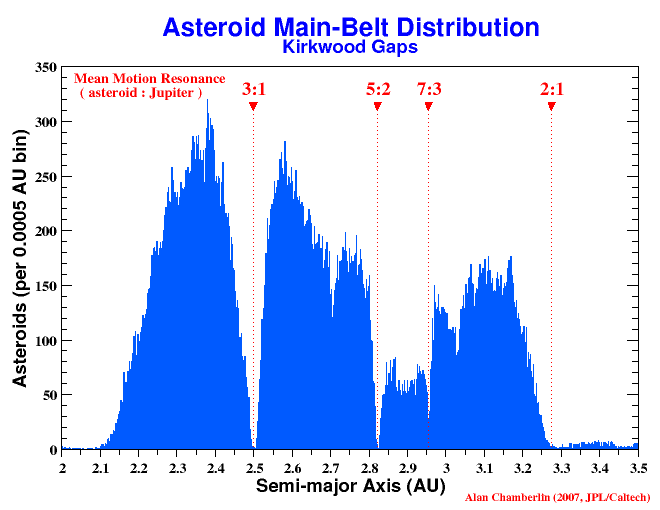
\includegraphics[width=\textwidth]{ast_histo-inverted.png}
\caption{Histogram plot depicting distribution of semi-major axis of 156,929 main-belt asteroids, created in June 2007 \cite{jpl_asteroid_web}.}
\label{fig:mbo_distribution}
\end{figure}
%

Asteroids don't only exist as single bodies in the Solar System, but they are also found in local multi-body systems consisting of two to even three asteroids. With advanced asteroid detection methods, astrophysicists have found over 190 multiple asteroid systems in the Solar System \cite{multipleAsteroids}. Contrary to intuition, these multiple asteroid systems exhibit a wide diversity in terms of the size ratios of the components, their mutual orbits and separation, implicating that the individual components evolved differently over time \cite{multipleAsteroids}. If a multi-asteroid system consists of two or three components, which are bound gravitationally, then it is termed as \textit{binary asteroids} or \textit{triple asteroids} respectively. Triple asteroids are also sometimes termed as \textit{trinary} or \textit{ternary} \cite{multipleAsteroidsTerminology}. Asteroid components that are not gravitationally bound but are genetically related, are termed as \textit{asteroid pairs}. Asteroid pairs where the larger asteroid is a binary or a triple asteroid, are termed as \textit{paired binaries} or \textit{paired triples}, respectively. The larger component in a binary or triple asteroid system or an asteroid pair, is referred to as the \textit{primary} and similarly the smaller component is referred to as the \textit{secondary} \cite{multipleAsteroidsTerminology}. Asteroids are further classified based on their dimensions and thermal properties, for which the reader should read the publication in \cite{multipleAsteroids}.

We now know what asteroids are and the different ways in which they are found in our Solar System, but is it important to study them? There are three major, and most commonly expressed, reasons to study asteroids in our solar system, and not just from a distance such as through radar telescopes placed on Earth, but also through in-situ exploration involving spacecrafts and surface probes. These reasons are mentioned as follows.
\begin{itemize}
\item Asteroids are basically the material left-over from formation of planets in our Solar System. Thus, they are the perfect source to study and understand the origins of the Solar System, as they have remained in the same pristine form since the birth of the Solar System, unlike the planets which have undergone massive topographical and atmospheric changes after their formation. The asteroids can provide valuable information on the chemical composition and initial conditions which led to the formation of planets, including Earth some 4.6 billion years ago. Several scientists have also hypothesized that water and life could have been brought about on Earth through an asteroid or comet and hence exploration of these small bodies could provide a definite answer to an age old question of how life began on Earth \cite{whyAsteroidsWeb}.
\item Asteroids have been hypothesized to have brought complex molecules to the surface of Earth that eventually resulted in life, but lately they have also been linked to the extinction of dinosaurs due to its impact with Earth. Earth is continuously bombarded with very small interplanetary material, most of which doesn't reach the surface of the Earth but gets evaporated in its atmosphere. However, every few 100 years, an asteroid spanning some tens of meter could impact Earth resulting in widespread damage, in the present case to life and property. But the impact from those will not cause the human race to extinct. But every 100,000 years or so, larger asteroids, spanning over tens of kilometer would impact the Earth, which will lead to extinction of life as we know it now. Although the probability of getting hit by an asteroid on such a large scale is low, it is still a statistical possibility and to be able to device strategies for active deflection of such asteroids, it is imperative that we understand more of the dynamics, properties and composition of the asteroids \cite{whyAsteroidsWeb}.
\item The third most important reason for us to study asteroids, is the fact that these small bodies are rich in raw materials or minerals. \gls{NEA} can be exploited for the resources that they possess and use it to build space structures or generate fuel for spacecrafts to enable human space exploration in farther reaches of the Solar System. By studying the asteroids, we can develop methods to tap the vast reservoirs of raw materials residing in them \cite{whyAsteroidsWeb}.
\end{itemize}

\section{Research problem}
In the previous section, we discussed what asteroids are and why its important to study them. In this section, we shall discuss, albeit broadly, the areas of research for the upcoming thesis work. The motivation for this literature study and the future thesis work arises from the fact that past in-situ space exploration activities have made use of explosive capsules to extract subsurface samples for analysis \cite{hayabusa2}. For asteroids with surface made of unconsolidated rock material or dust, use of explosive payloads to expose subsurface material could potentially result in the regolith being lofted from the surface of the asteroid. The lofted material could enter into a long term orbit, or a short term orbit concluding in re-impact of the lofted regolith back on the surface of the asteroid, or even escape the gravitational influence of the asteroid. This idea is fueled by a research paper \cite{idaEjectaErosion} which discusses the re-accretion and and escape of ejecta due to impact from impacts in the Ida system in the main-belt. The lofted regolith poses a serious threat to the safety of the spacecraft in orbit around the asteroid. To avoid any damage to it, it is necessary to develop models that can simulate the motion of the lofted regolith for a given asteroid, to as high an accuracy as possible, so that the mission design for asteroid exploration can account for it and ensure safety of the spacecraft. To do so we need to model the dynamics of the asteroid around the Sun, model the dynamical environment around the asteroid itself, and, although not limited to but also model the dynamics for multiple debris particles lofted from the asteroids surface and account for different perturbing forces that could affect the orbital motion of these particles. By running these simulation models we can compute trajectories for multiple particles at the same time and observe their long or short term behavior.

The tentative research questions shall be presented shortly. We say tentative because in the beginning, the report was aimed to focus on \textit{orbital motion of spacecraft around a binary asteroid system}. However, towards the period around which the report was being concluded, a thesis opportunity was offered from the \gls{CCAR} because of which the thesis topic was changed to \textit{orbital motion of regolith lofted from the surface of an asteroid}. The content of the report is nevertheless useful since it still discusses the dynamics around an asteroid with the difference that instead of a spacecraft, now it will be applied to lofted regolith material. Due to the sudden shift in the focus of the thesis at the time of writing this report, the research questions presented below should be considered as only tentative. The final research questions or problem statements will be mentioned in the final thesis report. The core questions are listed as follows:
\begin{itemize}
\item Simulate, observe and characterize the motion of regolith lofted from the surface of an asteroid for extended periods of time.
\item Does the lofted regolith enter a stable or unstable orbit? What are the corresponding initial conditions and can they be generalized for different asteroids?
\item What is the correlation, if any, between the size of the lofted material against stable or unstable orbital motion? Can a critical size for the lofted material be determined, for the asteroid under study, which would differentiate between stable and unstable orbital motion for the lofted material?
\item In case of stable orbits, are the orbits planar or spatial periodic?
\item In case of an unstable orbit, does the lofted regolith fall back to the surface of the asteroid or does it escape the gravitational influence of the asteroid? Can this behavior be also generalized for a different asteroid?
\item What is the subsequent motion of the regolith that re-impacts on the surface of the asteroid?
\item For a regolith sample return mission based on a touch-and-go technique (such as the \gls{OSIRIS-REx} mission), is it possible to retrieve a sample without causing adjacent surface material to be lofted in to an orbit around the asteroid?
\item For a subsurface sample return mission involving surface detonation (such as the Hayabusa-2 mission), how can the dangers of spacecraft damage from lofted regolith be averted or avoided?
\end{itemize}

\section{Outline of the report}
This literature study report tackles the problem of modeling particle dynamics and solving it in a systematic way. We begin by first describing the various missions that have been to asteroids in the past or are being operated currently along with missions planned for the future in \Cref{heritage}. \Cref{gravpot} discusses the various gravitational potential models that exist and have been applied in past for theoretical studies on orbital mechanics of or around asteroids along with the advantages and disadvantages of each model. \Cref{perturb} presents the relevant orbit perturbation models for working with particle dynamics around asteroids. \Cref{F2BP} begins with a brief introduction to relatively low-fidelity full two-body problem models that have been extensively applied in the past following which an extensive discussion on mutual potential and coupled equations of motion for binary polyhedron-based asteroids is presented. \Cref{RF3BP} begins by introducing the relatively low-fidelity restricted three-body problem but the chapter focuses more on the dynamics of a particle around binary asteroid modeled as two polyhedrons. A linearization technique to reduce simulation loads has also been introduced in that chapter. \Cref{integ} describes and compares the various numerical integration methods; an integrator is needed to propagate the orbital motion of a particle around an asteroid. \Cref{MCS} briefly describes the Monte Carlo simulation technique which will be utilized in our simulation package to generate multiple debris particles at the surface of an asteroid. \Cref{DST} presents some basic concepts on dynamical systems theory such as poincar\'e maps which are used when one wants to characterize the motion of an orbiting particle. And finally, \Cref{conclusion} concludes the literature study report.

\part{Motivation}
\chapter{Heritage}
\label{chap:heritage}
\graphicspath{{Mission_Heritage/Images/}}

In the past, there have been multiple spacecraft missions to the small bodies in our Solar System which have collectively increased our understanding about them. While a large majority of these have been asteroid fly-by scenarios, a few have also been rendezvous missions \parencite{esa_mission2asteroids_web}. This chapter will provide an overview on few of these missions followed by a brief literature review which shall be of interest to the thesis at hand. This will help us in justifying the research objectives mentioned in \Cref{chap:research_questions}. \Cref{sec:past_missions} will discuss the asteroid rendezvous missions which have already taken place, \Cref{sec:future_missions} will discuss future rendezvous missions, and finally, \Cref{sec:literature_review} will discuss the state-of-the-art.

\section{Past Missions}
\label{sec:past_missions}
In all the history of space exploration there have been only three spacecraft missions that have rendezvoused with asteroids. In chronological order these are: \gls{NASA}'s \gls{NEAR}-Shoemaker mission to asteroid Eros, \gls{JAXA}'s Hayabusa mission to asteroid Itokawa, and \gls{NASA}'s Dawn mission to asteroids Vesta and Ceres \parencite{scheeresBook}. Out of these, only \gls{NEAR} and Hayabusa had direct contact with the small bodies and acquired high-resolution imagery of surface regolith.

\subsection{NEAR-Shoemaker}
\label{subsec:near_heritage}
The \gls{NEAR}-Shoemaker (henceforth \gls{NEAR}) mission was launched in 1996 and rendezvoused with Eros in 2000. Its operational phase around the asteroid continued for about a year during which it obtained several high-resolution images of the surface and collected comprehensive measurements to estimate its internal mass distribution, shape model, gravity and spin state amongst other observations \parencite{scheeresBook}. The bulk density of Eros was estimated to be $2.67 \pm 0.03 [g/cm^3]$ and its mass to be $(6.6904 \pm 0.003) \times 10^{15} [kg]$. The rotation state was estimated to be $1639.38922 \pm 0.00015$ [deg/day] which gives a rotational period of about $5.27$ [hrs] \parencite{erosShapeDetermination}. On 25 October 2000, \gls{NEAR} executed a \gls{LAF} over Eros in which it acquired several high-resolution images that helped in understanding the surface morphology. The images confirmed the existence of a substantial amount of regolith on the surface with a typical thickness value of tens of metres over the bedrock, except of course on steep slopes. The regolith was found to be highly complex, in that it varied from fine material to metre-sized ejecta blocks \parencite{Veverka2001}. \cite{Robinson2001} estimates the size of the finer regolith to be around 1.0 [cm] or smaller from images that had a resolution of 1.2 [cm] per pixel. \Cref{fig:eros_regolith} depicts the regolith morphology in one of the high-resolution imaging sequences from the \gls{LAF} \parencite{veverka2001landing}.
%%%
\begin{figure}[htb]
\centering
\captionsetup{justification=centering}
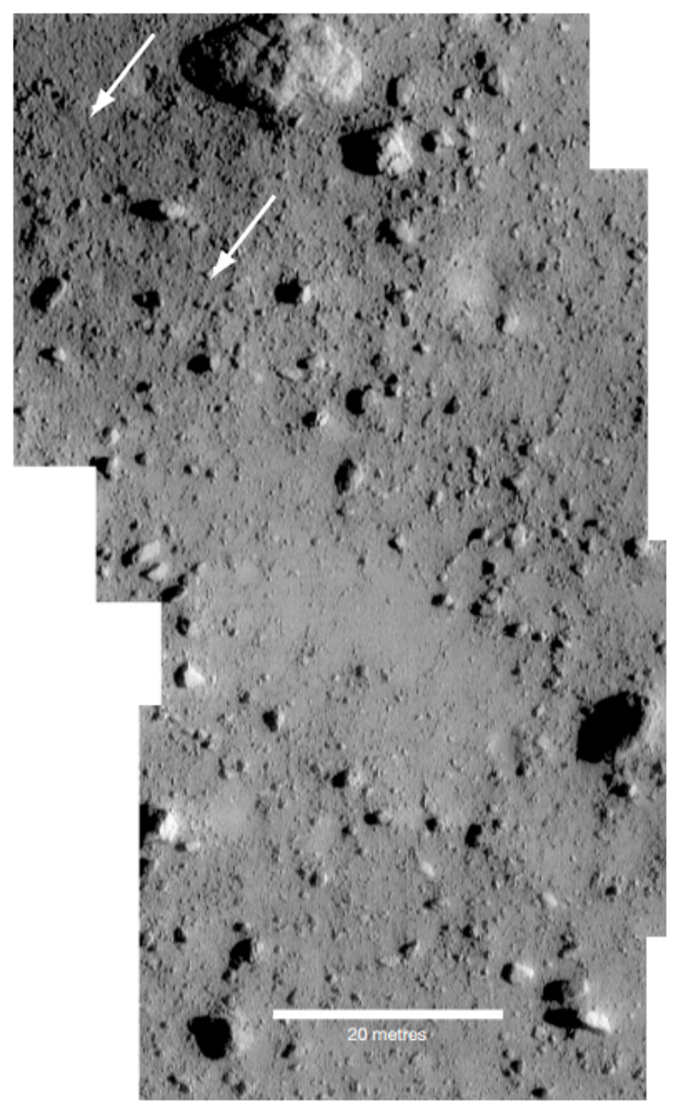
\includegraphics[width=\linewidth, height=0.5\textheight, keepaspectratio=true]{eros_regolith.pdf}
\caption{Mosaic of high-resolution images depicting the nature of regolith on the surface of Eros \parencite{veverka2001landing}.}
\label{fig:eros_regolith}
\end{figure}
\FloatBarrier
%%%

\subsection{Hayabusa}
\label{subsec:hayabusa_heritage}
The Hayabusa spacecraft was launched by \gls{JAXA} in 2003 and it arrived at asteroid Itokawa in 2005. After arrival, it performed close-proximity operations around the asteroid for approximately 3 months during which several measurements were taken to estimate the shape, mass, topography and elemental composition of the asteroid. During this period, the spacecraft also collected samples from the surface of the asteroid that were eventually returned back to Earth in 2010. The measurements at Itokawa estimated its mass to be $3.51 \times 10^{10}$ [kg] and its bulk density to be $1.9 \pm 0.13$ [g/$cm^3$] \parencite{fujiwara2006ItokawaHayabusa}.
%
\newline\newline
%
Two distinct types of terrains can be recognized on Itokawa, one which is rough and rich in boulders and the other which is smooth and mostly flat. This distinction can easily be seen in \Cref{fig:itokawa_regolith}. The smooth regolith regions, that account for approximately 20\% of Itokawa's surface, composed of fragmented debris with grain sizes ranging from sub-centimetre to centimetre scales. One of the smooth regolith regions, called Muses Sea and from where the sample was also acquired, even consisted of a few metre-sized boulders that were hypothesized to have landed in the region as secondary ejecta \parencite{miyamotoItokawaRegolith}. The rougher terrain on Itokawa, which has a very sharp boundary with the smoother regolith filled regions (as evident in \Cref{fig:itokawa_regolith}), consists of boulders that range upto tens of metres in size \parencite{fujiwara2006ItokawaHayabusa}.
%%%
\begin{figure}[htb]
\centering
\captionsetup{justification=centering}
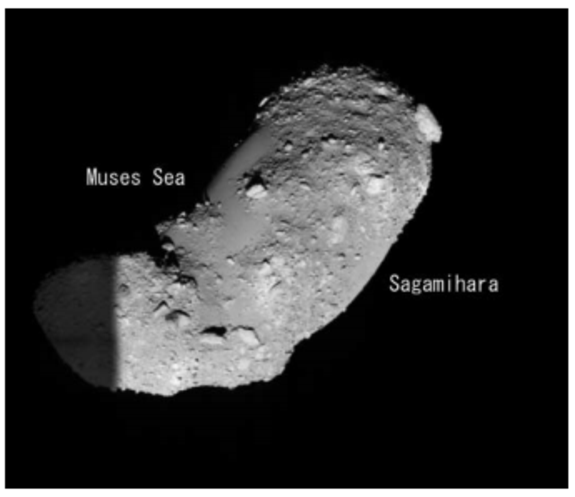
\includegraphics[width=\linewidth, height=0.4\textheight, keepaspectratio=true]{itokawa_regolith.pdf}
\caption{Image of Itokawa taken from a 7 [km] altitude depicting the nature of regolith on its surface. Muses Sea and Sagamihara are the two distinct smooth regolith regions on the asteroid \parencite{fujiwara2006ItokawaHayabusa}.}
\label{fig:itokawa_regolith}
\end{figure}
\FloatBarrier
%%%
Hayabusa employed an \textit{impact sampling mechanism} that would work across various types of terrains, from hard bedrock to fine regolith. The spacecraft consisted of a long cylindrical sampling horn with a conical tip. When the tip of the horn touched the surface of the asteroid, the deformation in the horn's fabric was detected by a laser range finder and within 0.3 [s] of this event, a 5.0 [g] projectile was fired towards the surface with a velocity of 300 [m/s] and the resultant ejecta was collected by the sampler \parencite{yano2004sampling}. \cite{yanoHayabusaTouchdown} presents data from the sampling experiments that were performed on ground in $1g$ and micro-gravity environments. The experiments revealed that, for the projectile hitting at normal impact angles in micro-gravity, the impact ejecta mass of particles greater than 1.0 [cm] ranged from 2 - 11 [g] whereas for particles less than 1.0 [mm] the ejecta mass ranged from 100 - 10000 [g]. The impact target consisted of various analog materials from glass beads to lunar regolith simulant and an experiment like is a nice indicator of how artificial impact events can displace significant amount of fragmented debris on an asteroid.

\section{Future Missions}
\label{sec:future_missions}
We will now discuss two missions, Hayabusa-2 by \gls{JAXA} and \gls{OSIRIS-REx} by \gls{NASA}. Both are currently en route to their respective target asteroids and after orbit insertion, they shall perform operations to collect surface samples.

\subsection{Hayabusa-2}
\label{subsec:hayabusa2_heritage}
Hayabusa-2 is the second asteroid sample return mission by \gls{JAXA}, which to a significant extent, shares the successful technical legacy of Hayabusa. The target asteroid of the former is \textit{1999 JU3} which is suspected to contain organic matter and hydrated minerals \parencite{TsudaHayabusa2SystemDesign}. The shape model of the asteroid, also designated as \textit{Ryugu}, is shown in \Cref{fig:ryugu_shape} \parencite{ryuguShapeModel}. A successful sample return from this asteroid may thus help us in understanding the origin of life and/or water on Earth. The spacecraft will enter into an orbit around its target by mid-2018, after which it will perform close-proximity operations for 1.5 years. The mission will entail 3 touchdowns for sample acquisition and a cratering event to observe the subsurface of the asteroid. The sampling mechanism is based on that of Hayabusa and each sampling attempt has the potential to acquire samples in the order of 100 [mg]. The samples are sealed-off and transported back to Earth in a re-entry capsule. The cratering operation is performed by a \gls{SCI}. The \gls{SCI} is deployed by the spacecraft at an altitude of 500 [m] and after a preset time, a detonation accelerates it to about 2 [km/s] prior to impact. It is estimated that this will result in a crater of about 2 [m] wide. Prior to the detonation of \gls{SCI}, the spacecraft will move to a safe location on the opposite side of the asteroid from the impact point to avoid damage from impact ejecta and/or debris from the detonation. Apart from these, the spacecraft will perform other in-situ operations to characterize the asteroid and will also deploy a lander and three miniature rovers for technology demonstration \parencite{TsudaHayabusa2SystemDesign}.
%%%
\begin{figure}[htb]
\centering
\captionsetup{justification=centering}
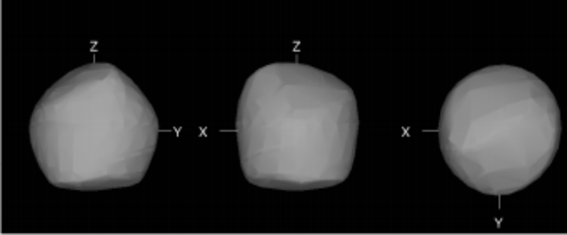
\includegraphics[width=\linewidth, height=0.3\textheight, keepaspectratio=true]{ryugu_shape.pdf}
\caption{Ryugu shape model as estimated from the observations made by Herschel Space Observatory, supported by several ground-based measurements and data from other space-based assets \parencite{ryuguShapeModel}.}
\label{fig:ryugu_shape}
\end{figure}
\FloatBarrier
%%%

\subsection{OSIRIS-REx}
\label{subsec:osiris_heritage}
\gls{OSIRIS-REx} is part of \gls{NASA}'s New Frontiers program and will travel to \gls{NEA} 1999 $RQ_{36}$, also known as Bennu. The shape model of the asteroid is shown in \Cref{fig:bennu_shape} \parencite{bennuShapeModel}. The mission, amongst other scientific objectives, will return a regolith sample back to Earth that may provide insight into the initial states of planetary formation as well as answer questions on the origins of life. Since Bennu is a \gls{NEA}, the sample collection and subsequent analysis will provide us information on asteroids that could potentially impact Earth. The spacecraft was launched in 2016 and is expected to reach its target by the end of 2018 \parencite{berry2013osiris}. The asteroid has a semi-major axis of 1.126 [AU] which makes it an easily accessible asteroid as far as distance is concerned. But more than that, Bennu falls under the category of asteroids that are rich in volatiles and could potentially be related to objects that brought the seeds of life to Earth. Initial observations of Bennu through ground based telescopes, the Spitzer Telescope, the Arecibo Observatory and other assets revealed an abundance of regolith on the surface with grain sizes ranging from 4 - 8 [mm]. \gls{OSIRIS-REx} will acquire the regolith sample using a \gls{TAG} mechanism which uses pressurized Nitrogen gas to force the loosely held regolith into a collection chamber. The sampling will occur in 2020 and it will be retrieved on Earth in 2023 \parencite{osirisMissionOverview}.
%%%
\begin{figure}[htb]
\centering
\captionsetup{justification=centering}
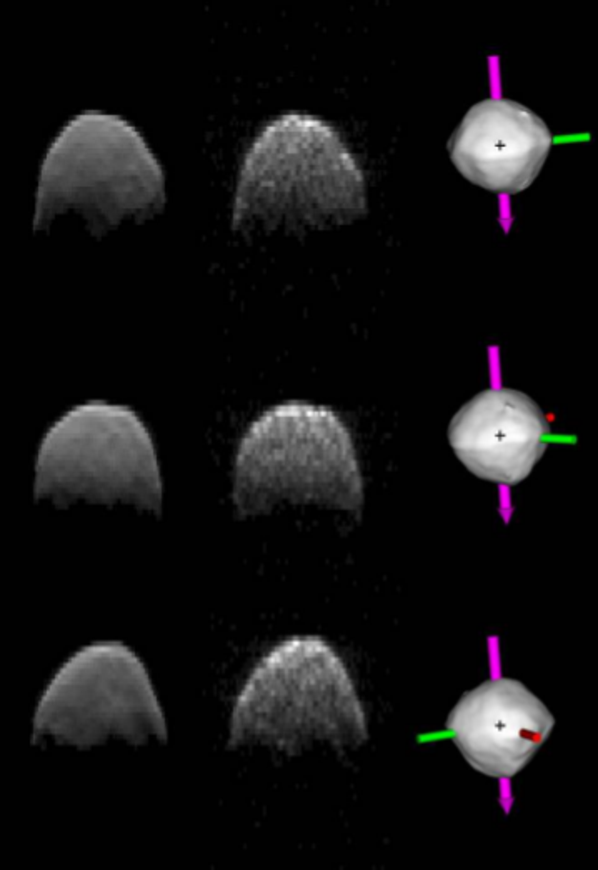
\includegraphics[width=\linewidth, height=0.4\textheight, keepaspectratio=true]{bennu_shape.pdf}
\caption{Bennu's shape as observed from the radar data collected by the Goldstone and Arecibo observatories (shown in middle column of the image). The left column displays the model that provides the best fit to the radar data and the right column shows the final estimated 3D model of Bennu as it would appear in the sky \parencite{bennuShapeModel}.}
\label{fig:bennu_shape}
\end{figure}
\FloatBarrier
%%%

\section{State of the art / Literature Review}
\label{sec:literature_review}
In this section we shall discuss a few research papers relevant to this thesis; the techniques they applied to understand the orbital behavior of impact ejecta and the shortcomings of these studies.
%
\newline\newline
%
A good starting point to understand the topic at hand is provided by \cite{scheeres2002fate}. It reviews the gravity and perturbing force models along with the dynamical equations of motion for a particle in orbit around an asteroid \& the model for generating initial conditions to launch ejecta from the surface of an asteroid. It also mentions about existing analytical methods to compute guaranteed escape and re-impact speeds for impact ejecta i.e. speeds at which particles would immediately escape or re-impact after being launched. \cite{scheeres2002fate} also discusses the various numerical and analytical methods that have been used in literature for analyzing the motion of particles that stay in a pseudo-stable orbits for extended periods of time before meeting their final fate. It also presents various mechanisms that have been hypothesized for the capture-case scenario i.e. particles that stay in orbit around asteroids for a relatively long time, from hundreds of days to several asteroid years. The analysis of these capture orbits, in particular, has been done by considering the Solar perturbations and irregular gravity effects of the asteroid but always in isolation.
%
\newline\newline
%
\cite{richter1995stability} provides an analytical method to solve for the motion of particles around a non-rotating, spherical cometary nuclei which is on an eccentric, heliocentric orbit. In their paper, they ignore Solar tidal effects and assume that the particle motion around a homogeneous spherical body would experience weak perturbations from \gls{SRP}. They give averaged equations for the variation of eccentricity and angular momentum vectors as a function of the true anomaly of comet around the Sun. The paper also discusses the limitations and validity of using their analytical approximation as well as the conditions for collision-free orbits for small and large dust particles around the comet. Although the study conducted by \cite{richter1995stability} is for comets, it can be extended to asteroids as well and has been used by \cite{morrow2001solar} for analyzing solar sail powered trajectories around them. \cite{lee1996dust} discusses the electrostatic levitation of dust particles from the surface of an asteroid. It uses two electrostatic field production methods used in the study of dust levitation on moon, and applies them to the case of an asteroid. The study does not involve the orbital motion of dust particles but it does provide conditions which could cause the dust particle to escape in the event of electrostatic levitation.
%
\newline\newline
%
\cite{scheeres1996orbits} provides an extremely detailed and systematic study of particle dynamics close to the surface of asteroid Castalia. They include the effect of the irregular shape of the asteroid on orbital dynamics by using a spherical harmonics model of degree and order upto 4 in simulating the gravity potential. They also derive analytical results for computation of guaranteed return and escape speeds as a function of location of particle on the surface of the asteroid. The paper employs dynamical systems theory and investigates the use of stable manifolds associated with orbits around equilibrium points and intersecting the surface of the asteroid, to obtain the initial launch conditions for the particle that will lead to a temporary stable orbit around the asteroid. \cite{scheeres2000ejecta} applies the radiation pressure approximation method developed by \cite{richter1995stability} to study the temporary capture of particles in an orbit around a comet but improves it to account for the comet's rotation as well. The results obtained from the analytical approximation are compared with the results from the numerical simulation wherein the latter accounts for other perturbations as well such as Solar Tidal effect and gravity field variations. The comparison showed that the radiation pressure approximation method by \cite{richter1995stability} is qualitatively correct and can be used for statistical studies at the very least. They were also able to establish qualitative ranges on ejecta velocity and angles that result in capture orbits, an example of which is shown in \Cref{fig:comet_temporary_capture_example}.
%%%
\begin{figure}[htb]
\centering
\captionsetup{justification=centering}
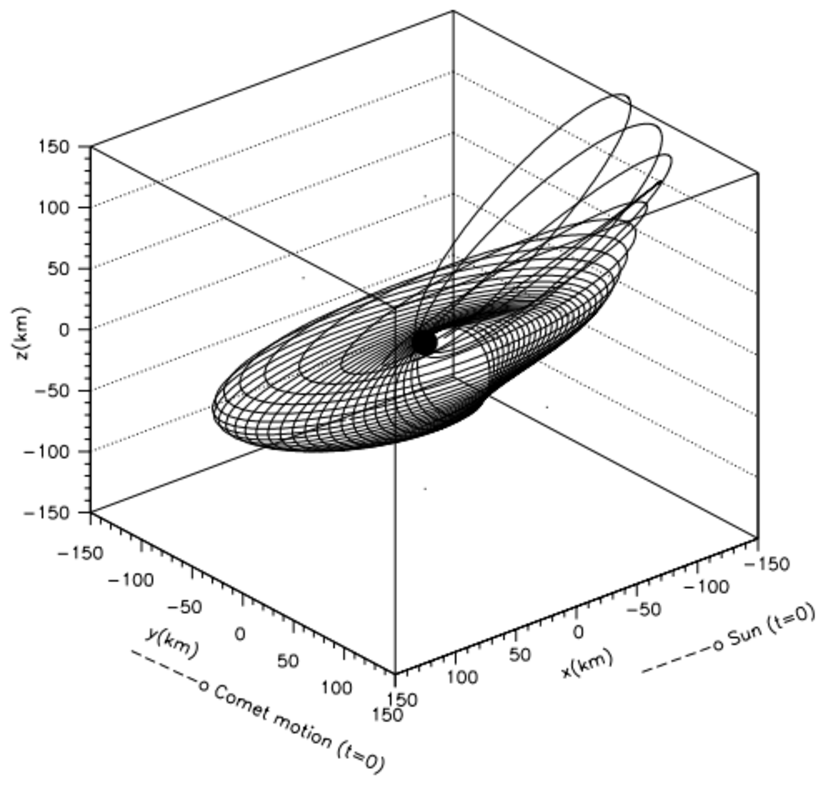
\includegraphics[width=\linewidth, height=0.4\textheight, keepaspectratio=true]{capture_orbit_tempel1_scheeres.pdf}
\caption{Example of single particle capture trajectory around comet Tempel-1 \parencite{scheeres2000ejecta}.}
\label{fig:comet_temporary_capture_example}
\end{figure}
\FloatBarrier
%%%

\cite{korycansky2004_impactEjecta} conducts a study to understand the distribution of impact ejecta and its connection with existing regolith on the surface of asteroid 433 Eros. The study involves the use of Monte Carlo simulation technique to observe the orbital evolution of a large number of test particles from randomly selected locations on the asteroid. They use a coarse polyhedron model of asteroid Eros to model its gravitational field, thus accounting for gravity perturbations. However, the research does not account for perturbations from \gls{SRP}. \cite{yarnoz2014passive} studies the orbital motion of lofted regolith in the context of using Solar Radiation Pressure to passively sort asteroid material. They use semi-analytic methods to derive conditions that would cause regolith to either escape or re-impact the asteroid’s surface. They make use of the radiation pressure approximation methodology developed by \cite{richter1995stability} in their semi-analytical approach. However, the affect of an irregular shape of an asteroid, i.e. gravity perturbations, is not accounted for in their calculations.
%
\newline\newline
%
In general, we witnessed minor drawbacks in these studies such as not always accounting for gravity and Solar perturbations together, or the derivation of an analytical solution which is not globally valid. Some studies involved both analytical and numerical methods for simulating orbital dynamics but even then the numerical approach was more for comparing the validity of the analytical solution and not as much for obtaining the full range of initial conditions that will lead to re-impact, escape or temporary capture of regolith around an asteroid. The affect of launch direction of regolith was also not considered in most of the studies, especially the ones that applied analytical methods. We have attempted to address these shortfalls to better understand the reasons for the complex orbital behavior of particles launched from the surface of an asteroid, by following a numerical simulations approach instead of an analytical approximation or a dynamical theory one (see \cite{scheeres2002fate} for a brief discussion between the three methods for analyzing orbital behavior of asteroid ejecta). We have accounted for gravity and Solar perturbations while simulating trajectories for particles of different sizes and density. These perturbations have been considered in isolation as well as together to witness the effect of each individual perturbation on a particle trajectory. More details on the dynamics involved, the numerical simulator, and the methodology will be presented later in this report.


\chapter{Research Questions \& Goals}
\label{chap:research_questions}
\graphicspath{{Research_Questions/Images/}}

The study of the dynamics of a particle, on or around an asteroid, can be broadly divided into three main regimes. The first regime involves the study of surface ejecta generation, from natural events such as interplanetary particle impacts, cratering by other asteroids \& electrostatic dust levitation, or from space exploration events where the natural state of the regolith is disturbed by spacecraft sampling activities. The second regime involves the study of the subsequent orbital behavior of impact ejecta or lofted regolith under varying parameters such as launch conditions, asteroid rotational state \& shape, regolith particle size and density, Solar phase etc. And finally, the third regime involves the study of particle dynamics when it re-impacts with the surface of the asteroid. This thesis will concern itself with the second regime of research, i.e., the natural orbital evolution of regolith lofted from an asteroid’s surface.
%
\newline\newline
%
As mentioned earlier in \Cref{chap:intro}, understanding particulate environment around small-bodies has been identified by \gls{NASA} as a strategic knowledge gap. Understanding and developing tools or knowledge to estimate the orbital behavior and final fate of lofted regolith with greater accuracy is important for future space exploration missions (see \Cref{sec:future_missions}) that will involve direct interactions with asteroids, to avoid any damage to the spacecraft or surface robotic crew from orbiting particles. High-fidelity simulations of particulate motion can also help scientists in understanding the surface morphology of asteroids by helping them recreate cratering events. In \Cref{sec:literature_review}, we highlighted the shortfalls in the research done on the topic so far and we identified a gap that needs to be filled, and hence, the following top level research question is set:
\vspace{5mm}
%%%
\begin{center}
    \fbox{\parbox{0.8\textwidth}{
    \centering
    \textbf{\textit{Can we explain the orbital behavior and eventual fate of lofted regolith around an asteroid in presence of gravity and Solar perturbations?}}}
    }
\end{center}
%%%
\vspace{5mm}
This top-level research question is divided into the following sub-questions that help in structuring the thesis:
%%%
\begin{enumerate}
\item Does the regolith, launched from different locations such as leading, trailing, longest and shortest edge of an asteroid, show characteristic differences with regard to its final fate?
\item Can clear demarcation be established between the re-impact, capture, and escape scenarios, for the lofted regolith, based solely on the initial conditions?
\item What causes the regolith to enter into a temporary capture orbit around the asteroid?
\item For the same launch conditions, how does the orbital behavior and final fate of the regolith differ for different particle sizes and densities?
\item For the same particle size and density, how does the orbital behavior and final fate change with different launch locations?
\item Can we establish a non-conservative analytical expression to determine guarantee escape speed in presence of perturbations?
\item Can we exploit the orbital behavior of lofted regolith for sorting material of different sizes and densities as an application for asteroid mining?
\end{enumerate}
%%%
\vspace{5mm}
In order to answer these questions, the following main research goal is set:
%%%
\begin{center}
    \fbox{\parbox{0.8\textwidth}{
    \centering
    \textbf{\textit{Investigate the orbital motion of regolith launched from the surface of an asteroid using numerical simulations.}}}
    }
\end{center}
%%%
The sub-research goals are mentioned as follows:
%%%
\begin{enumerate}
\item Develop a modular and robust software tool that can propagate the trajectory of spherical particles around an asteroid for given initial conditions.
\item Develop software tools to plot and analyze numerical simulation results
\item Validate the software tools.
\item Perform simulations for particles launched from the asteroid's surface with different initial conditions, launch locations, and for different particle sizes \& densities.
\item Perform qualitative and quantitative analysis on numerical simulation results.
\item Document results and inferences for thesis report and peer reviewed journal paper.
\end{enumerate}
%%%
The vast majority of the time will be spent on designing the simulator and data processing \& visualization tools (see \Cref{chap:naos}), followed by their verification and validation (see \Cref{chap:v_and_v}). A relatively smaller time would then remain to perform the research and investigate the results, however the time remaining for this would be sufficient to answer all our research questions.

\part{Dynamics Modeling}
\chapter{Orbital dynamics around Asteroids}
\label{chap:dynamics_modeling}
\graphicspath{{Modeling/Images/}}

This chapter will focus on accurate modeling of the asteroid environment and the equations of motion of a particle around it in presence of gravity and Solar perturbations.

\section{Modeling Assumptions}
\label{sec:assumptions}
The simulator \footnote{The simulator is called \gls{NAOS} and can be downloaded from \url{https://github.com/agrawalabhishek/NAOS/tree/devcode2}} designed as part of this research involves some degree of approximation of the real-world dynamical environment around the asteroid. Every degree of freedom and complexity added to a simulator to resemble the real-world, will also act as a potential source of error. By designing a relatively simple simulator, we can explain the characteristic behavior of regolith through fundamentals while keeping the sources of error as low as possible. Of course, we verify the simulator (see \Cref{chap:v_and_v} for a detailed verification and validation process) but by including a higher degree of fidelity in the simulator, we increase the workload on the verification process as well, thereby reducing the scientific output in the end. Moreover, the current simulator and the results from it will act as a benchmark for a higher-fidelity simulator in the future. Thus, the approximations made in this thesis are as follows:
% Every research involves some degree of approximation of the natural world, on Earth or otherwise, to understand or explain any phenomenon. Through this thesis work, we hope to understand the orbital behavior of regolith around an asteroid and we have to do it with a relatively simplified model because recreating an exact replica of an asteroid's dynamical environment is out of the scope of this thesis. Although we are making simplifications, but it does not mean that the scientific returns from it would be any less. The particle trajectories might not be exact when we conduct the simulation based experiments in real world but the underlying science explaining the orbital behavior would remain unchanged (this would become more clear in \Cref{chap:results}). Thus, the simplifying assumptions we make for modeling the asteroid-regolith system are mentioned as follows:
%%%
\begin{enumerate}
\item The asteroid body is modeled as a smooth triaxial ellipsoid to account for its non-uniform gravity. The triaxial model is chosen over the spherical and ellipsoidal harmonics approach because we want to study the motion of regolith close to the surface of the asteroid; in particular the re-impact scenarios. This can not be done with the harmonics model as the gravity potential diverges, within the circumscribing volume, from the true potential of an irregular body. We chose to not use a polyhedron model either, even though it can account for surface irregularities of an irregular body much better than the triaxial ellipsoid. This decision was made to reduce the complexity of the simulator, however, we do not sacrifice on the qualitative aspect of the results since the triaxial model also provides a non-uniform gravity field.
% This is because we want to decouple the fundamental phenomenon, associated with the motion of the regolith, from any effects of a truly irregular shape such as in the case of a polyhedron model.

\item Craters, surface depressions, mountains and any other terrain deformity on the asteroid are not considered in the simulation. The body is considered to have a uniform density. This is to simplify calculations of the gravitational acceleration.

\item The asteroid is rotating uniformly about its shortest axis. This is considered for simplicity and also because most Solar System bodies would dissipate energy to eventually enter a rotational state that is uniform and about its axis of maximum moment of inertia \parencite{scheeresBook}. Hence, the approximation for the asteroid remains valid.

\item The regolith grains are assumed to be spherical in shape to simplify the \gls{SRP} calculation as the cross-sectional area of a sphere would remain the same irrespective of its attitude. In addition to this, the grains are assumed to have an albedo equal to one, which means that any impinging Solar photons are completely reflected and this is done to account for maximum perturbation from \gls{SRP} for a given location and area-to-mass ratio (see \Cref{subsec:srp} for more details).

\item Multiple regolith particles are launched from a given location on the asteroid in the form of a cone to replicate ejecta from a cratering event. But all particles are assumed to be coming off from the same point, unlike that in the case of an actual cratering event. This is because the pretext of the thesis was that the regolith is lofted due to an activity from a spacecraft which would result in relatively smaller craters or surface depressions. Thus assuming that all particles in this \textit{"ejecta cone"} emerge from the same point on the asteroid is reasonable and simplifies the simulation.

\item The slant angle of the \textit{"ejecta cone"} (henceforth the declination angle) from the local surface normal is kept constant at \SI{45.0}{\degree} (which is a middle value in the entire declination range from \SI{0.0}{\degree} - \SI{90.0}{\degree}). We want to consider a general case and not introduce another degree-of-freedom in terms of varying declination angles, however, it should be noted that the results from simulation for any other declination angle would be different. There is an exception to the fixed declination angle assumption though; only in \Cref{chap:nonconservative}, we use a range of declination angles at which regolith is launched.

\item The calculations were subjected to simulate a maximum of 270 days and were terminated earlier if a particular trajectory resulted in escape or surface re-impact. This number was obtained by looking at the close-proximity operational time periods of exploration missions to small bodies of our Solar System. We wanted a maximum simulation time in the context of a man-made mission and hence this approach was taken. We accounted for four missions, two from the past and two planned for the future, which have direct contact with a small body as part of their mission and continued the mission around the small body afterwards (hence, not just disposal and/or fly-by). These are the Philae (Rosetta), Hayabusa, Hayabusa-2, and the \gls{OSIRIS-REx} missions. The close-proximity design operation time period for the Philae lander was three months \parencite{philaeMissionTimeline}, three months for Hayabusa \parencite{hayabusaCloseProximity}, eighteen months for the Hayabusa-2 mission \parencite{TsudaHayabusa2SystemDesign}, and finally twelve months for the \gls{OSIRIS-REx} mission \parencite{osirisMissionOverview}. The average of all of this comes out to be nine months, which is what we have considered to be the maximum simulation time. In this regard, we are also categorizing orbital behavior that does not result in escape or re-impact in those 270 days, as capture orbits.

\item The loss of material and mass from the asteroid, when the regolith is lofted from the surface, is not modeled in the simulation since it is assumed that a very small amount of material will be displaced by a spacecraft activity (impact and/or sampling). This assumption is based on the sample collected by the Hayabusa mission (see \Cref{sec:past_missions} and the references therein).

\item Interaction between individual regolith grains is not accounted for because we are simulating multiple particles being lofted at the same time and granular interaction on such a scale would be extremely complex and small and beyond the scope of this thesis.

\item Secondary motion of regolith, after re-impacting the surface, is not modeled and it is assumed that the particles just come to a standstill.

\item The shadow region of the asteroid is not modeled which means that the solar perturbations are always acting on the regolith grain. This simplification was made since asteroids are extremely small compared to planets, and thus, the chances of an orbiting particle spending long periods of time in the shadow are very small.

\item Perturbations are considered only from the Sun. \gls{SRP} is important because regolith grains will have higher area-to-mass ratios, relative to a spacecraft, and so the radiation pressure would be significantly large for them. We model the third-body attraction from the Sun (\gls{STBE}) as well but not from any of the planets because we are assuming that the small body does not pass close to any planet, thus rendering the perturbations from them insignificant.
% The magnitude of perturbation from the \gls{STBE} itself is atleast 5 orders of magnitude smaller than the gravitational acceleration (for a sample asteroid assumed to be in a circular orbit at 1 AU from the Sun) when the regolith is in close proximity to the asteroid (see \Cref{chap:results}).

\item The apparent motion of the Sun around the asteroid is considered circular and in the equatorial plane of the asteroid, again, to restrict another degree of freedom in the simulations and consider a general case.
% \item The apparent motion of the Sun around the asteroid is considered circular and in the equatorial plane of the asteroid; this was based on the orbital element measurements of all observed asteroids. The majority of these asteroids have small orbital eccentricities \parencite{malhotra2016_eccentricityDistribution}. \cite{jedicke1998_orbitalElements} presents debiased measurements for the inclination of the \gls{MBO} and shows that a large number of asteroids have near-zero inclinations.
\end{enumerate}
%%%
\newpage
\section{Reference Frames}
\label{sec:reference_frames}
Before describing the motion of regolith around the asteroid, it is important to define the frames of reference with respect to which this motion is defined and the transformation of state vectors between these frames. We use two asteroid-centric reference frames, both of which are depicted in \Cref{fig:reference_frame}. Since we will be using a triaxial ellipsoid to model an asteroid (for details, see \Cref{sec:gravity}), the body-fixed rotating frame and the inertial frame with respect to this model are shown in \Cref{fig:ellipsoid_rotating_frame,fig:solar_phase_and_inertial_frame} respectively.
%%%
\begin{figure}[htb]
\centering
\captionsetup{justification=centering}
\includegraphics[width=\textwidth, height=0.30\textheight, keepaspectratio=true]{reference_frames.pdf}
\caption{Two asteroid-centric reference frames, one being inertial (depicted by solid lines and the subscript I) and the other being a body-fixed rotating frame (denoted by dashed lines and the subscript B). The position vector to a regolith particle is shown as $\protect\vv{\bm{r}}_{P,B}$, whereas the position vector to the Sun is shown as $\protect\vv{\bm{r}}_{S,I}$.}
\label{fig:reference_frame}
\end{figure}
\FloatBarrier
%%%
The two frames are defined as follows:
%%%
\begin{enumerate}
\item \gls{AIF} - This is a non-rotating frame fixed inertially in space with its origin at the centre of mass of the asteroid. \Cref{fig:solar_phase_and_inertial_frame} shows the orientation of the frame (in x-y plane) such that the x-axis is pointing to the Sun when the longitude of the Sun (or effectively the true anomaly of the apparent circular motion of the Sun around the asteroid) $\vartheta$ is zero. The y-axis, thus, points to the Sun when $\vartheta = 90^o$ and finally the z-axis is obtained by following the right-hand rule, coming out of the sheet in 3D.
%
\item \gls{ARF} - This frame is fixed to the rotating asteroid with its origin at the centre of mass of the asteroid and its axes aligned with the principle axes of the asteroid. \Cref{fig:ellipsoid_rotating_frame} shows the orientation of this frame, assuming a triaxial ellipsoid model (for details see \Cref{sec:gravity}). The x-axis is pointing along the longest axis of the triaxial ellipsoid, and the z-axis is pointing along the shortest axis. It is also aligned with the $z_I$-axis of the \gls{AIF} as shown in \Cref{fig:reference_frame}. The y-axis points in the direction of the remaining third axis, satisfying the right-hand rule. The asteroid (and effectively the \gls{ARF}) is rotating in a counter-clockwise sense with respect to the \gls{AIF}, with constant angular velocity $\omega$ about the $z_B$-axis as depicted in \Cref{fig:reference_frame}.
\end{enumerate}
%%%
%%%
\begin{figure}[htb]
\centering
\captionsetup{justification=centering}
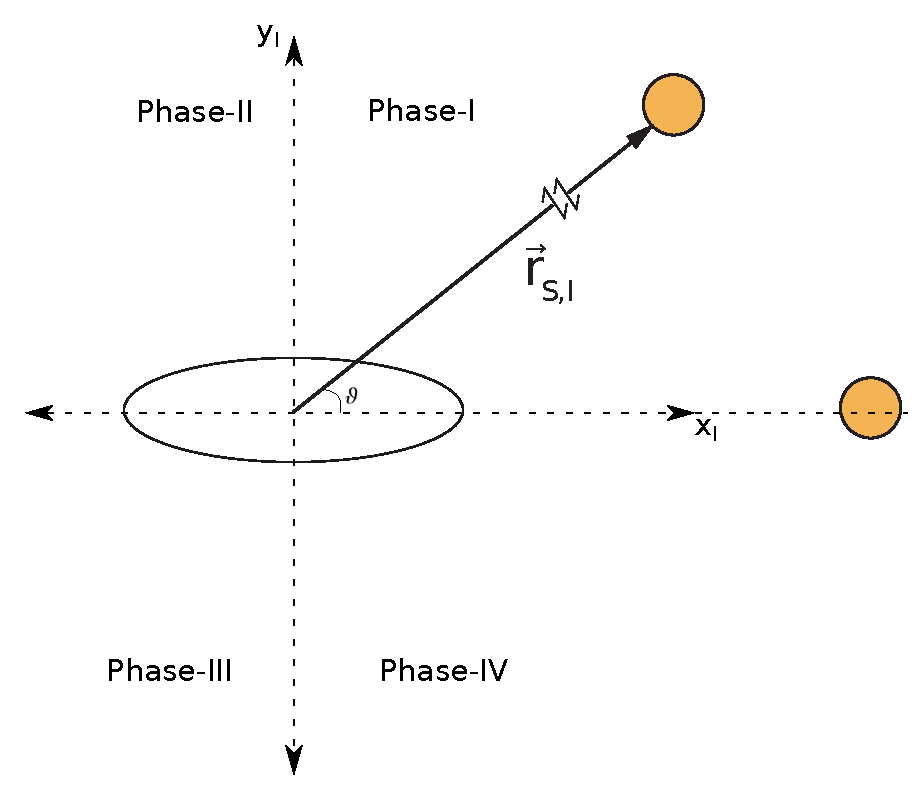
\includegraphics[width=\textwidth, height=0.35\textheight, keepaspectratio=true]{solar_phase_and_inertial_frame_3.pdf}
\caption{Asteroid-centric inertial frame x-y plane. The position vector to the Sun is shown as $\protect\vv{\bm{r}}_{S,I}$ with $\vartheta$ as the longitude of the Sun (or effectively the true anomaly). The four phases are for a broader identification of the Sun's location with respect to the asteroid.}
\label{fig:solar_phase_and_inertial_frame}
\end{figure}
\FloatBarrier
%%%
%%%
\begin{figure}[htb]
\centering
\captionsetup{justification=centering}
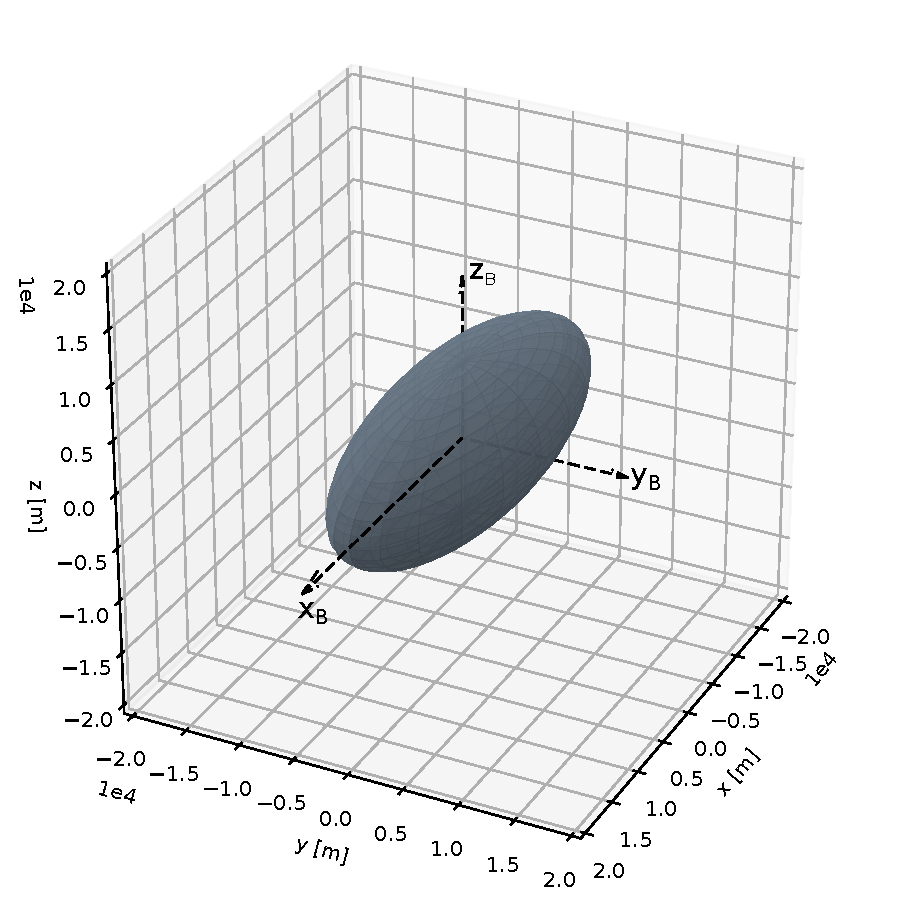
\includegraphics[width=\textwidth, height=0.35\textheight, keepaspectratio=true]{body_fixed_ellipsoid_frame.pdf}
\caption{Representation of the body-fixed rotating frame for a triaxial ellipsoid model of an asteroid. $\bm{x_{B}}$ is aligned with the longest axis, $\bm{z_{B}}$ is aligned with the shortest axis and $\bm{y_{B}}$ is aligned with the remaining last axis of the ellipsoid, satisfying the right-hand rule. The asteroid rotates uniformly about the $\bm{z_{B}}$-axis.}
\label{fig:ellipsoid_rotating_frame}
\end{figure}
\FloatBarrier
%%%
We have two different frames of reference because it is important to visualize the same orbital motion with respect to both an inertial frame and a non-inertial frame to get a better understanding of the underlying dynamics. In this regard, it is thus important to be able to transfer a state vector between the two frames. The transfer matrix to transform a state vector from the \gls{ARF} to the \gls{AIF} is given as follows \parencite{schaub2003Book}:
%%%
\begin{equation}
    \begin{aligned}
        \phi_{B}^{I} &=
        \begin{bmatrix}
            \cos\theta & -\sin\theta & 0 \\
            \sin\theta & \cos\theta & 0 \\
            0 & 0 & 1
        \end{bmatrix}
        \\
        \theta &= \omega t
    \end{aligned}
    \label{eqn:arf_to_aif_transformation matrix}
\end{equation}
%%%
In \Cref{eqn:arf_to_aif_transformation matrix}, $\theta$ is the angle of rotation between the \gls{ARF} and the \gls{AIF} at any given time $t$; and $\omega$ is the constant angular velocity of the rotating asteroid about the $z_I / z_B$-axis as shown in \Cref{fig:reference_frame}. The position vector is then transformed, from \gls{ARF} to \gls{AIF}, as follows \parencite{schaub2003Book}:
%%%
\begin{align}
    \begin{bmatrix}
        x_I \\
        y_I \\
        z_I
    \end{bmatrix}
    =
    \phi_{B}^{I}
    \begin{bmatrix}
        x_B \\
        y_B \\
        z_B
    \end{bmatrix}
    \label{eqn:arf_to_aif_position_transformation}
\end{align}
%%%
In \Cref{eqn:arf_to_aif_position_transformation}, ($x_I$, $y_I$, $z_I$) and ($x_B$, $y_B$, $z_B$) are the components of the position vector in the \gls{AIF} and the \gls{ARF} respectively. The velocity transformation takes place by first using the \textit{transport theorem} and then multiplying the resultant with the transformation matrix $\phi_{B}^{I}$ \parencite{schaub2003Book}. The transformation is shown as follows:
%%%
\begin{align}
    \vv{\bm{v}}_{I}^{B} &= \vv{\bm{v}}_{B} + \vv{\bm{\omega}} \times \vv{\bm{r}}_{B}
    \label{eqn:arf_to_aif_transport_theorem} \\
    \vv{\bm{v}}_I &= \phi_B^I \vv{\bm{v}}_I^B
    \label{eqn:arf_to_aif_velocity_transformation}
\end{align}
%%%
\Cref{eqn:arf_to_aif_transport_theorem} is the application of the transport theorem to get the \gls{AIF} velocity in \gls{ARF} components ($\vv{\bm{v}}_{I}^{B}$). In that, $\vv{\bm{v}}_{B}$ is the velocity vector in the \gls{ARF}, $\vv{\bm{\omega}}$ is the angular velocity vector for the asteroid's rotation (note that we have only uniform rotation about the $z_B$-axis), and $\vv{\bm{r}}_{B}$ is the position vector defined in the \gls{ARF}. In \Cref{eqn:arf_to_aif_velocity_transformation}, $\vv{\bm{v}}_I$ is the velocity vector in the \gls{AIF}.
%
\newline\newline
%
The transfer matrix to transform a state vector from the \gls{AIF} to the \gls{ARF} is just the transpose of $\phi_B^I$ as it is orthogonal \parencite{schaub2003Book}. It is given as follows:
%%%
\begin{align}
    \phi_{I}^{B} &=
    \begin{bmatrix}
        \cos\theta & \sin\theta & 0 \\
        -\sin\theta & \cos\theta & 0 \\
        0 & 0 & 1
    \end{bmatrix}
    \label{eqn:aif_to_arf_transformation matrix}
\end{align}
%%%
Then the state vector transformation from \gls{AIF} to \gls{ARF} takes place as follows:
%%%
\begin{align}
    \bvector{r}_B &= \phi_I^B \bvector{r}_I
    \label{eqn:aif_to_arf_position} \\
    \bvector{v}_B^I &= \bvector{v}_I - \bvector{\omega} \times \bvector{r}_I
    \label{eqn:aif_to_arf_transport_theorem} \\
    \bvector{v}_B &= \phi_I^B \bvector{v}_B^I
    \label{eqn:aif_to_arf_velocity}
\end{align}
%%%
where $\bvector{v}_B^I$ is the \gls{ARF} velocity in \gls{AIF} components, and $\bvector{r}_I$ is the position vector in the \gls{AIF}.

\section{Gravity Potential}
\label{sec:gravity}
The key feature that differentiates small bodies, or asteroids for our particular case, from planets is their highly irregular shapes and thus non-spherical mass distributions \parencite{scheeresBook}. This is why the dynamics close to an asteroid are deemed as interesting and hence it is very important that the gravity potential is modeled properly.

\subsection{Constant Density Ellipsoid}
\label{subsec:constant_density_ellipsoid}
Consider a \gls{CDE} with semi-major axes $(\alpha, \beta, \gamma)$ such that $\gamma \leq \beta \leq \alpha$. The shape of the triaxial ellipsoid is completely defined by the equation $(x/\alpha)^2 + (y/\beta)^2 + (z/\gamma)^2 \leq 1$. The density of the ellipsoid is assumed to be constant. An example for a \gls{CDE} model is shown in \Cref{fig:cde}.  Then the gravity potential for a point external to such a body, i.e. \gls{CDE}, is defined by the following equation \parencite{scheeresBook}:
%%%
\begin{align}
    U(\bvector{r}) &= -\frac{3\mu}{4} \int_{\lambda(\bvector{r})}^{\infty} \phi(\bvector{r}, u) \frac{du}{\Delta(u)}
    \label{eqn:ellipsoid_potential_short_form} \\
    \phi(\bvector{r}, u) &= \frac{x^2}{\alpha^2 + u} + \frac{y^2}{\beta^2 + u} + \frac{z^2}{\gamma^2 + u} - 1
    \label{eqn:ellipsoid_potential_phi} \\
    \Delta(u) &= \sqrt{(\alpha^2 + u)(\beta^2 + u)(\gamma^2 + u)}
    \label{eqn:ellipsoid_potential_delta}
\end{align}
%%%
where $\bvector{r}$ is the position vector to the point, external to the \gls{CDE}, and is defined in the \gls{ARF}; $\lambda(\bvector{r})$ is a parameter defined by the equation $\phi(\bvector{r}, \lambda) = 0$, which is a cubic polynomial as shown in \Cref{eqn:cubicPolynomial}, and the value $\lambda$ is the maximum real root of this polynomial \parencite{scheeresBook}.
%%%
\begin{align}
    \lambda^3 &+ \nonumber \\
    \lambda^2 (\alpha^2 + \beta^2 + \gamma^2 - (x^2 + y^2 + z^2)) &+ \nonumber \\
    \lambda (\alpha^2 \beta^2 + \alpha^2 \gamma^2 + \beta^2 \gamma^2 - x^2(\beta^2 + \gamma^2) - y^2(\alpha^2 + \gamma^2) - z^2(\alpha^2 + \beta^2)) &+ \nonumber \\
    (\alpha^2 \beta^2 \gamma^2 - x^2 \gamma^2 \beta^2 - y^2 \alpha^2 \gamma^2 - z^2 \alpha^2 \beta^2) &= 0
    \label{eqn:cubicPolynomial}
\end{align}
%%%
%%%
\begin{figure}[htb]
\centering
\captionsetup{justification=centering}
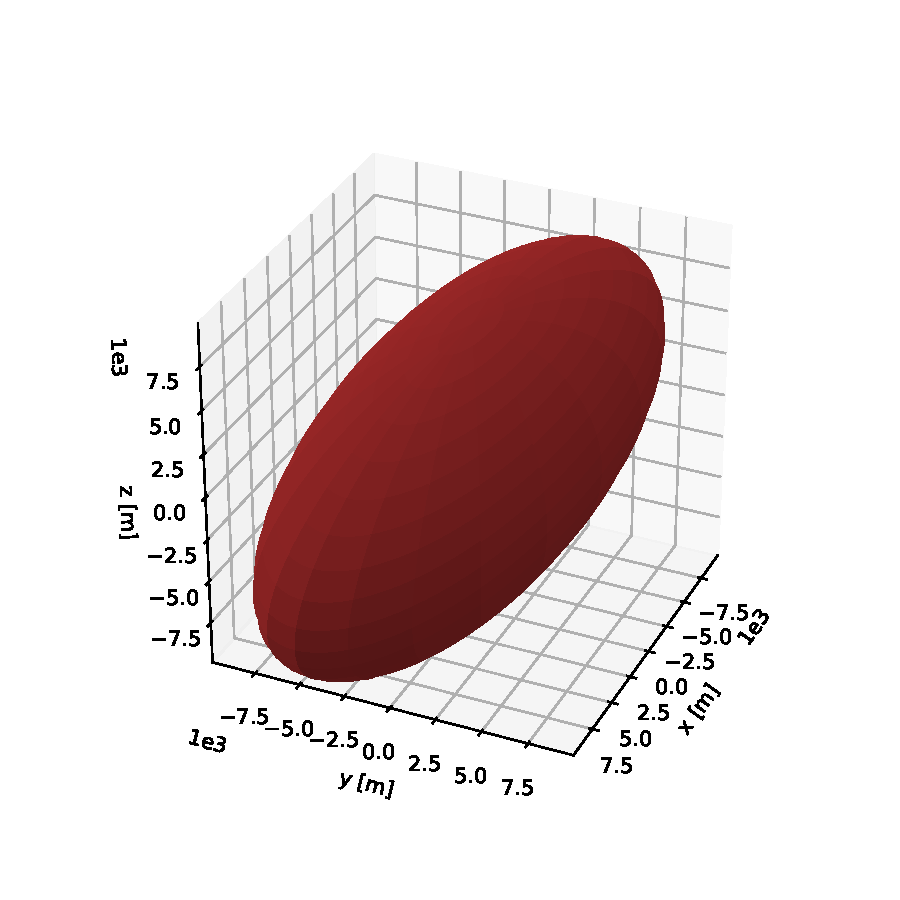
\includegraphics[width=\textwidth, height=0.27\textheight, keepaspectratio=true]{cde.pdf}
\caption{Triaxial ellipsoid model with semi-major axes $\alpha=20$ km, $\beta=7$ km, $\gamma=7$ km.}
\label{fig:cde}
\end{figure}
\FloatBarrier
%%%
For a given point $(x, y, z)$ in space around the \gls{CDE}, the only unknown in \Cref{eqn:cubicPolynomial} is $\lambda$ which is solved for using the standard Cardano's formula (see \cite{cubic_formula}). Now for the given ellipsoid, the equation for the family of confocal quadratic surfaces is given as follows \parencite{ellipsoid_potential_model}:
%%%
\begin{align}
    \frac{x^2}{\alpha^2 + u} + \frac{y^2}{\beta^2 + u} + \frac{z^2}{\gamma^2 + u} &= 1
    \label{eqn:confocal_quadrics}
\end{align}
%%%
where $u$ is a real-valued parameter whose value defines the type of the confocal quadratic surface. \Cref{eqn:confocal_quadrics} is a cubic polynomial in $u$ and can be solved to obtain three unequal real roots - $u_1, u_2, u_3$, such that the following relation holds true \parencite{ellipsoid_potential_model}:
%%%
\begin{align}
    -\alpha^2 < u_3 < -\beta^2 < u_2 < -\gamma^2 < u_1 < +\infty
    \label{eqn:confocal_quadrics_all_real_roots}
\end{align}
%%%
where $u_1$ is the maximum real root possible and at that value, \Cref{eqn:confocal_quadrics} defines another ellipsoid which is confocal to the original one defined by the semi-major axes $\rightarrow$ $\alpha, \beta, \gamma$ \parencite{ellipsoid_potential_model}. Thus, the value of $\lambda$ in \Cref{eqn:ellipsoid_potential_short_form} conforms to a confocal ellipsoid for a given point external to the original ellipsoid (which in turn is modeling the asteroid).
% The standard definition of gravity potential at a point is defined as the work required to move that point from infinity to the location of the point in question and in \Cref{eqn:ellipsoid_potential_short_form}, this is being done by moving through a family of confocal ellipsoids.
%
\newline\newline
%
The potential defined by \Cref{eqn:ellipsoid_potential_short_form} appears to have a complicated computational process due to its integral form. However, the integral can be split into multiple parts such that each can be solved with the help of standard functions called \textit{Carlson's Elliptic Integrals} \parencite{carlsonEllipticIntegral}. Software routines for these integrals exist in several computing languages which, for our case, helps in computing the \gls{CDE} gravity potential. The integral defined in \Cref{eqn:ellipsoid_potential_short_form,eqn:ellipsoid_potential_phi,eqn:ellipsoid_potential_delta} is restated in its complete form as follows:
%%%
\begin{align}
    U(\bvector{r}) &= -\frac{3\mu}{4} \int_{\lambda(\bvector{r})}^{\infty} \left(\frac{x^2}{\alpha^2 + u} + \frac{y^2}{\beta^2 + u} + \frac{z^2}{\gamma^2 + u} - 1\right) \frac{du}{\sqrt{(\alpha^2 + u)(\beta^2 + u)(\gamma^2 + u)}}
    \label{eqn:ellipsoid_potential_long_form}
\end{align}
%%%
\Cref{eqn:ellipsoid_potential_long_form} can be split into 4 parts which are stated as follows:
%%%
\begin{align}
    U_1 &= -\frac{\mu}{2} \cdotp \frac{3}{2} \int_{\lambda}^{\infty} \frac{x^2}{(\alpha^2 + u)^{3/2}(\beta^2 + u)^{1/2}(\gamma^2 + u)^{1/2}} du
    \label{eqn:ellipsoid_potential_split_1}\\
    U_2 &= -\frac{\mu}{2} \cdotp \frac{3}{2} \int_{\lambda}^{\infty} \frac{y^2}{(\alpha^2 + u)^{1/2}(\beta^2 + u)^{3/2}(\gamma^2 + u)^{1/2}} du
    \label{eqn:ellipsoid_potential_split_2}\\
    U_3 &= -\frac{\mu}{2} \cdotp \frac{3}{2} \int_{\lambda}^{\infty} \frac{z^2}{(\alpha^2 + u)^{1/2}(\beta^2 + u)^{1/2}(\gamma^2 + u)^{3/2}} du
    \label{eqn:ellipsoid_potential_split_3}\\
    U_4 &= +\frac{\mu}{2} \cdotp \frac{3}{2} \int_{\lambda}^{\infty} \frac{du}{(\alpha^2 + u)^{1/2}(\beta^2 + u)^{1/2}(\gamma^2 + u)^{1/2}}
    \label{eqn:ellipsoid_potential_split_4}
\end{align}
%%%
where $\lambda{(\bvector{r})}$ is simply written as $\lambda$ for brevity. Thus, the \gls{CDE} potential is given as $U = U_1 + U_2 + U_3 + U_4$. We make the following substitution for \Cref{eqn:ellipsoid_potential_split_1,eqn:ellipsoid_potential_split_2,eqn:ellipsoid_potential_split_3,eqn:ellipsoid_potential_split_4}:
%%%
\begin{align}
    u &= v + \lambda
    \label{eqn:ellipsoidal_potential_substitution_1} \\
    du &= dv
    \label{eqn:ellipsoidal_potential_substitution_2} \\
    u &= \lambda \text{; } v = 0
    \label{eqn:ellipsoidal_potential_substitution_3} \\
    u &= \infty \text{; } v = \infty
    \label{eqn:ellipsoidal_potential_substitution_4}
\end{align}
%%%
With these substitutions, \Cref{eqn:ellipsoid_potential_split_1}, for example, can now be re-written as follows:
%%%
\begin{align}
    U_1 &= -\frac{\mu x^2}{2} \left[\frac{3}{2} \int_{0}^{\infty} \frac{dv}{((\alpha^2 + \lambda) + v)^{3/2}((\beta^2 + \lambda) + v)^{1/2}((\gamma^2 + \lambda) + v)^{1/2}}\right]
    \label{eqn:ellipsoid_potential_split_1_mod} \\
    &= -\frac{\mu x^2}{2} R_D(\beta^2 + \lambda, \gamma^2 + \lambda, \alpha^2 + \lambda)
    \label{eqn:ellipsoid_potential_split_1_carlson}
\end{align}
%%%
In \Cref{eqn:ellipsoid_potential_split_1_mod}, the expression within the square braces conforms to the standard elliptic integral function $R_D$ as defined by \cite{carlsonEllipticIntegral} and is given as follows:
%%%
\begin{align}
    R_D(x, y, z) &= \frac{3}{2} \int_0^{\infty} \frac{dt}{(t+x)^{1/2}(t+y)^{1/2}(t+z)^{3/2}}
    \label{eqn:carlson_RD}
\end{align}
%%%
Similarly, \Cref{eqn:ellipsoid_potential_split_2,eqn:ellipsoid_potential_split_3} can be re-written using the standard elliptic integral function $R_D$ as follows:
%%%
\begin{align}
    U_2 &= -\frac{\mu y^2}{2} R_D(\alpha^2 + \lambda, \gamma^2 + \lambda, \beta^2 + \lambda)
    \label{eqn:ellipsoid_potential_split_2_carlson} \\
    U_3 &= -\frac{\mu z^2}{2} R_D(\alpha^2 + \lambda, \beta^2 + \lambda, \gamma^2 + \lambda)
    \label{eqn:ellipsoid_potential_split_3_carlson}
\end{align}
%%%
For \Cref{eqn:ellipsoid_potential_split_4}, we use another standard elliptic integral function as defined by \cite{carlsonEllipticIntegral}:
%%%
\begin{align}
    R_F(x, y, z) &= \frac{1}{2} \int_0^\infty \frac{dt}{(t+x)^{1/2}(t+y)^{1/2}(t+z)^{1/2}}
    \label{eqn:carlson_RF}
\end{align}
%%%
using which, \Cref{eqn:ellipsoid_potential_split_4} is re-written as follows:
%%%
\begin{align}
    U_4 &= \frac{3\mu}{2} R_F(\alpha^2 + \lambda, \beta^2 + \lambda, \gamma^2 + \lambda)
    \label{eqn:ellipsoid_potential_split_4_carlson}
\end{align}
%%%
Thus, to calculate the \gls{CDE} gravity potential $U$ at any given point $(x,y,z)$ external to the ellipsoid, we first calculate the corresponding value of $\lambda$ from \Cref{eqn:cubicPolynomial} and then substitute this value into \Cref{eqn:ellipsoid_potential_split_1_carlson,eqn:ellipsoid_potential_split_2_carlson,eqn:ellipsoid_potential_split_3_carlson,eqn:ellipsoid_potential_split_4_carlson}, the sum of which is the final potential value.
%
\newline\newline
%
The gravitational acceleration components are obtained by taking a partial derivatives of the potential equation given in \Cref{eqn:ellipsoid_potential_long_form} \parencite{scheeresBook}:
%%%
\begin{align}
    U_x &= -\frac{3\mu x}{2} \int_{\lambda(\bvector{r})}^{\infty} \frac{du}{(\alpha^2 + u) \Delta u}
    \label{eqn:grav_acc_x} \\
    U_y &= -\frac{3\mu y}{2} \int_{\lambda(\bvector{r})}^{\infty} \frac{du}{(\beta^2 + u) \Delta u}
    \label{eqn:grav_acc_y} \\
    U_z &= -\frac{3\mu z}{2} \int_{\lambda(\bvector{r})}^{\infty} \frac{du}{(\gamma^2 + u) \Delta u}
    \label{eqn:grav_acc_z}
\end{align}
%%%
where $(U_x, U_y, U_z)$ are the gravitational acceleration terms and all other terms have the same definition as explained before for the \gls{CDE} potential term. Just like with the gravity potential, the acceleration terms can be reduced to standard Carlson's elliptic integrals by using the same substitution parameters as defined in \Cref{eqn:ellipsoidal_potential_substitution_1,eqn:ellipsoidal_potential_substitution_2,eqn:ellipsoidal_potential_substitution_3,eqn:ellipsoidal_potential_substitution_4}. After substitution, for example, the x-component of the acceleration term is written as follows:
%%%
\begin{align}
    U_x &= -\frac{-3\mu x}{2} \int_{0}^{\infty} \frac{dv}{(\alpha^2 + v + \lambda)\sqrt{(\alpha^2 + v + \lambda)(\beta^2 + v + \lambda)(\gamma^2 + v + \lambda)}} \\
    &= -\mu x \left[\frac{3}{2} \int_0^\infty \frac{dv}{((\alpha^2 + \lambda) + v)^{3/2} ((\beta^2 + \lambda) + v)^{1/2} ((\gamma^2 + \lambda) + v)^{1/2}} \right] \\
    &= -\mu x \cdotp R_D((\beta^2 + \lambda), (\gamma^2 + \lambda), (\alpha^2 + \lambda))
    \label{eqn:grav_acc_x_carlson}
\end{align}
%%%
Similarly, the other components of the gravitational acceleration (defined in the \gls{ARF}) can be written as follows:
%%%
\begin{align}
    U_y &= -\mu y \cdotp R_D((\alpha^2 + \lambda), (\gamma^2 + \lambda), (\beta^2 + \lambda))
    \label{eqn:grav_acc_y_carlson} \\
    U_z &= -\mu z \cdotp R_D((\alpha^2 + \lambda), (\beta^2 + \lambda), (\gamma^2 + \lambda))
    \label{eqn:grav_acc_z_carlson}
\end{align}
%%%
For any point $(x,y,z)$ outside of the \gls{CDE}, we calculate the value for $\lambda$ first by solving \Cref{eqn:cubicPolynomial} and then substitute it into \Cref{eqn:grav_acc_x_carlson,eqn:grav_acc_y_carlson,eqn:grav_acc_z_carlson} to get the acceleration components in the \gls{ARF}.

\section{Solar Perturbations}
\label{sec:solar_perturbations}
The dominant force acting on an orbiting particle in the vicinity of an asteroid is from its gravity field. However, perturbations, both gravitational and non-gravitational, can be significant especially when the particle is further away from the asteroid \parencite{scheeresBook}. The two most significant sources of perturbations are from the Sun and we will be discussing them briefly in this section.

\subsection{Solar Third-Body Effect (STBE)}
\label{subsec:stbe}
We consider a simple two-body problem, wherein the asteroid has a circular, Heliocentric orbit in the Ecliptic plane. This is a reasonable approximation, as mentioned earlier in \Cref{sec:assumptions}, since several asteroids have been observed to have circular orbits around the Sun with near-zero inclinations. The gravitational effect of the Sun on the motion of regolith (henceforth \gls{STBE}) around the asteroid is not modeled through a three-body problem because the order of magnitude of the perturbing acceleration is extremely small relative to the gravitational acceleration of the asteroid (atleast 5 orders of magnitude smaller in the vicinity of a sample asteroid at 1 AU from the Sun) and hence it is sufficient to model it as an external perturbing acceleration.
%
\newline\newline
%
The absolute gravitational acceleration, due to the Sun, experienced by a particle (of mass negligible compared to that of the Sun) in orbital motion around the asteroid is given as \parencite{scheeresBook}:
%%%
\begin{align}
    \bv{a}_{abs, p} &= -\frac{\mu_S}{|\bv{r} - \bv{d}|^3} (\bv{r} - \bv{d})
    \label{eqn:stbe_particle_abs_acc}
\end{align}
%%%
where $\mu_S$ is the gravitational parameter of the Sun; \bvt{r} and \bvt{d} are the position vectors of the orbiting particle and the Sun, respectively, from the asteroid's centre of mass, defined in the \gls{AIF}. In \Cref{eqn:stbe_particle_abs_acc}, the Sun is viewed to be orbiting the asteroid, instead of the other way around. This is just a change in perspective and is done to keep all distance vector definitions originating from the centre of mass of the asteroid \parencite{scheeresBook}. The orientation of the position vectors is shown in \Cref{fig:stbe_inertialFrame}.
%%%
\begin{figure}[htb]
\centering
\captionsetup{justification=centering}
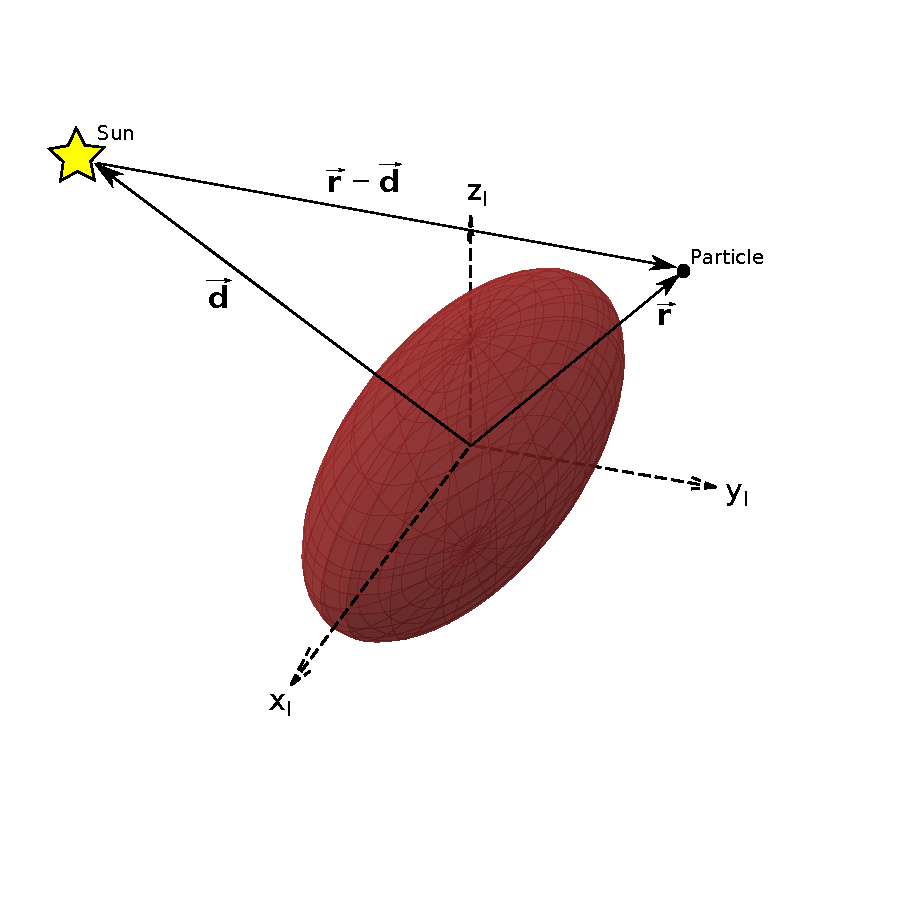
\includegraphics[width=\textwidth, height=0.35\textheight, keepaspectratio=true]{stbe_bodyframe_edit_2.pdf}
\caption{A schematic representing the orientation of position vectors of the Sun and the orbiting particle/regolith around the asteroid, in the \gls{AIF}. Diagram is not to scale and the rotation state of asteroid is such that the \gls{ARF} and \gls{AIF} are coinciding.}
\label{fig:stbe_inertialFrame}
\end{figure}
\FloatBarrier
%%%
Now the absolute gravitational acceleration, due to the Sun, experienced by the asteroid is given as follows \parencite{scheeresBook}:
%%%
\begin{align}
    \bv{a}_{abs, a} &= +\frac{\mu_S}{|\bv{d}|^3} (\bv{d})
    \label{eqn:stbe_asteroid_abs_acc}
\end{align}
%%%
where the definition of all variables is the same as that for \Cref{eqn:stbe_particle_abs_acc}. Thus, the perturbing acceleration acting on the particle due to the \gls{STBE} is the difference between the absolute accelerations experienced by the particle (\Cref{eqn:stbe_particle_abs_acc}) and the asteroid (\Cref{eqn:stbe_asteroid_abs_acc}) \parencite{scheeresBook}:
%%%
\begin{align}
    \bv{a}_{STBE} &= -\mu_S \left[ \frac{(\bv{r} - \bv{d})}{|\bv{r} - \bv{d}|^3} + \frac{\bv{d}}{|\bv{d}|^3} \right]
    \label{eqn:stbe_acc}
\end{align}
%%%
The perturbing acceleration in \Cref{eqn:stbe_acc} can be re-written in the form of a potential as follows \parencite{scheeresBook}:
%%%
\begin{align}
    \mathcal{R}_{STBE} &= \mu_S \left[\frac{1}{|\bv{r} - \bv{d}|} - \frac{\bv{d}\cdotp\bv{r}}{|\bv{d}|^3} \right]
    \label{eqn:stbe_potential} \\
    \bv{a}_{STBE} &= \frac{\delta \mathcal{R}_{STBE}}{\delta\bv{r}}
\end{align}
%%%
In \Cref{eqn:stbe_acc}, we can directly substitute the position vectors as defined in \gls{ARF} such that the acceleration term obtained is also in the \gls{ARF}. This is possible because the position magnitude terms would remain the same in either of the reference frames. Also, the rotation matrix $\phi_I^B$ multiplied either outside the square bracket or inside, in \Cref{eqn:stbe_acc}, with the two numerator terms would ultimately give the same result.
%%%
\begin{align}
    \ddot{\bv{d}} &= -\frac{\mu_S}{|\bv{d}|^3} (\bv{d})
    \label{eqn:sun_around_asteroid}
\end{align}
%%%
The apparent position of the Sun, relative to the asteroid, can be obtained in two ways. We could either numerically integrate the second order differential equation for the standard two-body problem as stated in \Cref{eqn:sun_around_asteroid} or solve, what is historically known as, the \textit{Kepler's problem}. We use the latter since the apparent position of the Sun can be obtained for any time value directly by using the Kepler's problem algorithm as stated by \cite{chobotovBook}. Although the Kepler's problem algorithm is not completely analytical and uses a numerical iteration method to solve for the true anomaly, it is relatively easier to use within the simulator than employing a numerical integrator to propagate the position from an initial condition for every time value. The algorithm for solving the Kepler's problem is not stated here for brevity; A detailed explanation for it is given by \cite{chobotovBook}.

\subsection{Solar Radiation Pressure (SRP)}
\label{subsec:srp}
With the heliocentric orbit of the asteroid, in addition to the \gls{STBE}, is a non-gravitational source of perturbation acting on an asteroid-orbiting particle, called \gls{SRP}. Momentum transfer takes place from the Solar photons that strike and recoil from the surface of the particle, which thus perturbs the orbital motion \parencite{scheeresBook}.
%
\newline\newline
%
We use a model for \gls{SRP} that assumes that the particle always presents a constant area to the impinging Solar photons and the area is perpendicular to the Sun-line. The total momentum transfer is modeled as Solar irradiance and reflection and the acceleration due to \gls{SRP} thus acts in a direction away from and along the Sun-line \parencite{scheeresBook}. This acceleration is given as follows:
%%%
\begin{align}
    \bv{a}_{SRP} &= -(1 + \rho) P_0 \cdotp \frac{A}{M} \cdotp \frac{(\bv{d} - \bv{r})}{|\bv{d} - \bv{r}|^3}
    \label{eqn:srp_acc}
\end{align}
%%%
where $\rho$ is the albedo of the particle; $P_0$ is a Solar constant whose value is $1.0\times10^{17}$ \si{\kilogram \metre \per \second \squared}; $A/M$ is the area-to-mass ratio of the particle and area refers to the cross-sectional area of the particle on which the Solar photons are striking; \bvt{d} is the distance vector from the asteroid to the Sun and \bvt{r} is the distance vector from the asteroid to the orbiting particle \parencite{scheeresBook}. The \gls{SRP} perturbing acceleration can be re-stated in terms of a perturbing potential as follows:
%%%
\begin{align}
    \mathcal{R}_{SRP} &= -(1 + \rho) P_0 \cdotp \frac{A}{M} \left[\frac{1}{|\bv{d}-\bv{r}|}\right]
    \label{eqn:srp_potential} \\
    \bv{a}_{SRP} &= \frac{\delta \mathcal{R}_{SRP}}{\delta \bv{r}}
\end{align}
%%%

\section{Perturbed Two-Body Problem}
\label{sec:2BP}
We have discussed the gravity potential and the perturbations model to be used for our system, and now we'll present the \gls{EOM} that govern the motion of the lofted particle. Note that the \gls{CDE} potential model is defined for a body-fixed frame inherently which means the accelerations that we get out of it are directly defined for the \gls{ARF} frame. The same applies for the \gls{STBE} and \gls{SRP} perturbing accelerations. This is why we define the equations of motion too in the \gls{ARF} frame and transform the propagated state to the \gls{AIF} frame post-simulation.
%
\newline\newline
%
We use a Lagrangian approach to derive the \gls{EOM} because once the Lagrangian is formed, it becomes relatively easy to re-write the \gls{EOM} for a different frame of reference or a different set of coordinates by substituting the relevant transformation equations in the Lagrangian. It is formed as $L=T+\mathcal{U}$, where $T$ is the specific kinetic energy and $\mathcal{U}$ is the full potential of the system and they are given as follows \parencite{scheeresBook}:
%%%
\begin{align}
    T &= \frac{1}{2} \dot{\bv{r}}_I \cdotp \dot{\bv{r}}_I
    \label{eqn:lagrangian_kinetic_energy} \\
    \mathcal{U} &= U + \mathcal{R}_{STBE} + \mathcal{R}_{SRP}
    \label{lagrangian_potential}
\end{align}
%%%
where $\bv{r}_I$ is the position vector of the particle from the asteroid to the orbiting particle and expressed in the \gls{AIF}; $U$ is the \gls{CDE} gravity potential; $\mathcal{R}_{STBE}$ and $\mathcal{R}_{SRP}$ are the perturbing potentials for the Sun's third-body effect and radiation pressure respectively. The \gls{EOM} is then obtained from the following \parencite{scheeresBook}:
%%%
\begin{align}
    \frac{d}{dt} \left(\frac{\delta L}{\delta \dot{x}_i}\right) &= \frac{\delta L}{\delta x_i}
    \label{eqn:lagrange_general_form}
\end{align}
%%%
where $(x_i, \dot{x}_i)$ are the position and velocity vector components. We will now evaluate \Cref{eqn:lagrange_general_form} for our particular case by first re-stating the Lagrangian with vectors expressed in the \gls{ARF}. With $(\bv{q}, \dot{\bv{q}})$ denoting the \gls{ARF} position and velocity vectors respectively, the position vector in the \gls{AIF} is related to the \gls{ARF} as $\bv{r} = \phi_B^I \bv{q}$ and the velocity is related as $\dot{\bv{r}} = \phi_I^B \cdotp (\dot{\bv{q}} + \bv{\omega} \times \bv{q})$. With these definitions, the Lagrangian is re-written as follows:
%%%
\begin{align}
    L &= (\dot{\bv{q}} + \bv{\omega} \times \bv{q}) \cdotp (\dot{\bv{q}} + \bv{\omega} \times \bv{q}) + \mathcal{U}(\bv{q})
    \label{eqn:lagrange_arf}
\end{align}
%%%
where the transformation matrix $\phi_B^I$ preserves \footnote{For two vectors \bvt{u} and \bvt{v}, and an orthogonal matrix $Q$, $\bv{u} \cdotp \bv{v} = (Q\bv{u}) \cdotp (Q\bv{v})$} the dot product, as it is orthogonal, and hence is excluded from the equation. The derivative on the right hand side of \Cref{eqn:lagrange_general_form}, directly in vector form, is evaluated as follows:
%%%
\begin{align}
    \frac{\delta L}{\delta \bv{q}} &= \frac{1}{2} \left[ 2 \cdotp (\dot{\bv{q}} + \bv{w} \times \bv{q}) \cdotp (\bv{\omega} \times \bv{1} + \bv{q} \times {\bv{0}}) \right] + \frac{\delta \mathcal{U}}{\delta \bv{q}} \\
    &= \dot{\bv{q}} \cdotp (\bv{\omega} \times \bv{1}) + (\bv{\omega} \times \bv{q}) \cdotp (\bv{\omega} \times \bv{1}) + \frac{\delta \mathcal{U}}{\delta \bv{q}} \\
    &= (\dot{\bv{q}} \times \bv{\omega}) \cdotp \bv{1} + \bv{1} \cdotp ((\bv{\omega} \times \bv{q}) \times \bv{\omega}) + \frac{\delta \mathcal{U}}{\delta \bv{q}} \\
    &= -(\bv{\omega} \times \dot{\bv{q}}) - (\bv{\omega} \times (\bv{\omega} \times \bv{q})) + \frac{\delta \mathcal{U}}{\delta \bv{q}}
    \label{eqn:lagrangian_RHS}
\end{align}
%%%
where \bvt{1} and \bvt{0} are vectors of ones and zeros respectively and all other terms have been defined previously. The left hand side of \Cref{eqn:lagrange_general_form} is evaluated as follows:
%%%
\begin{align}
    \frac{\delta L}{\delta \dot{\bv{q}}} &= \dot{\bv{q}} + (\bv{\omega} \times \bv{q}) \\
    \frac{d}{dt}\left( \frac{\delta L}{\delta \dot{\bv{q}}} \right) &= \ddot{\bv{q}} + \bv{\omega} \times \dot{\bv{q}}
    \label{eqn:lagrangian_LHS}
\end{align}
%%%
Thus, by substituting \Cref{eqn:lagrangian_LHS,eqn:lagrangian_RHS} into \Cref{eqn:lagrange_general_form}, we get the final equations of motion as follows:
%%%
\begin{align}
    \ddot{\bv{q}} + 2 \cdotp \bv{\omega} \times \dot{\bv{q}} + (\bv{\omega} \times (\bv{\omega} \times \bv{q})) &= \frac{\delta \mathcal{U}}{\delta \bv{q}} \\
    &= \frac{\delta U(\bv{q})}{\delta \bv{q}} + \frac{\delta \mathcal{R}_{STBE}}{\delta \bv{q}} + \frac{\delta \mathcal{R}_{SRP}}{\delta \bv{q}}
    \label{eqn:lagrangian_potential_eval} \\
    \ddot{\bv{q}} + 2 \cdotp \bv{\omega} \times \dot{\bv{q}} + (\bv{\omega} \times (\bv{\omega} \times \bv{q})) &= \frac{\delta U(\bv{q})}{\delta \bv{q}} + \bv{a}_{STBE} + \bv{a}_{SRP}
    \label{eqn:p2bp}
\end{align}
%%%
In \Cref{eqn:lagrangian_potential_eval}, the first term denotes the acceleration due to gravity, and the second and the third term denote the perturbing accelerations. \Cref{eqn:p2bp} is thus the final equation of motion used in this thesis.

\section{Particle Initial Conditions}
\label{sec:init_conditions}
The \gls{EOM} established in the previous section are difficult to solve analytically and hence we make use of a numerical integrator to propagate the state vector of an orbiting particle in time. To do this, we need to establish robust methods for providing initial conditions. These initial conditions basically form the state vector with which the particle is lofted from the surface of an asteroid.

\subsection{Launch Location}
\label{subsec:launch_location}
This section will present a method to efficiently calculate the launch location of a particle, in the form of a Cartesian position vector from the centre of the asteroid. The formulation is such that the resulting position vector will always point to a location on the surface of the asteroid.
%
\newline\newline
%
Consider the equation for the ellipsoid given as follows:
%%%
\begin{align}
    \frac{x^2}{\alpha^2} + \frac{y^2}{\beta^2} + \frac{z^2}{\gamma^2} &= 1
    \label{eqn:launch_loc_ellipsoid_eqn_cartesian}
\end{align}
%%%
where $(x,y,z)$ is the coordinate of any point on the surface. An alternate way of writing \Cref{eqn:launch_loc_ellipsoid_eqn_cartesian}, in vector format, is given as follows:
%%%
\begin{align}
    \bv{r}.E.\bv{r} &= 1
    \label{eqn:launch_loc_ellipsoid_eqn_vectorForm} \\
    E &=
    \begin{bmatrix}
        1/\alpha^2 & 0 & 0 \\
        0 & 1/\beta^2 & 0 \\
        0 & 0 & 1/\gamma^2
    \end{bmatrix}
\end{align}
%%%
where \bvt{r} is a general position vector expressed in the \gls{ARF} and ($\alpha, \beta, \gamma$) are the semi-major axes of the triaxial ellipsoid model of the asteroid. Continuing with \Cref{eqn:launch_loc_ellipsoid_eqn_vectorForm}:
%%%
\begin{align}
    \bv{r}.\bv{r} &= \frac{1}{E} \\
    r^2 &= \frac{1}{\buvec{u}.E.\buvec{u}}
    \label{eqn:launch_loc_r_square}
\end{align}
%%%
where $\buvec{u}$ is a unit vector expressed in \gls{ARF}, pointing in the direction of the launch location from the asteroid's centre, with components $(u_x, u_y, u_z)$. The unit vector can be stated in terms of the latitude $(\delta)$ and longitude $(\lambda)$ of the launch point as follows:
%%%
\begin{align}
    \buvec{u} &= \cos\delta \cos\lambda \buvec{x} + \cos\delta \sin\lambda \buvec{y} + \sin\delta \buvec{z}
\end{align}
%%%
where $(\buvec{x},\buvec{y},\buvec{z})$ are the basis vectors forming the \gls{ARF}. Thus, \Cref{eqn:launch_loc_r_square} can be written as:
%%%
\begin{align}
    r^2 &= \frac{1}{ (u_x^2/\alpha^2) + (u_y^2/\beta^2) + (u_z^2/\gamma^2) }
    \label{eqn:launch_loc_r_square_expanded}
\end{align}
%%%
The final position vector to the launch location, from the origin of \gls{ARF} or the asteroid's centre, is given as follows:
%%%
\begin{align}
    \bv{r}_s &= r\buvec{u}
    \label{eqn:launch_vector}
\end{align}
%%%
where $r$ is obtained from \Cref{eqn:launch_loc_r_square_expanded}. Thus, just by specifying the latitude and longitude of any desired launch point, the position vector to it is obtained. This, thus, acts as the initial position state of the particle.

\subsection{Launch Velocity}
\label{subsec:launch_velocity}
Once we know the position of the particle, we need to provide an initial velocity to launch it into an orbit around the asteroid. But this has to do much more than just providing a velocity magnitude. The velocity magnitude is accompanied by a launch direction which is defined by two angles, namely, Launch Azimuth ($\eta$) and Launch Declination ($\chi$).
%
\newline\newline
%
These angles can be understood as follows. Suppose you are standing on the surface of an asteroid and you throw a ball. Now the ball will be associated with a velocity vector and if we take the projection of this vector onto the local surface, then the angle between this projection and the local direction to the North pole of the asteroid is defined as the launch azimuth. The angle that the velocity vector itself makes with the local normal is then defined as the launch declination. By keeping a constant angle of declination and varying the launch azimuth from \SI{0}{\degree} to \SI{360}{\degree}, we can create a cone of particles, thus replicating how impact ejecta would launch out. An example of this is given in \Cref{fig:longest_edge_velocity_vector_cone}.
%%%
\begin{figure}[htb]
\centering
\captionsetup{justification=centering}
\subfloat[]{
    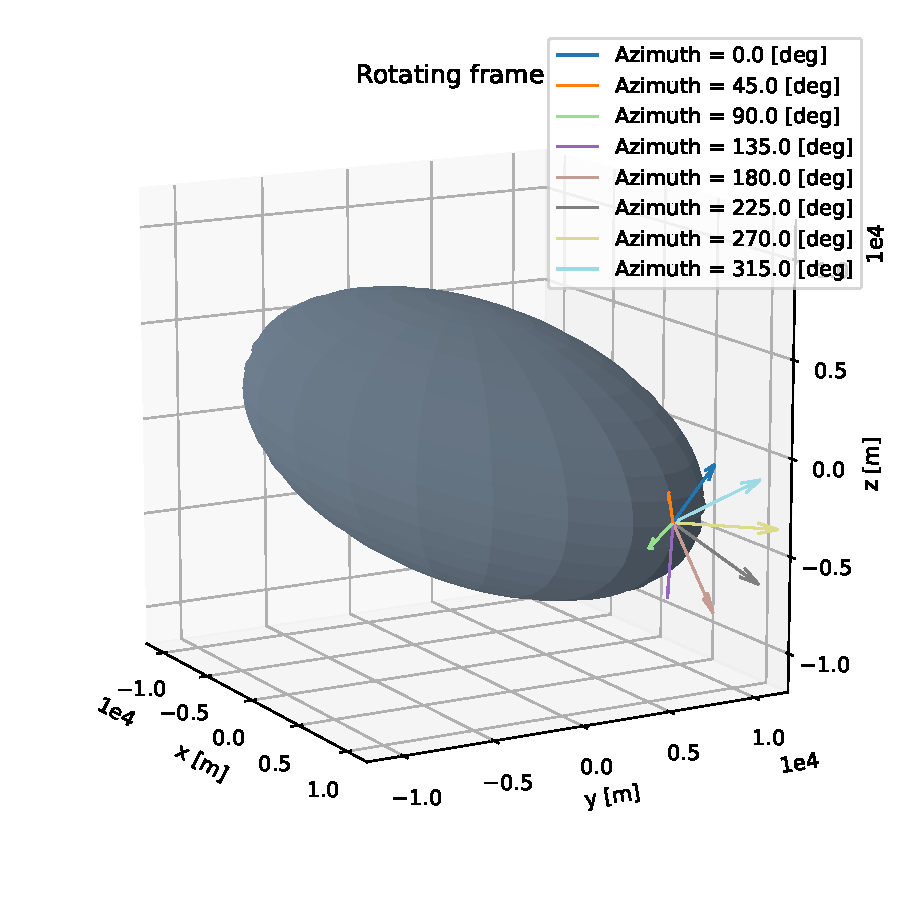
\includegraphics[width=\textwidth, height=0.5\textheight, keepaspectratio=true]{longest_edge_ARF_velocity_vectors_cone.pdf}
    \label{fig:longestEdge_velocity_vector_cone_1}
}

\subfloat[]{
    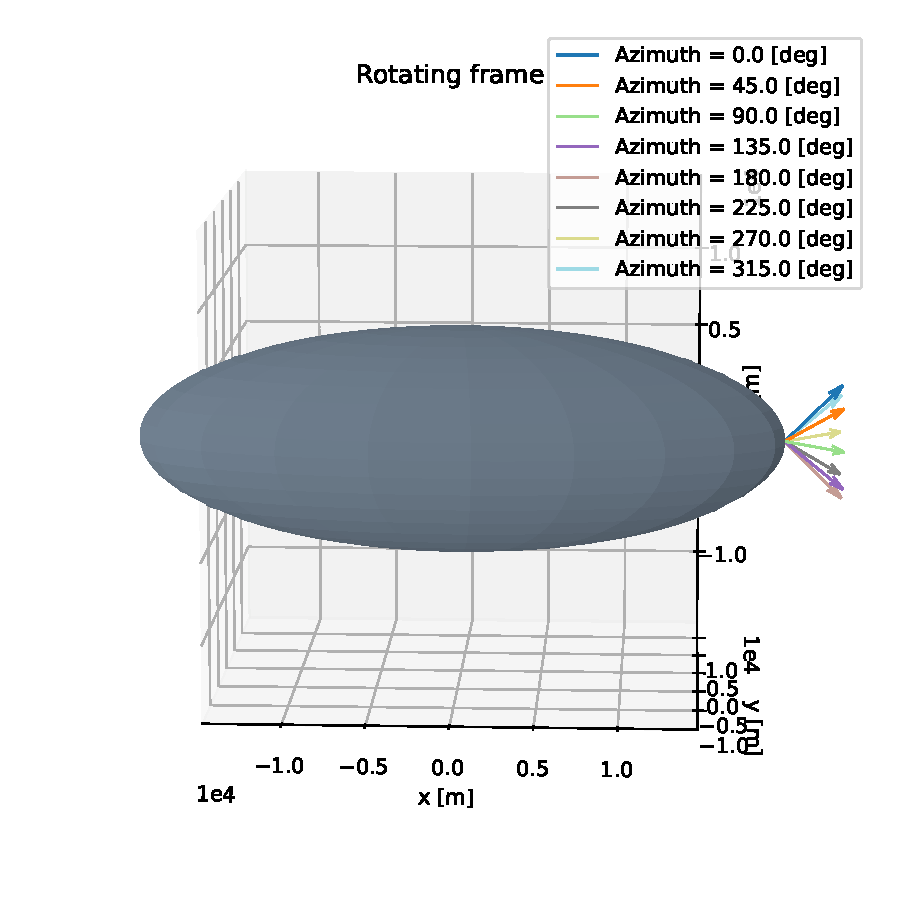
\includegraphics[width=\textwidth, height=0.5\textheight, keepaspectratio=true]{velocity_vector_ARF_lateral_view.pdf}
    \label{fig:longestEdge_velocity_vector_cone_2}
}
\caption{Various velocity vectors depicted at the longest edge of the ellipsoid shaped asteroid i.e. for a launch location longitude and latitude of \SI{0}{\degree}. \protect\Cref{fig:longestEdge_velocity_vector_cone_1} depicts the front view of multiple velocity vectors spaced at \SI{45}{\degree} azimuth from each other and at a constant declination of \SI{45}{\degree}. All vectors are expressed in the rotating frame or the \gls{ARF}. \protect\Cref{fig:longestEdge_velocity_vector_cone_2} depicts the lateral view of the same velocity vectors.}
\label{fig:longest_edge_velocity_vector_cone}
\end{figure}
\FloatBarrier
%%%
We will now discuss how the velocity vectors are formed in practice. Consider the equation for a triaxial ellipsoid given in \Cref{eqn:launch_loc_ellipsoid_eqn_cartesian}. Now for any given point $(x,y,z)$ on the surface of the ellipsoid, the normal vector ($\bv{n}$) (and subsequently the unit normal vector ($\buvec{n}$)) to it is found by taking the gradient of \Cref{eqn:launch_loc_ellipsoid_eqn_cartesian}:
%%%
\begin{align}
    \bv{n} &= \frac{2x}{\alpha^2}\buvec{i} + \frac{2y}{\beta^2}\buvec{j} + \frac{2z}{\gamma^2}\buvec{k}
    \label{eqn:surface_normal_vector} \\
    \buvec{n} &= \frac{\bv{n}}{|\bv{n}|}
    \label{eqn:unit_normal}
\end{align}
%%%
where both \bvt{n} and $\buvec{n}$ are expressed in the \gls{ARF}, whose basis vectors are denoted here as ($\buv{i},\buv{j},\buv{k}$). Note that since the body in question is not a sphere, the normal vector at the launch location and the radial unit vector $\buv{R}$ (from the centre of the ellipsoid to the launch location) may not always coincide. Now that we know the unit normal vector to the launch location, we need to find the local North direction. This is done by performing the following calculations successively:
%%%
\begin{align}
    \buv{R} &= \frac{\bv{r}_s}{|\bv{r}_s|} \\
    \buv{T} &= \frac{\buv{R} \times \buv{k}}{|\buv{R} \times \buv{k}|} \\
    \buv{x} &= \frac{\buv{T} \times \buv{n}}{|\buv{T} \times \buv{n}|} \\
    \label{eqn:surface_frame_xBasis}
\end{align}
%%%
where $\bv{r}_s$ is the position vector to the launch location from the centre of the asteroid; $\buv{T}$ is the tangential unit vector (tangential to the local surface at the local point); $\buv{x}$ is the unit vector that is pointing towards the local North. This formulation works for any point on the surface of the asteroid to give the local North's direction except for the two poles and as such an alternative definition for them has to be used which will be defined later. Note that all the unit vectors discussed so far are expressed in the \gls{ARF}.
%
\newline\newline
%
$\buv{x}$ is also viewed as the x-axis basis vector for a frame of reference fixed and centered at the launch location. This frame of reference is termed as the \gls{SF}. Note that the \gls{SF} is not used to define the orbital motion of the regolith and hence it is not one of the standard reference frames. This is why it was not mentioned in \Cref{sec:reference_frames} and is only defined here since it's use is only for obtaining the velocity vector. The z-axis of \gls{SF} is defined in the direction of the unit normal vector at the launch location and the y-axis is obtained by following the right-hand rule to form the orthogonal frame. The \gls{SF} is shown in \Cref{fig:surface_frame}.
%
\newline\newline
%
Note that the basis vectors of the \gls{SF} are expressed in the \gls{ARF} and thus their components are defined as follows:
%%%
\begin{align}
    \buv{x} &= x_1\buv{i} + x_2\buv{j} + x_3\buv{k}
    \label{eqn:sf_xbasis_exp} \\
    \buv{y} &= y_1\buv{i} + y_2\buv{j} + y_3\buv{k}
    \label{eqn:sf_ybasis_exp} \\
    \buv{z} &= z_1\buv{i} + z_2\buv{j} + z_3\buv{k}
    \label{eqn:sf_zbasis_exp}
\end{align}
%%%
Then the velocity vector components in \gls{ARF} are obtained as follows:
%%%
\begin{align}
    v_x &= V . \left[ x_1 \cos\eta \sin\chi + y_1 \sin\eta \sin\chi + z_1 \cos\chi \right]
    \label{eqn:xVelocity} \\
    v_y &= V . \left[ x_2 \cos\eta \sin\chi + y_2 \sin\eta \sin\chi + z_2 \cos\chi \right]
    \label{eqn:yVelocity} \\
    v_z &= V . \left[ x_3 \cos\eta \sin\chi + y_3 \sin\eta \sin\chi + z_3 \cos\chi \right]
    \label{eqn:zVelocity}
\end{align}
%%%
where $V$ is the magnitude of the velocity chosen manually at the start of the simulation. Thus in this manner, and for the same velocity magnitude, we can simulate particles being launched in different directions from the same launch location, which in turn helps us understand the role of launch direction in the final fate of ejecta.
%%%
\begin{figure}[htb]
\centering
\captionsetup{justification=centering}
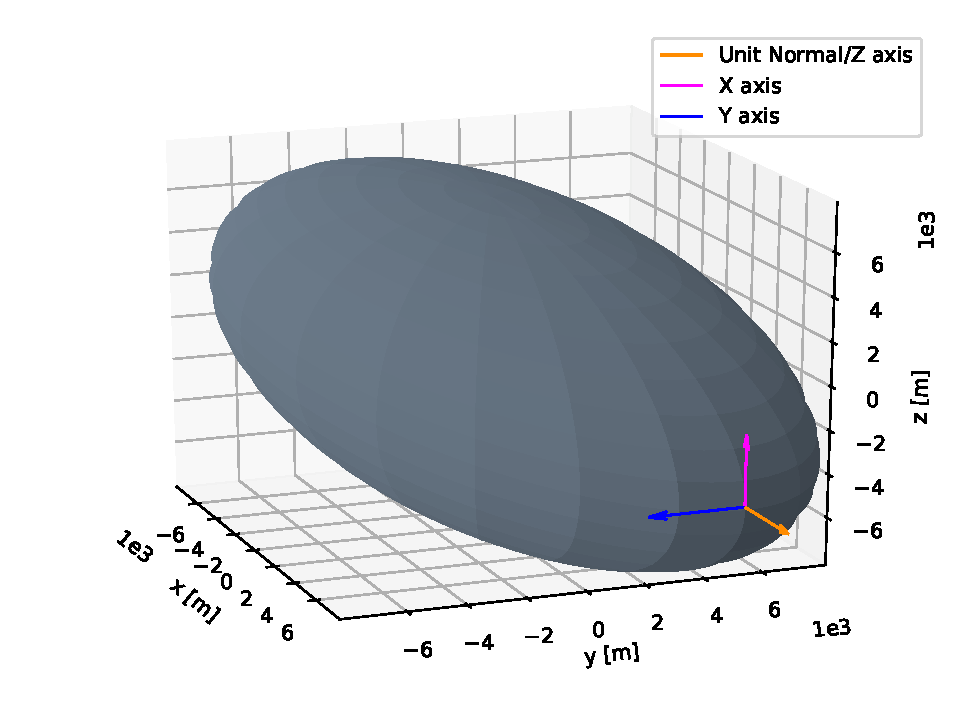
\includegraphics[width=\textwidth, height=0.4\textheight, keepaspectratio=true]{surfaceFrame_longestEdge.pdf}
\caption{An example of the \gls{SF} at the launch location of latitude and longitude \SI{0}{\degree} i.e. the longest edge of the asteroid. The x-axis points to the local North; z-axis is in the direction of the unit normal vector at the launch location; and finally the y-axis completes right-hand rule orthogonal frame.}
\label{fig:surface_frame}
\end{figure}
\FloatBarrier
%%%
As said earlier, the x-basis vector for the \gls{SF} can not be defined by the method described previously for launch locations on the two poles of the asteroid. Hence we use two alternate definitions for the x-basis vector in those scenarios however all other computations remain the same as described before. If the launch location is the North pole, then the x-basis vector of the \gls{SF} is defined as $\buv{x}=[1, 0, 0]$ and for South pole it is defined as $\buv{x}=[-1, 0, 0]$.

\section{Non-conservative Guarantee Escape Speed}
\label{sec:escape_speed_derivation}
Up until now we discussed the dynamics involved with the particle motion around an asteroid and we also devised methods to launch regolith from the surface into an orbit. It was mentioned earlier that the thesis has employed a full numerical simulation approach to the problem at hand, but while doing that we did attempt at finding a new analytical method to determine a non-conservative guarantee escape speed.
%
\newline\newline
%
The conservative guarantee escape speed method is obtained by making use of the maximum gravity potential, between the actual potential of the irregular body and an equivalent point mass potential, at the location of the launch of the particle. If the launch speed is above the conservative guarantee escape speed, then the particle will escape immediately after launch. The conservative guaranteed escape speed method works best for uniform gravity field models, as we'll see later in \Cref{subsec:nonconservative}, but fails when one accounts for non-uniform gravity field models such as the \gls{CDE} model.
% This method however, does not account for the cases which result in an escape situation after completing one or more orbital revolutions around the asteroid or basically the cases where the launch speed is below the conservative guarantee escape speed and still result in an escape scenario. The idea of developing a new analytical method stems from this problem and we call it the non-conservative guarantee escape speed since we aim to account for those cases as well where the escape does not happen immediately.
%
\newline\newline
%
We will first understand how the conventional guarantee escape speed is obtained since it will help us in understanding the method for the non-conventional guarantee escape speed later on. The inertial velocity of a particle which is resting on an asteroid's surface is given as $\bv{v}_I = \bv{\omega} \times \bv{r}$, where \bvt{r} is the location to the particle from the centre of the asteroid. The resulting vector is pointing outwards from the asteroid if the launch location is on the leading edge of the asteroid and inwards if the launch location is on the trailing edge of the asteroid \parencite{scheeresBook}. The idea is easily depicted in \Cref{fig:conservative_escape_speed_leading_trailing_edges}.
%%%
\begin{figure}[htb]
\centering
\captionsetup{justification=centering}
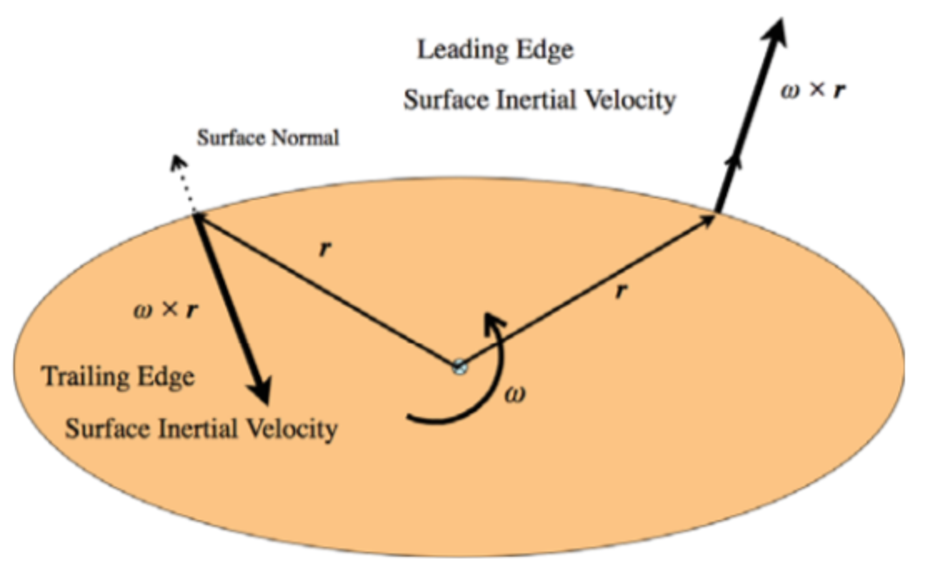
\includegraphics[width=\textwidth, height=0.3\textheight, keepaspectratio=true]{leading_trailing_edge.pdf}
\caption{Schematic for inertial velocity at the surface for different launch locations \parencite{scheeresBook}.}
\label{fig:conservative_escape_speed_leading_trailing_edges}
\end{figure}
\FloatBarrier
%%%
The idea now is to provide an additional launch speed, for instance in the normal direction, that would result in an escape scenario for the particle. The inertial velocity can then be expressed as follows \parencite{scheeresBook}:
%%%
\begin{align}
    \bv{v}_I &= v_{e}\buv{n} + \bv{\omega} \times \bv{r}
    \label{eqn:conservative_inertial_escape}
\end{align}
%%%
where $v_e\buv{n}$ is the velocity, expressed in \gls{ARF}, with which a particle is launched in the normal direction such that the particle is on an escape trajectory. All other terms have been defined previously. The conservative approach is to equate $\bv{v}_I$ to $\sqrt{2U_{max}}$ where $U_{max} = max[U(\bv{r}), \mu/\bv{r}]$ \parencite{scheeresBook}. \Cref{eqn:conservative_inertial_escape} can then be re-written as follows:
%%%
\begin{align}
    \sqrt{2U_{max}} &= v_{e}\buv{n} + \bv{\omega} \times \bv{r} \\
    2U_{max} &= v_e^2 + (\bv{\omega} \times \bv{r})^2 + 2 v_e (\buv{n} \cdotp (\bv{\omega} \times \bv{r}))
    \label{eqn:conservative_quadratic}
\end{align}
%%%
\Cref{eqn:conservative_quadratic} is a quadratic equation in $v_e$ and can be solved as follows:
%%%
\begin{align}
    v_e &= \frac{-2(\buv{n} \cdotp (\bv{\omega} \times \bv{r})) \pm \sqrt{4 (\buv{n} \cdotp (\bv{\omega} \times \bv{r}))^2 + 4 (2U_{max}) - 4(\bv{\omega} \times \bv{r})^2}}{2} \\
    v_e &= -(\buv{n} \cdotp (\bv{\omega} \times \bv{r})) \pm \sqrt{(\buv{n} \cdotp (\bv{\omega} \times \bv{r}))^2 + 2U_{max} - (\bv{\omega} \times {\bv{r}})^2}
\end{align}
%%%
Since the speed can not be negative, the formula is re-written as:
%%%
\begin{align}
    v_e &= -(\buv{n} \cdotp (\bv{\omega} \times \bv{r})) + \sqrt{(\buv{n} \cdotp (\bv{\omega} \times \bv{r}))^2 + 2U_{max} - (\bv{\omega} \times {\bv{r}})^2}
    \label{eqn:conservative_escape_speed}
\end{align}
%%%
\Cref{eqn:conservative_escape_speed} thus gives the conservative escape speed, expressed in the \gls{ARF}, for a particle launched in the normal direction. The equation is equally applicable for a particle launched in any general direction as well by substituting $\buv{n}$ with the unit vector for the direction in which the launch takes place. Thus if a particle is launched with a velocity above or equal to the one mentioned in \Cref{eqn:conservative_escape_speed}, then it would result in a guaranteed escape situation.
%
\newline\newline
%
Now for a non-conservative approach, we will not use $\bv{v}_I = \sqrt{2U_{max}}$ to get a guaranteed escape launch speed. We will derive an alternate relation for $\bv{v}_I$ first and then later on substitute it back into \Cref{eqn:conservative_escape_speed} in place of $2U_{max}$ to get the non-conservative guaranteed escape launch speed.
%
\newline\newline
%
Consider the \gls{EOM} mentioned in \Cref{eqn:p2bp}, with the exception that we only consider the gravity potential and remove all external perturbations on the left hand side of the equation. These equations do not have an explicit dependence on time which means that the Jacobian for the system exists and is conserved \parencite{scheeresBook}. The Jacobian, expressed in the \gls{ARF}, is given as follows \parencite{scheeresBook}:
%%%
\begin{align}
    J &= \frac{1}{2} v_B^2 - \frac{1}{2} \omega^2(x^2 + y^2) - U(\bv{r})
    \label{eqn:jacobian}
\end{align}
%%%
where $v_B$ is the velocity of the particle in the \gls{ARF}; $\omega$ is the magnitude of the angular velocity of the rotating asteroid and is along the z-axis of the \gls{ARF}; $(x,y)$ are the x-y coordinate of the orbiting particle; $U(\bv{r})$ is the small-body gravity potential, which in our case is the \gls{CDE} potential model. From transport theorem, we use the relation between an inertial velocity and the rotating frame velocity:
%%%
\begin{align}
    \bv{v}_B &= \bv{v}_I - (\bv{\omega} \times \bv{r}) \\
    v_B^2 &= v_I^2 + (\bv{\omega} \times \bv{r})^2 - 2 \bv{v}_I \cdotp (\bv{\omega} \times \bv{r}) \\
    v_B^2 &= v_I^2 + (\bv{\omega} \times \bv{r})^2 - 2 \bv{\omega} \cdotp (\bv{r} \times \bv{v}_I) \\
    v_B^2 &= v_I^2 + (\bv{\omega} \times \bv{r})^2 - 2 \bv{\omega} \cdotp \bv{H}
    \label{eqn:arf_velocity_modified_with_H}
\end{align}
%%%
where \bvt{H} is the angular momentum of the orbiting particle. We substitute \Cref{eqn:arf_velocity_modified_with_H} back into \Cref{eqn:jacobian} to get the following relation:
%%%
\begin{align}
    J &= \frac{1}{2} v_I^2 - \bv{\omega} \cdotp \bv{H} - U(\bv{r})
    \label{eqn:jacobian_mod}
\end{align}
%%%
Considering that after launch the particle is on a parabolic trajectory such that it barely escapes then in such a case the energy of the particle would be 0 which reduces the Jacobian to $J_{\infty} = -\bv{\omega} \cdotp \bv{H}_{\infty}$. Now at the instance of the launch, the Jacobian is expressed as follows:
%%%
\begin{align}
    J_0 &= \frac{1}{2} v_{I_0}^2 - \bv{\omega} \cdotp \bv{H}_0 - U(\bv{r}_0)
    \label{eqn:jacobian_t0}
\end{align}
%%%
Since the Jacobian is conserved, $J_0 = J_{\infty}$, which means we can write the following relation:
%%%
\begin{align}
    \frac{1}{2} v_{I_0}^2 - \bv{\omega} \cdotp \bv{H}_0 - U(\bv{r}_0) &= -\bv{\omega} \cdotp \bv{H}_{\infty}
    \label{eqn:jacobian_equate}
\end{align}
%%%
For parabolic trajectories, the angular momentum magnitude is expressed in terms of the semi-latus rectum and the gravitational parameter of the central body as $H = \sqrt{\mu 2q}$ where $q$ is the periapsis distance \parencite{schaub2003Book}. Also the angle between the angular momentum vector and the asteroid's rotation vector is the orbit inclination ($i$) and with these new definitions, \Cref{eqn:jacobian_equate} is re-written as follows:
%%%
\begin{align}
    \frac{1}{2} v_{I_0}^2 - \bv{\omega} \cdotp \bv{H}_0 - U(\bv{r}_0) &= -\omega \cos(i) \sqrt{2\mu q_{\infty}}
    \label{eqn:jacobian_equate_cosi}
\end{align}
%%%
We will consider only equatorial orbits for now and hence \Cref{eqn:jacobian_equate_cosi} can be stated as simply:
%%%
\begin{align}
    \frac{1}{2} v_{I_0}^2 - \bv{\omega} \cdotp \bv{H}_0 - U(\bv{r}_0) &= -\omega \sqrt{2\mu q_{\infty}} \\
    \frac{1}{2} v_{I_0}^2 - \bv{\omega} \cdotp (\bv{r}_0 \times \bv{v}_{I_0}) - U(\bv{r}_0) &= -\omega \sqrt{2\mu q_{\infty}}
    \label{eqn:jacobian_equate_equatorial}
\end{align}
%%%
Note we can write $H_0 = \bv{r}_0 \times \bv{v}_{I_0}$, where $\bv{r_0}$ is expressed in \gls{ARF}, since at time $t = 0$ both \gls{ARF} and \gls{AIF} are aligned which means that $\bv{r}_{I_0} = \bv{r}_{B_0}$. The intent now is to solve for $v_{I_0}$ from \Cref{eqn:jacobian_equate_equatorial}, which is the inertial velocity at launch that eventually leads to an escape scenario.
%%%
\begin{figure}[htb]
\centering
\captionsetup{justification=centering}
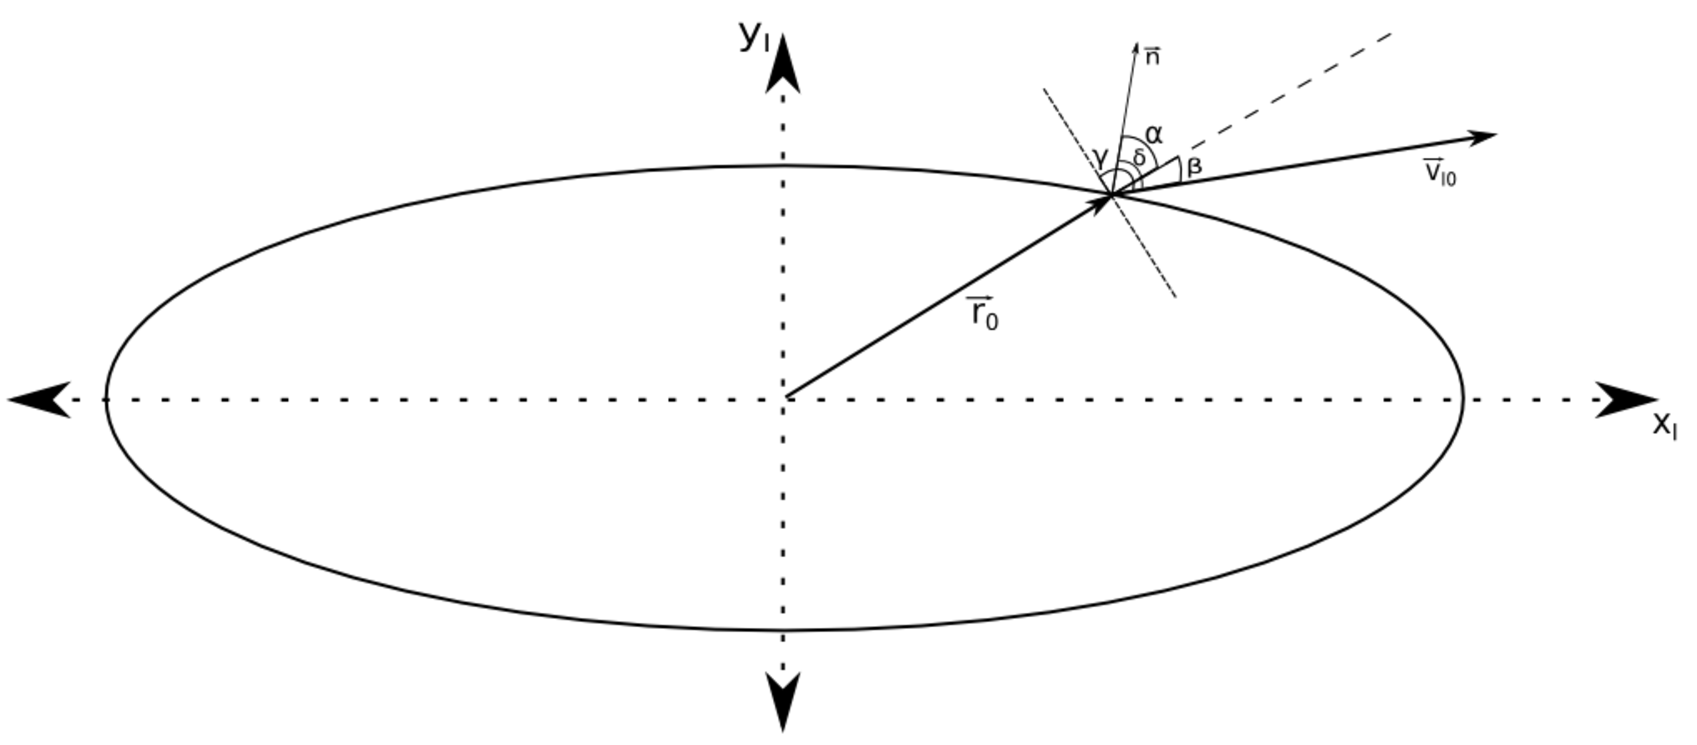
\includegraphics[width=\textwidth, height=0.3\textheight, keepaspectratio=true]{non_conservative_escape_velocity_angles.pdf}
\caption{General angle definitions for velocity vector with position and normal vector at the launch location.}
\label{fig:velocity_vector_angles}
\end{figure}
\FloatBarrier
%%%
We need to evaluate the second term on the left hand side of \Cref{eqn:jacobian_equate_equatorial} using the angle definitions given in \Cref{fig:velocity_vector_angles}. In that, $\gamma$ is the angle between the velocity vector and the plane perpendicular to the position vector; $\delta$ is the launch declination angle as explained in \Cref{subsec:launch_velocity}; $\alpha$ is the angle between the normal vector and the position vector direction and finally, $\beta$ is the angle between the velocity vector and the position vector direction. Using these definitions, the cross product in \Cref{eqn:jacobian_equate_equatorial} is evaluated as follows:
%%%
\begin{align}
    \bv{\omega} \cdotp (\bv{r}_0 \times \bv{v}_{I_0}) &= \bv{\omega} \cdotp (r_0 v_{I_0} \sin(\beta) \buv{h}) \\
    % &= \omega r_0 v_{I_0} \sin(-(90 - \gamma)) \\
    % &= -\omega r_0 v_{I_0} \cos(\gamma) \\
    % &= -\omega r_0 v_{I_0} \cos(90 - \alpha + \delta) \\
    % &= -\omega r_0 v_{I_0} \sin(\alpha - \delta) \\
    &= (r_0 v_{I_0} \sin(\delta - \alpha)) \bv{\omega} \cdotp \buv{h}
    \label{eqn:cross_product_eval}
\end{align}
%%%
where $\buv{h}$ specifies the direction of the cross product, i.e. the angular momentum vector $\bv{H}_0$. The angle definitions given in \Cref{fig:velocity_vector_angles} remains valid even for a launch location at the trailing edge of the asteroid and hence the angular definitions remain generalized. In addition to having an equatorial orbit, we can further simplify \Cref{eqn:cross_product_eval} by keeping the launch site at the longest edge of the ellipsoid which means that we can make $\alpha=0$. Thus \Cref{eqn:jacobian_equate_equatorial} can be re-written as:
%%%
\begin{align}
    \frac{1}{2} v_{I_0}^2 - (r_0 v_{I_0} \sin(\delta)) \bv{\omega}\cdotp\buv{h} - U(\bv{r}_0) &= -\omega \sqrt{2\mu q_{\infty}}
    \label{eqn:jacobian_equate_equatorial_mod}
\end{align}
%%%
\Cref{eqn:jacobian_equate_equatorial_mod} is a quadratic equation in $v_{I_0}$ which is solved to provide the following solution:
%%%
\begin{align}
    v_{I_0} &= (r_0 \sin\delta) \bv{\omega}\cdotp\buv{h} \pm \sqrt{((r_0 \sin\delta)\bv{\omega}\cdotp\buv{h})^2 + 2U - 2\omega\sqrt{2\mu q_\infty}}
    \label{eqn:non_conservative_inertial_guaranteed_escape_speed}
\end{align}
%%%
Thus instead of using $v_{I_0} = \sqrt{2U_{max}}$ in \Cref{eqn:conservative_quadratic}, we use the formula in \Cref{eqn:non_conservative_inertial_guaranteed_escape_speed} which leads to modifying \Cref{eqn:conservative_escape_speed} as follows:
%%%
\begin{align}
    v_e &= -(\buv{d} \cdotp (\bv{\omega} \times \bv{r})) + \sqrt{(\buv{d} \cdotp (\bv{\omega} \times \bv{r}))^2 + v_{I_0}^2 - (\bv{\omega} \times {\bv{r}})^2}
    \label{eqn:nonconservative_escape_speed}
\end{align}
%%%
where instead of using $\buv{n}$ we use the unit vector $\buv{d}$, representing a general direction of launch and not just the normal direction. Note that \Cref{eqn:jacobian_equate_equatorial_mod,eqn:non_conservative_inertial_guaranteed_escape_speed} are valid only for the launch location at the longest edge of the ellipsoid. We simplified the equations by making $\alpha=0$ so that testing this approach for a non-conservative guaranteed escape speed can be made easy, however the approach can be generalized by using a non-zero value for $\alpha$ in \Cref{eqn:cross_product_eval} as well.

% \section{Conclusion}
% \label{sec:dynamics_conclusion}

% \chapter{NAOS: Near-Asteroid Orbit Simulator}
\label{chap:naos}
\graphicspath{{NAOS/Images/}}

% \chapter{Verification \& Validation}
\label{chap:v_and_v}
\graphicspath{{V&V/Images/}}

\part{Numerical Simulation Results}
\chapter{Guaranteed Escape Speed}
\label{chap:nonconservative}
\graphicspath{{Results/Images/}}

In this chapter, we will discuss the results from the non-conservative guaranteed escape speed analytical method developed in \Cref{sec:escape_speed_derivation}. The algorithm's absolute performance and its viability is discussed and compared with that of the conservative guaranteed escape speed algorithm.

\section{Simulation Setup}
\label{sec:nonconservative_simulation_setup}
As mentioned in \Cref{sec:escape_speed_derivation}, the launch location for testing out the algorithm was chosen to be the longest edge of the ellipsoid shaped asteroid since it helped in simplifying the computation. In addition to this, the particles were launched in the equatorial plane such that the orbital inclination remained zero \footnote{The orbital inclination remains zero valued after the launch in a non-uniform gravity field because the central body is homogeneous as well as symmetrical about the equator which means that there is equal attraction in the positive and negative z-axis directions which cancel each other out.}, which further simplified the computation.
%
\newline\newline
%
We compare the results from our derivation of the non-conservative guaranteed escape speed with that of the conservative approach as defined by \cite{scheeresBook}. To use the algorithm, the following launch conditions were used (these launch conditions are also depicted in \Cref{fig:non_conservative_launch_vectors}):
%%%
\begin{enumerate}
    \item The launch location is at the longest edge of the ellipsoid.
    \item The launch azimuth is equal to \SI{270}{\degree}.
    \item The launch declinations are varied from \SI{10}{\degree} to \SI{80}{\degree}.
    \item The launch velocity was kept fixed and chosen at random to be \SI{6.0}{\metre \per \second}
\end{enumerate}
%%%
Note that these launch conditions result in equatorial orbits, just like how we want to test the non-conservative escape speed algorithm. The value for the parameter $q_\infty$ in \Cref{eqn:non_conservative_inertial_guaranteed_escape_speed}, which is the periapsis distance for a parabolic escape trajectory, was set manually for each simulated trajectory and remained constant during the entire duration of each simulation. Several values of $q_\infty$ were used for testing and they were all taken as fractions of the largest dimension of the ellipsoid. This was done because we do not yet have a dedicated process to determine the value of $q_\infty$ and hence several random fractions were used to guage the output.
% Note that $q_\infty$ is the distance from the focus to the vertex of a parabola so in this case it is the distance between the centre of the asteroid and the periapsis distance on the final parabolic escape trajectory. We say \emph{final} because the non-conservative guaranteed escape speed was designed to account for regolith cases that do not immediately lead to an escape scenario after being lofted from the surface of an asteroid but rather take one or more orbital revolutions around the asteroid before embarking on the parabolic escape trajectory. We will witness such a case shortly.
%%%
\begin{figure}[htb]
\centering
\captionsetup{justification=centering}
\subfloat[]{
    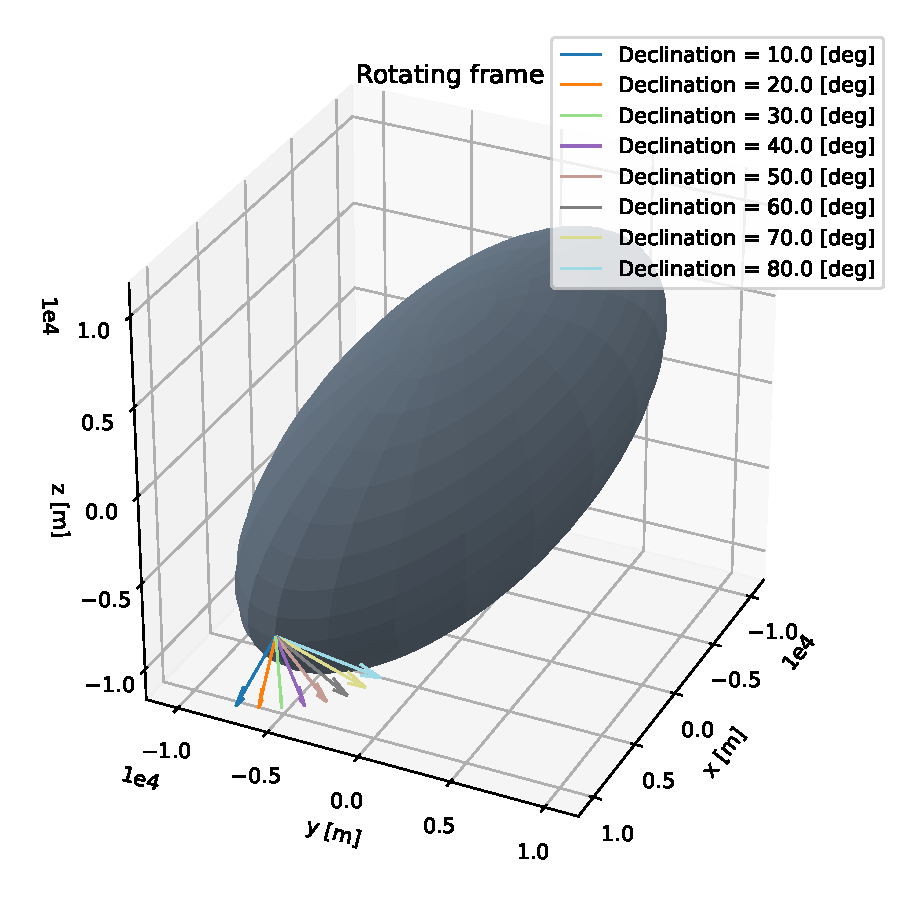
\includegraphics[width=\textwidth, height=0.5\textheight, keepaspectratio=true]{non_conservative_escape_speed/launch_vectors_body_frame.pdf}
    \label{fig:non_conservative_launch_vectors_arf}
}

\subfloat[]{
    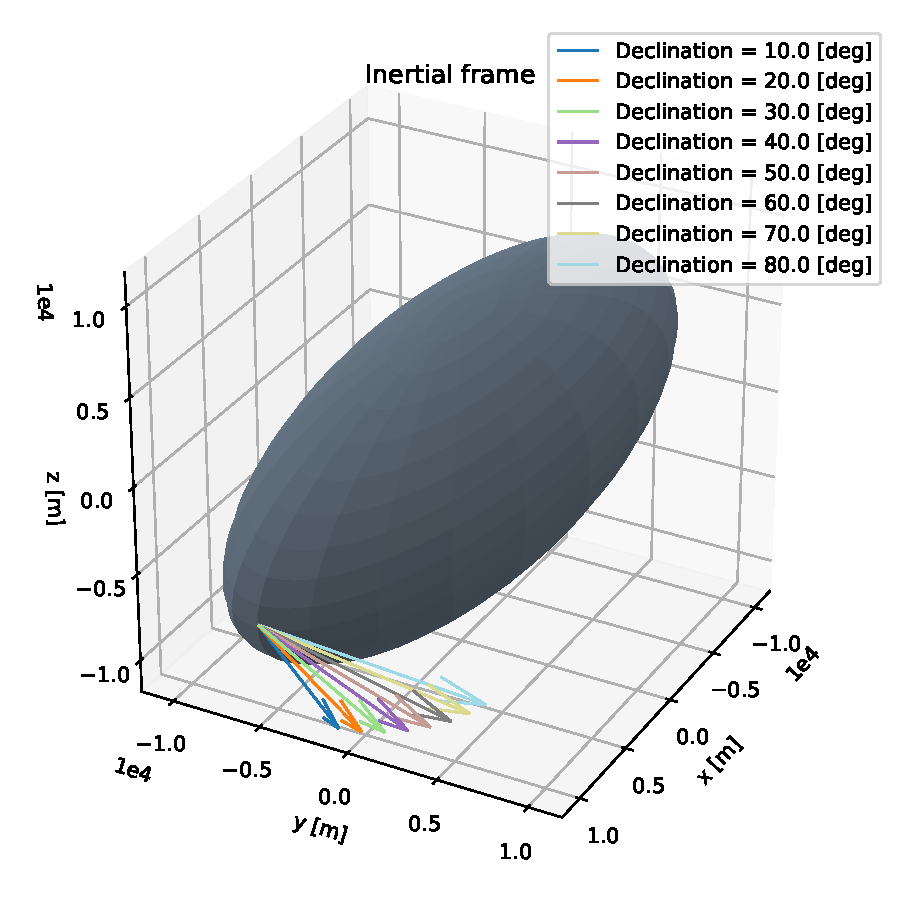
\includegraphics[width=\textwidth, height=0.5\textheight, keepaspectratio=true]{non_conservative_escape_speed/launch_vectors_inertial_frame.pdf}
    \label{fig:non_conservative_launch_vectors_aif}
}
\caption{Launch vectors used for testing the non-conservative escape speed algorithm. \protect\Cref{fig:non_conservative_launch_vectors_arf} shows the vectors expressed in \gls{ARF} and \protect\Cref{fig:non_conservative_launch_vectors_aif} shows the vectors expressed in \gls{AIF}.}
\label{fig:non_conservative_launch_vectors}
\end{figure}
\FloatBarrier
%%%

\section{Conservative Approach With Spherical Asteroid}
\label{sec:conservative_spherical_asteroid_results}
We will first look at the case of a homogeneous spherical asteroid whose radius is equal to the largest semi-major axis of the \gls{CDE} i.e. \SI{20}{\kilo\metre}. The simulation involved launching particles at a constant declination of \SI{45}{\degree} and for launch azimuth varying in the range [0, 360)\si{\degree}. The launch velocities ranged from 1 - \SI{20}{\metre \per \second} and the simulations did not include perturbations, gravity or otherwise. We used the \gls{CDE} potential model but all three semi-major axes were made equal to \SI{20}{\kilo\metre}. In such a case, the \gls{CDE} gravity potential model acts like a point mass potential model. This situation works for us since the latter is the actual gravity potential model for a point external to a homogeneous spherical body \parencite{macmillanPotential}.
%%%
\begin{figure}[htb]
\centering
\captionsetup{justification=centering}
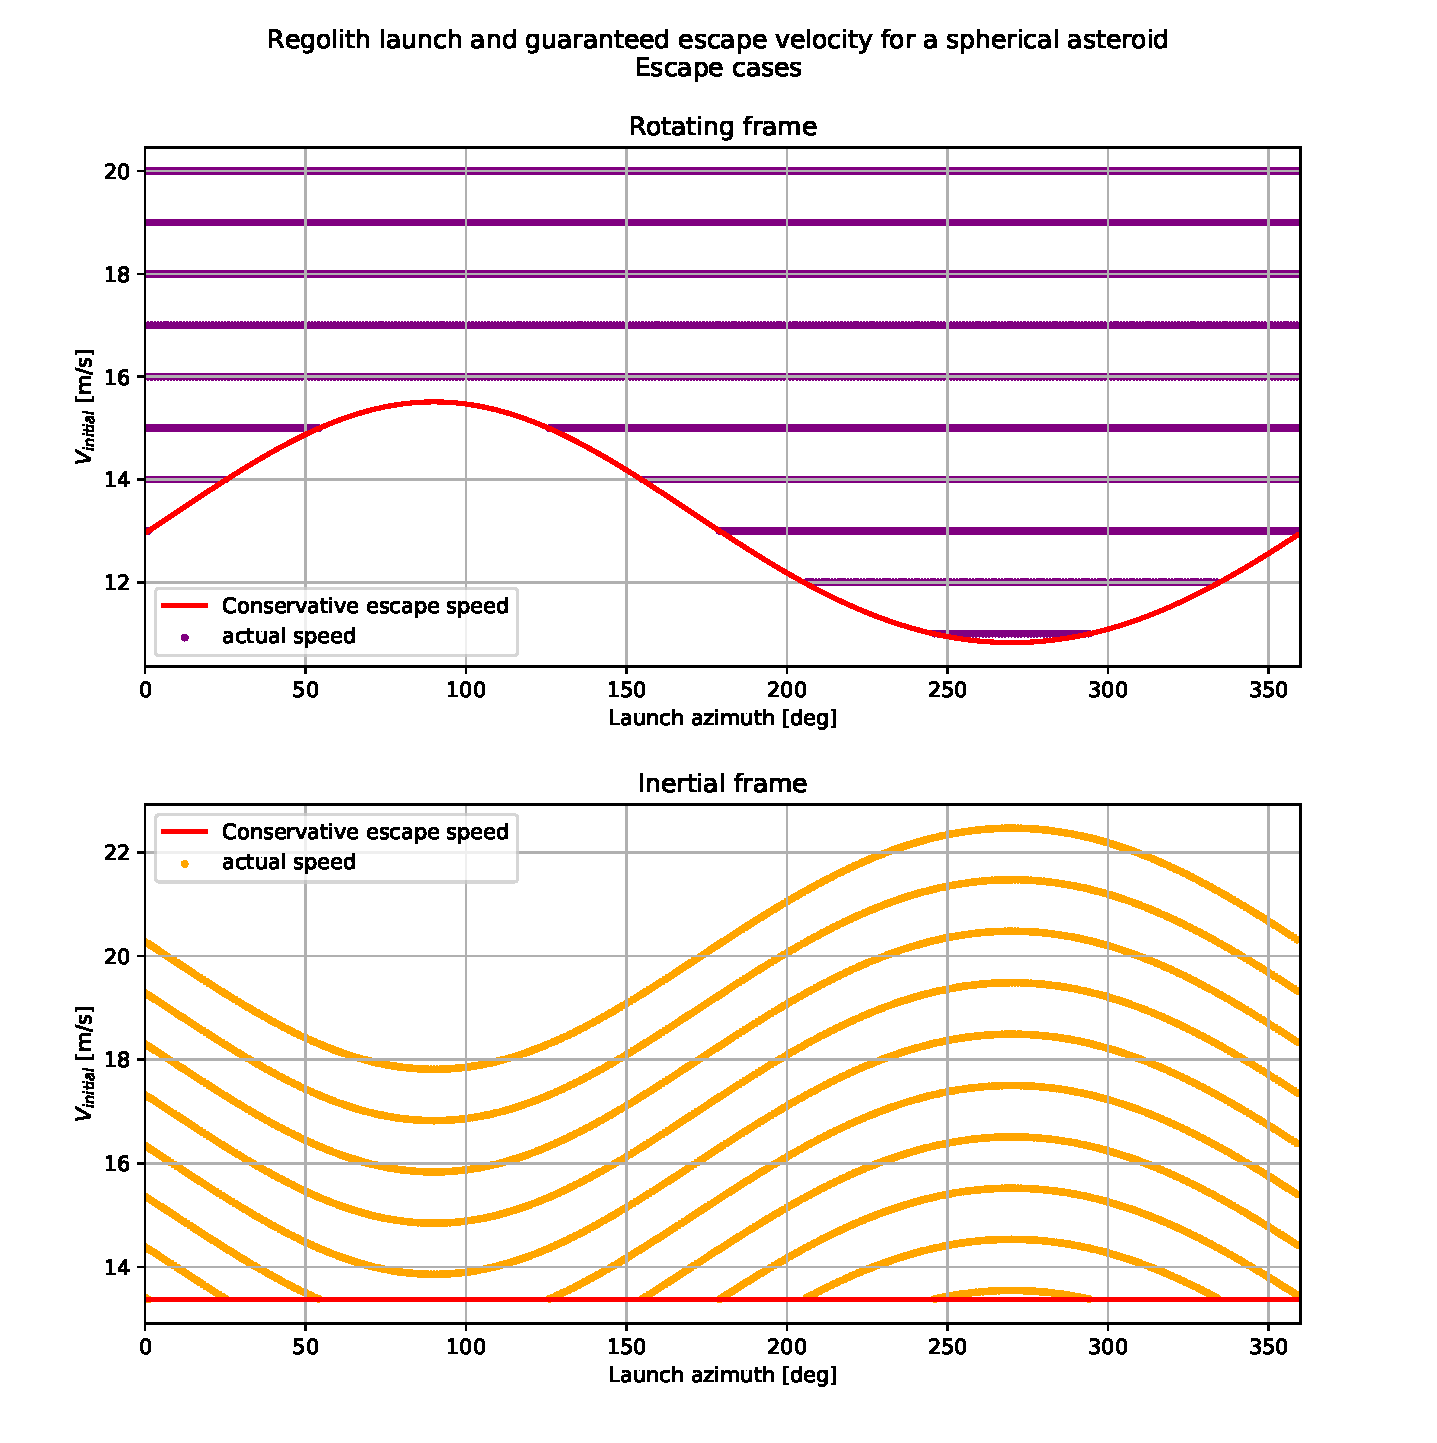
\includegraphics[width=\textwidth, height=0.7\textheight, keepaspectratio=true]{non_conservative_escape_speed/spherical_asteroid_conservative_escape_speed.pdf}
\caption{Escape velocities for varying launch azimuths and a constant launch declination of \protect\SI{45}{\degree}. The conservative guaranteed escape speed curve clearly separates all escape scenarios, as shown in both \protect\gls{AIF} and \protect\gls{ARF}.}
\label{fig:conservative_spherical_asteroid_escape}
\end{figure}
\FloatBarrier
%%%
The algorithm for the conservative guaranteed escape speed works properly for the case of a homogeneous spherical asteroid, as shown in \Cref{fig:conservative_spherical_asteroid_escape}, whose gravity potential is equivalent to that of a point mass. An escape occurs only if the particle was launched with a velocity which is equal to or above the conservative guaranteed escape speed curve and not otherwise. \Cref{fig:conservative_spherical_asteroid_escape_and_reimpact} shows how the curve even separates out all the re-impact cases. All launch velocities that are below the escape speed curve result only in re-impact and nothing else. Note that for this particular simulation we did not obtain any capture cases, but only escape and re-impact.
%%%
\begin{figure}[htb]
\centering
\captionsetup{justification=centering}
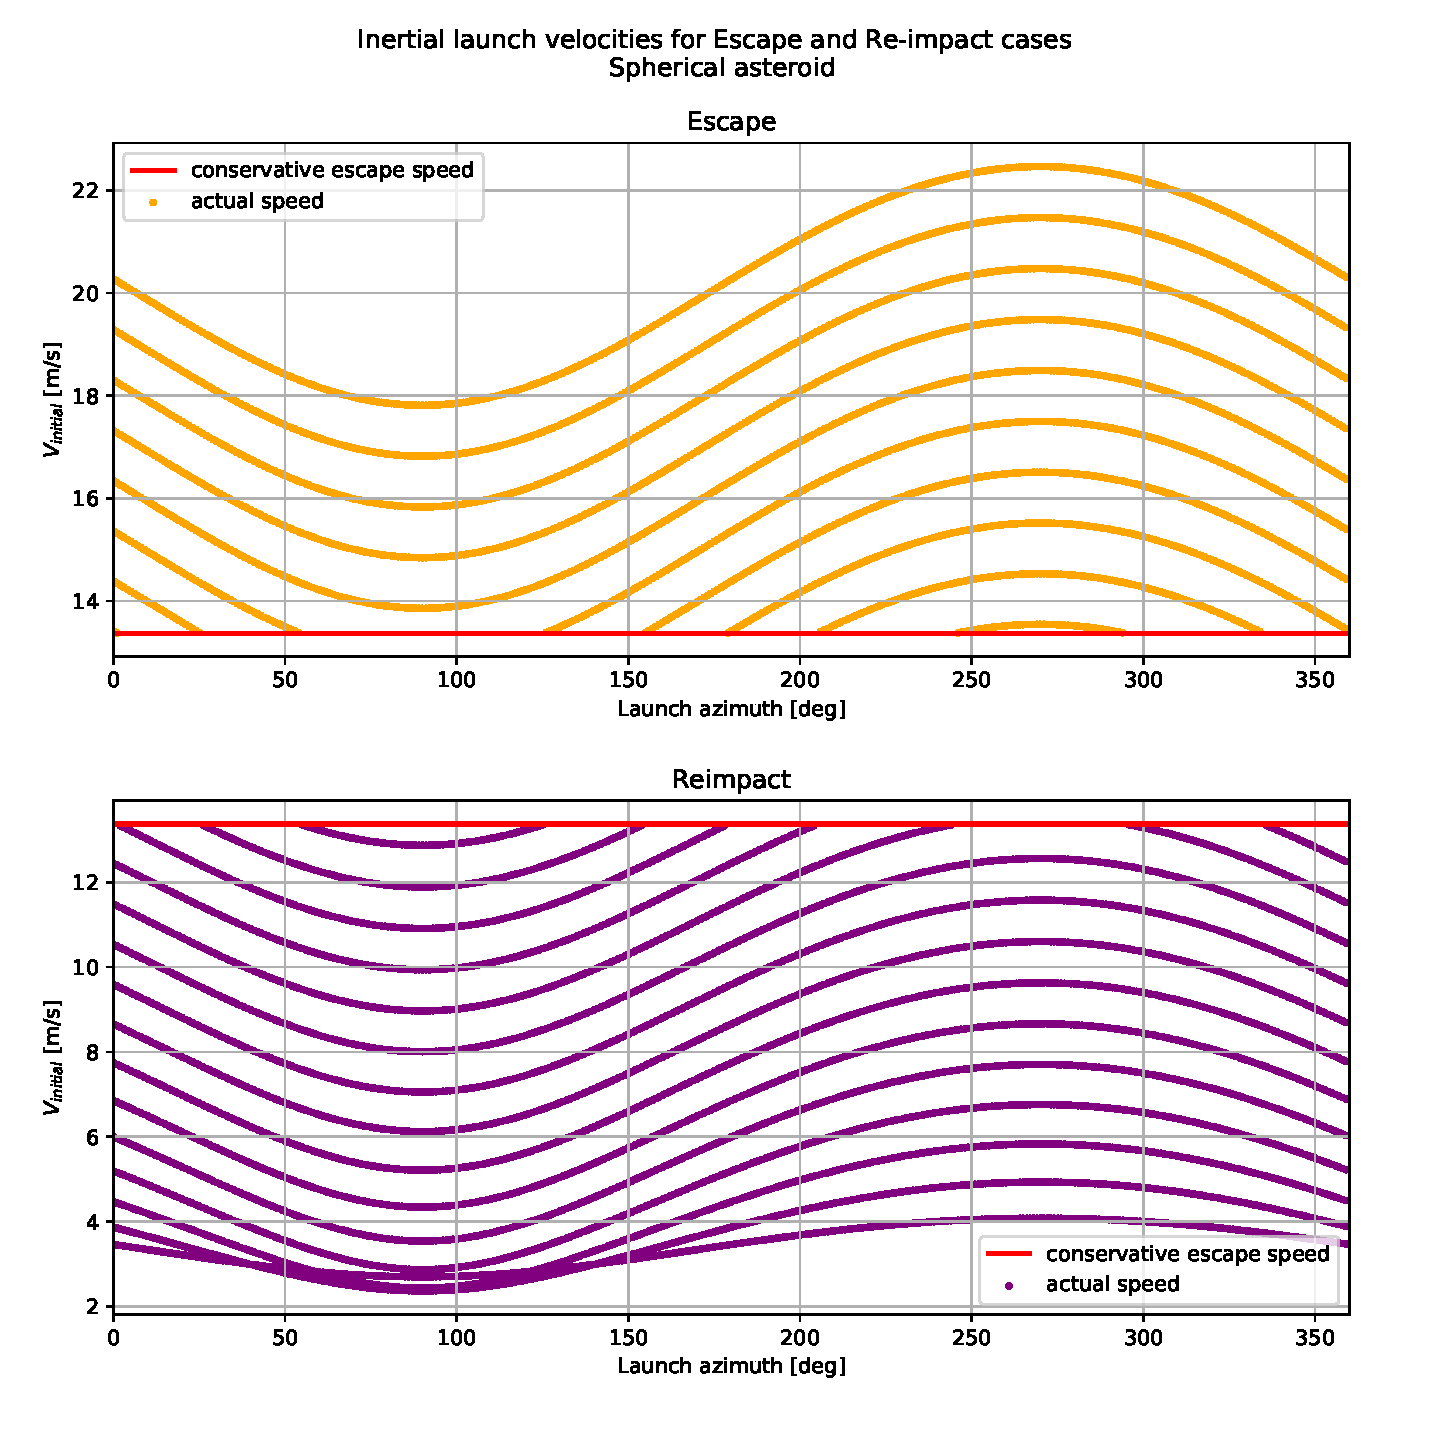
\includegraphics[width=\textwidth, height=0.7\textheight, keepaspectratio=true]{non_conservative_escape_speed/spherical_asteroid_escape_and_capture.pdf}
\caption{Escape and re-impact scenario velocities for varying launch azimuths and a constant launch declination of \protect\SI{45}{\degree}. The conservative guaranteed escape speed curve clearly separates all re-impact cases from the escape ones.}
\label{fig:conservative_spherical_asteroid_escape_and_reimpact}
\end{figure}
\FloatBarrier
%%%

\section{Non-Conservative Approach With Ellipsoidal Asteroid}
\label{sec:nonconservative_escape_cde_results}
Now we shall look at the results for a \gls{CDE} model, for which a particle was launched with the initial conditions enlisted earlier. \Cref{fig:non_conservative_escape_multiple_qinfinity_single_velocity} shows the inadequacy of the conservative guaranteed escape speed algorithm to predetermine escape scenarios based just on the initial conditions, as it fails to account for escape situations that occur at lower declination angles. However, for all launch velocities above the conservative escape speed curve, we only witness escape scenarios which is how it should be and any result contrary to this means the simulator is at fault. The non-conservative escape speed algorithm, does not function as expected. The algorithm was designed, hoping that it would also account for escape cases that the conservative approach was unable to. \Cref{fig:non_conservative_escape_multiple_qinfinity_single_velocity} shows the non-conservative escape speed curves for three different $q_\infty$ values and although we get an idea on the performance from individual $q_\infty$ values, the algorithm in general fails to identify escape scenarios since there are cases (at higher declination angles) where the launch velocity lies below the $q_\infty$ curves but belongs to the escape regime.
%%%
\begin{figure}[htb]
\centering
\captionsetup{justification=centering}
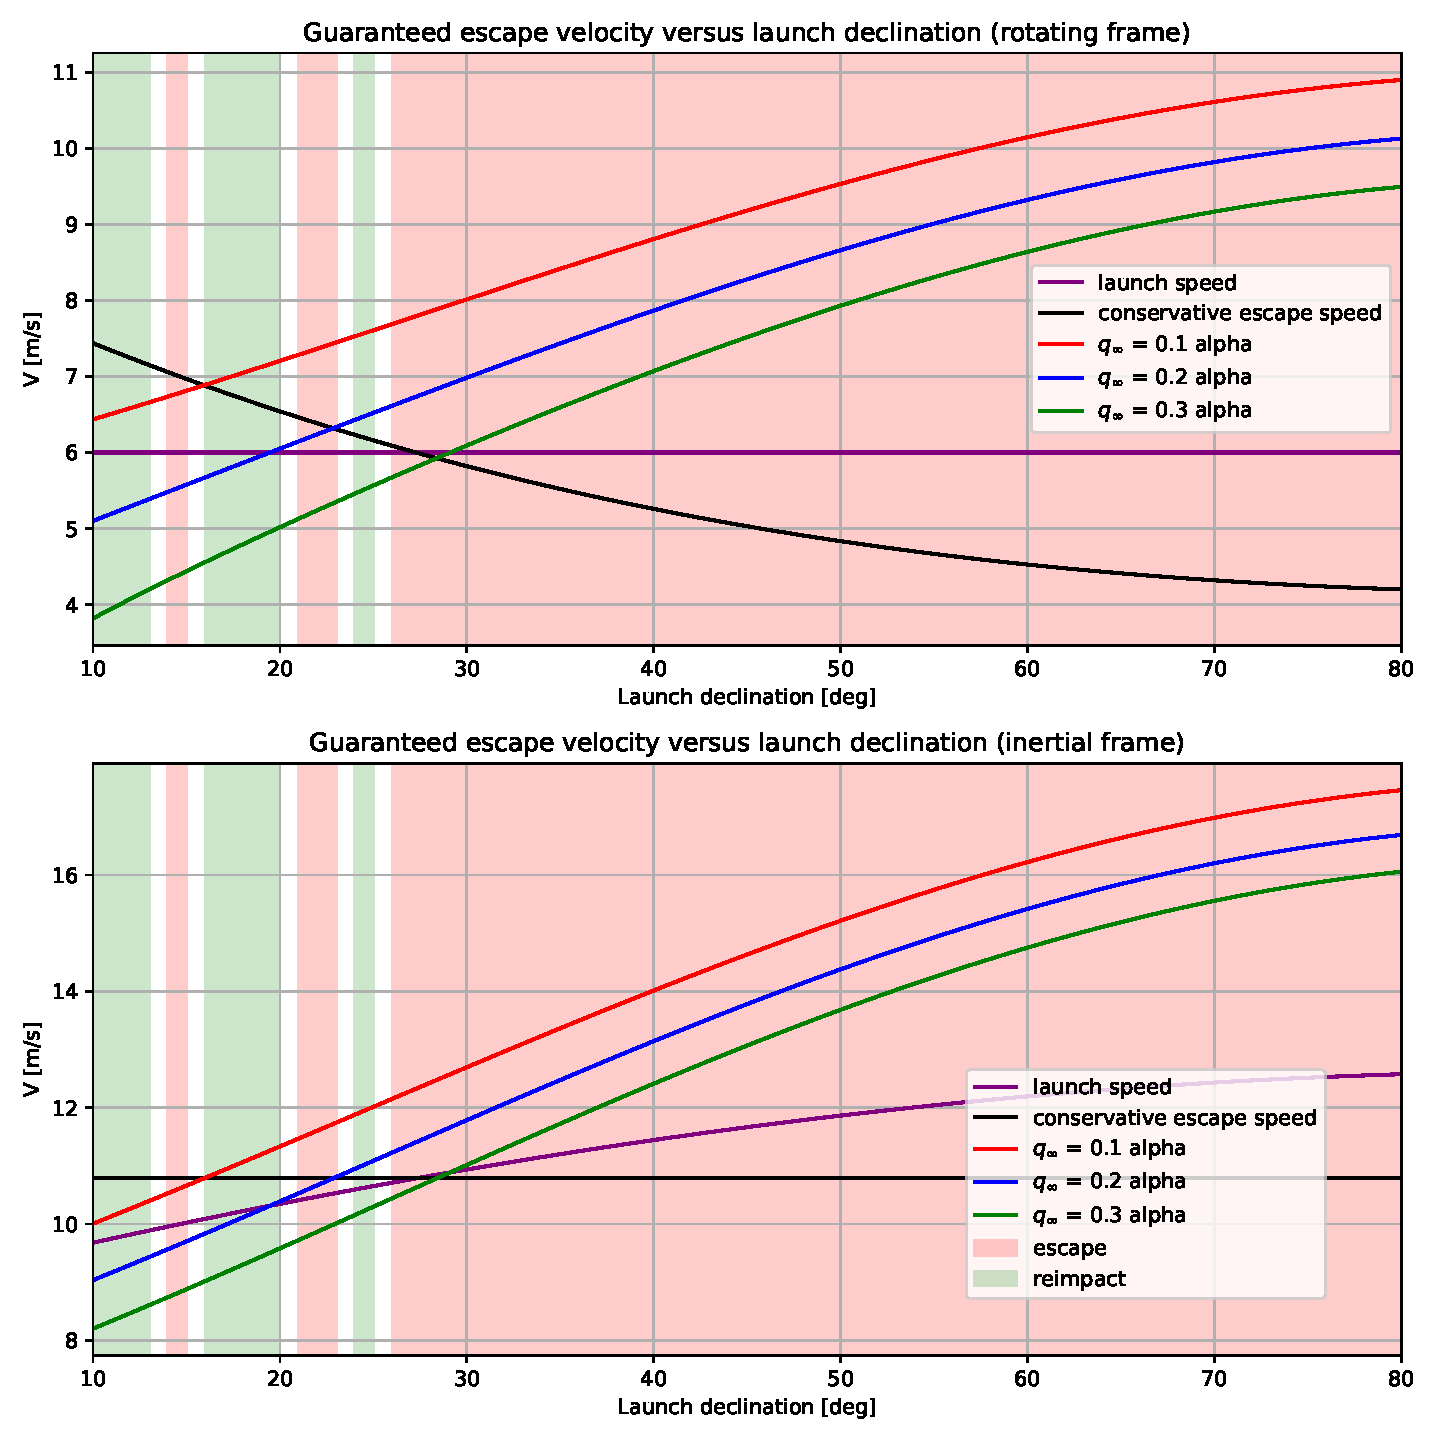
\includegraphics[width=\textwidth, height=0.7\textheight, keepaspectratio=true]{non_conservative_escape_speed/multiple_qinfinity_plus.pdf}
\caption{Escape and re-impact scenarios depicted for regolith launched with a single velocity and launch azimuth but multiple launch declination values. Non-conservative escape speed curve is shown for a \gls{CDE} asteroid for three $q_\infty$ values that are fractions of the largest semi-major axes, $\alpha$, of the ellipsoid. The conservative guaranteed escape speed curve is also shown for comparison.}
\label{fig:non_conservative_escape_multiple_qinfinity_single_velocity}
\end{figure}
\FloatBarrier
%%%
It is important to note that in \Cref{fig:non_conservative_escape_multiple_qinfinity_single_velocity}, the non-conservative escape speed curves used only the \emph{"+"} sign part of the formula in \Cref{eqn:non_conservative_inertial_guaranteed_escape_speed} and not the \emph{"-"} sign part since the latter always gave negative velocities for multiple sample values of $q_\infty$. We performed the simulation for the non-conservative approach for the same launch azimuth and range of declination angles as before but velocities ranging from 1 to \SI{16}{\metre \per \second} and $q_\infty=0.3$ to see if the curve provides better escape estimates at other launch velocities. The result of this is shown in \Cref{fig:non_conservative_multiple_velocities_qinfinity_0.3}. We see yet again the failure of the so called non-conservative escape speed algorithm. We witness that even when the launch velocity is above the non-conservative escape speed curve, we have re-impact scenarios. This clearly means that the algorithm is not even able to demarcate re-impact situations. Atleast with the conservative escape speed curve, we know that if the launch velocity is above the curve then the regolith can only escape and not have any other final fate.
%%%
\begin{figure}[htb]
\centering
\captionsetup{justification=centering}
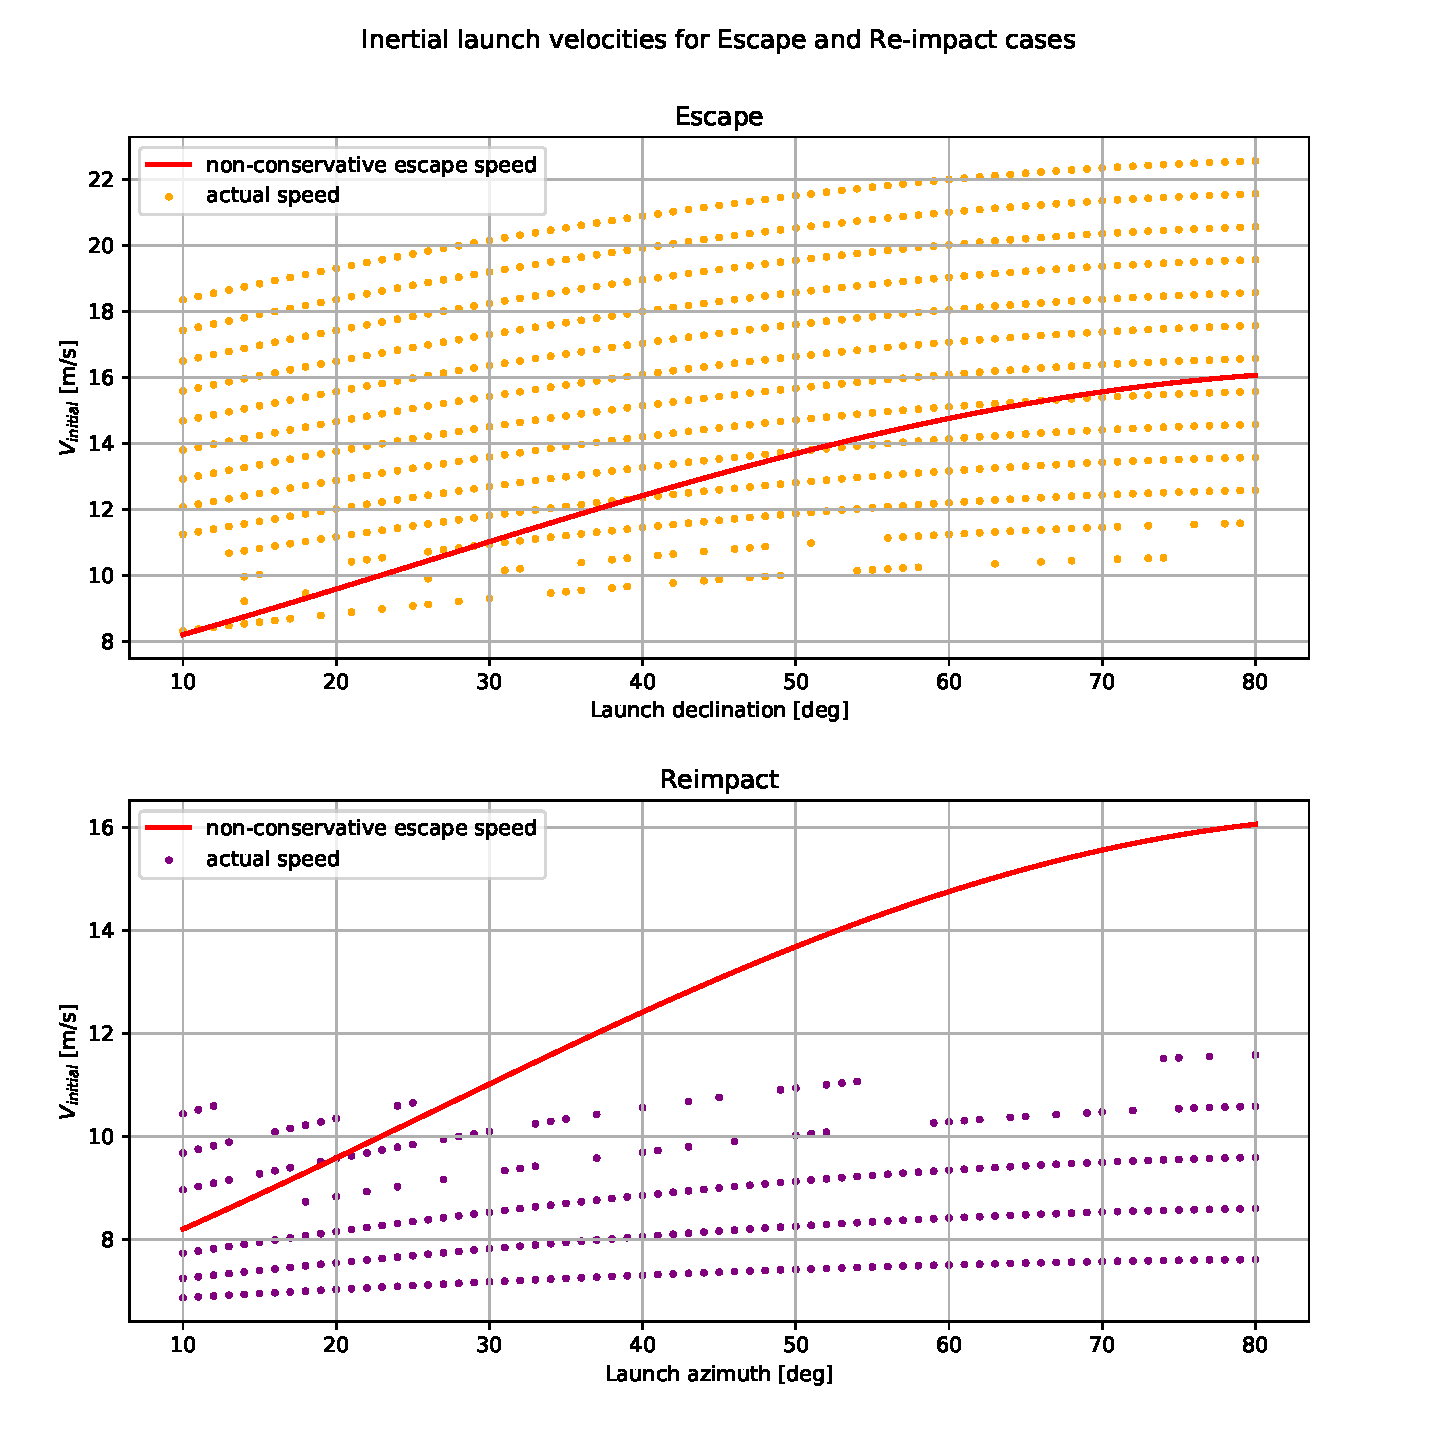
\includegraphics[width=\textwidth, height=0.7\textheight, keepaspectratio=true]{non_conservative_escape_speed/qinfinity_dot3_escape_reimpact_multipleVelocities.pdf}
\caption{Escape and re-impact scenarios depicted for regolith launched from the longest edge of \gls{CDE} with multiple velocities with launch azimuth = \SI{270}{\degree} and launch declination in the range of 10 to \SI{80}{\degree}. The non-conservative escape speed curve is shown for $q_\infty = 0.3$.}
\label{fig:non_conservative_multiple_velocities_qinfinity_0.3}
\end{figure}
\FloatBarrier
%%%
On the other end of the spectrum, we can see that there are launch velocities below the non-conservative escape speed curve where escape scenarios occur. This is another indication of the failure of the algorithm we designed.
%
\newline\newline
%
The other problem with the algorithm is that if we reduce the value of $q_\infty$ beyond certain extent, then we obtain a gibberish curve for the non-conservative escape speed in the \gls{ARF}. An example of this is depicted in \Cref{fig:non_conservative_qinfinity_0.7} where $q_\infty = 0.7$. The curve as expressed in the \gls{ARF} has no meaning since negative speeds are not valid.
%%%
\begin{figure}[htb]
\centering
\captionsetup{justification=centering}
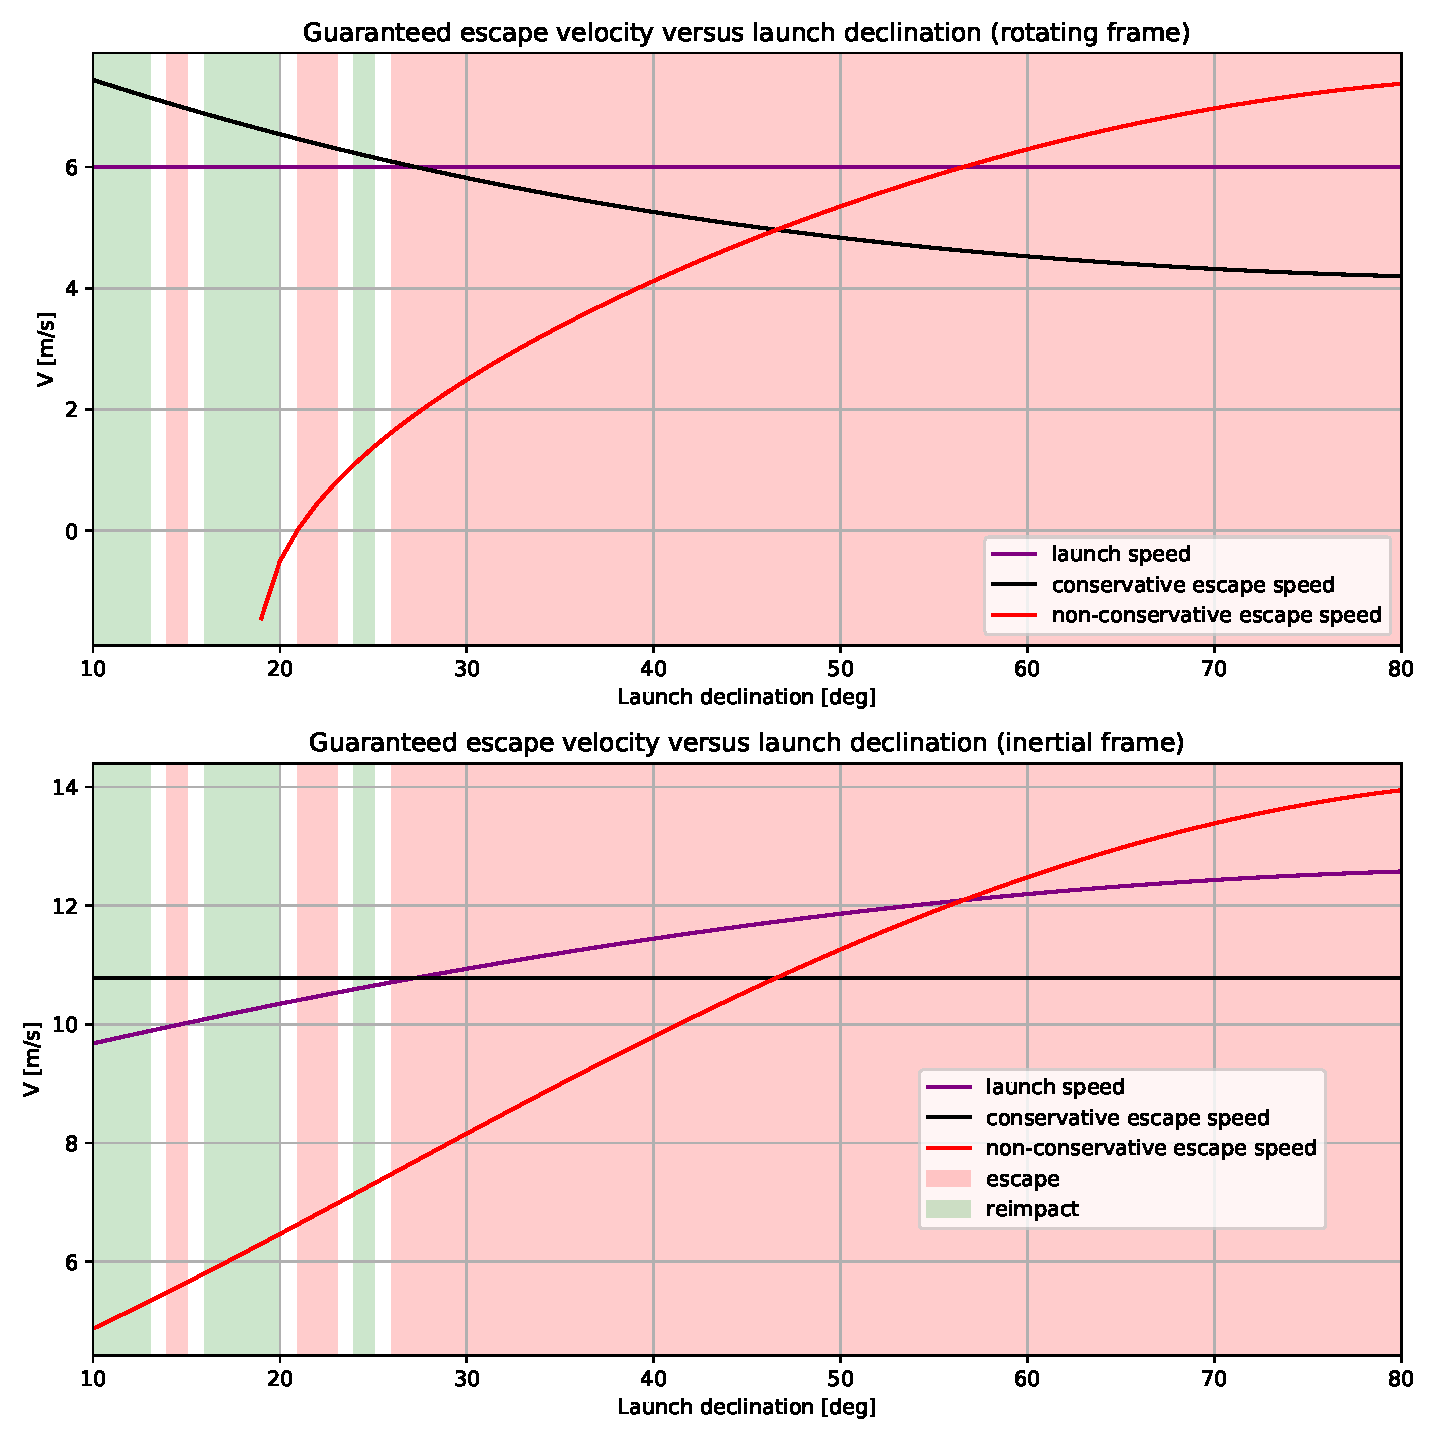
\includegraphics[width=\textwidth, height=0.6\textheight, keepaspectratio=true]{non_conservative_escape_speed/qinfinity_dot7alpha_plus.pdf}
\caption{A non-applicable non-conservative escape speed curve for $q_\infty=0.7$. The curve in the rotating frame or the \gls{ARF} shows negative speed values which is not valid.}
\label{fig:non_conservative_qinfinity_0.7}
\end{figure}
\FloatBarrier
%%%
The non-conservative guaranteed escape speed method did not work as expected in identifying the escape cases that were undetected by the conservative method. In addition to this, we saw that the method produces a valid escape velocity curve only for a small range of $q_\infty$ values. Although the non-conservative method failed, the approach to derive it was correct and now we know that even if it sounds reasonable in theory, it fails completely in practice.

\section{Conservative Approach Limitations With Ellipsoidal Asteroid}
\label{sec:conservative_escape_cde_limitations}
The conservative escape speed approach didn't account for a few escape scenarios when regolith was launched from the surface of a \gls{CDE} shaped asteroid and the reason for that is the combined effect of the shape/gravity field variations and a rapid rotation rate of the asteroid. For example, from the trajectory for the regolith launched at declination angle of \SI{15}{\degree} in \Cref{fig:non_conservative_escape_multiple_qinfinity_single_velocity}, it was observed that the particle completes one revolution around the asteroid before embarking on a final hyperbolic trajectory. This is shown in \Cref{fig:3d_traj_declination_15}.
%%%
\begin{figure}[htb]
\centering
\captionsetup{justification=centering}
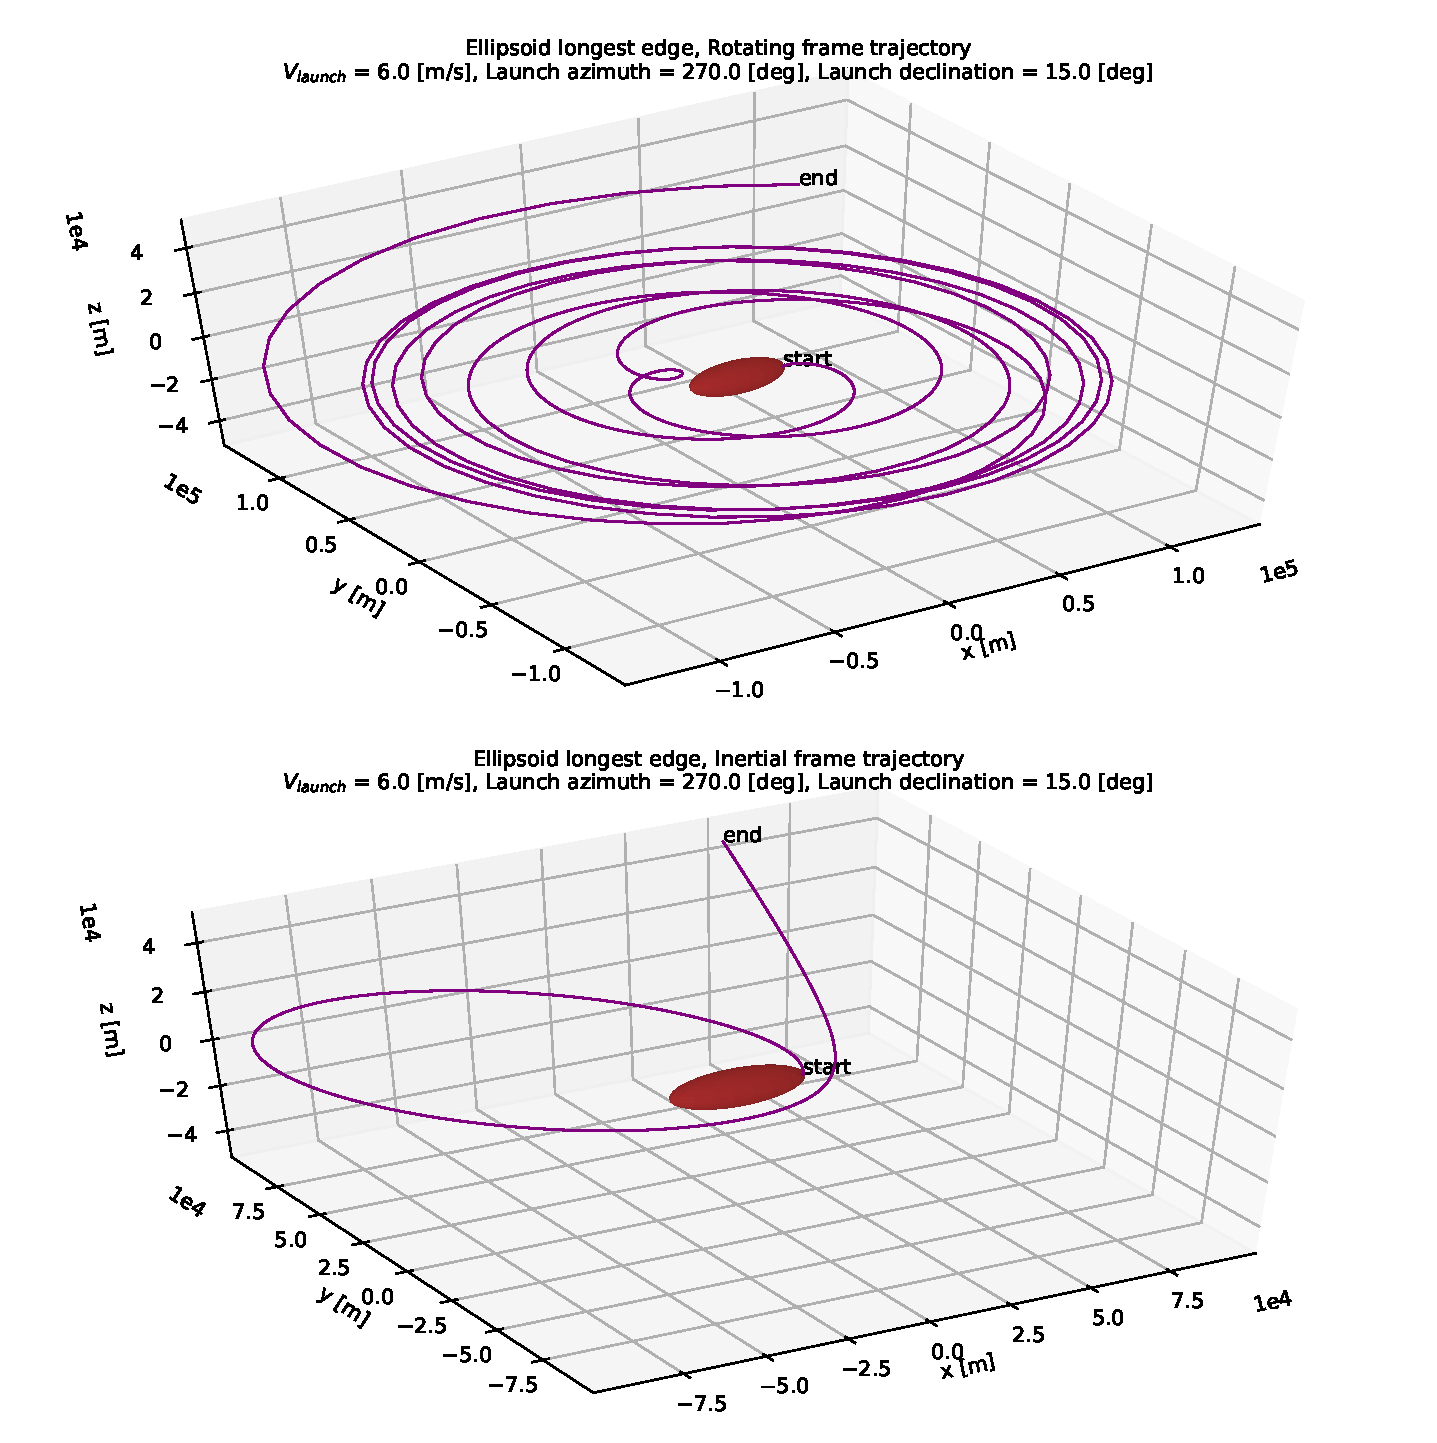
\includegraphics[width=\textwidth, height=0.7\textheight, keepaspectratio=true]{non_conservative_escape_speed/multiRev_3D_trajectory_declination15.pdf}
\caption{3D trajectory in the \gls{ARF} and the \gls{AIF} for launch declination angle \SI{15}{\degree} from \Cref{fig:non_conservative_escape_multiple_qinfinity_single_velocity}.}
\label{fig:3d_traj_declination_15}
\end{figure}
\FloatBarrier
%%%
The animation for the trajectory in \Cref{fig:3d_traj_declination_15} can be found at the web-link given in \Cref{fig:declination_15_animation}. The animation clearly shows the rapid rotation rate of the asteroid which accelerates the particle as it approaches behind it and completes the one and only revolution around the asteroid; having its velocity increased enough to eventually attain a positive energy and escape the asteroid. Thus with the help of gravity perturbations and a fast rotating asteroid, the particle changes from an elliptical orbit to a hyperbolic trajectory leading to its escape. This behavior can not be easily captured just from the initial conditions, as we observed, by the conservative guaranteed escape speed algorithm.
%
\newline\newline
%
An important thing to note here is that the initial condition of the regolith was such that its osculating eccentricity was above 1.0 (but a negative total energy), meaning that at the moment of the launch the regolith was on a hyperbolic trajectory but instantly evolves its orbit into an elliptical one. The reason for this is again the perturbations from a non-uniform gravity field and a rapidly rotating asteroid which keeps osculating the orbit. On the other hand, when we consider a spherical asteroid, the launched particle continues to propagate on the initial trajectory itself because in the absence of perturbations the initial orbital elements do not osculate. Thus for a spherical asteroid, a particle can only escape if the initial orbital elements are such that it is on a parabolic or a hyperbolic trajectory and not otherwise due to a lack of external influences to osculate the orbit. This is why the conservative guaranteed escape speed algorithm works for the spherical asteroid in predetermination of escape situations.
%%%
\begin{figure}[htb]
\centering
\captionsetup{justification=centering}

\includegraphics[width=\textwidth, height=0.1\textheight, keepaspectratio=true]{non_conservative_escape_speed/declination_15_animation.png}
\caption{Scan the QR code to view the 2D trajectory animation in the \gls{AIF} for launch declination angle \SI{15}{\degree} from \Cref{fig:non_conservative_escape_multiple_qinfinity_single_velocity}. The video can also be accessed from the following web-link: \url{https://youtu.be/5l_CAYnjotk}.}
\label{fig:declination_15_animation}
\end{figure}
\FloatBarrier
%%%
%%%
\begin{figure}[htb]
\centering
\captionsetup{justification=centering}
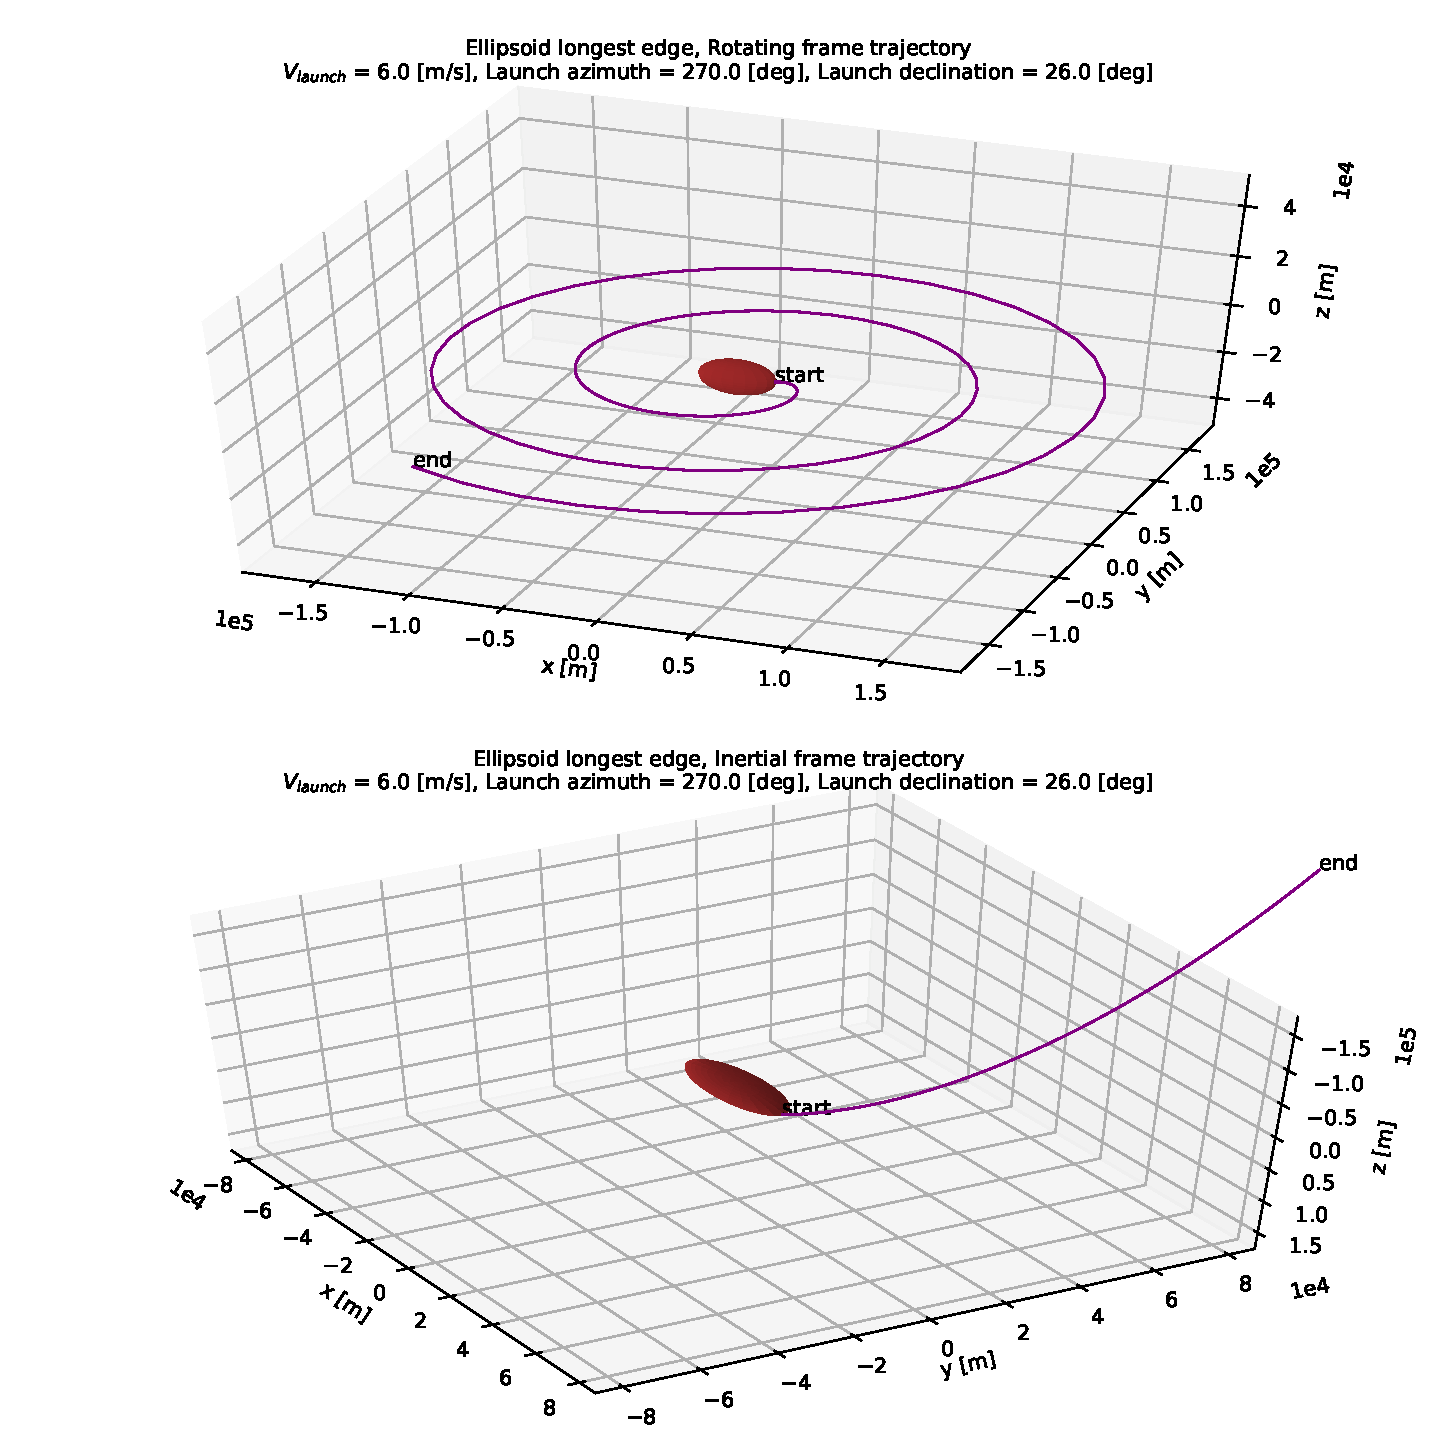
\includegraphics[width=\textwidth, height=0.55\textheight, keepaspectratio=true]{non_conservative_escape_speed/directEscape_3D_trajectory_declination26.pdf}
\caption{3D trajectory expressed in the \gls{ARF} and the \gls{AIF} for a launch declination angle of \SI{26}{\degree} from the normal direction. The particle launch conditions are the same as that used for \protect\Cref{fig:non_conservative_escape_multiple_qinfinity_single_velocity}.}
\label{fig:3d_traj_declination_26}
\end{figure}
\FloatBarrier
%%%
The final aspect that will be discussed in regard to the conservative guaranteed escape speed algorithm is its capacity to distinguish between particles that escape immediately and the ones that take one or more revolutions before escaping, when launched from an irregular body \parencite{scheeres2002fate}. However, we found out that this is only true if the particle is launched from the surface in the normal direction. In that, if the launch speed is lower than the conservative guaranteed escape speed and the particle escapes, then it underwent multiple revolutions. This was observed for multiple particles launched from the longest edge of the \gls{CDE} for launch velocities ranging from 1 to \SI{16}{\metre \per \second}. However, this phenomenon is not observed when the launch direction is not in the normal direction. For example, from \Cref{fig:non_conservative_escape_multiple_qinfinity_single_velocity}, the launch declination angle of \SI{26}{\degree} results in a direct escape scenario, even though the launch velocity is below the conservative guaranteed escape speed algorithm. The 3D trajectory for this case is shown in \Cref{fig:3d_traj_declination_26}.
%
\newline\newline
%
Thus, it is imperative to understand that with just a non-uniform gravity field and a relatively fast rotating asteroid, the dynamics for orbiting regolith become intangible enough such that predetermination of orbital behavior and final fate of the regolith can not be explained by simple analytical methods. We attempted to explain the complex behavior by deriving a different guaranteed escape speed algorithm, however, the method failed completely. We realize now that a numerical simulation method is a relatively better approach to understand the orbital dynamics of regolith lofted from an asteroid.


\chapter{Dynamics Without Solar Perturbations}
\label{chap:dynamics_without_solar_perturbations}
\graphicspath{{Results/}}

In this chapter, we will analyze the orbital motion of regolith in presence of a non-uniform gravity field, i.e. the \gls{CDE} gravity model, but in the absence of all Solar perturbations. We try to understand the general behavior of regolith under such circumstances first so that we can later understand the effect of adding Solar perturbations.

\section{Simulation Setup}
\label{sec:simulation_setup_noSP}
Since the aim is to understand the general characteristic behavior of regolith orbiting an elongated asteroid with a non-uniform gravity field, we chose the launch site to be on the longest edge of the asteroid, i.e. Longitude and Latitude both \SI{0}{\degree}. This launch site was chosen because it offers an easy and intuitive demarcation of particles being launched in or against the direction of asteroid's rotation. This demarcation is non-intuitive for any other general launch site, such as the one on the leading edge of the asteroid.
%
\newline\newline
%
Multiple particles are launched from the surface, forming the shape of a cone. The launch declination angle was fixed to be a general value of \SI{45}{\degree} and the launch azimuth angle was varied from 0 to \SI{359}{\degree}, thereby launching regolith in every possible direction for a given declination value. The launch velocity was varied from \SI{1}{\metre \per \second} to \SI{16}{\metre \per \second}. Thus, in total 5760 particles were launched and simulated, each with unique initial conditions.

\section{Final Fate Characteristics}
\label{sec:final_fate_characteristics_noSP}
The results presented in this section are a direct consequence of an attempt to understand any link between how a particle was launched and what their final outcome is. This, ofcourse, was done in the absence of any external disturbance apart from the non-uniform gravity field so as to reduce the number of contributing factors for uncertainty. The initial intention of performing this part of the research was to discover the said link(s) through investigative methods and then later exploit it for space exploration activities.

\subsection{General Behavior}
\label{subsec:general_behavior_noSP}
We'll begin by first looking at the different final outcomes and understand them as is by observing certain underlying parametric values. \Cref{fig:final_fate_hist_noSP} depicts the final fates acquired by particles for each of the launch velocities (expressed in the \gls{ARF}). At the extreme ends of the launch velocity range, we can see that the final fate is absolute. If the launch velocity is extremely small then all particles just re-impact the surface and if the velocity is too large, then the particles simply escape. For all other launch velocities in between, the distribution of final fates is mixed, with re-impact gaining more prominence over escape if the velocity is relatively lower and vice-versa.
%%%
\begin{figure}[htb]
\centering
\captionsetup{justification=centering}
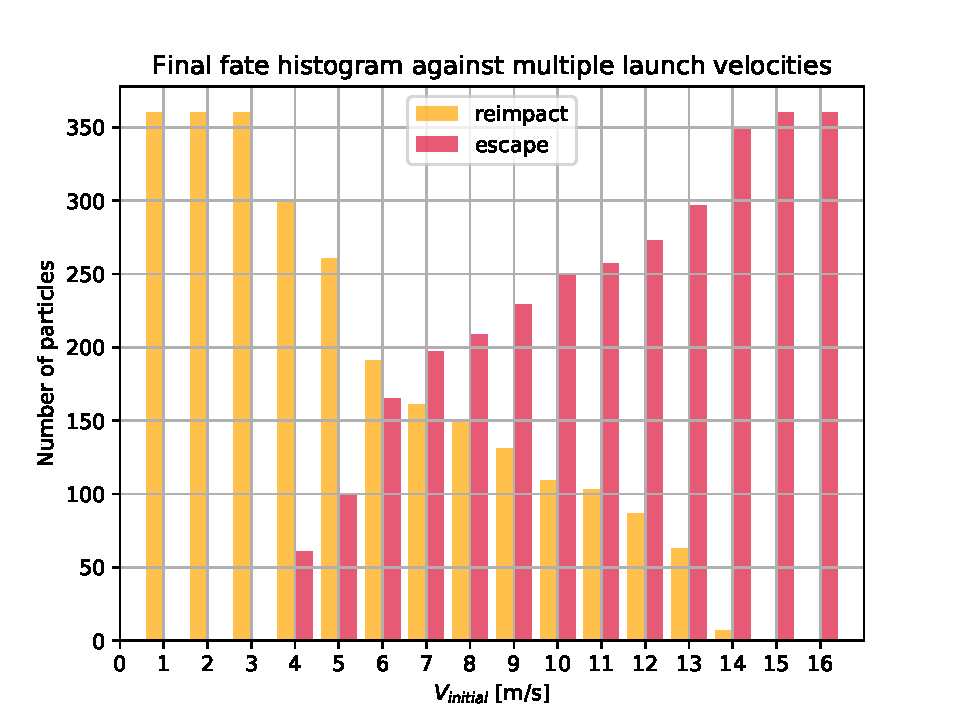
\includegraphics[width=\textwidth, height=0.4\textheight, keepaspectratio=true]{Images/longest_edge_no_perturbations/final_fate_histogram_all_velocities.pdf}
\caption{A histogram plot depicting the different final outcomes against all launch velocities. The latter are expressed with respect to the \gls{ARF}. The values on the y-axis are representative of the number of particles that acquired each of the distinctive final fates for every launch velocity and do not represent the launch azimuth values.}
\label{fig:final_fate_hist_noSP}
\end{figure}
\FloatBarrier
%%%
An important thing to notice is the lack of particles with temporary capture as their final fate in \Cref{fig:final_fate_hist_noSP}. Recall from \Cref{sec:assumptions} that each particle or regolith is simulated for a maximum of 270 Earth days. So upon closer examination of the output databases, it was found that their are a few particles which did not re-impact or escape at the end of the 270 days simulation. These particles were not temporarily captured by the asteroid, but instead, each particle was found to be on a single orbit with extremely large semi-major axis and eccentricity. Soon after launch these particles went extremely far away from the asteroid, but still weakly bounded to it through gravity, and never returned back in the vicinity of the asteroid within the total time set for the simulation. These are not capture orbits since the definition requires them to perform multiple orbital revolutions around the asteroid for hundreds of days. Moreover, these are the particles that eventually get whisked away from the asteroid's gravitational pull because of Solar perturbations (observed when simulations were run with \gls{SRP} and \gls{STBE}).
%
\newline\newline
%
\Cref{fig:final_fate_time_noSP} shows the total time taken by regolith, launched with different launch conditions, to meet their respective final fates. The plot shows that, for the same final fate, its not not just the launch velocity but the direction of launch as well that can have a significant impact on the total time it takes to meet a given fate. For a given launch velocity and say the escape case, we can see that if the particle is launched in the direction of the rotation (for example, azimuth = \SI{270}{\degree}), then it gets an extra boost from the asteroid's rotation and results in taking lesser time to escape. This is relative to being launched in a direction opposite to the asteroid's rotation (for example, azimuth = \SI{90}{\degree}), where the particle gets slowed down as its direction of motion is opposing the direction of the gravitational force and hence takes more time to escape for the same initial launch velocity.
%%%
\begin{figure}[htb]
\centering
\captionsetup{justification=centering}
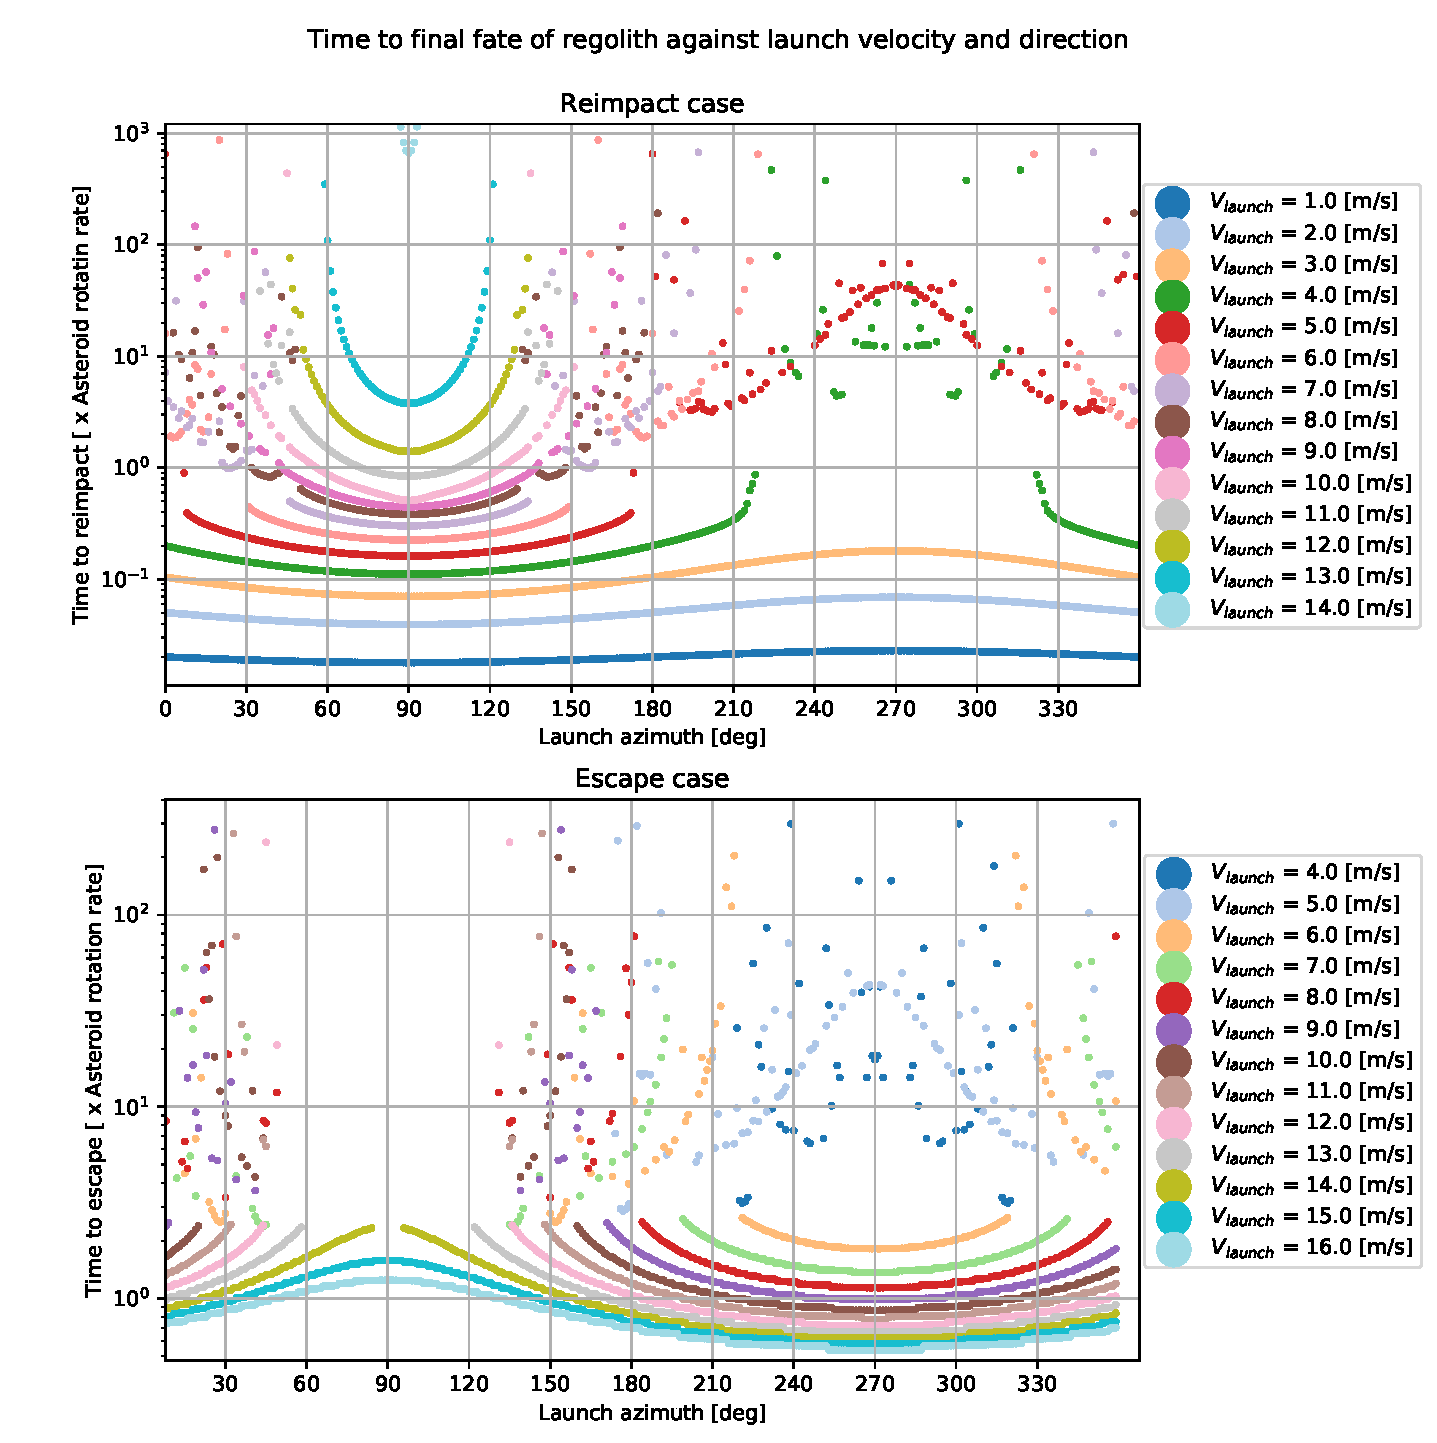
\includegraphics[width=\textwidth, height=0.6\textheight, keepaspectratio=true]{Images/longest_edge_no_perturbations/time_to_final_fate_all_velocities.pdf}
\caption{Plot depicting the total time taken by regolith to meet their respective final outcomes, as a function of the launch azimuth and the launch velocity. The time values are mentioned as a multiple of the asteroid rotation rate which is 5.27 hours.}
\label{fig:final_fate_time_noSP}
\end{figure}
\FloatBarrier
%%%
This situation with launch direction and time to final fate gets reversed when we consider the case of re-impact. Thus for the same velocity, when launched in the direction of asteroid's rotation, the particle tends to go further away from the asteroid because of an excess velocity provided by the rotation which then results in more time for the particle to come back and re-impact the surface. This directional behavior, for escape or re-impact, is seen for majority of the cases, however, it can not be generalized as we do see some exceptions. These exceptions are observed only for the cases where the launch velocity results in both escape and re-impact situations. The most notable example for this is the escape scenarios for the launch velocity of \SI{4}{\metre \per \second}. For the current example, escape occurs only when the launch azimuth is favorable, i.e. when the particles is launched in the rotational direction, in addition to a complex interaction with the fast rotating asteroid and irregular gravity field. So for the example of \SI{4}{\metre \per \second}, escape occurs not because the velocity is inherently high enough but because of the interaction with the asteroid which is why a chaotic behavior for it is observed in \Cref{fig:final_fate_time_noSP}.
%
\newline\newline
%
We now look at the velocity extremes in \Cref{fig:final_fate_hist_noSP} which result either only in a re-impact or escape, and observe their orbital time in \Cref{fig:final_fate_time_noSP}. It is observed that the time to achieve the respective final fates is extremely small and mostly in fractions of the asteroid's rotation rate. This means that these particles don't spend enough time in orbit to get affected by the non-uniform gravity field or the asteroid's rotation and hence show no exceptional behavior as discussed before.
%%%
\begin{figure}[htb]
\centering
\captionsetup{justification=centering}
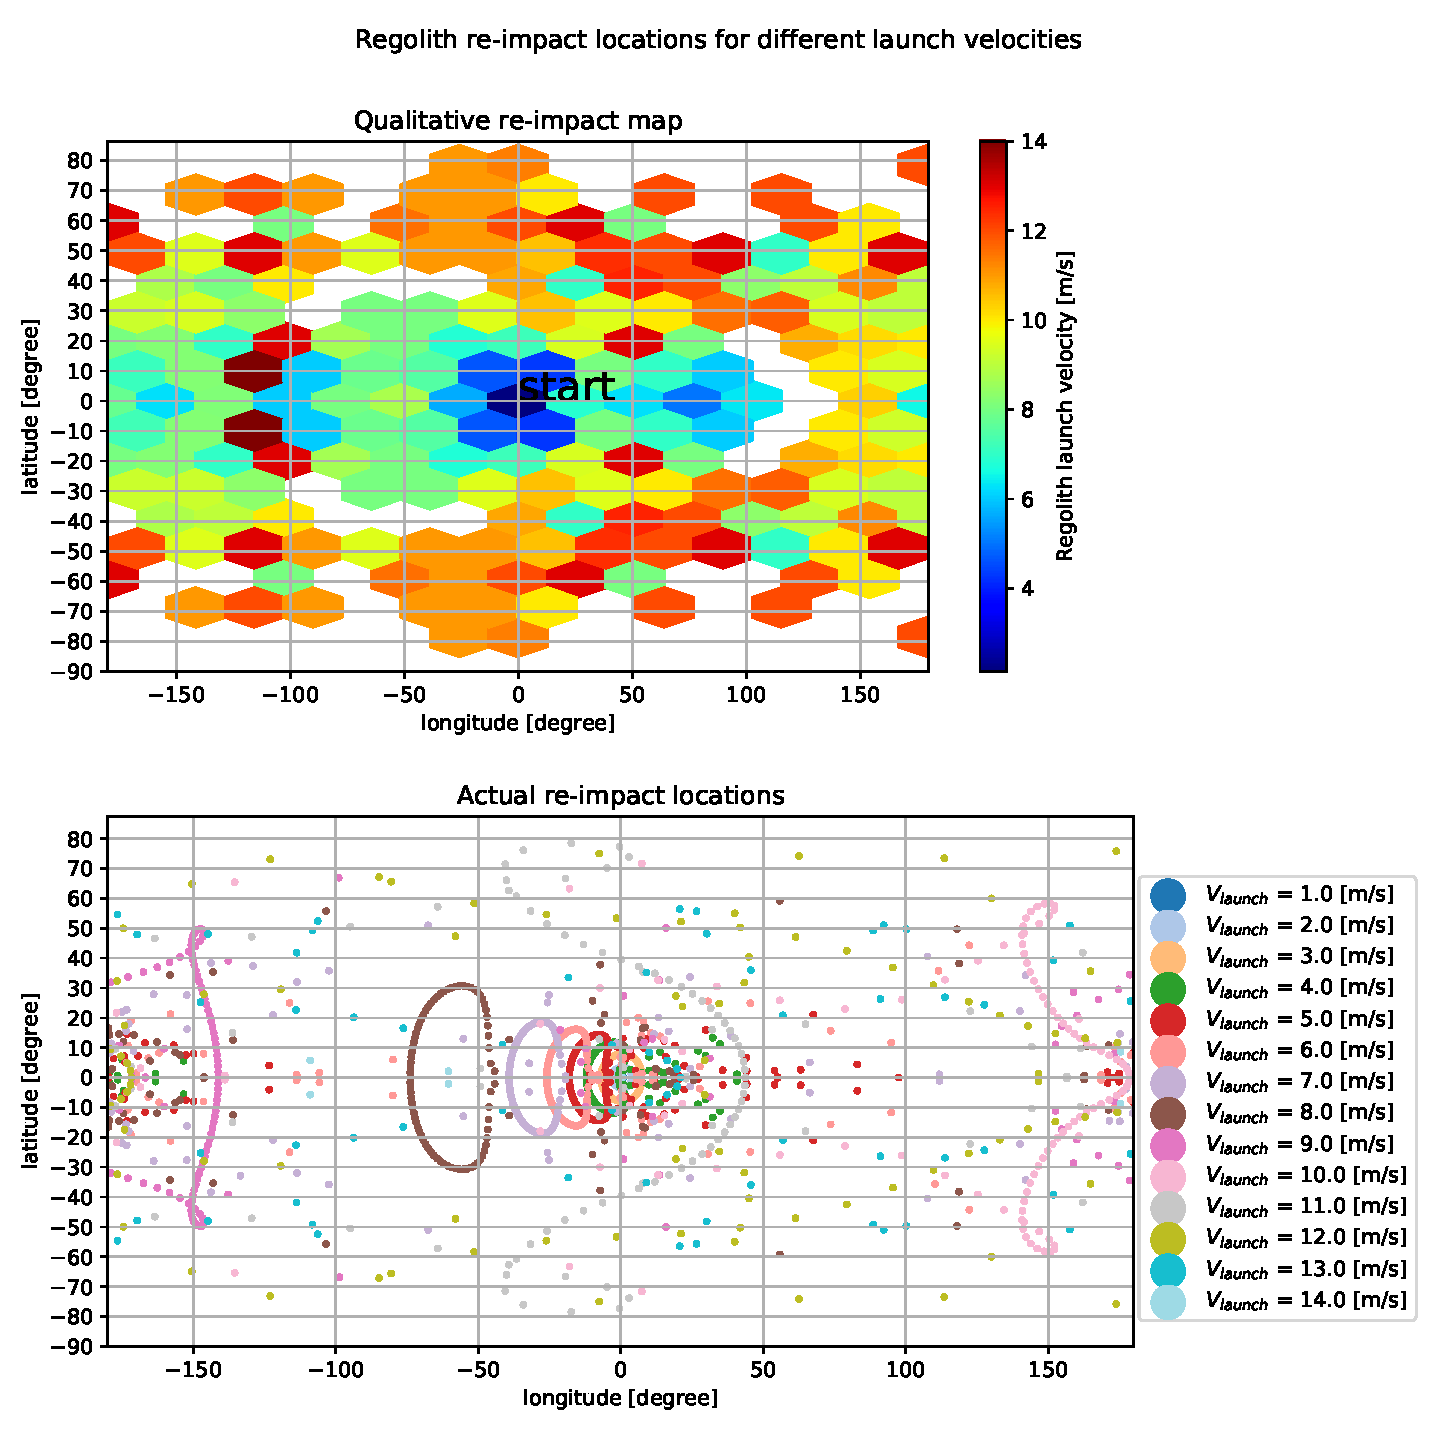
\includegraphics[width=\textwidth, height=0.6\textheight, keepaspectratio=true]{Images/longest_edge_no_perturbations/crash_map_all_velocities.pdf}
\caption{Regolith re-impact locations marked for all launch velocities that eventually lead to it. A qualitative map is shown as well that provides a general idea on re-impact locations and is color coded based on the regolith launch velocity.}
\label{fig:crashmap_all_noSP}
\end{figure}
\FloatBarrier
%%%

\subsection{Re-impact behavior}
This section will discuss certain characteristic behavior that is specific to the re-impact scenario. \Cref{fig:crashmap_all_noSP} shows a map of re-impact locations on the surface of the asteroid for all launch velocities that led to this particular fate. The distinction due to launch azimuth is not plotted explicitly. The qualitative map in the plot is simply a 2D histogram plot with hexagonal shaped bins. These bins don't represent the amount of particles within a given location but instead represent the initial launch velocities that led to a re-impact in that location. From the qualitative map, we can observe that particles launched with the lowermost velocities mostly re-impact very close to the launch site itself. The intermediate velocities seems to confine the re-impact locations within the \SI{-30}{\degree} to \SI{+30}{\degree} latitude range and lie mostly on the West of the launch site. And finally, the higher velocity range cause the particle to re-impact mostly on the upper latitudes in both the North and the South. Thus the qualitative map gives an excellent description of how the re-impact locations change with increasing launch velocities. The map with the actual re-impact locations in \Cref{fig:crashmap_all_noSP} shows that the bulk of all re-impacted particles lie around the two longest edges of the asteroid. Everywhere in between has a very scarce distribution of particles. A pattern in the re-impact location becomes apparent if one visualizes the launch azimuth angles, especially for the lower launch velocity range and is discussed shortly.
%%%
\begin{figure}[htb]
\centering
\captionsetup{justification=centering}
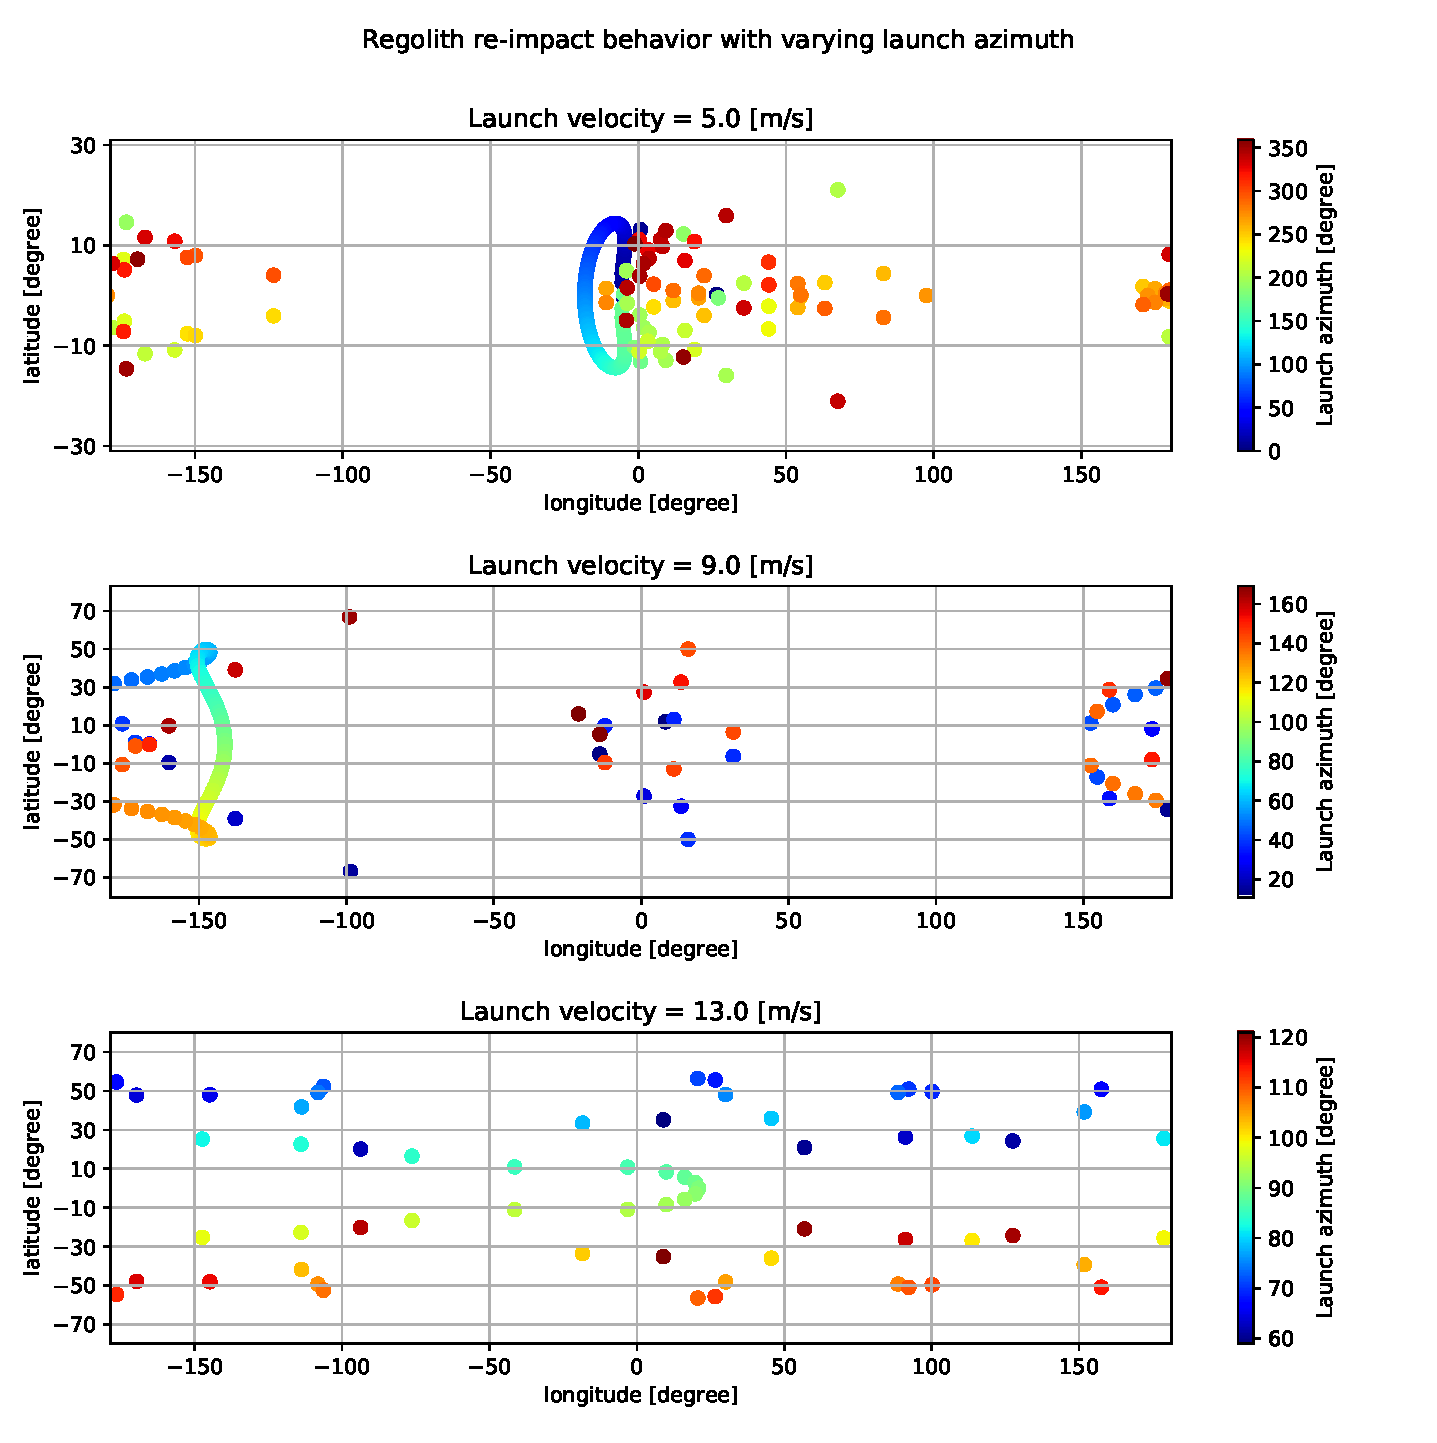
\includegraphics[width=\textwidth, height=0.6\textheight, keepaspectratio=true]{Images/longest_edge_no_perturbations/re-impact_behavior_with_azimuth.pdf}
\caption{Single velocity re-impact location maps for three different velocities. The re-impact locations are color coded based on the launch azimuth.}
\label{fig:crashmap_launchAzimuth_noSP}
\end{figure}
\FloatBarrier
%%%
We look a bit more in detail into the re-impact location map for three different velocities. These velocities are chosen such that, by studying them, we can estimate the behavior for the low, intermediate and high launch velocities. In addition to this, we also look at the effect of the launch direction on re-impact location and see if there is a link between them or if it is all chaotic.
%
\newline\newline
%
For the launch velocity of \SI{5}{\metre \per \second}, the re-impact locations corresponding to launch azimuth angles that are against the asteroid's rotational direction (more specifically \SI{7}{\degree} to \SI{173}{\degree})\footnote{Trajectories for launch azimuths \SI{1}{\degree} to \SI{6}{\degree} and \SI{174}{\degree} to \SI{179}{\degree} get assisted by the fast rotating asteroid which results in them entering escape trajectories}, form a distinct curve West of the launch location. These are the particles that soon after launch, re-impact the surface without completing even a single orbit because their energy is reduced significantly enough by the opposing direction of the gravity field. And since the initial launch velocity was inherently small, these particles are not able to reach far away from the launch site either. Launch azimuths \SI{0}{\degree} and \SI{180}{\degree} are not directly against or into the asteroid's rotational direction and the corresponding particles complete multiple revolutions before re-impacting the asteroid's surface. Their re-impact location is \SI{0.2}{\degree} latitude and \SI{26.6}{\degree} longitude and can be seen in \Cref{fig:crashmap_launchAzimuth_noSP}. The remaining launch azimuth angles, i.e. the ones that launch the particle in the asteroid's rotational direction \footnote{Not all of these result in re-impact, a few of these also result in an escape scenario but that is irrelevant for the discussion at hand}, results in a more oddly distributed re-impact locations. The asteroid's rotation assists the launch such that the particles complete one or more orbital revolutions (observed from individual trajectory plots) before re-impacting the surface. This is why for these azimuth angles, the re-impacted particles are not evenly distributed in a smooth curve on the East side of the launch site as the trajectories are not simply ballistic. The re-impact locations in 3D for this launch velocity are shown in \Cref{fig:crashmap_3d_5ms_noSP}.
%%%
\begin{figure}[htb]
\centering
\captionsetup{justification=centering}
\subfloat[]{
    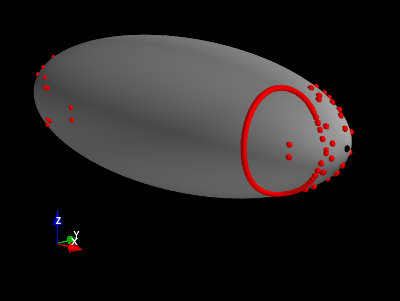
\includegraphics[width=0.5\textwidth, height=0.5\textheight, keepaspectratio=true]{Images/longest_edge_no_perturbations/5ms_crashMap_view1.png}
    \label{fig:crash_3d_5ms_view1}
}
\subfloat[]{
    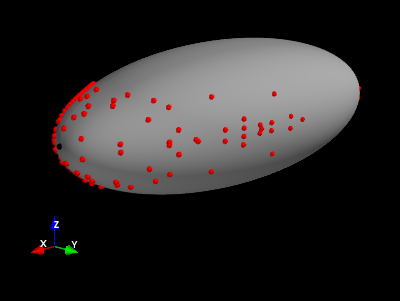
\includegraphics[width=0.5\textwidth, height=0.5\textheight, keepaspectratio=true]{Images/longest_edge_no_perturbations/5ms_crashMap_view2.png}
    \label{fig:crash_3d_5ms_view2}
}

\subfloat[]{
    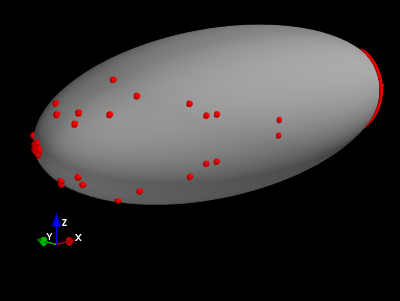
\includegraphics[width=0.5\textwidth, height=0.5\textheight, keepaspectratio=true]{Images/longest_edge_no_perturbations/5ms_crashMap_view3.png}
    \label{fig:crash_3d_5ms_view3}
}
\subfloat[]{
    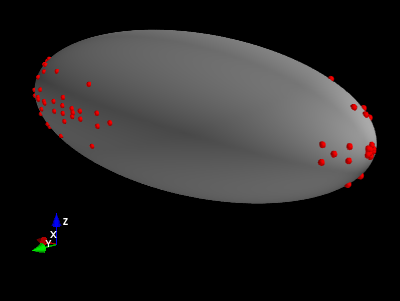
\includegraphics[width=0.5\textwidth, height=0.5\textheight, keepaspectratio=true]{Images/longest_edge_no_perturbations/5ms_crashMap_view4.png}
    \label{fig:crash_3d_5ms_view4}
}
\caption{3D view, from four different angles, of regolith re-impact locations for particles launched with a velocity of \SI{5}{\metre \per \second}. The red points represent the re-impact sites and the singular black dot represents the launch site.}
\label{fig:crashmap_3d_5ms_noSP}
\end{figure}
\FloatBarrier
%%%
Consider the re-impact locations in \Cref{fig:crashmap_launchAzimuth_noSP} for the launch velocity of \SI{9}{\metre\per\second}. Note that, for this velocity, the launch azimuth angles that result in a re-impact are only the ones which launch the particle in a direction opposite to that of the asteroid's rotation \footnote{Not all the angles within this range correspond to a re-impact situation and some result in an escape as well but the latter is not relevant to the discussion at hand}. Within this range of azimuth angles, the lowermost and the uppermost angles comprise of trajectories that are either ballistic or comprise of one or more orbital revolutions. In case of the ballistic trajectories, we do not see the behavior as we saw for the launch velocity case of \SI{5}{\metre\per\second} where the particles neatly lined up on the West side of the launch site. For the current case, the launch velocity magnitude is inherently high. We observed a particle which took the least amount of time to re-impact and also had a ballistic trajectory, and found that the asteroid had rotated a little more than \SI{315}{\degree} when the particle re-impacted the surface but on the far East end of the asteroid. Since the launch velocity is inherently high, the particle was able to achieve a high enough altitude during which the asteroid had achieved a significant amount of rotation on its own axis, which led to the aforementioned situation.
%
\newline\newline
%
There is a very distinct collection of re-impact points (the blue-green-orange curve) on the West side of the launch point, in \Cref{fig:crashmap_launchAzimuth_noSP} for the velocity of \SI{9}{\metre\per\second} and belongs to the azimuth angles from \SI{46}{\degree} to \SI{136}{\degree}. The corresponding trajectories are all ballistic in nature and impact the surface relatively sooner after launch. Since the launch velocity is inherently high, unlike in the case of \SI{5}{\metre\per\second}, these particles are able to re-impact a bit further away from the launch site. This is clearly visible in \Cref{fig:crashmap_launchAzimuth_noSP}. For the case of \SI{9}{\metre\per\second}, the 3D view of all re-impact locations is shown in \Cref{fig:crashmap_3d_9ms_noSP}.
%%%
\begin{figure}[htb]
\centering
\captionsetup{justification=centering}
\subfloat[]{
    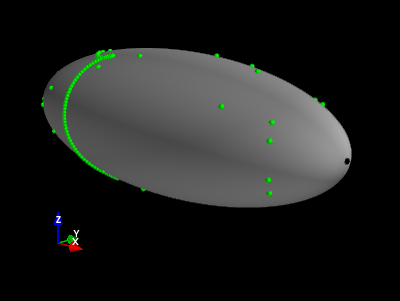
\includegraphics[width=0.5\textwidth, height=0.5\textheight, keepaspectratio=true]{Images/longest_edge_no_perturbations/9ms_crashMap_view1.png}
    \label{fig:crash_3d_9ms_view1}
}
\subfloat[]{
    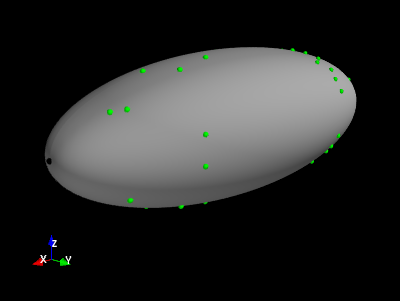
\includegraphics[width=0.5\textwidth, height=0.5\textheight, keepaspectratio=true]{Images/longest_edge_no_perturbations/9ms_crashMap_view2.png}
    \label{fig:crash_3d_9ms_view2}
}

\subfloat[]{
    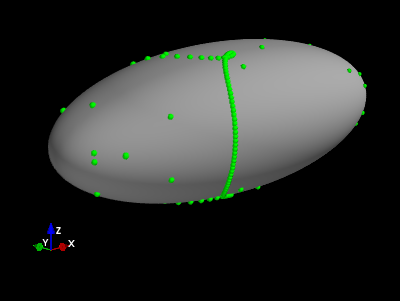
\includegraphics[width=0.5\textwidth, height=0.5\textheight, keepaspectratio=true]{Images/longest_edge_no_perturbations/9ms_crashMap_view3.png}
    \label{fig:crash_3d_9ms_view3}
}
\subfloat[]{
    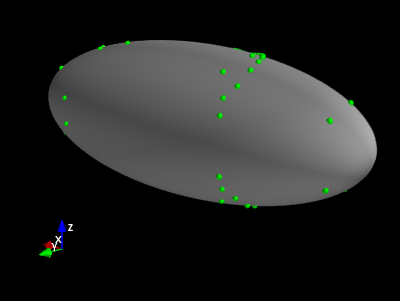
\includegraphics[width=0.5\textwidth, height=0.5\textheight, keepaspectratio=true]{Images/longest_edge_no_perturbations/9ms_crashMap_view4.png}
    \label{fig:crash_3d_9ms_view4}
}
\caption{3D view, from four different angles, of regolith re-impact locations for particles launched with a velocity of \SI{9}{\metre \per \second}. The green points represent the re-impact sites and the singular black dot represents the launch site.}
\label{fig:crashmap_3d_9ms_noSP}
\end{figure}
\FloatBarrier
%%%
Similarly, for the launch case of \SI{13}{\metre\per\second} in \Cref{fig:crashmap_launchAzimuth_noSP}, we first notice that the window or range of launch azimuth angles has reduced further. All particle trajectories, in this case, are ballistic in nature and we do not witness a continuous line of re-impact locations, as opposed to that in the case of \SI{5}{\metre\per\second} and \SI{9}{\metre\per\second}. When launched at \SI{13}{\metre\per\second}, the ballistic trajectories are not short lived, that re-impact the surface soon after launch \footnote{Soon after launch, here, refers to the fact that the ballistic trajectories re-impacted the surface before the asteroid could complete even a single rotation on its own axis}, which would have allowed a continuous curve on surface to be formed. Since for the current case the launch velocity has a sufficiently larger magnitude, the particles are lofted into even higher altitude trajectories, taking more time to traverse. This is the fundamental difference with the other two velocity cases, as here the asteroid performs several rotations on its axis before the particles re-impact. Thus the ballistic re-impact trajectories for launch velocity of \SI{13}{\metre\per\second} shows similar behavior as that of the multi-orbital revolution cases of \SI{5}{\metre\per\second} and \SI{9}{\metre\per\second}. The re-impact locations in 3D are shown in \Cref{fig:crashmap_3d_13ms_noSP}.
%%%
\begin{figure}[htb]
\centering
\captionsetup{justification=centering}
\subfloat[]{
    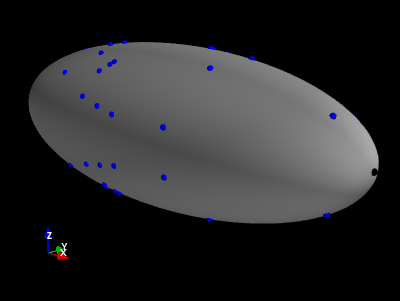
\includegraphics[width=0.5\textwidth, height=0.5\textheight, keepaspectratio=true]{Images/longest_edge_no_perturbations/13ms_crashMap_view1.png}
    \label{fig:crash_3d_13ms_view1}
}
\subfloat[]{
    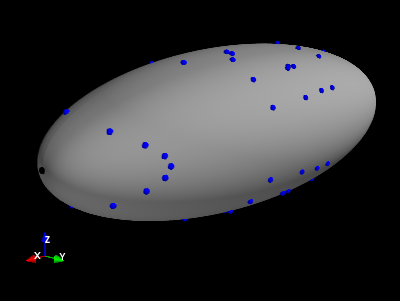
\includegraphics[width=0.5\textwidth, height=0.5\textheight, keepaspectratio=true]{Images/longest_edge_no_perturbations/13ms_crashMap_view2.png}
    \label{fig:crash_3d_13ms_view2}
}

\subfloat[]{
    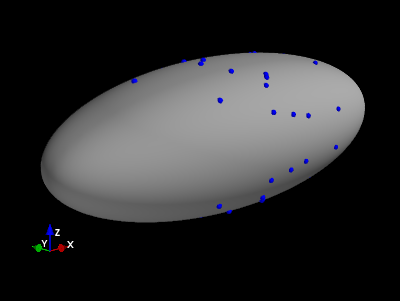
\includegraphics[width=0.5\textwidth, height=0.5\textheight, keepaspectratio=true]{Images/longest_edge_no_perturbations/13ms_crashMap_view3.png}
    \label{fig:crash_3d_13ms_view3}
}
\subfloat[]{
    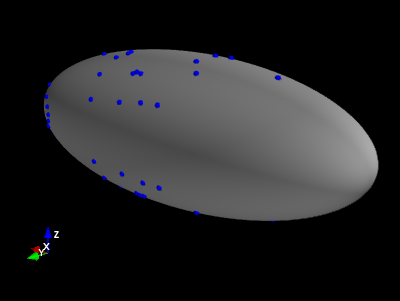
\includegraphics[width=0.5\textwidth, height=0.5\textheight, keepaspectratio=true]{Images/longest_edge_no_perturbations/13ms_crashMap_view4.png}
    \label{fig:crash_3d_13ms_view4}
}
\caption{3D view, from four different angles, of regolith re-impact locations for particles launched with a velocity of \SI{13}{\metre \per \second}. The blue points represent the re-impact sites and the singular black dot represents the launch site.}
\label{fig:crashmap_3d_13ms_noSP}
\end{figure}
\FloatBarrier
%%%
Thus, for lower launch velocities, a continuous curve of re-impact locations can be linked to the launch direction which in our case is the launch azimuth angle \footnote{The launch declination angle for our simulation was kept constant}. But the same can not be said for higher launch velocities. Another intriguing observation in \Cref{fig:crashmap_launchAzimuth_noSP} is made for the launch velocity of \SI{5}{\metre\per\second}. We see that the particle launched with azimuth angle of \SI{90}{\degree} goes further away than, for example, a particle launched with an azimuth angle of \SI{10}{\degree}. This happens even though the former launch case will experience more resistance in launch since it is directly opposite to the asteroid's rotational direction. The reason for this is simple and becomes apparent if one looks at the trajectory plots shown in \Cref{fig:5ms_traj_90and10_azim_noSP}.

\subsection{Escape Behavior}
\label{subsec:escape_behavior_noSP}
We now present a brief discussion on the particles that resulted in an escape situation, and do so for the same launch velocities used for explaining the re-impact scenarios. For these launch velocities, \Cref{fig:hev_escapeHist_noSP} shows the \gls{HEV} for all escaped regolith.
%%%
\begin{figure}[htb]
\centering
\captionsetup{justification=centering}
\subfloat[]{
    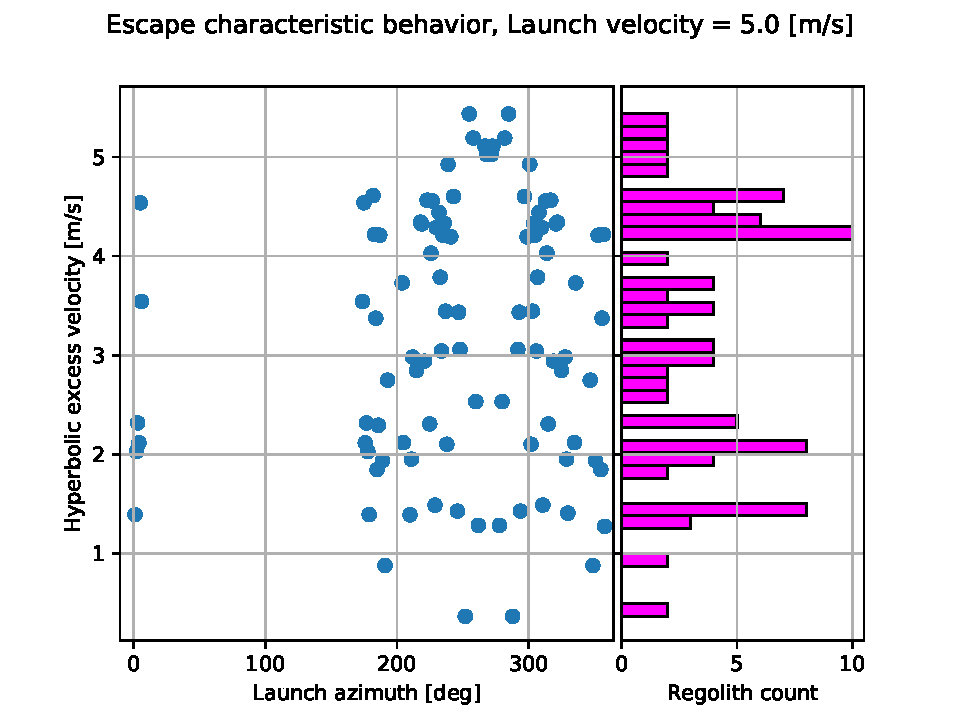
\includegraphics[width=0.5\textwidth, height=0.5\textheight, keepaspectratio=true]{Images/longest_edge_no_perturbations/escape_behavior_5ms.pdf}
    \label{fig:hev_escapeHist_5ms_noSP}
}
\subfloat[]{
    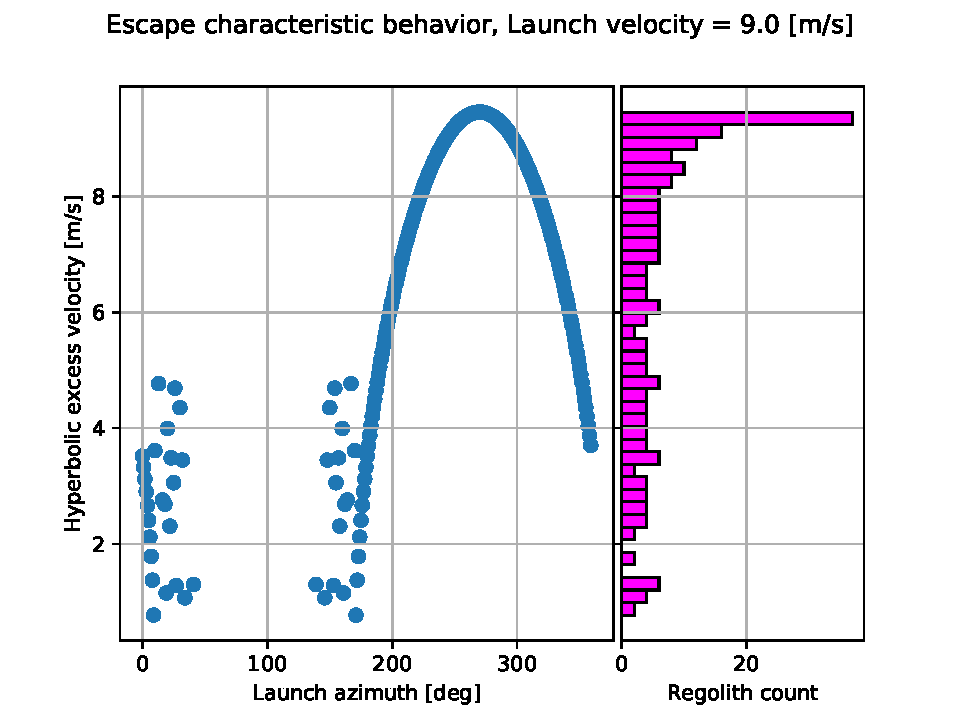
\includegraphics[width=0.5\textwidth, height=0.5\textheight, keepaspectratio=true]{Images/longest_edge_no_perturbations/escape_behavior_9ms.pdf}
    \label{fig:hev_escapeHist_9ms_noSP}
}

\subfloat[]{
    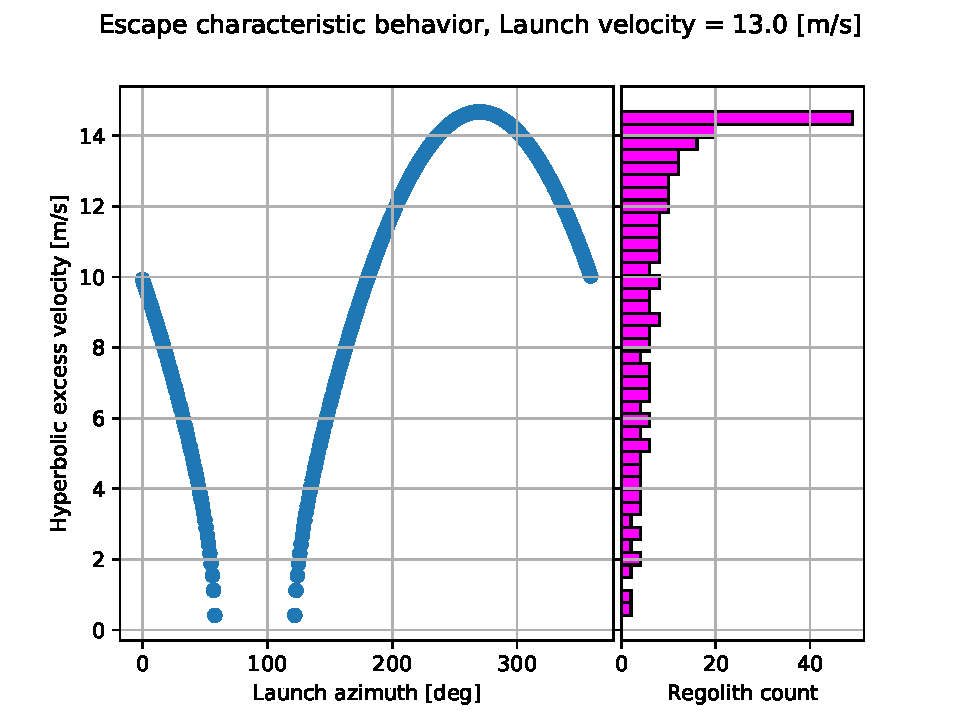
\includegraphics[width=0.5\textwidth, height=0.5\textheight, keepaspectratio=true]{Images/longest_edge_no_perturbations/escape_behavior_13ms.pdf}
    \label{fig:hev_escapeHist_13ms_noSP}
}
\caption{Hyperbolic escape velocity versus launch azimuth for three different launch velocity cases. The histogram bars in each plot depicts the number of regolith for the various hyperbolic excess velocities on the y-axis.}
\label{fig:hev_escapeHist_noSP}
\end{figure}
\FloatBarrier
%%%
As the velocity increases from \SI{5}{\metre\per\second} to \SI{13}{\metre\per\second}, we see that the distribution of particles, based on their \gls{HEV}, becomes less and less random and more streamlined. There is a link between how the particles are distributed with \gls{HEV} and the way they escape. To understand this, we take the example of \SI{9}{\metre\per\second} and look at all escape cases from below \SI{100}{\degree} in launch azimuth. A zoomed in version of the corresponding data points from \Cref{fig:hev_escapeHist_9ms_noSP} is shown in \Cref{fig:hev_9ms_lowerAzimuths_noSP}. In the latter, we can see that for launch azimuths from \SI{0}{\degree} to \SI{9}{\degree}, the \gls{HEV} uniformly reduces and beyond that all other data points are randomly distributed. The distinction between the two becomes apparent when we look at the osculating energy and eccentricity for all these data points, as shown in \Cref{fig:energy_ecc_escape_9ms_noSP}.
%%%
\begin{figure}[htb]
\centering
\captionsetup{justification=centering}
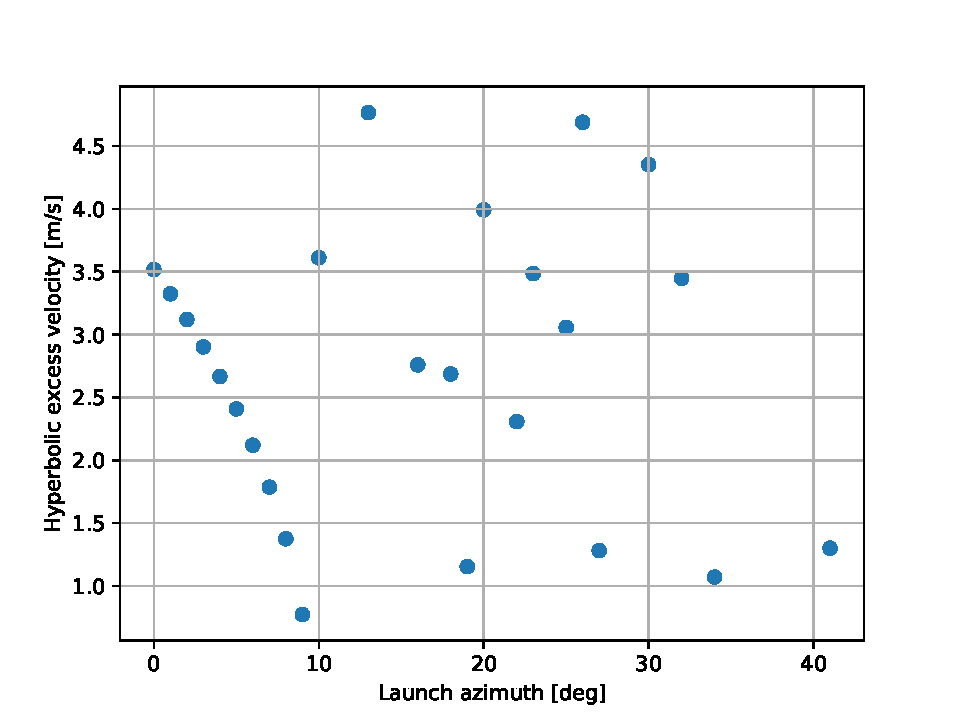
\includegraphics[width=\textwidth, height=0.3\textheight, keepaspectratio=true]{Images/longest_edge_no_perturbations/escape_hev_9ms_lowerAzimuth.pdf}
\caption{Zoomed in data points for azimuth angles below \SI{100}{\degree} from \protect\Cref{fig:hev_escapeHist_9ms_noSP}.}
\label{fig:hev_9ms_lowerAzimuths_noSP}
\end{figure}
\FloatBarrier
%%%
So for the data points with uniformly reducing \gls{HEV} values, we observe that the energy never becomes negative and the eccentricity always stays above 1.0, which means that the corresponding regoliths are on an escape trajectory immediately after launch. It doesn't take a gravity assist from the fast rotating asteroid to put these regolith on an escape route. This is an important distinction against the randomly distributed data points in \Cref{fig:hev_9ms_lowerAzimuths_noSP}.For the latter, from the eccentricity and energy curves, we can witness that the particles briefly enter bounded orbits around the asteroid but eventually escape with a sudden increase in energy (becoming positive) and eccentricity (going above 1.0). This happens because, after launch, the particle trajectories get gravity assist from the asteroid that is sufficient to put the particle on an escape route. What was shown here for an example of \SI{9}{\metre\per\second} was not an isolated case and was found to be true for other launch velocities as well, but their results are not shown here for brevity. Thus, just by looking at the \gls{HEV} plot, we can now determine which launch azimuths led to an immediate escape and which ones required gravity assist from the asteroid to escape. The trajectory plots for a few launch azimuths that highlight this distinction is shown in \Cref{fig:escape_example_traj_9ms_noSP}.
%%%
\begin{figure}[htb]
\centering
\captionsetup{justification=centering}
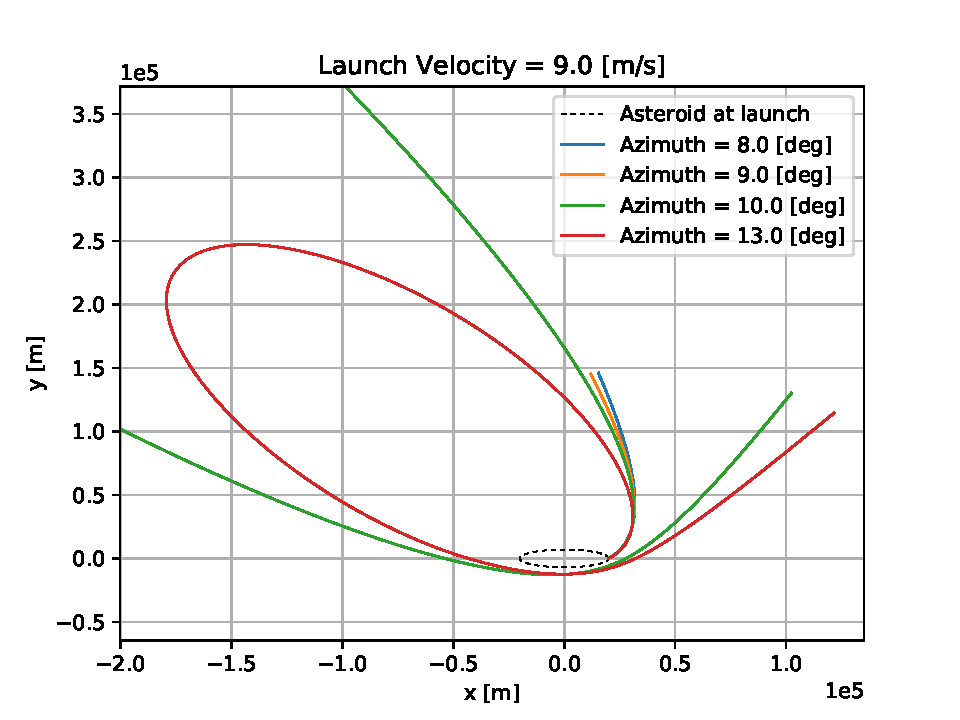
\includegraphics[width=\textwidth, height=0.3\textheight, keepaspectratio=true]{Images/longest_edge_no_perturbations/9ms_escape_example_trajectories.pdf}
\caption{Example escape case trajectory plots for a few launch azimuths.}
\label{fig:escape_example_traj_9ms_noSP}
\end{figure}
\FloatBarrier
%%%
%%%
\begin{figure}[htb]
\centering
\captionsetup{justification=centering}
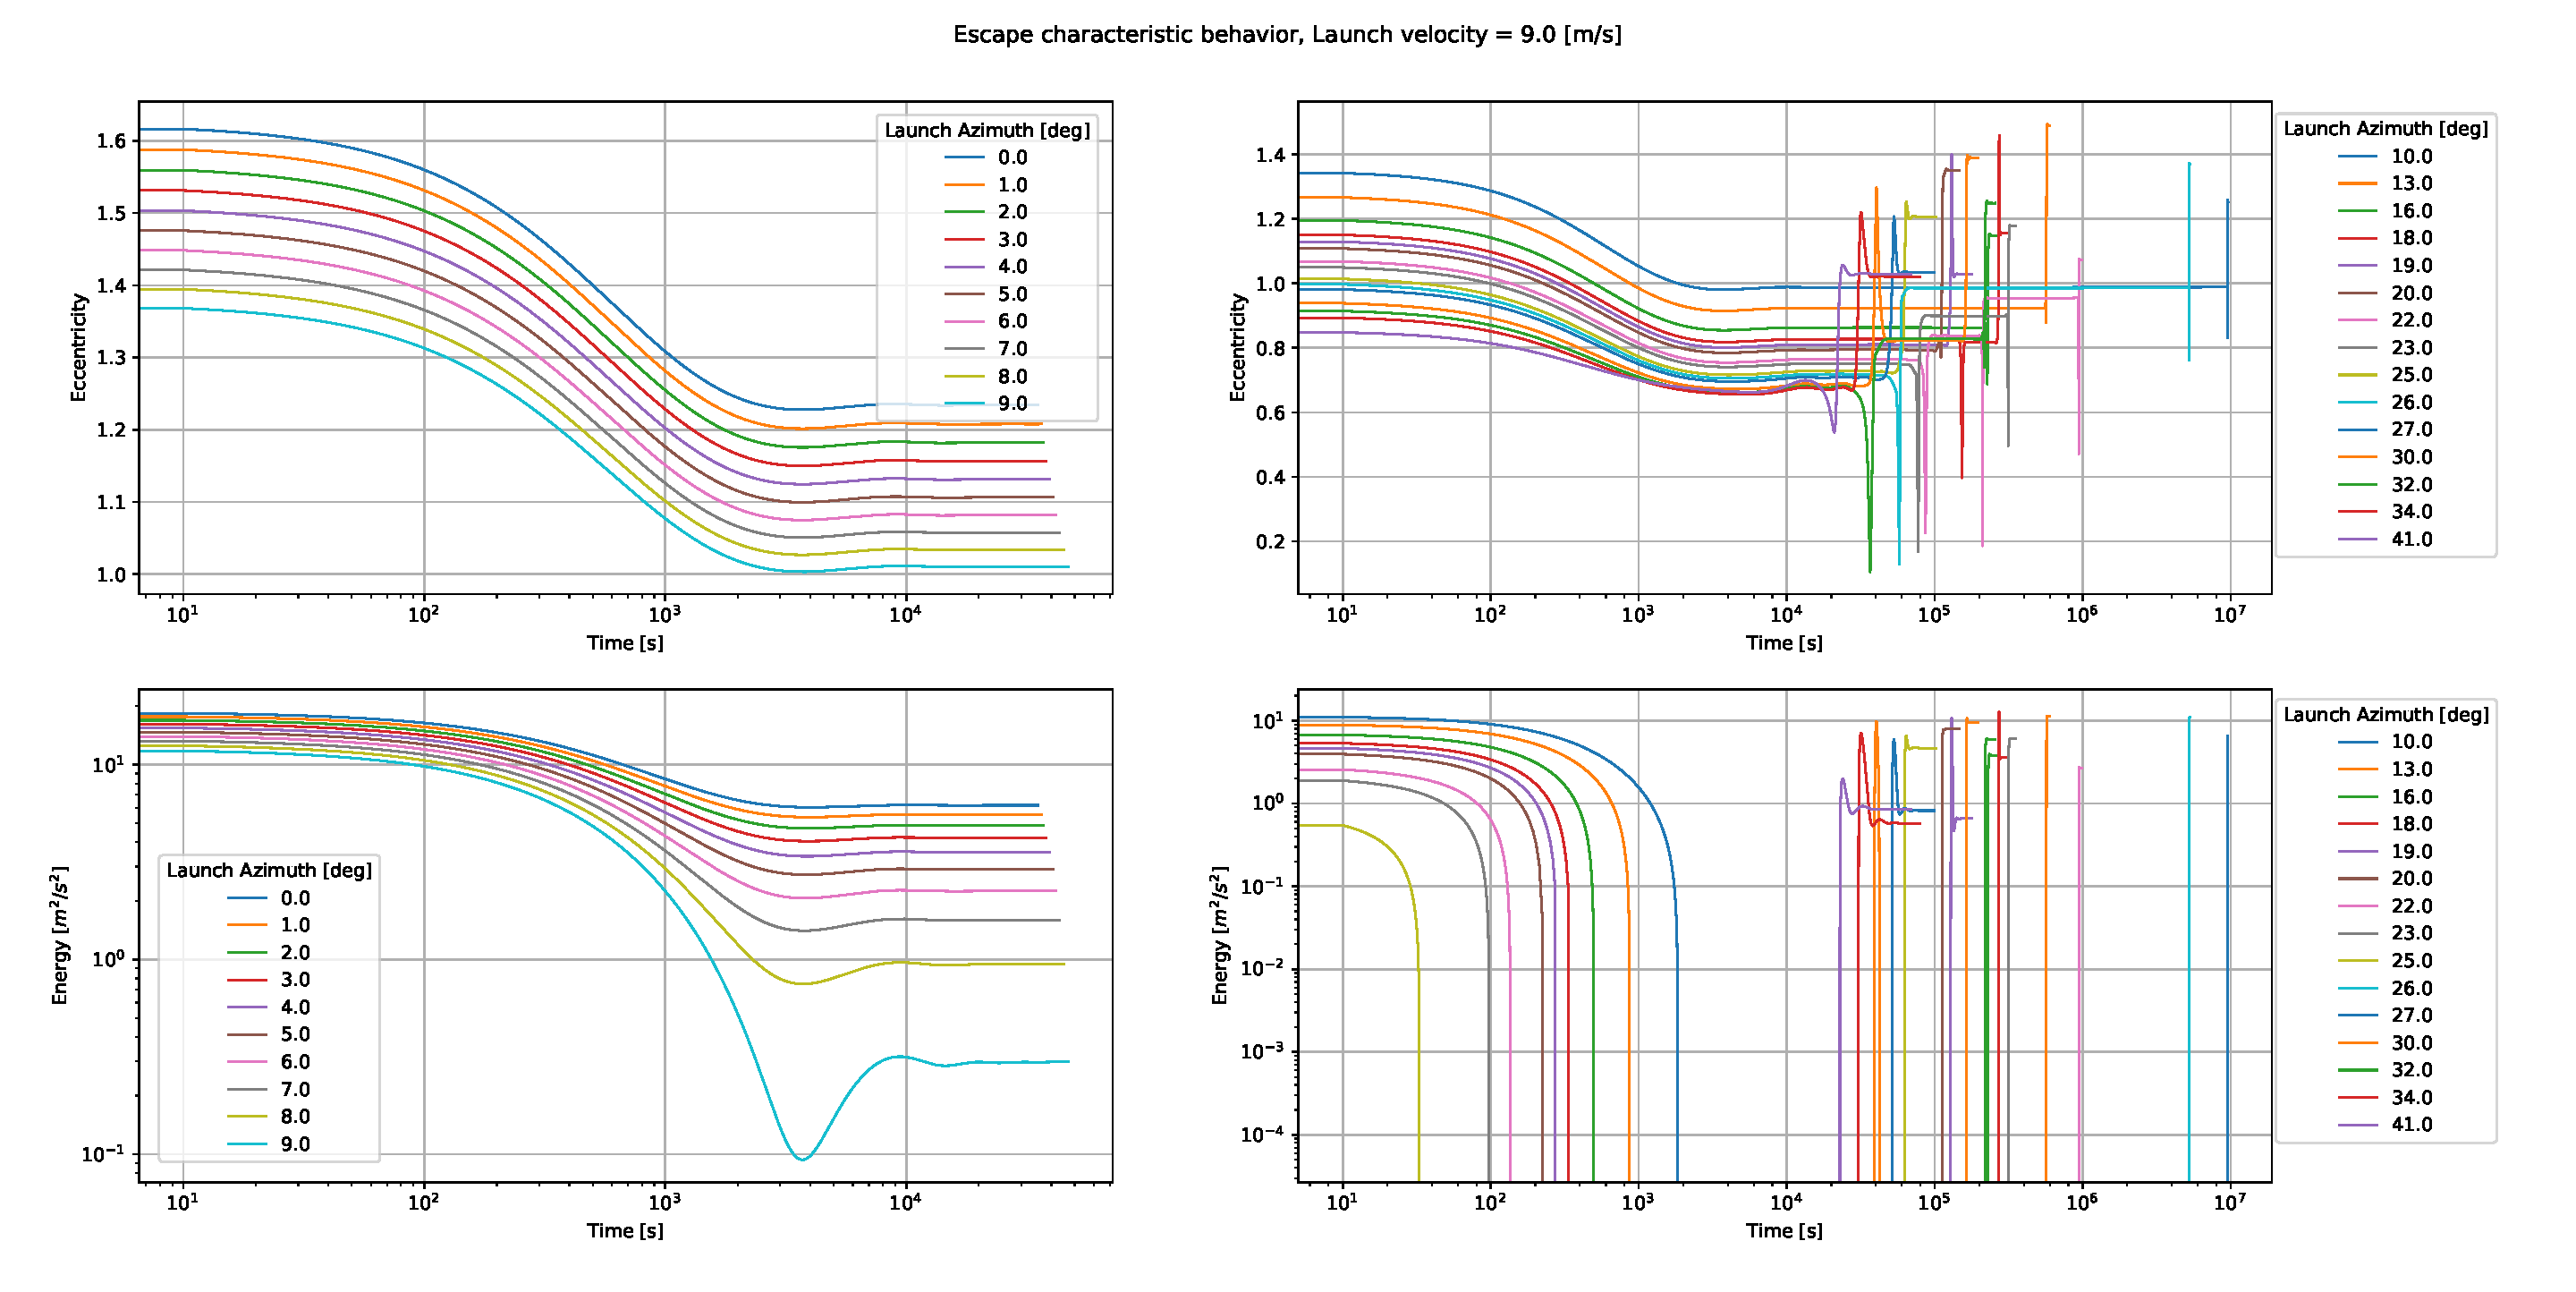
\includegraphics[angle=90, width=\textwidth, height=\textheight, keepaspectratio=true]{Images/longest_edge_no_perturbations/escape_energy_ecc_9ms.pdf}
\caption{Osculating energy and eccentricity for all escape cases as shown in \protect\Cref{fig:hev_9ms_lowerAzimuths_noSP}. The energy plot is shown in an unorthodox way by using a logarithmic scale to easily distinguish energies that stay positive for the entire duration until escape. If the energy becomes negative, then on this scale, the corresponding curve appears to be going straight downwards in the plot (since a negative value is not defined on the log scale). Similarly, if the energy becomes positive from a negative value earlier, then the curve appears to be coming upwards straight (again from some hypothetical negative value at the bottom of the log scale).}
\label{fig:energy_ecc_escape_9ms_noSP}
\end{figure}
\FloatBarrier
%%%
From the previous observation, we can also confirm the pattern of variation in the \gls{HEV} values for non-chaotic data points in \Cref{fig:hev_escapeHist_noSP}. If we consider looking at the \SI{13}{\metre\per\second} case, as an example, we see that the \gls{HEV} increases with increasing launch azimuth values beyond \SI{100}{\degree} up until \SI{270}{\degree}. This happens because for increasing launch azimuths in this range, the particle's inertial launch velocity increases as well as the azimuths align more and more in the asteroid's rotational direction and becomes maximum for the exact azimuth of \SI{270}{\degree}. Now we saw earlier that these particles are inherently on an escape trajectory immediately after launch and don't require gravity assists from the rotating asteroid to be on one. This implies that if the inertial launch velocity itself is high, then the inertial velocity at the instance of escape remains high too, which is what we observe in the plots.

% \subsection{Final Fate Predetermination}
% \label{subsec:final_fate_predetermine_noSP}
% From all the results that we have seen so far, we get a hint that it is not easy to distinguish between escape and re-impact\footnote{Capture case wasn't witnessed for the simulation type being discussed in this chapter}. The boundary between them is blurred. In this section, we'll look at the initial values for the osculating semi-major axis and eccentricity to see if final fate can be distinguished based on the shape of the initial osculating orbit. Then we take a look at the initial values for the osculating inclination, \gls{RAAN}, and \gls{AOP} to see if final fates can be distinguished based on the orientation of the initial osculating orbit. We also look at the progression of the eccentricity and inclination vector to see if there is a distinct demarcation between the re-impact and escape cases. Results are presented only for particles launched with a velocity of \SI{8}{\metre\per\second} and in all azimuth directions. This is done to ensure the plots don't get overcrowded with data points from all launch velocities and also because a single launch velocity was sufficient to represent the relevant information.
% %%%
% \begin{figure}[htb]
% \centering
% \captionsetup{justification=centering}
% \includegraphics[angle=90, width=\textwidth, height=\textheight, keepaspectratio=true]{Images/longest_edge_no_perturbations/initial_orbital_elements_8ms_edited.pdf}
% \caption{Initial values of the osculating orbital elements for regolith launched with a velocity of \SI{8}{\metre\per\second} and in all azimuth directions.}
% \label{fig:init_orbitalElements_8ms_noSP}
% \end{figure}
% \FloatBarrier
% %%%

\subsection{Sensitivity To Launch Conditions}
\label{subsec:sensitivity_noSP}
In this section, we will briefly highlight how regolith motion is sensitive in terms of their final fate, i.e., escape or re-impact. If you recall from \Cref{sec:simulation_setup_noSP}, the launch site and launch declination angle remain constant in this simulation exercise. We vary only the launch azimuth angle and the launch velocity of the regolith while lofting them. Hence, we judge the sensitivity in terms of these two initial elements.
%
\newline\newline
%
\Cref{fig:270Azim_traj_noSP} highlights the difference between two trajectories that were launched with the same azimuth angle but differently launch velocities. An escape situation is encountered when the particle is launched with a velocity of \SI{4}{\metre\per\second} while the same particle re-impacts when launched with a velocity of \SI{5}{\metre\per\second}. With the resolution of launch conditions established in general for our simulation, and for every other launch condition being the same, the particle is sensitive to either of the final fates with \SI{1}{\metre\per\second} of a difference in the launch velocity.
%
\newline\newline
%
\Cref{fig:10ms_traj_noSP} highlights the difference between two trajectories when the launch velocity is the same, i.e. \SI{10}{\metre\per\second}, but the launch azimuths are different. So at azimuth \SI{41}{\degree}, the particle escapes while at \SI{42}{\degree} the particle re-impacts the asteroid. Thus, for all other launch conditions being the same, the particle is sensitive to either of the final fates to a \SI{1}{\degree} launch azimuth resolution.
%
\newline\newline
%
The current discussion, albeit short, was to see if the sensitivity (in terms of final fate acquired by regolith) had a magnitude equal to the resolution of varying the launch conditions in the current simulation scenario. This was found to be true, but, from all the results that we have seen so far and looking at how blurry the line in distinguishing the two fates, a similar sensitivity behavior can be expected if the resolution of launch conditions is lowered.

% \section{Conclusions}
% \label{sec:conclusions_noSP}

%%%
\begin{figure}[htb]
\centering
\captionsetup{justification=centering}
\subfloat[]{
    \includegraphics[width=\textwidth, height=0.5\textheight, keepaspectratio=true]{Images/longest_edge_no_perturbations/4ms_270Azim_escape.pdf}
    \label{fig:4ms_270Azim_traj_noSP}
}

\subfloat[]{
    \includegraphics[width=\textwidth, height=0.5\textheight, keepaspectratio=true]{Images/longest_edge_no_perturbations/5ms_270Azim_reimpact.pdf}
    \label{fig:5ms_270Azim_traj_noSP}
}
\caption{Regolith trajectory, expressed in the \gls{AIF}, for particles launched with azimuth \SI{270}{\degree} and velocity of \protect\subref{fig:4ms_270Azim_traj_noSP} \SI{4}{\metre\per\second} and \protect\subref{fig:5ms_270Azim_traj_noSP} \SI{5}{\metre\per\second}.}
\label{fig:270Azim_traj_noSP}
\end{figure}
\FloatBarrier
%%%
%%%
\begin{figure}[htb]
\centering
\captionsetup{justification=centering}
\subfloat[]{
    \includegraphics[width=\textwidth, height=0.5\textheight, keepaspectratio=true]{Images/longest_edge_no_perturbations/10ms_41Azim_escape.pdf}
    \label{fig:10ms_41Azim_traj_noSP}
}

\subfloat[]{
    \includegraphics[width=\textwidth, height=0.5\textheight, keepaspectratio=true]{Images/longest_edge_no_perturbations/10ms_42Azim_reimpact.pdf}
    \label{fig:10ms_42Azim_traj_noSP}
}
\caption{Regolith trajectory, expressed in the \gls{AIF}, for particles launched with velocity \SI{10}{\metre\per\second} and azimuth of \protect\subref{fig:10ms_41Azim_traj_noSP} \SI{41}{\degree} and \protect\subref{fig:10ms_42Azim_traj_noSP} \SI{42}{\degree}.}
\label{fig:10ms_traj_noSP}
\end{figure}
\FloatBarrier
%%%

\chapter{Dynamics With Solar Perturbations}
\label{chap:dynamics_with_solar_perturbations}
\graphicspath{{Results/Images/}}

The discussion on results so far have not accounted for any Solar perturbations in the simulations. In this chapter, however, we will see how adding \gls{STBE} and \gls{SRP} perturbing accelerations, in addition to the non-uniform gravity field of the asteroid, affects the motion of regolith and if any capture orbits are obtained due to them.

\section{Regolith Size and Density}
\label{sec:regolith_size_density}
Before we can present the results of any simulation, we need to justify the size and density of different regolith types used. We used two different density values and two different grain radii and thereby used four different area-to-mass ratios. The selection of regolith types was made by using asteroid Eros as an example. The different area-to-mass ratios are mentioned in \Cref{tab:area_to_mass_ratio}.

\subsection{Density Selection}
\label{subsec:regolith_density_selection}
The material with a density of 3.2 g/cm$^3$ is low-density Olivine (Magnesium Iron Silicates) and the one with 7.5 g/cm$^3$ is Iron-Nickel alloy \parencite{passiveSorting}. We have chosen these two types of materials based on the surface composition analysis of asteroid Eros, an S-Type asteroid, from the \gls{NEAR}-Shoemaker data. S-Type asteroids, from reflectance spectral analysis, are commonly known to have minerals like Olivine, Pyroxene, and Fe-Ni (Iron-Nickel) metal \parencite{Nittler2001}. Thermo-spectral analysis of regolith on Eros reveals that it is rich in Olivine and is found to be more abundant than Pyroxene \parencite{McCoy2001}. The mineral Olivine has also been discovered on Itokawa, another S-Type asteroid, through transmission electron microscope analysis of samples returned by the Hayabusa spacecraft \parencite{olivineHayabusa}.
%
\newline\newline
%
Eros also contains Fe-Ni but it is significantly separated from the Silicates (Olivine and Pyroxene) within the regolith \parencite{Nittler2001}. \cite{Evans2001} analyzed elemental composition of \gls{NEAR}-Shoemaker's landing site on Eros, based on which, it presents several arguments for relatively lower abundance of Fe (Iron) on the surface of Eros. One of the arguments hypothesizes that different grain sizes and density of Fe-Ni from Olivine could have resulted in the metal to get separated from the Silicates, either spatially or for it to sink down in the lower depths of the regolith. In light of this, we are considering regolith comprising of only Olivine and Fe-Ni, to distinguish between their orbital behavior and final fate upon being lofted from the surface of an asteroid such as Eros.

\subsection{Size Selection}
\label{subsec:regolith_size_selection}
\cite{Veverka2001} analyzed high-resolution surface images of Eros captured by \gls{NEAR}-Shoemaker on a low-altitude flyover. It argued the build-up of a heterogeneous and complex regolith that comprised of material ranging from fine particles all the way up to metre-sized ejecta blocks. \cite{Veverka2001} argues that while there is an abundance of large ejecta blocks across the surface, the much finer regolith occupies mostly the low-lying topographies, i.e., inside large craters on the surface of Eros. The latter was termed as ponded deposits. \cite{Robinson2001} argues, from high-resolution images (1.2 cm per pixel) of ponded deposits at Eros, that the grain size of regolith would be around 1.0 cm or below.
%
\newline\newline
%
Thus based on this extreme spectra of regolith composition at Eros, we shall also consider regoliths with varying densities and grain radii (each grain is assumed to be spherical). These are listed in \Cref{tab:area_to_mass_ratio}. The particles are listed in decreasing order of area-to-mass ratio.
% We considered coarse regolith of 10 [cm] radius as well, the motivation for which comes from the size of the ejecta blocks generated from the impact of \gls{NEAR}-Shoemaker on Eros's surface. \cite{Robinson2001} notes that their are several 10 [cm] ejecta blocks around the \gls{NEAR}-Shoemaker impact site. Thus, ejecta size of 10 [cm] in radii is justified for this study in the context of an asteroid exploration or exploitation mission.
%%%
\begin{table}[htb]
\centering
\captionsetup{justification=centering}
\caption{Particle area-to-mass ratios}
\label{tab:area_to_mass_ratio}
\begin{tabular}{|l|c|c|c|}
\hline
Code    & \multicolumn{1}{l|}{Particle radius {[}cm{]}} & \multicolumn{1}{l|}{Density {[}g/cm$^3${]}} & \multicolumn{1}{l|}{area-to-mass ratio {[}m$^2$/kg{]}} \\ \hline
LoGSP-1     &   1.0     &   3.2     & 0.0234        \\ \hline
LoGSP-2     &   1.0     &   7.5     & 0.01          \\ \hline
LoGSP-3     &   5.0     &   3.2     & 0.0047        \\ \hline
LoGSP-4     &   5.0     &   7.5     & 0.002         \\ \hline
% LoGSP-5     &   10.0    &   3.2     & 0.0023        \\ \hline
% LoGSP-6     &   10.0    &   7.5     & 0.001         \\ \hline
\end{tabular}
\end{table}
\FloatBarrier
%%%

\section{Simulation Setup}
\label{sec:simulation_setup}
The initial conditions for lofting each type of regolith are varied in the same manner and are mentioned as follows. The asteroid revolves around the Sun in an equatorial circular orbit at a distance of 1.0 AU. Four different initial Solar phase angles were considered for the simulation (\SI{45.0}{\degree}, \SI{135.0}{\degree}, \SI{225.0}{\degree} \SI{315.0}{\degree}), to account for the four different quadrants where the Sun could be with respect to the asteroid.
%
\newline\newline
%
For each case in \Cref{tab:area_to_mass_ratio}, a total of 72 particles\footnote{Recall that in the previous chapter, the number of particles were launched at an azimuth resolution of \SI{1}{\degree} which resulted in 360 particles being launched} were launched from the surface of the asteroid, each in a different direction. The launch declination angle was kept constant at \SI{45.0}{\degree}  for all particles. The launch azimuth was varied at a resolution of \SI{5.0}{\degree}  starting from \SI{0.0}{\degree}  all the way up to \SI{355.0}{\degree} . Each particle was launched, in their specified direction, with different velocities ranging from 1.0 to \SI{16.0}{\metre\per\second} (measured with respect to the \gls{ARF}) at a resolution of \SI{1.0}{\metre\per\second}. So basically, every combination of an initial Solar phase angle, initial launch azimuth, and initial launch velocity corresponds to a unique trajectory for a single particle of a given area-to-mass ratio; thus amounting to a total of 4608 unique trajectories for each regolith type.
%
\newline\newline
%
We choose three different launch sites this time; the first being the longest edge of the \gls{CDE} at latitude and longitude both \SI{0}{\degree}; the second being the leading edge at latitude and longitude both \SI{45}{\degree}; and finally the third being the trailing edge of the asteroid at latitude \SI{45}{\degree} and longitude \SI{-45}{\degree}. However, for a detailed analysis on the effects of Solar perturbations on regolith motion (discussed in \Cref{sec:LoGSP-1}), we will consider only the longest edge launch site. The remaining launch sites will be used later on to present more general and statistical results (\Cref{sec:final_fate_general_all_launch_sites}) that characterize the final fate and orbital motion of regolith based simply on different grain size and density, for the respective launch sites.

\section{Solar Perturbation Analysis}
\label{sec:LoGSP-1}
We now present the orbital motion analysis for one of the regolith types, particle LoGSP-1, when lofted from the longest edge of the asteroid. We choose this particular regolith type since it offers the maximum area-to-mass ratio. A larger value for area-to-mass ratio means a relatively larger effect of \gls{SRP} on the regolith which makes it more interesting since for a detailed analysis we want to see how \gls{SRP} (as well as \gls{STBE} in general) affects the orbital motion of regolith. Presenting a similar detailed analysis for all particle types will not be practical for the purposes of this report since it will become repetative.

\subsection{Comparison With Unperturbed Scenario}
\label{subsec:noSP_comparison_reimpact_and_escape}
We will begin with a very brief comparison of the final fate characteristics of regolith from when the Solar perturbations were included in our simulation, with the case when they were excluded. Note that, when we say unperturbed, it simply means the exclusion of the \gls{SRP} and \gls{STBE} and not the non-uniform gravity field. Since the only two outcomes in the unperturbed scenario were escape and re-impact, we compare them with the results from the simulation with perturbations.
%
\newline\newline
%
We begin by first comparing the re-impact behavior. \Cref{fig:three_velocity_crashmap_comparison_noSP} shows the re-impact locations for regolith launch in an environment with no Solar perturbations, with three different launch velocities as shown in the plot. The plot is the same as \Cref{fig:crashmap_launchAzimuth_noSP} except that the launch azimuth resolution is \SI{5}{\degree} instead of \SI{1}{\degree}. Similarly, \Cref{fig:three_velocity_crashmap_comparison_sp} shows the re-impact locations for regolith simulated with Solar perturbations. The two cases are very similar to each other. The location and shape of the re-impact points, forming an arc on the West of the launch site for launch velocities of 5 and \SI{9}{\metre\per\second}, remains the same for both the perturbed and unperturbed scenario. In those cases, the trajectories are short lived and ballistic and the perturbations do not get enough time to accumulate and change the trajectory. For all other re-impact points, the numbers are smaller for the perturbed case and the corresponding re-impact locations are different from the unperturbed counterpart. In general, the re-impact map for the perturbed scenario shares a good resemblance with the unperturbed one. This aforementioned features of the re-impact locations was found to be similar for results from all four initial Solar phase angles considered in the simulations, but the plots for each are not shown in this report for brevity.
%
\newline\newline
%
Now we will look at the escape behavior. The correlation between escape trajectories and distribution of data points in the \gls{HEV} versus launch azimuth plot, discussed in \Cref{subsec:escape_behavior_noSP}, was found to be true even in the case of the perturbed simulation. We show an example case for launch velocity of \SI{9}{\metre\per\second} and for launch azimuths from \SI{0}{\degree} to \SI{20}{\degree} in steps of \SI{1}{\degree}, in \Cref{fig:escape_9ms_noSP_spanalysis}. What we see in the figure is that for all launch azimuths below \SI{10}{\degree}, the particles are on an escape trajectory immediately after launch. For escaping particles with launch azimuth above \SI{10}{\degree}, the particles required gravity assists from the asteroid and involved taking one or more revolutions around it before finally escaping.
%
\newline\newline
%
So far the behavior and the explanation for it is the same as that in \Cref{subsec:escape_behavior_noSP}, however, there is a critical case witnessed here at launch azimuth \SI{10}{\degree}. From the discussion earlier and from \Cref{fig:escape_hev_9ms_phase45}, one would say that this particle should already be on an escape trajectory as it is aligned with the smoothly reducing \gls{HEV} data points of lower azimuths. But that is not the case. Also note that the \gls{HEV} for it is \SI{0}{\metre\per\second} and from \Cref{fig:escape_energy_ecc_9ms_phase45} we see that at the time of escape the trajectory has an eccentricity of 1.0. Both these facts confirm that the osculating trajectory finally becomes parabolic at the instance of escape. This is perhaps why this particular regolith does not share the same traits with any other launch azimuth, because in every other case the escape trajectory is hyperbolic.
%%%
\begin{figure}[htb]
\centering
\captionsetup{justification=centering}
\subfloat[]{
    \includegraphics[angle=90, width=\textwidth, height=0.5\textheight, keepaspectratio=true]{longest_edge_perturbations/3.2Density_1cmSize/compare_with_noSP/three_velocity_crash_map_noSP.pdf}
    \label{fig:three_velocity_crashmap_comparison_noSP}
}

\subfloat[]{
    \includegraphics[angle=90, width=\textwidth, height=0.5\textheight, keepaspectratio=true]{longest_edge_perturbations/3.2Density_1cmSize/compare_with_noSP/three_velocity_crash_map_phase45.pdf}
    \label{fig:three_velocity_crashmap_comparison_sp}
}
\caption{Re-impact locations for three specific velocities, where for each velocity, the launch azimuth varies with a resolution of \SI{5}{\degree}. Out of the two figures, \protect\subref{fig:three_velocity_crashmap_comparison_noSP} shows the results for the unperturbed scenario and \protect\subref{fig:three_velocity_crashmap_comparison_sp} shows the results for the case with the perturbations. For the latter, the initial Solar phase angle is \SI{45}{\degree} and particle code is LoGSP-1.}
\label{fig:specific_velocity_crashMap_noSP_spanalysis}
\end{figure}
\FloatBarrier
%%%
%%%
\begin{figure}[htb]
\centering
\captionsetup{justification=centering}
\subfloat[]{
    \includegraphics[angle=90, width=\textwidth, height=0.4\textheight, keepaspectratio=true]{longest_edge_perturbations/3.2Density_1cmSize/compare_with_noSP/escape_hev_9ms_phase45_1degAzimResolution.pdf}
    \label{fig:escape_hev_9ms_phase45}
}

\subfloat[]{
    \includegraphics[angle=90, width=\textwidth, height=0.5\textheight, keepaspectratio=true]{longest_edge_perturbations/3.2Density_1cmSize/compare_with_noSP/escape_energy_ecc_9ms_phase45_1degAzimResolution.pdf}
    \label{fig:escape_energy_ecc_9ms_phase45}
}
\caption{Escape behavior for regolith launched with a velocity of \SI{9}{\metre\per\second}; launch azimuths shown here range from \SI{0}{\degree} to \SI{20}{\degree} in steps of \SI{1}{\degree}, which is sufficient to discuss the topic at hand. Out of the two figures, \protect\subref{fig:escape_hev_9ms_phase45} shows the \gls{HEV} data points and \protect\subref{fig:three_velocity_crashmap_comparison_sp} shows the energy and eccentricity curves for the corresponding cases. For the latter, the initial Solar phase angle is \SI{45}{\degree} and particle code is LoGSP-1.}
\label{fig:escape_9ms_noSP_spanalysis}
\end{figure}
\FloatBarrier
%%%

\subsection{Final Fate General Characteristics}
\label{subsec:final_fate_charac_general}
\Cref{fig:LoGSP_1_final_fate_histogram} gives a distribution of particles for each of the three different final fates for the regolith i.e. capture, re-impact, and escape, for different initial launch velocities and initial Solar phase angles. Irrespective of the initial Solar phase, initial launch velocities from 1.0 to \SI{3.0}{\metre\per\second} results in particles launched in all directions to eventually re-impact the asteroid's surface. Similarly, for initial launch velocities ranging from 14 to \SI{16.0}{\metre\per\second}, we see that the particles always manage to escape the gravitational attraction of the asteroid\footnote{There is one exception though, at \SI{14.0}{\metre\per\second} and for launch azimuth of \SI{90}{\degree} and Solar phase angle of \SI{315}{\degree}, the particle re-impacts}. Launch velocities from 4 to \SI{13.0}{\metre\per\second} show a mixed behavior and the final fate distribution trend does not vary drastically for different initial Solar phase angles. Looking at absolute numbers, for all Solar phase angles combined, about 54.9\% cases result in an escape situation, 44.8\% cases result in re-impact and a mere 0.2\% cases result in a capture scenario. Thus, the number of capture cases is extremely small relative to the other two final fates.
%
\newline\newline
%
For initial Solar phase of \SI{225.0}{\degree}, there are no cases of regolith being captured in orbit around the asteroid. All capture cases, arranged in order of increasing launch azimuth angle, are listed in \Cref{tab:LoGSP_1_capture}. It is interesting to note that all capture cases result from when the particle is launched in a direction which is against the direction of rotation of the asteroid.
%%%
\begin{table}[htb]
\centering
\captionsetup{justification=centering}
\caption{Initial conditions that resulted in temporary orbital capture of regolith around the asteroid. Particle code LoGSP-1.}
\label{tab:LoGSP_1_capture}
\begin{tabular}{|l|c|c|c|}
\hline
Index & \multicolumn{1}{l|}{Launch azimuth [deg]} & \multicolumn{1}{l|}{Launch velocity [m/s]} & \multicolumn{1}{l|}{Initial Solar phase angle [deg]} \\ \hline
\rowcolor[HTML]{FE996B}
1   & 5.0 & 5.0 & 315.0     \\ \hline
\rowcolor[HTML]{67FD9A}
2   & 10.0 & 9.0 & 135.0    \\ \hline
\rowcolor[HTML]{9698ED}
3   & 15.0 & 8.0 & 45.0     \\ \hline
\rowcolor[HTML]{FFCC67}
4   & 45.0 & 12.0 & 45.0    \\ \hline
\rowcolor[HTML]{96FFFB}
5   & 45.0 & 10.0 & 315.0   \\ \hline
\rowcolor[HTML]{FFCC67}
6   & 135.0 & 12.0 & 45.0   \\ \hline
\rowcolor[HTML]{96FFFB}
7   & 135.0 & 10.0 & 315.0  \\ \hline
\rowcolor[HTML]{9698ED}
8   & 165.0 & 8.0 & 45.0    \\ \hline
\rowcolor[HTML]{67FD9A}
9   & 170.0 & 9.0 & 135.0   \\ \hline
\rowcolor[HTML]{FE996B}
10  & 175.0 & 5.0 & 315.0   \\ \hline
% 11  & 185.0 & 5.0 & 135.0   \\ \hline
\end{tabular}
\end{table}
\FloatBarrier
%%%
The capture cases which represent symmetry in terms of the launch azimuth angle are highlighted with the same color in \Cref{tab:LoGSP_1_capture}. This symmetric behavior results from the combination of two factors. First, the Sun's motion relative to the asteroid is not in an inclined plane, and secondly, the particles are launched from the equatorial tip of the ellipsoid shaped asteroid, which is a point of symmetry on the ellipsoid. The capture cases are discussed in detail in \Cref{subsec:capture_orbit_analysis_as_is}.
%
\newline\newline
%
\Cref{fig:LoGSP_1_crashmap} depicts the surface distribution of regolith that re-impacts the surface when launched from the same location with different velocities and different initial Solar phase angles. The launch location is in the centre of the map, latitude and longitude \SI{0.0}{\degree}.
%%%
\begin{figure}[htb]
\centering
\captionsetup{justification=centering}
\includegraphics[angle=90, width=\textwidth, height=\textheight, keepaspectratio=true]{longest_edge_perturbations/3.2Density_1cmSize/final_fate_versus_launch_velocity_histogram_all_solar_phases.pdf}
\caption{Histogram showing the number of particles that re-impact, escape, or get captured around the asteroid, for different initial launch velocities. Particle code LoGSP-1.}
\label{fig:LoGSP_1_final_fate_histogram}
\end{figure}
\FloatBarrier
%%%
The re-impact locations remains unchanged, irrespective of the initial Solar phase angles, for all particles launched with the relatively lower velocities (1 to \SI{4}{\metre\per\second}). Again for the mid-range velocities, i.e. 5 to \SI{9}{\metre\per\second}, the re-impact locations for the particles that are launched in the direction opposite to the asteroid's rotation remains unchanged for different initial Solar phase angles. This can be observed in the arc shaped re-impact location patterns West of the launch location for those velocities. The distribution pattern, for all launch velocities and initial Solar phases, is also symmetric about the equator. Again, the reason for this is the same as mentioned earlier for the symmetry in capture cases in \Cref{tab:LoGSP_1_capture}. In general, keeping the launch direction and velocity constant, we see that the distribution of re-impact locations does not change drastically with varying initial Solar phase angles. This is much easily observed in a plot of the range from the launch site to the re-impact point versus launch azimuth for different velocities as shown in \Cref{fig:LoGSP_1_range_comparison}.
% %
% \newline\newline
% %
% We have not shown the range to re-impact point plots in \Cref{fig:LoGSP_1_range_comparison} for all launch velocities because the intention here is to show the qualitative behavior, which can be achieved by considering only a subset of the launch velocities that result in a re-impact scenario. The very first thing we observe is that as the launch velocity increases, the range of launch azimuth over which the regolith re-impacts the surface reduces because a higher velocity allows the regolith to enter a higher orbit (as it attains a relatively higher energy) and reduces the probability of a re-impact. Even as the velocity increases, we see that the azimuths that result in a re-impact are the ones in which the regolith is launched in a direction that is opposite to the asteroid's rotation direction. This makes sense since the regolith's energy would be reduced the most in this scenario compared to all other launch directions, thereby increasing the chances of a re-impact.
% %
% \newline\newline
% %
% Now the primary purpose of the plots in \Cref{fig:LoGSP_1_range_comparison} (combined with \Cref{fig:LoGSP_1_crashmap}) is to depict the qualitative effect of Solar perturbations, for varying initial Solar phase angles, on the re-impact behavior of regolith compared to the case when no Solar perturbations are considered. For launch velocities of 4.0, 7.0 and \SI{10.0}{\metre\per\second}, we see that the Solar perturbations do not affect the re-impact location for cases when the particle is launched in directions opposite to that of the asteroid's rotation. However, we do see few exceptions to the former statement, most noticeably in the case of \SI{7.0}{\metre\per\second}. But for the majority of cases where the re-impact location remains unchanged, we see from \Cref{fig:LoGSP_1_reimpact_time}, that these particles spend less than 3.0 hours in orbit which is not enough time for the Solar perturbations to act and have any significant impact on the dynamics of the particles. So in essence this is what is happening here - particles when launched in a direction that is opposite to that of the asteroid's rotation, even at relatively high velocities such as \SI{10.0}{\metre\per\second}, loose enough energy to stay in a relatively lower orbit (see \Cref{fig:LoGSP_1_maxAltitude_reimpactscenario}) where the gravitational force of the asteroid is significantly stronger than any of the Solar perturbations and as the particle spends a very short time in orbit before re-impact, the Solar perturbations do not get enough time to affect the particle's orbit and hence the particle re-impacts the same location as it would have when no Solar perturbations were considered in the simulation. For the lower launch velocities of 4.0 and \SI{7.0}{\metre\per\second}, the differences in re-impact locations are more pronounced when the regolith is launched in the same direction as that of the asteroid's rotation. Particles gain relatively higher energy in this case, enter a higher orbit and spend enough time there for the Solar perturbations to affect its motion. For the case of the launch velocity of \SI{13.0}{\metre\per\second} in \Cref{fig:LoGSP_1_range_comparison}, the velocity is high enough such that the particle does not loose enough energy when launched opposite to the asteroid's rotational direction and is able to enter a relatively higher orbit (see \Cref{fig:LoGSP_1_maxAltitude_reimpactscenario}) and stay there for a relatively longer time, as seen in \Cref{fig:LoGSP_1_reimpact_time}, which results in the Solar perturbations affecting the orbital motion and eventually the re-impact location of the regolith.
%%%
\begin{figure}[htb]
\centering
\captionsetup{justification=centering}
\includegraphics[angle=90, width=\textwidth, height=\textheight, keepaspectratio=true]{longest_edge_perturbations/3.2Density_1cmSize/crash_map_all_solar_phases.pdf}
\caption{Surface distribution of re-impacted regolith for different launch velocities. The launch location is \\ latitude: \SI{0}{\degree}, longitude: \SI{0.0}{\degree}. Particle code LoGSP-1.}
\label{fig:LoGSP_1_crashmap}
\end{figure}
\FloatBarrier
%%%

\subsection{Capture Orbit Analysis}
\label{subsec:capture_orbit_analysis_as_is}
We shall now look at the cases where the lofted regolith gets (temporarily) captured in orbit by the asteroid. The initial conditions for all capture cases, for the current particle size and density, were mentioned earlier in \Cref{tab:LoGSP_1_capture}. \Cref{fig:LoGSP_1_capture_orbital_range} depicts the progression in orbital range of the temporarily captured regolith. The straight lines in the plot are used to mark the different altitude regimes. These are the \gls{LAO}, \gls{MAO}, \gls{HAO}, \gls{UHAO}, and \gls{EHAO}. These altitude regime definitions are not from well defined standards, but instead were arbitrarily chosen as integer multiples of the longest semi-axis, $\alpha$, of the tri-axial ellipsoid shaped asteroid. The definition for these altitude regimes is given in \Cref{tab:altitude_regimes}.
%%%
\begin{table}[htb]
\centering
\captionsetup{justification=centering}
\caption{Altitude regimes and their definitions}
\label{tab:altitude_regimes}
\begin{tabular}{|c|c|}
\hline
\textbf{Altitude regime}        & \textbf{Definition}                    \\ \hline
\gls{LAO}                       & Asteroid surface to $2 \times \alpha$  \\ \hline
\gls{MAO}                       & $2 \times \alpha$ to $3 \times \alpha$ \\ \hline
\gls{HAO}                       & $3 \times \alpha$ to $5 \times \alpha$ \\ \hline
\gls{UHAO}                      & $5 \times \alpha$ to $7 \times \alpha$ \\ \hline
\gls{EHAO}                      & Above $7 \times \alpha$                \\ \hline
\end{tabular}
\end{table}
\FloatBarrier
%%%
The purpose of plotting data as shown in \Cref{fig:LoGSP_1_capture_orbital_range} was to look for any patterns or periodicity, if they existed, and to see if particles in temporary capture scenario remain closer to the asteroid or further away from it. The symmetry as explained for initial conditions mentioned in \Cref{tab:LoGSP_1_capture} can also be seen in \Cref{fig:LoGSP_1_capture_orbital_range}, for example, regolith launched with velocity of \SI{8.0}{\metre\per\second} and launch azimuth of \SI{15.0}{\degree} (shown by the purple curve in the top plot in \Cref{fig:LoGSP_1_capture_orbital_range}) shows the same behavior as that of regolith launched with the same velocity and \SI{165.0}{\degree} launch azimuth (shown by the green curve in the bottom plot in \Cref{fig:LoGSP_1_capture_orbital_range}). Another thing we see from the plot is that the captured regolith stay in the higher altitude regions for most part and only briefly do they fall within the \gls{MAO} and \gls{LAO} region. We shall now take a look at a few cases from \Cref{fig:LoGSP_1_capture_orbital_range} in a bit more detail to understand the effect of Solar perturbations by comparing these cases with their unperturbed counterparts.
%
\newline\newline
%
Of all the cases shown in \Cref{fig:LoGSP_1_capture_orbital_range} or \Cref{tab:LoGSP_1_capture}, the one with a launch velocity of \SI{10.0}{\metre\per\second} and launch azimuth of \SI{45.0}{\degree} results in a re-impact scenario when Solar perturbations are omitted, but the same initial conditions lead to a temporary capture orbit when perturbations were added for an initial Solar phase angle of \SI{315.0}{\degree}. Every other initial condition for the capture cases had otherwise resulted in an escape situation when simulations were conducted without the Solar perturbations. The 3D trajectory plot in two different views for the former case are shown in \Cref{fig:LoGSP_1_capture_case_5_3d_traj_inertialFrame_differnetViews} (see \Cref{fig:LoGSP_1_capture_case_5_3d_trajectory} also for the 3D trajectory representation in the \gls{ARF}). The 2D trajectory for the same is shown in \Cref{fig:LoGSP_1_capture_case_5_2d_traj_inertialFrame} in inertial frame and in \Cref{fig:LoGSP_1_capture_case_5_2d_traj_bodyFrame} in the \gls{ARF} or the body frame. The web-link or URL for the trajectory animation of the particle (in inertial frame and in XY-plane only) can be found in \Cref{fig:LoGSP_1_capture_case_5_2d_trajectory_animation}.
%%%
\begin{figure}[htb]
\centering
\captionsetup{justification=centering}
\includegraphics[scale=0.2]{longest_edge_perturbations/3.2Density_1cmSize/qrcode_10ms_45Azimuth_315SolarPhase.png}
\caption{2D trajectory animation (XY-Plane) of capture regolith for case number 5 in \Cref{tab:LoGSP_1_capture}. Particle code LoGSP-1. Scan the QR code to view the animation or use the following web-link: \url{https://youtu.be/oZDhDo5CIsk}}
\label{fig:LoGSP_1_capture_case_5_2d_trajectory_animation}
\end{figure}
\FloatBarrier
%%%
%%%
\begin{figure}[htb]
\centering
\captionsetup{justification=centering}
% another option for includegraphics - keepaspectratio
\subfloat[]{
\includegraphics[width=0.5\textwidth, height=0.5\textheight, keepaspectratio=true]{longest_edge_perturbations/3.2Density_1cmSize/3dTrajectory_10ms_45Azimuth_315solarPhase_inertialFrame_View1.pdf}
}
\subfloat[]{
\includegraphics[width=0.5\textwidth, height=0.5\textheight, keepaspectratio=true]{longest_edge_perturbations/3.2Density_1cmSize/3dTrajectory_10ms_45Azimuth_315solarPhase_inertialFrame_View2.pdf}
}
\caption{3D inertial frame trajectory of capture regolith for case number 5 in \Cref{tab:LoGSP_1_capture} in two different viewing angles. Particle code LoGSP-1.}
\label{fig:LoGSP_1_capture_case_5_3d_traj_inertialFrame_differnetViews}
\end{figure}
\FloatBarrier
%%%
Note that in the trajectory animation in \Cref{fig:LoGSP_1_capture_case_5_2d_trajectory_animation} (and any other animation included henceforth) the particle is made to skip several data points in between along the trajectory when it is far away from the asteroid, just to reduce the length of the animation. So because of this, the particle appears to be moving faster when it is away from the asteroid but this is not true. For the exact velocity of the particle, the reader should look at the velocity magnitude indicator within the animation itself.
%
\newline\newline
%
The animation shows that the particle reverses its direction of motion twice in its entire course. To visualize how this is happening in 3D, look at \Cref{fig:LoGSP_1_capture_case_5_3d_traj_inertialFrame_differnetViews}. The reason for this can be understood by looking at the direction of the perturbing acceleration, the gravitational acceleration vectors, and the combined effect of all accelerations acting on the particle. The direction of \gls{SRP} and \gls{STBE} are shown in \Cref{fig:LoGSP_1_capture_case_5_2d_trajectory_srp_stbe_perturbationVectors} and that of the net effect of the two is shown in \Cref{fig:LoGSP_1_capture_case_5_2d_trajectory_totalPerturbationVectors}. In the trajectory simulator, the gravity model (triaxial ellipsoid model) computes the acceleration in the rotating frame. We calculated the direction of the gravitational acceleration in the \gls{AIF} in post-simulation analysis assuming a point-mass model by considering the fact that when the regolith is far away from the asteroid, its gravity field would appear as that of a point-mass gravity source. The gravitational acceleration vectors are shown in \Cref{fig:LoGSP_1_capture_case_5_2d_trajectory_gravityVector}. The net acceleration acting on the particle is then shown in \Cref{fig:LoGSP_1_capture_case_5_2d_totalAccelerationVector_inertialFrame}. All acceleration vectors are shown along those parts of the trajectory where the magnitude of \gls{SRP} acceleration is of the same order of magnitude as that of the gravitational acceleration. However, the magnitude of the \gls{STBE} acceleration is always one order of magnitude smaller than the gravitational acceleration for those very same points along the trajectory, but is still significant. We do not show the vectors for the entire trajectory for two reasons; first, when close to the asteroid the direction of these vectors would reduce the clarity of the plot and,  second, we want to discuss the effect of the perturbations when the particle is far away from the asteroid because then they are as significant as the gravitational force.
%
\newline\newline
%
In \Cref{fig:LoGSP_1_capture_case_5_2d_traj_inertialFrame}, the trajectory loops numbered 1 and 2 (XY-plane), is where the particle's direction of motion gets reversed. If we look at \Cref{fig:LoGSP_1_capture_case_5_2d_trajectory_srpVectors}, we see that the direction of the \gls{SRP} vector is consistent with how the particle changes its direction of motion. This, however, does not mean that the \gls{SRP} is the sole actor responsible for how the particle's motion eventually turns out to be (and we will see this in detail shortly). The direction of \gls{STBE}, as shown in \Cref{fig:LoGSP_1_capture_case_5_2d_trajectory_stbeVectors}, however, does not directly tell us on how the particle's motion would change as it progresses through its trajectory. \gls{STBE} is always an order of magnitude smaller than \gls{SRP} for the points shown in the two plots and its direction is not consistent with how the particle changes its direction of motion, but its contribution to the capture scenario is significant (we will see the effect of removing \gls{STBE} shortly). The direction of the net perturbing acceleration, shown in \Cref{fig:LoGSP_1_capture_case_5_2d_trajectory_totalPerturbationVectors}, shows us exactly how and where the motion of the particle is directed. Especially when we look at trajectory loops 1 and 2 in \Cref{fig:LoGSP_1_capture_case_5_2d_traj_inertialFrame}, we can see that the net perturbing vector is acting in the direction that is consistent with how the particle changes its orbital motion. Now looking at these plots that we just discussed, a question that arises is why did the particle remain in a temporary capture orbit, and for example not escape especially when the net perturbing acceleration was acting opposite to the direction of asteroid such as in trajectory loop number 3 in \Cref{fig:LoGSP_1_capture_case_5_2d_traj_inertialFrame}? The answer to this is found by looking at the direction of gravitational attraction in \Cref{fig:LoGSP_1_capture_case_5_2d_trajectory_gravityVector} and the total acceleration (i.e. the net effect of gravity and perturbations) acting on the particle in \Cref{fig:LoGSP_1_capture_case_5_2d_totalAccelerationVector_inertialFrame}. Although the gravitational acceleration has the same order of magnitude as that of the Solar perturbations when the particle is far away from the asteroid, we see that the net effect of the two is towards the asteroid and hence prevents the particle from escaping.
%%%
\begin{figure}[htb]
\centering
\captionsetup{justification=centering}
\includegraphics[angle=90, width=\linewidth, height=\textheight, keepaspectratio=true]{longest_edge_perturbations/3.2Density_1cmSize/10ms_45Azimuth_315SolarPhase/2d_trajectory_inertialFrame_edit.pdf}
\caption{2D inertial frame trajectory of capture regolith for case number 5 in \Cref{tab:LoGSP_1_capture}. Particle code LoGSP-1.}
\label{fig:LoGSP_1_capture_case_5_2d_traj_inertialFrame}
\end{figure}
\FloatBarrier
%%%
%%%
\begin{figure}[htb]
\centering
\captionsetup{justification=centering}
\subfloat[]
{
    \includegraphics[width=0.5\linewidth, height=0.45\textheight, keepaspectratio=true]{longest_edge_perturbations/3.2Density_1cmSize/10ms_45Azimuth_315SolarPhase/srp_inertialFrame.pdf}
    \label{fig:LoGSP_1_capture_case_5_2d_trajectory_srpVectors}
}
\subfloat[]
{
    \includegraphics[width=0.5\linewidth, height=0.45\textheight, keepaspectratio=true]{longest_edge_perturbations/3.2Density_1cmSize/10ms_45Azimuth_315SolarPhase/stbe_inertialFrame.pdf}
    \label{fig:LoGSP_1_capture_case_5_2d_trajectory_stbeVectors}
}
\caption{2D trajectory of capture regolith for case number 5 in \Cref{tab:LoGSP_1_capture} with direction of \gls{SRP} and \gls{STBE} perturbation vectors. Note that the vectors are shown only for those parts of the trajectory where the \gls{SRP} magnitude is of the same order as that of the asteroid's gravitational acceleration. For those very same points along the trajectory, the magnitude of the \gls{STBE} is always one order of magnitude smaller than the gravitational acceleration. Particle code LoGSP-1.}
\label{fig:LoGSP_1_capture_case_5_2d_trajectory_srp_stbe_perturbationVectors}
\end{figure}
\FloatBarrier
%%%
%%%
\begin{figure}[htb]
\centering
\captionsetup{justification=centering}
\subfloat[]{
    \includegraphics[width=0.5\linewidth, height=0.45\textheight, keepaspectratio=true]{longest_edge_perturbations/3.2Density_1cmSize/10ms_45Azimuth_315SolarPhase/totalPerturbation_inertialFrame.pdf}
    \label{fig:LoGSP_1_capture_case_5_2d_trajectory_totalPerturbationVectors}
}
\subfloat[]
{
    \includegraphics[width=0.5\linewidth, height=0.45\textheight, keepaspectratio=true]{longest_edge_perturbations/3.2Density_1cmSize/10ms_45Azimuth_315SolarPhase/gravity_inertialFrame.pdf}
    \label{fig:LoGSP_1_capture_case_5_2d_trajectory_gravityVector}
}
\caption{2D trajectory of capture regolith for case number 5 in \Cref{tab:LoGSP_1_capture} with direction of the sum total of \gls{SRP} and \gls{STBE} perturbation vectors, and the direction of the gravitational acceleration vector for the same data points. Note that the vectors are shown only for those parts of the trajectory where the \gls{SRP} magnitude is of the same order as that of the asteroid's gravitational acceleration. For those very same points along the trajectory, the magnitude of the \gls{STBE} is always one order of magnitude smaller than the gravitational acceleration. Particle code LoGSP-1.}
\end{figure}
\FloatBarrier
%%%
%%%
\begin{figure}[htb]
\centering
\captionsetup{justification=centering}
\includegraphics[width=\linewidth, height=0.4\textheight, keepaspectratio=true]{longest_edge_perturbations/3.2Density_1cmSize/10ms_45Azimuth_315SolarPhase/totalAcceleration.pdf}
\caption{2D trajectory of capture regolith for case number 5 in \Cref{tab:LoGSP_1_capture} with direction of the net acceleration vector. Note that the vectors are shown only for those parts of the trajectory where the \gls{SRP} magnitude is of the same order as that of the asteroid's gravitational acceleration. For those very same points along the trajectory, the magnitude of the \gls{STBE} is always one order of magnitude smaller than the gravitational acceleration. Particle code LoGSP-1.}
\label{fig:LoGSP_1_capture_case_5_2d_totalAccelerationVector_inertialFrame}
\end{figure}
\FloatBarrier
%%%
Both \gls{SRP} and \gls{STBE} together are necessary in getting the capture trajectory shown in \Cref{fig:LoGSP_1_capture_case_5_2d_traj_inertialFrame}. If either one of them is removed from the simulation, for the same launch conditions and initial Solar phase angle, then the results are completely different and we do not get a capture orbit. Note that the definition of capture orbit in this context implies that the particle stays in an orbit around the asteroid for the complete duration of 270 days, i.e., the maximum time for which the simulation is run.

\subsubsection{Effects of omitting Solar Third Body Effect (STBE)}
When only \gls{STBE} is removed, we get a trajectory where the particle eventually escapes the asteroid. This is shown in \Cref{fig:LoGSP_1_capture_case_5_2d_inertialTrajectory_noSTBE}. The trajectory is completely different from the one in \Cref{fig:LoGSP_1_capture_case_5_2d_traj_inertialFrame}, even though the only difference between the two simulations is the omission of the \gls{STBE} perturbation. \Cref{fig:LoGSP_1_capture_case_5_2d_SRP_and_gravity_vector_noSTBE_inertialFrame} shows the direction of the perturbing acceleration due to \gls{SRP} and the gravitational acceleration for those points along the trajectory where both have the same order of magnitude. The direction for the net acceleration acting on the particle is shown in \Cref{fig:LoGSP_1_capture_case_5_2d_totalAcceleration_vector_noSTBE_inertialFrame}. The trajectory of the particle starts out the same way in both \Cref{fig:LoGSP_1_capture_case_5_2d_inertialTrajectory_noSTBE} and \Cref{fig:LoGSP_1_capture_case_5_2d_traj_inertialFrame}, however due to the lack of the \gls{STBE} perturbation, the trajectories soon start to differ from each other. Upon comparing \Cref{fig:LoGSP_1_capture_case_5_2d_totalAccelerationVector_inertialFrame} and \Cref{fig:LoGSP_1_capture_case_5_2d_totalAcceleration_vector_noSTBE_inertialFrame} we can infer that the trajectories differ because with the lack of \gls{STBE}, the direction of the net acceleration vector differs for the two trajectories which eventually directs how the particle motion would progress. Now if we look at \Cref{fig:LoGSP_1_capture_case_5_2d_SRP_and_gravity_vector_noSTBE_inertialFrame}, towards the end of the trajectory, the direction of the gravitational vector gradually changes, all the while with the \gls{SRP} vector pointing away from the asteroid. The net effect of this situation can be seen in \Cref{fig:LoGSP_1_capture_case_5_2d_totalAcceleration_vector_noSTBE_inertialFrame}; we see that the net acceleration vector starts pointing away from the asteroid towards the end segment of the trajectory and thus this is when the particle escapes.
%%%
\begin{figure}[htb]
\centering
\captionsetup{justification=centering}
\includegraphics[angle=90, width=\linewidth, height=\textheight, keepaspectratio=true]{longest_edge_perturbations/3.2Density_1cmSize/10ms_45Azimuth_315SolarPhase/noSTBE_2d_trajectory_inertialFrame.pdf}
\caption{2D trajectory of particle for same initial conditions as that of capture case 5 in \Cref{tab:LoGSP_1_capture} except that only \gls{SRP} was included in this simulation. Particle code LoGSP-1.}
\label{fig:LoGSP_1_capture_case_5_2d_inertialTrajectory_noSTBE}
\end{figure}
\FloatBarrier
%%%
%%%
\begin{figure}[htb]
\centering
\captionsetup{justification=centering}
\subfloat[]{
    \includegraphics[width=0.5\linewidth, height=0.45\textheight, keepaspectratio=true]{longest_edge_perturbations/3.2Density_1cmSize/10ms_45Azimuth_315SolarPhase/noSTBE_srp_gravity_vectors_inertialFrame.pdf}
    \label{fig:LoGSP_1_capture_case_5_2d_SRP_and_gravity_vector_noSTBE_inertialFrame}
}
\subfloat[]{
    \includegraphics[width=0.5\linewidth, height=0.45\textheight, keepaspectratio=true]{longest_edge_perturbations/3.2Density_1cmSize/10ms_45Azimuth_315SolarPhase/noSTBE_total_acceleration_inertialFrame.pdf}
    \label{fig:LoGSP_1_capture_case_5_2d_totalAcceleration_vector_noSTBE_inertialFrame}
}
\caption{Inertial frame XY-plane trajectory for same launch conditions as that of capture case 5 in \Cref{tab:LoGSP_1_capture}: \protect\subref{fig:LoGSP_1_capture_case_5_2d_SRP_and_gravity_vector_noSTBE_inertialFrame} showing direction of \gls{SRP} acceleration and gravitational acceleration and \protect\subref{fig:LoGSP_1_capture_case_5_2d_totalAcceleration_vector_noSTBE_inertialFrame} showing direction of the net acceleration acting on the particle. Vectors are shown only for those parts of trajectory where acceleration due to \gls{SRP} and gravity have the same order of magnitude. Note that \gls{STBE} perturbation was not part of the simulation here. Particle code LoGSP-1.}
\end{figure}
\FloatBarrier
%%%

\subsubsection{Effects of omitting Solar Radiation Pressure (SRP)}
When we keep \gls{STBE} but remove \gls{SRP} from our simulations, the trajectory again leads to an escape situation, only this time much faster. The 2D inertial frame trajectory is shown in \Cref{fig:LoGSP_1_capture_case_5_2d_inertialTrajectory_noSRP}. The trajectory shows similarity only for a brief moment immediately after launch (notice the small loop after 'start') with the capture case in \Cref{fig:LoGSP_1_capture_case_5_2d_traj_inertialFrame}, but soon after the particle is on a trajectory that never comes back around the asteroid. The reason for this is clear and simple if one looks at the direction of acceleration due to gravity and \gls{STBE} in \Cref{fig:LoGSP_1_capture_case_5_2d_STBE_and_gravity_vector_noSRP_inertialFrame} and their net effect in \Cref{fig:LoGSP_1_capture_case_5_2d_totalAcceleration_vector_noSRP_inertialFrame}. Initially, from the point when we show these vectors, we know that the magnitude of \gls{STBE} acceleration is one order of magnitude smaller than the gravitational acceleration (see \Cref{fig:LoGSP_1_capture_case_5_2d_acceleration_magnitudes_noSRP}) and even then the direction of the net acceleration vector is such that the trajectory can not loop around the asteroid. The \gls{STBE} magnitude increases soon enough to the same order as that of gravitational acceleration and the net acceleration vector direction never points towards the asteroid which eventually causes the particle to escape. However, the point where the magnitude curves of \gls{STBE} and gravitational acceleration cross is not the point where the escape occurs as is evident from the plot for total energy and eccentricity in \Cref{fig:LoGSP_1_capture_case_5_eccentricity_energy_noSRP}.
%
\newline\newline
%
From this analysis, we can say that effect of removing \gls{SRP} from simulations had a much more drastic effect than removing just the \gls{STBE}. Both cases lead to an escape situation and the combined effect of both the perturbations leads to a capture orbit, for the same launch conditions and initial Solar phase angle. The behavior of the trajectory, in all cases, can be easily understood by looking at the direction of the net acceleration vector, especially when the particle is far away from the asteroid because it tells us exactly, how by adding perturbations, the motion of the particle is affected and not just in terms of its final fate but even in terms of changing its orbital direction.

\subsubsection{Capture Trajectory: Another Example}
\Cref{fig:LoGSP_1_capture_case_8_3d_traj_inertialFrame_differnetViews} shows the 3D trajectory for completely different launch conditions (see capture case 8 in \Cref{tab:LoGSP_1_capture}). The 3D trajectory as viewed in the \gls{ARF} is shown in \Cref{fig:LoGSP_1_capture_case_8_3d_trajectory}. The 2D trajectory projections for the same, in inertial and \gls{ARF}, are shown in \Cref{fig:LoGSP_1_capture_case_8_2d_traj_inertialFrame} and \Cref{fig:LoGSP_1_capture_case_8_2d_traj_bodyFrame} respectively. Just like in the previous case, we see from the animation (see \Cref{fig:LoGSP_1_capture_case_8_2d_trajectory_animation}) and the 3D trajectory for current launch conditions, that the particle direction of motion is reversed twice in its course. These two locations are marked by numbers 1 and 2 in \Cref{fig:LoGSP_1_capture_case_8_2d_traj_inertialFrame}. At location number 1 we see that the motion changes from anti-clockwise to clockwise direction in the XY-plane. The case for location number 2 is exactly the opposite. If we look at \Cref{fig:LoGSP_1_capture_case_8_2d_trajectory_totalPerturbationVectors}, the change in direction of motion is consistent with the direction in which the net perturbing force is acting. Ultimately, when we look at the net acceleration acting on the particle in \Cref{fig:LoGSP_1_capture_case_8_2d_totalAccelerationVector}, we can understand how exactly the particle would orbit around the asteroid. The net force, gravitational and perturbations combined, act in a direction such that the particle is forced to change its orbital motion direction at the two locations previously explained. The acceleration vectors in \Cref{fig:LoGSP_1_capture_case_8_2d_trajectory_perturbationVectors,fig:LoGSP_1_capture_case_8_2d_trajectory_totalPerturbations_and_gravity_vectors,fig:LoGSP_1_capture_case_8_2d_totalAccelerationVector} are plotted for points along the trajectory where the magnitude of acceleration due to \gls{SRP} is of the same order of magnitude as the gravitational acceleration. Again, the magnitude of \gls{STBE} is one order of magnitude smaller than the gravitational acceleration for the same data points along the trajectory.
%%%
\begin{figure}[htb]
\centering
\captionsetup{justification=centering}
\includegraphics[angle=90, width=0.9\linewidth, height=\textheight, keepaspectratio=true]{longest_edge_perturbations/3.2Density_1cmSize/10ms_45Azimuth_315SolarPhase/noSRP_2d_trajectory_inertialFrame.pdf}
\caption{2D trajectory of particle for same initial conditions as that of capture case 5 in \Cref{tab:LoGSP_1_capture} except that only \gls{STBE} was included in this simulation. Particle code LoGSP-1.}
\label{fig:LoGSP_1_capture_case_5_2d_inertialTrajectory_noSRP}
\end{figure}
\FloatBarrier
%%%
%%%
\begin{figure}[htb]
\centering
\captionsetup{justification=centering}
\subfloat[]{
    \includegraphics[width=0.5\linewidth, height=0.3\textheight, keepaspectratio=true]{longest_edge_perturbations/3.2Density_1cmSize/10ms_45Azimuth_315SolarPhase/noSRP_stbe_gravity_vectors_inertialFrame.pdf}
    \label{fig:LoGSP_1_capture_case_5_2d_STBE_and_gravity_vector_noSRP_inertialFrame}
}
\subfloat[]{
    \includegraphics[width=0.5\linewidth, height=0.3\textheight, keepaspectratio=true]{longest_edge_perturbations/3.2Density_1cmSize/10ms_45Azimuth_315SolarPhase/noSRP_total_acceleration_inertialFrame.pdf}
    \label{fig:LoGSP_1_capture_case_5_2d_totalAcceleration_vector_noSRP_inertialFrame}
}
\caption{Inertial frame XY-plane trajectory for same launch conditions as that of capture case 5 in \Cref{tab:LoGSP_1_capture}: \protect\subref{fig:LoGSP_1_capture_case_5_2d_STBE_and_gravity_vector_noSRP_inertialFrame} showing direction of \gls{STBE} acceleration and gravitational acceleration and \protect\subref{fig:LoGSP_1_capture_case_5_2d_totalAcceleration_vector_noSRP_inertialFrame} showing direction of the net acceleration acting on the particle. Vectors are shown only for those parts of trajectory where acceleration due to \gls{STBE} is equal to gravitational acceleration or smaller than it by one order of magnitude. Note that \gls{SRP} perturbation was not part of the simulation here. Particle code LoGSP-1.}
\label{fig:LoGSP_1_capture_case_5_2d_noSRP_accelerationVectorPlot_inertialFrame}
\end{figure}
\FloatBarrier
%%%
%%%
\begin{figure}[htb]
\centering
\captionsetup{justification=centering}
\includegraphics[angle=90, width=\textwidth, height=\textheight, keepaspectratio=true]{longest_edge_perturbations/3.2Density_1cmSize/2dTrajectory_8ms_165Azimuth_45solarPhase_inertialFrame_edit.pdf}
\caption{2D inertial frame trajectory of capture regolith for case number 8 in \Cref{tab:LoGSP_1_capture}. Particle code LoGSP-1.}
\label{fig:LoGSP_1_capture_case_8_2d_traj_inertialFrame}
\end{figure}
\FloatBarrier
%%%
%%%
\begin{figure}[!h]
\centering
\captionsetup{justification=centering}
\subfloat[]{
\includegraphics[width=0.5\textwidth, height=0.5\textheight, keepaspectratio=true]{longest_edge_perturbations/3.2Density_1cmSize/3dTrajectory_8ms_165Azimuth_45solarPhase_inertialFrame_View1.pdf}
}
\subfloat[]{
\includegraphics[width=0.5\textwidth, height=0.5\textheight, keepaspectratio=true]{longest_edge_perturbations/3.2Density_1cmSize/3dTrajectory_8ms_165Azimuth_45solarPhase_inertialFrame_View2.pdf}
}
\caption{3D inertial frame trajectory of capture regolith for case number 8 in \Cref{tab:LoGSP_1_capture} from two different viewing angles. Particle code LoGSP-1.}
\label{fig:LoGSP_1_capture_case_8_3d_traj_inertialFrame_differnetViews}
\end{figure}
\FloatBarrier
%%%
%%%
\begin{figure}[htb]
\centering
\captionsetup{justification=centering}
% another option for includegraphics - keepaspectratio
\subfloat[]{
    \includegraphics[width=0.5\linewidth, height=0.45\textheight, keepaspectratio=true]{longest_edge_perturbations/3.2Density_1cmSize/8ms_165Azimuth_45SolarPhase/srp_vectors.pdf}
    \label{fig:LoGSP_1_capture_case_8_2d_trajectory_srp_vectors}
}
\subfloat[]{
    \includegraphics[width=0.5\linewidth, height=0.45\textheight, keepaspectratio=true]{longest_edge_perturbations/3.2Density_1cmSize/8ms_165Azimuth_45SolarPhase/stbe_vectors.pdf}
    \label{fig:LoGSP_1_capture_case_8_2d_trajectory_stbe_vectors}
}
\caption{2D trajectory of capture regolith for case number 8 in \Cref{tab:LoGSP_1_capture} with direction of \gls{SRP} and \gls{STBE} perturbation vectors. Note that the vectors are shown only for those parts of the trajectory where the \gls{SRP} magnitude is of the same order as that of the asteroid's gravitational acceleration. For those very same points along the trajectory, the magnitude of the \gls{STBE} is always one order of magnitude smaller than the gravitational acceleration. Particle code LoGSP-1.}
\label{fig:LoGSP_1_capture_case_8_2d_trajectory_perturbationVectors}
\end{figure}
\FloatBarrier
%%%
%%%
\begin{figure}[htb]
\centering
\captionsetup{justification=centering}
\subfloat[]{
    \includegraphics[width=0.5\linewidth, height=0.45\textheight, keepaspectratio=true]{longest_edge_perturbations/3.2Density_1cmSize/8ms_165Azimuth_45SolarPhase/netPerturbations_vectors.pdf}
    \label{fig:LoGSP_1_capture_case_8_2d_trajectory_totalPerturbationVectors}
}
\subfloat[]
{
    \includegraphics[width=0.5\linewidth, height=0.45\textheight, keepaspectratio=true]{longest_edge_perturbations/3.2Density_1cmSize/8ms_165Azimuth_45SolarPhase/gravity_vectors.pdf}
    \label{fig:LoGSP_1_capture_case_8_2d_trajectory_gravityVector}
}
\caption{2D trajectory of capture regolith for case number 8 in \Cref{tab:LoGSP_1_capture} with direction of the sum total of \gls{SRP} and \gls{STBE} perturbation vectors, and the direction of the gravitational acceleration vector for the same data points. Note that the vectors are shown only for those parts of the trajectory where the \gls{SRP} magnitude is of the same order as that of the asteroid's gravitational acceleration. For those very same points along the trajectory, the magnitude of the \gls{STBE} is always one order of magnitude smaller than the gravitational acceleration. Particle code LoGSP-1.}
\label{fig:LoGSP_1_capture_case_8_2d_trajectory_totalPerturbations_and_gravity_vectors}
\end{figure}
\FloatBarrier
%%%
%%%
\begin{figure}[htb]
\centering
\captionsetup{justification=centering}
\includegraphics[width=\linewidth, height=0.45\textheight, keepaspectratio=true]{longest_edge_perturbations/3.2Density_1cmSize/8ms_165Azimuth_45SolarPhase/netAcceleration_vectors.pdf}
\caption{2D trajectory of capture regolith for case number 8 in \Cref{tab:LoGSP_1_capture} with direction of the net acceleration vector. Note that the vectors are shown only for those parts of the trajectory where the \gls{SRP} magnitude is of the same order as that of the asteroid's gravitational acceleration. For those very same points along the trajectory, the magnitude of the \gls{STBE} is always one order of magnitude smaller than the gravitational acceleration. Particle code LoGSP-1.}
\label{fig:LoGSP_1_capture_case_8_2d_totalAccelerationVector}
\end{figure}
\FloatBarrier
%%%
%%%
\begin{figure}[htb]
\centering
\captionsetup{justification=centering}
% another option for includegraphics - keepaspectratio
\includegraphics[scale=0.25]{longest_edge_perturbations/3.2Density_1cmSize/qrcode_8ms_165Azimuth_45SolarPhase.png}
\caption{2D trajectory animation (XY-Plane) of capture regolith for case number 8 in \Cref{tab:LoGSP_1_capture}. Particle code LoGSP-1. Scan the QR code to view the animation or use the following web-link: \url{https://youtu.be/CceYRlNvAiM}}
\label{fig:LoGSP_1_capture_case_8_2d_trajectory_animation}
\end{figure}
\FloatBarrier
%%%

\subsubsection{Formation of capture orbits}
We saw in the analysis of capture case number 5 for particle LoGSP-1 that both \gls{SRP} and \gls{STBE} were necessary for getting that specific capture trajectory and removal of either of the perturbations resulted in a different final fate for the same particle. The next analysis that we present now, will tell us about how a capture scenario occurs, relative to a situation when all perturbations are removed, for the same initial launch conditions in both cases. We do the analysis for capture case number 8 from \Cref{tab:LoGSP_1_capture}. \Cref{fig:LoGSP_1_capture_case_8_2d_trajectory_comparative_inertialFrame} shows two different trajectories for the particle launched with the same initial conditions. The one shown in dotted line is for the case when Solar perturbations were omitted from the simulation, which eventually results in the particle escaping the asteroid after 1.4 days. The one in the solid line shows the capture trajectory (actually a section of the entire capture trajectory as seen in \Cref{fig:LoGSP_1_capture_case_8_2d_traj_inertialFrame}) when Solar perturbations were included in the simulation. Note that we show the perturbed trajectory (capture case) for the same amount of time (1.4 days instead of 270.0 days) as taken by the unperturbed trajectory (escape case) to be able to do a one-to-one comparison. The arrows plotted along this trajectory indicate the direction of the net perturbing acceleration due to \gls{SRP} and \gls{STBE}. \Cref{fig:LoGSP_1_capture_case_8_2d_trajectory_comparative_animation} directs to an animation for both the unperturbed and perturbed trajectory.
%%%
\begin{figure}[htb]
\centering
\captionsetup{justification=centering}
% another option for includegraphics - keepaspectratio
\includegraphics[scale=0.25]{longest_edge_perturbations/3.2Density_1cmSize/qrcode_comparative_8ms_165Azimuth_45SolarPhase.png}
\caption{2D trajectory animation (XY-Plane) of capture regolith for case number 8 in \Cref{tab:LoGSP_1_capture}, compared with that of its unperturbed counterpart. Particle code LoGSP-1. Scan the QR code to view the animation or use the following web-link: \url{https://youtu.be/CdFKKR3UDJ0}}
\label{fig:LoGSP_1_capture_case_8_2d_trajectory_comparative_animation}
\end{figure}
\FloatBarrier
%%%
From the animation we can see that even as the particle has just been lofted from the surface of the asteroid, there are very subtle and minute differences in the range to the particle and its velocity, between the perturbed and unperturbed trajectory. The first visible difference between the two trajectories becomes noticeable at point \textit{"A"} in \Cref{fig:LoGSP_1_capture_case_8_2d_trajectory_comparative_inertialFrame}. It is easy to deduce the change in the perturbed trajectory from the direction of the net perturbing acceleration up until this point. The same point \textit{"A"} is also marked in \Cref{fig:LoGSP_1_capture_case_8_comparative_total_energy}. It is from this point that we can see noticeable difference between the two trajectories as well as in their corresponding energies. A snippet from the trajectory animation, corresponding to the point \textit{"A"}, is shown in \Cref{fig:LoGSP_1_capture_case_8_2d_comparative_animation_snippet} which highlights the differences in range and velocity of the particles in the two trajectories. Note that in \Cref{fig:LoGSP_1_capture_case_8_2d_comparative_animation_snippet}, the difference in the velocity between the perturbed and unperturbed cases is relatively small, compared to almost \SI{1}{\kilo\metre} of a difference in range of the particles. The latter is significant since the particles have dimensions in the order of \si{\centi\metre}. From point \textit{"A"} onwards these differences continue to grow and only get larger as the trajectory proceeds.
%
\newline\newline
%
Similarly, at point \textit{"B"} in \Cref{fig:LoGSP_1_capture_case_8_2d_trajectory_comparative_inertialFrame}, we see a much larger difference between the two trajectories. In \Cref{fig:LoGSP_1_capture_case_8_comparative_total_energy}, we see that around point \textit{"B"} both trajectories have a positive energy which quickly comes down to a negative value for the perturbed trajectory, hence keeping it bounded which results in a capture scenario. However, this does not happen for the unperturbed trajectory, leading to an escape scenario. The difference in the state of the two particles at point \textit{"B"} is relatively larger and can be seen in \Cref{fig:LoGSP_1_capture_case_8_2d_comparative_animation_phasingExample}. The differences in the two trajectories, computed in the asteroid centric rotating frame, is shown in \Cref{fig:LoGSP_1_capture_case_8_2d_trajectory_comparative_bodyFrame}. The plot on the bottom shows the trajectory for 1.4 days (i.e. until escape for the unperturbed trajectory) as viewed in the rotating frame, and the plot on the right zooms into a small part of this trajectory to show how Solar perturbations are responsible for changing the course of the particle. It is seen with a bit more clarity on how the net perturbation vector pulls the trajectory away from the trace of the unperturbed one.
%
\newline\newline
%
So what we are seeing here is, that due to the inclusion of perturbations from the Sun, the motion of the particle changed with respect to its unperturbed counterpart. This change was not drastic in terms of the initial shape of the trajectory as seen in \Cref{fig:LoGSP_1_capture_case_8_2d_trajectory_comparative_inertialFrame}. But the change was just enough for the particle to have a different phase with respect to the asteroid, relative to the unperturbed trajectory as seen in \Cref{fig:LoGSP_1_capture_case_8_comparative_animation_snapshots}. By phase, we refer to the location of the particle with respect to a given rotational state of the asteroid. So if two particles are at different locations, at any given epoch and for the same rotational state of the asteroid, they will have different magnitudes of forces acting on them which would ultimately lead to different final outcomes.
%%%
\begin{figure}[htb]
\centering
\captionsetup{justification=centering}
\subfloat[]{
    \includegraphics[width=\textwidth, height=0.45\textheight, keepaspectratio=true]{longest_edge_perturbations/3.2Density_1cmSize/8ms_165Azimuth_45SolarPhase/comparative_analysis_allPerturbations_inertialFrame_edit.pdf}
    \label{fig:LoGSP_1_capture_case_8_2d_trajectory_comparative_inertialFrame}
    % \caption{Inertial frame 2D trajectory (XY-plane) of capture regolith for case number 8 in \Cref{tab:LoGSP_1_capture} with direction of the net perturbation vector, compared with the trajectory of a particle launched with the same initial conditions but in absence of all Solar perturbations. Vectors are shown after a constant interval of 100 data points. Particle code LoGSP-1.}
}

\subfloat[]{
    \includegraphics[width=\textwidth, height=0.45\textheight, keepaspectratio=true]{longest_edge_perturbations/3.2Density_1cmSize/8ms_165Azimuth_45SolarPhase/comparative_analysis_total_energy_edit.pdf}
    \label{fig:LoGSP_1_capture_case_8_comparative_total_energy}
    % \caption{Total energy plot for capture case number 8 in \Cref{tab:LoGSP_1_capture} compared with that of a particle launched with the same initial conditions but in absence of all Solar perturbations. Particle code LoGSP-1.}
}
\caption{Comparative analysis of capture case 8 in \Cref{tab:LoGSP_1_capture} with a particle trajectory where the initial conditions are same as the former but the simulation was done without Solar perturbations. \Cref{fig:LoGSP_1_capture_case_8_2d_trajectory_comparative_inertialFrame} compares the XY-plane trajectory and \Cref{fig:LoGSP_1_capture_case_8_comparative_total_energy} compares their total energy. Particle code LoGSP-1.}
\label{fig:LoGSP_1_capture_case_8_comparative analysis_trajectory_and_energy}
\end{figure}
\FloatBarrier
%%%
%%%
\begin{figure}[htb]
\centering
\captionsetup{justification=centering}
% another option for includegraphics - keepaspectratio
\includegraphics[angle=90, width=\textwidth, height=\textheight, keepaspectratio=true]{longest_edge_perturbations/3.2Density_1cmSize/8ms_165Azimuth_45SolarPhase/comparative_analysis_allPerturbations_rotatingFrame_edited.pdf}
\caption{Rotating frame 2D trajectory (XY-plane) of capture regolith for case number 8 in \Cref{tab:LoGSP_1_capture} with direction of the net perturbation vector, compared with the trajectory of a particle launched with the same initial conditions but in absence of Solar perturbations. Particle code LoGSP-1.}
\label{fig:LoGSP_1_capture_case_8_2d_trajectory_comparative_bodyFrame}
\end{figure}
\FloatBarrier
%%%
%%%
\begin{figure}[htb]
\centering
\captionsetup{justification=centering}
\includegraphics[angle=90, width=\textwidth, height=\textheight, keepaspectratio=true]{longest_edge_perturbations/3.2Density_1cmSize/8ms_165Azimuth_45SolarPhase/comparative_analysis_allPerturbations_phasing_animation_example.pdf}
\caption{Snapshot from animation of the perturbed trajectory of capture case 8 in \Cref{tab:LoGSP_1_capture} compared with that of its unperturbed counterpart. The unperturbed trajectory is still being accelerated at the given instant however the particle in the perturbed trajectory is being decelerated. Particle code LoGSP-1.}
\label{fig:LoGSP_1_capture_case_8_2d_trajectory_comparative_animation_phasing_snapshot}
\end{figure}
\FloatBarrier
%%%
If we look at the trajectory animation in \Cref{fig:LoGSP_1_capture_case_8_2d_trajectory_comparative_animation}, one would notice that at around point \textit{"B"}, the particle in the unperturbed trajectory is being accelerated by the gravitational pull of the asteroid while the particle in the perturbed trajectory is being slowed down. A snapshot of this scenario from the animation is shown in \Cref{fig:LoGSP_1_capture_case_8_2d_trajectory_comparative_animation_phasing_snapshot}. Although this situation does not happen for extended periods of time, but only while approaching point \textit{"B"}, we see that the particle in the unperturbed trajectory has a relatively higher velocity while moving forth of point \textit{"B"} and leaving the vicinity of the asteroid, relative to the particle in the perturbed trajectory. The latter thus stays in a capture orbit while the former has enough velocity to escape. A plot for this is shown in \Cref{fig:LoGSP_1_capture_case_8_comparative_inertial_velocity}.
%
\newline\newline
%
Note that in the capture case just discussed, the magnitude of the perturbing accelerations is much smaller than the gravitational acceleration. The effect of the perturbations on the particle's trajectory is not instantaneous and we can see that in the initial part of the trajectories up until point \textit{"A"} in \Cref{fig:LoGSP_1_capture_case_8_2d_trajectory_comparative_inertialFrame}. Until this point, acceleration due to gravity is in the order of $10^{-4}$, while accelerations due to \gls{SRP} and \gls{STBE} are in the orders of $10^{-7}$ and $10^{-9}$ respectively. Although the perturbing magnitudes are small, the particles in question are extremely small as well and so over time, the perturbing accelerations add up, leading to a significant change in the trajectory from the unperturbed one.
%%%
\begin{figure}[htb]
\centering
\captionsetup{justification=centering}
\includegraphics[width=\textwidth, height=0.5\textheight, keepaspectratio=true]{longest_edge_perturbations/3.2Density_1cmSize/8ms_165Azimuth_45SolarPhase/comparative_analysis_allPerturbations_inertialVelocity_edit.pdf}
\caption{Inertial velocity of the perturbed trajectory of capture case 8 in \Cref{tab:LoGSP_1_capture} compared with that of its unperturbed counterpart. The trajectories are shown for the time it takes for the particle in the unperturbed trajectory to escape. Particle code LoGSP-1.}
\label{fig:LoGSP_1_capture_case_8_comparative_inertial_velocity}
\end{figure}
\FloatBarrier
%%%
%%%
\begin{figure}[htb]
\centering
\captionsetup{justification=centering}
\subfloat[]{
    \includegraphics[angle=90, keepaspectratio]{longest_edge_perturbations/3.2Density_1cmSize/8ms_165Azimuth_45SolarPhase/comparative_analysis_animated_trajectory_snippet_initial_differences.pdf}
    \label{fig:LoGSP_1_capture_case_8_2d_comparative_animation_snippet}
}
\vline\vline
\subfloat[]{
    \includegraphics[angle=90, keepaspectratio]{longest_edge_perturbations/3.2Density_1cmSize/8ms_165Azimuth_45SolarPhase/comparative_analysis_animated_trajectory_snippet_escape_point.pdf}
    \label{fig:LoGSP_1_capture_case_8_2d_comparative_animation_phasingExample}
}
\caption{Animation snippets of the inertial frame 2D trajectory (XY-plane) of capture regolith for case number 8 in \Cref{tab:LoGSP_1_capture}. The bottom two plots are for the case when Solar perturbations were omitted from the simulation and the top two plots includes them. Note the differences in the range to the particle and its velocity for the same time stamp and rotational state of the asteroid. Particle code LoGSP-1.}
\label{fig:LoGSP_1_capture_case_8_comparative_animation_snapshots}
\end{figure}
\FloatBarrier
%%%
We see a similar effect when we look at capture case number 5 from \Cref{tab:LoGSP_1_capture}. The \gls{AIF} trajectory for it, both perturbed and unperturbed, are shown in \Cref{fig:LoGSP_1_capture_case_5_2d_trajectory_comparative_inertialFrame}. With Solar perturbations removed from the simulation, the initial conditions for this particle result in it getting launched on a highly elliptical orbit and eventually crashing onto the surface of the asteroid after 96 days. The particle, however, avoids this fate when Solar perturbations are included in the simulation. In \Cref{fig:LoGSP_1_capture_case_5_2d_trajectory_comparative_inertialFrame}, it can be clearly seen that the direction of the perturbing acceleration due to \gls{SRP} and \gls{STBE} is consistent with how the trajectory departs from its unperturbed counterpart. The trajectories are shown only for the time it takes for the particle in the unperturbed trajectory to re-impact the surface of the asteroid.
% We show this case to highlight the effect that perturbations have on a trajectory destined for re-impact, unlike the escape scenario discussed previously. We see drastic changes in the perturbed trajectory from the unperturbed one because when the particle is far away from the asteroid, the perturbing acceleration magnitude is of the same order as that of the gravitational acceleration.
% As a thought experiment, we see how the Solar phase angle at the time of launch is important in deciding the final fate of the regolith. We look at \Cref{fig:LoGSP_1_capture_case_5_2d_trajectory_comparative_srpEscape}, where the particle launch conditions are the same as that for the perturbed simulation in \Cref{fig:LoGSP_1_capture_case_5_2d_trajectory_comparative_inertialFrame} except that the initial Solar phase angle is 45.0 [deg] instead of 315.0 [deg]. The former results in an escape situation as the particle is just whisked away by the impeding \gls{SRP}.
%%%
\begin{figure}[htb]
\centering
\captionsetup{justification=centering}
\includegraphics[width=\textwidth, height=0.5\textheight, keepaspectratio=true]{longest_edge_perturbations/3.2Density_1cmSize/singlePlot_comparative_PerturbationVector_10ms_45Azimuth_315SolarPhase_inertialFrame.pdf}
\caption{Inertial frame 2D trajectory (XY-plane) of capture regolith for case number 5 in \Cref{tab:LoGSP_1_capture} with direction of \gls{SRP} perturbation vector compared with the trajectory of a particle launched with the same initial conditions but in absence of Solar perturbations. Trajectories are shown for as long as it takes the unperturbed trajectory. Particle code LoGSP-1.}
\label{fig:LoGSP_1_capture_case_5_2d_trajectory_comparative_inertialFrame}
\end{figure}
\FloatBarrier
%%%
%%%
% \begin{figure}[htb]
% \centering
% \captionsetup{justification=centering}
% % another option for includegraphics - keepaspectratio
% \includegraphics[width=\textwidth, height=0.5\textheight, keepaspectratio=true]{longest_edge_perturbations/3.2Density_1cmSize/srpEscape_comparative_10ms_45Azimuth_45SolarPhase_inertialFrame.pdf}
% \caption{Inertial frame 2D trajectory (XY-plane) of capture regolith for same launch velocity and launch azimuth as that of capture case number 5 in \Cref{tab:LoGSP_1_capture} but a different Solar phase angle of 45.0 [deg]. Particle code LoGSP-1.}
% \label{fig:LoGSP_1_capture_case_5_2d_trajectory_comparative_srpEscape}
% \end{figure}
% \FloatBarrier
%%%

\section{Final fate Behavior Of Different Regolith Types}
\label{sec:final_fate_general_all_launch_sites}
For simulations accounting Solar perturbations, the discussion so far has been about how perturbations affect particle motion and specifically the capture scenario, relative to a particle in an unperturbed simulation. We did this detailed analysis for a single particle type only, namely LoGSP-1 from \Cref{tab:area_to_mass_ratio}. We shall now look into the final fate behavior of all the regolith types mentioned in \Cref{tab:area_to_mass_ratio} to understand how particle motion is affected for different regolith densities and sizes. The simulations were conducted one-by-one for each regolith type, in the same manner as described earlier for particle LoGSP-1, but this time for three different launch sites.

\subsection{Regolith Loft From Longest Edge Of Asteroid}
\label{sec:general_char_longestEdge}
\Cref{fig:longestEdge_allParticles_reimpact_hist} shows the number of particles that resulted in re-impact after launch, for each particle type and initial Solar phase angle, against the launch velocity. Information about launch azimuth can not be derived from this plot. The overall trend\footnote{The trend over here is judged by looking at which grid cell the bars in the plot end up in.} remains the same across all plots for different initial Solar phases. There are small changes in the absolute numbers but they are significantly small and do not affect the qualitative property. From \Cref{fig:longestEdge_allParticles_reimpact_hist} we can infer that presence of Solar perturbations does not drastically affect the re-impact behavior of different regolith types.
%
\newline\newline
%
\Cref{fig:reimpact_traj_6ms_10Azim_multipleParticles_allSolarPhases} shows the xy-plane trajectories, an example that results in a re-impact scenario, for all regolith types mentioned in \Cref{tab:area_to_mass_ratio}. The particles have identical launch conditions for each initial Solar phase angle. What we witness from the plots is that for the same launch conditions that lead to a re-impact scenario, the trajectories remain almost similar and are not affected much by changes in regolith size and density. The similarity is also observed across different initial Solar phase angles. This implies that the perturbations are not significantly affecting the trajectories. We are looking at an isolated example here, but the fact that perturbations are not drastically affecting the re-impact trajectories is true to a very large extent and can be witnessed in the re-impact maps.
%
\newline\newline
%
Two re-impact maps are shown in \Cref{fig:longestEdge_crashmap_3.2_density_1cm_5cm_Radius,fig:longestEdge_crashmap_3.2_7.5_density_1cmRadius}. The former is for regoliths with the same density of \SI{3.2}{\gram\per\centi\metre\cubed} but particle radii 1 and \SI{5}{\centi\metre}; and the latter is for regoliths of the same particle radius of \SI{1}{\centi\metre} and densities 3.2 and \SI{7.5}{\gram\per\centi\metre\cubed}. What we see first-hand is that in the majority of cases, the re-impact locations for different regolith types are extremely similar. For the fewer cases where different particles have different re-impact locations, we see that the corresponding locations are very close to each other. This is also seen from the ending points on the trajectory plots in \Cref{fig:reimpact_traj_6ms_10Azim_45SolarPhase_multipleParticles,fig:reimpact_traj_6ms_10Azim_315SolarPhase_multipleParticles}. But from the majority, we can generalize that re-impact locations do not change significantly between different regolith types (used in this simulation and thesis) and/or with different initial Solar phase angles. Similar re-impact maps for regoliths with the density of \SI{7.5}{\gram\per\centi\metre\cubed} but particle radii 1 and \SI{5}{\centi\metre}; and for regoliths of the same particle radius of \SI{5}{\centi\metre} and densities 3.2 and \SI{7.5}{\gram\per\centi\metre\cubed}, are shown in \Cref{fig:longestEdge_crashmap_7.5_density_1cm_5cmRadius,fig:longestEdge_crashmap_3.2_7.5_density_5cmRadius} respectively.
% For even more rarer cases (wherein a common launch condition did not result in all particle types re-impacting), it was observed that the particles re-impacted at locations far away from each other.
%%%
\begin{figure}[htb]
\centering
\captionsetup{justification=centering}
\includegraphics[angle=90, width=\textwidth, height=\textheight, keepaspectratio=true]{longest_edge_perturbations/multiple_regolith_types/allPhases_reimpactCases.pdf}
\caption{Number of re-impact cases for all regolith types launched from the longest edge of the asteroid. The densities and the particle size for the corresponding area-to-mass ratios can be found in \Cref{tab:area_to_mass_ratio}.}
\label{fig:longestEdge_allParticles_reimpact_hist}
\end{figure}
\FloatBarrier
%%%
%%%
\begin{figure}[htb]
\centering
\captionsetup{justification=centering}
\subfloat[]{
    \includegraphics[width=0.5\textwidth, height=0.5\textheight, keepaspectratio=true]{longest_edge_perturbations/multiple_regolith_types/reimpact_traj_6ms_10Azim_45SolarPhase.pdf}
    \label{fig:reimpact_traj_6ms_10Azim_45SolarPhase_multipleParticles}
}
\subfloat[]{
    \includegraphics[width=0.5\textwidth, height=0.5\textheight, keepaspectratio=true]{longest_edge_perturbations/multiple_regolith_types/reimpact_traj_6ms_10Azim_135SolarPhase.pdf}
    \label{fig:reimpact_traj_6ms_10Azim_135SolarPhase_multipleParticles}
}

\subfloat[]{
    \includegraphics[width=0.5\textwidth, height=0.5\textheight, keepaspectratio=true]{longest_edge_perturbations/multiple_regolith_types/reimpact_traj_6ms_10Azim_225SolarPhase.pdf}
    \label{fig:reimpact_traj_6ms_10Azim_225SolarPhase_multipleParticles}
}
\subfloat[]{
    \includegraphics[width=0.5\textwidth, height=0.5\textheight, keepaspectratio=true]{longest_edge_perturbations/multiple_regolith_types/reimpact_traj_6ms_10Azim_315SolarPhase.pdf}
    \label{fig:reimpact_traj_6ms_10Azim_315SolarPhase_multipleParticles}
}
\caption{Re-impact trajectories for all regolith types mentioned in \Cref{tab:area_to_mass_ratio}. The trajectories are shown for different initial Solar phase values but for each, the launch conditions are identical for all particle types. The trajectories are expressed in the \gls{AIF} and the point where the trajectories abruptly end is where the re-impact occurs with the rotating asteroid.}
\label{fig:reimpact_traj_6ms_10Azim_multipleParticles_allSolarPhases}
\end{figure}
\FloatBarrier
%%%
%%%
\begin{figure}[htb]
\centering
\captionsetup{justification=centering}
\includegraphics[angle=90, width=\textwidth, height=\textheight, keepaspectratio=true]{Results/Images/longest_edge_perturbations/multiple_regolith_types/allPhases_crashMap_3P2_7P5_density_1cm_Radius.pdf}
\caption{Re-impact locations for regoliths of different density but same size (i.e 1 cm). The densities and the particle size for the corresponding area-to-mass ratios can be found in \Cref{tab:area_to_mass_ratio}.}
\label{fig:longestEdge_crashmap_3.2_7.5_density_1cmRadius}
\end{figure}
\FloatBarrier
%%%
\Cref{fig:longestEdge_allParticles_escape_hist} shows the number of cases that lead to an escape situation for all regolith types and for different initial Solar phase angles. Just like that for the re-impact case, what we observe here is that the general trend of the number of cases does not vary much with different initial Solar phase angles. Although, fluctuations in exact numbers are visible. For extremely high velocities, \SI{15}{\metre\per\second} and beyond, the particles always escape and are not affected by the presence of the Solar perturbations.
%
\newline\newline
%
\Cref{fig:longestEdge_allParticles_escape_hev_solarPhase45} shows the variation in the \gls{HEV} with launch azimuth, for three different launch velocities and for an initial Solar phase angle of \SI{45}{\degree}. For the remaining Solar phases, the plots are similar and can be found in the appendix in \Cref{fig:longestEdge_allParticles_escape_hev_solarPhase135,fig:longestEdge_allParticles_escape_hev_solarPhase225,fig:longestEdge_allParticles_escape_hev_solarPhase315}. In the plot for velocity \SI{13}{\metre\per\second} we see that the escape behavior is identical for all particle types as the data points for each overlap one another. As previously discussed, for uniform and smooth distribution of \gls{HEV} data points, the particles are on an escape trajectory immediately after launch and do not require an assist from the rapid rotation of the asteroid. The latter is required, for example, in the case of \SI{5}{\metre\per\second} as observed from the uneven distribution of the \gls{HEV} data points. Thus for smaller velocities, the \gls{HEV} data points for different regolith types are not overlapping, suggesting that the perturbations have a significant effect on their trajectories. But as the velocities increase, the perturbations have lesser of an effect on the trajectories. Another way of saying this is that when the launch velocity is itself large, the particles are on a relatively quicker escape trajectory, which means that the perturbing acceleration does not surmount to a value that can cause significant changes. This is also observed in the trajectory plots for all the particles.
%
\newline\newline
%
\Cref{fig:escape_traj_allParticles_5ms_225Azim_45solarPhase} shows the trajectories for a launch velocity of \SI{5}{\metre\per\second}, launch azimuth of \SI{225}{\degree} and an initial Solar phase angle of \SI{45}{\degree}. \Cref{fig:escape_traj_allParticles_9ms_225Azim_45solarPhase} shows the trajectory for a launch velocity of \SI{9}{\metre\per\second} with all other initial conditions being the same. We see that for a higher velocity, all regolith types have the same escape behavior or trajectory and are hardly affected by the Solar perturbations. For the smaller velocity, we see that all particles are distinctly separated as they embark on the escape trajectory in the end. The difference is significantly large. A zoomed-in version of the trajectory plot for the case of \SI{5}{\metre\per\second} is shown in \Cref{fig:escape_traj_allParticles_5ms_225Azim_45solarPhase_zoomed}. For the example case depicted in \Cref{fig:escape_traj_allParticles_5ms_225Azim_45solarPhase}, and keeping in mind that the initial Solar phase angle is \SI{45}{\degree}, the differences in the trajectories start emerging slowly much earlier in the simulation (even before the first revolution is completed), with the highest area-to-mass ratio particle getting pushed outwards (due to a higher \gls{SRP} effect) relative to the one with the lowest area-to-mass ratio. As explained previously for the capture scenario, in this case too, we witness that different regolith types are subject to different phasing with respect to the asteroid. Thus as the particles approach the vicinity of the asteroid, the existing trajectory differences (or phase differences) get amplified by the rapid rotation of the asteroid, leading to four distinct escape routes.
%
\newline\newline
%
\Cref{fig:longestEdge_allParticles_capture_hist} shows the number of capture cases for all regolith types. The number of capture cases is extremely small relative to the number of escape and re-impact cases shown previously. We will look at the trajectory of an example capture case from \Cref{fig:longestEdge_allParticles_capture_hist}, i.e. particle LoGSP-4, at launch velocity \SI{6}{\metre\per\second}, launch azimuth of \SI{20}{\degree}, and initial Solar phase angle of \SI{45}{\degree}. For the same launch conditions, the trajectories for the remaining regolith types were also plotted, neither of which resulted in capture, and are shown in \Cref{fig:allRegolith_traj_6ms_20Azim_45solarPhase}. The reasons for separation of the trajectories for the different regolith types, in this situation, is the same as explained recently for the escape scenario. Due to Solar perturbations, the trajectory for each particle is shifted such that each has a different phase with respect to the rotating asteroid. The only difference here, is that all particles do not share the same fate as each other.
% A zoomed in version of the trajectory, highlighting the visible separation in the regolith trajectories is shown in \Cref{fig:allRegolith_traj_6ms_20Azim_45solarPhase_zoomed}.
%%%
\begin{figure}[htb]
\centering
\captionsetup{justification=centering}
\includegraphics[angle=90, width=\textwidth, height=\textheight, keepaspectratio=true]{longest_edge_perturbations/multiple_regolith_types/allPhases_escapeCases.pdf}
\caption{Number of all escape cases for all regolith types launched from the longest edge of the asteroid. The densities and the particle size for the corresponding area-to-mass ratios can be found in \Cref{tab:area_to_mass_ratio}.}
\label{fig:longestEdge_allParticles_escape_hist}
\end{figure}
\FloatBarrier
%%%
%%%
\begin{figure}[htb]
\centering
\captionsetup{justification=centering}
\includegraphics[width=\textwidth, height=0.5\textheight, keepaspectratio=true]{longest_edge_perturbations/multiple_regolith_types/phase45_escapeHEV.pdf}
\caption{\gls{HEV}, shown for all regolith types used in this thesis, but only for three specific launch velocities. The densities and the particle size for the corresponding area-to-mass ratios can be found in \Cref{tab:area_to_mass_ratio}.}
\label{fig:longestEdge_allParticles_escape_hev_solarPhase45}
\end{figure}
\FloatBarrier
%%%
%%%
\begin{figure}[!h]
\centering
\captionsetup{justification=centering}
\subfloat[]{
    \includegraphics[width=0.5\textwidth, height=0.5\textheight, keepaspectratio=true]{longest_edge_perturbations/multiple_regolith_types/escape_traj_5ms_225Azim_45solarPhase.pdf}
    \label{fig:escape_traj_allParticles_5ms_225Azim_45solarPhase}
}
\subfloat[]{
    \includegraphics[width=0.5\textwidth, height=0.5\textheight, keepaspectratio=true]{longest_edge_perturbations/multiple_regolith_types/escape_traj_9ms_225Azim_45solarPhase.pdf}
    \label{fig:escape_traj_allParticles_9ms_225Azim_45solarPhase}
}
\caption{Escape trajectories for all regolith types, highlighting the diminishing effect of Solar perturbations as the launch velocity increases (keeping all other initial conditions same). The densities and the particle size for the corresponding area-to-mass ratios can be found in \Cref{tab:area_to_mass_ratio}.}
\label{fig:escape_traj_allParticles_5ms_9ms_225Azim_45solarPhase}
\end{figure}
\FloatBarrier
%%%
%%%
\begin{figure}[htb]
\centering
\captionsetup{justification=centering}
\includegraphics[width=\textwidth, height=0.5\textheight, keepaspectratio=true]{longest_edge_perturbations/multiple_regolith_types/allPhases_captureCases.pdf}
\caption{Number of all capture cases for all regolith types launched from the longest edge of the asteroid. The densities and the particle size for the corresponding area-to-mass ratios can be found in \Cref{tab:area_to_mass_ratio}.}
\label{fig:longestEdge_allParticles_capture_hist}
\end{figure}
\FloatBarrier
%%%
\subsection{Regolith Loft From Leading Edge Of Asteroid}
\label{sec:general_char_leadingEdge}
\Cref{fig:leadingEdge_allParticles_reimpact_hist} shows the total number of re-impact cases for all regolith types launched from a fixed location on the leading edge of the asteroid. The number of re-impact cases are far more than those observed for the longest edge scenario. Even for a relatively high velocity of \SI{11}{\metre\per\second}, all particles result in a re-impact. Their are two reasons for this behavior. The first is that the gravitational attraction for the current launch location is stronger than that on the longest edge of the asteroid. The latter has the weakest gravitational attraction on the entire ellipsoid shaped asteroid. The second is that the particles have a much lower inertial velocity at rest (due to the asteroid's rotation) at the current launch site as it is radially closer (from the centre of the asteroid) to the axis of rotation, compared to that for a launch site at the longest edge of the asteroid. Thus, we see an increase in the number of re-impact cases and especially for the higher velocities.
%
\newline\newline
%
The presence of Solar radiation pressure has no significant effect on the particle trajectories. Compared to the longest edge, there are fewer cases where different regolith types have distinct re-impact locations. We observe this in the re-impact maps shown in \Cref{fig:crashmap_3.2_7.5_density_1cmRadius_leadingEdge}, where regoliths have the same particle radii of \SI{1}{\centi\metre} and densities 3.2 and \SI{7.5}{\gram\per\centi\metre\cubed}; and \Cref{fig:crashmap_3.2_density_1cm_5cm_Radius_leadingEdge}, where regoliths have the same density of \SI{3.2}{\gram\per\centi\metre\cubed} and particle radii of 1 and \SI{5}{\centi\metre}. The number of distinct re-impact locations between different regolith types is certainly less than that for particles launched from the longest edge.
%%%
\begin{figure}[!h]
\centering
\captionsetup{justification=centering}
\includegraphics[width=\textwidth, height=\textheight, keepaspectratio=true]{longest_edge_perturbations/multiple_regolith_types/2d_traj_6ms_20Azim_45SolarPhase_individualTrajPlots.pdf}
\caption{Trajectories plotted for all regolith types, with launch conditions that lead to a capture case only for particle LoGSP-4. For particle LoGSP-1, the final fate is escape and for LoGSP-2 and LoGSP-3, the final fate is re-impact. The densities and the particle size for the corresponding area-to-mass ratios can be found in \Cref{tab:area_to_mass_ratio}.}
\label{fig:allRegolith_traj_6ms_20Azim_45solarPhase}
\end{figure}
\FloatBarrier
%%%
%%%
\begin{figure}[htb]
\centering
\captionsetup{justification=centering}
\includegraphics[angle=90, width=\textwidth, height=\textheight, keepaspectratio=true]{leading_edge_perturbations/allReimpactCases.pdf}
\caption{Number of all re-impact cases for all regolith types launched from the leading edge of the asteroid. The densities and the particle size for the corresponding area-to-mass ratios can be found in \Cref{tab:area_to_mass_ratio}.}
\label{fig:leadingEdge_allParticles_reimpact_hist}
\end{figure}
\FloatBarrier
%%%
%%%
\begin{figure}[htb]
\centering
\captionsetup{justification=centering}
\includegraphics[angle=90, width=\textwidth, height=\textheight, keepaspectratio=true]{leading_edge_perturbations/crashMap_3P2_7P5_density_1cm_radius.pdf}
\caption{Re-impact locations for regoliths of different density but same size (i.e 1 cm). The densities and the particle size for the corresponding area-to-mass ratios can be found in \Cref{tab:area_to_mass_ratio}.}
\label{fig:crashmap_3.2_7.5_density_1cmRadius_leadingEdge}
\end{figure}
\FloatBarrier
%%%
However, compared to the latter, the re-impact locations are more widespread. From the re-impact maps, we also observe that (apart from a very few individual cases) the re-impact locations remain the same for different initial Solar phase angles.
%
\newline\newline
%
\Cref{fig:crash_traj_11ms_355Azim_45solarPhase_leadingEdge} shows the re-impact trajectories for all four regolith types, launched at velocity \SI{11}{\metre\per\second}, azimuth \SI{355}{\degree} and initial Solar phase angle \SI{45}{\degree}. The trajectories for all particles is exactly the same which means that the perturbations have absolutely no effect on them at all.
%
\newline\newline
%
\Cref{fig:crash_traj_14ms_115Azim_45solarPhase_leadingEdge} shows another example of re-impact trajectories for all the regoliths, launched with the same initial conditions, i.e. a velocity of \SI{14}{\metre\per\second}, azimuth \SI{155}{\degree} and initial Solar phase angle \SI{45}{\degree}. In this particular case, we can see that the particle with the highest area-to-mass ratio is being affected the first, as well as the most, by the perturbations. But for the same launch velocity and launch azimuth, a re-impact scenario is not always obtained for all regolith types for different initial Solar phase angles. In the case of initial Solar phase angle \SI{135}{\degree}, the trajectory plot for which is shown in \Cref{fig:mixed_traj_14ms_115Azim_135solarPhase_leadingEdge}, particles LoGSP-1 and LoGSP-2 are the ones who have escape as their final fate while the remaining two have re-impact. For the remaining two Solar phase angles, all particle types re-impact and each have distinct trajectories. They can be found in \Cref{fig:crash_traj_14ms_115Azim_225solarPhase_leadingEdge,fig:crash_traj_14ms_115Azim_315solarPhase_leadingEdge}.
% The direction in which the particle trajectories start getting separated is also consistent with the initial apparent position of the Sun.
%%%
\begin{figure}[!h]
\centering
\captionsetup{justification=centering}
\includegraphics[width=\textwidth, height=0.5\textheight, keepaspectratio=true]{leading_edge_perturbations/reimpact_traj_11ms_355Azim_45solarPhase.pdf}
\caption{Re-impact trajectory for all regolith types used in this simulation, each launched with the same initial conditions. The densities and the particle size for the corresponding area-to-mass ratios can be found in \Cref{tab:area_to_mass_ratio}.}
\label{fig:crash_traj_11ms_355Azim_45solarPhase_leadingEdge}
\end{figure}
\FloatBarrier
%%%
%%%
\begin{figure}[!h]
\centering
\captionsetup{justification=centering}
\includegraphics[width=\textwidth, height=0.5\textheight, keepaspectratio=true]{leading_edge_perturbations/reimpact_traj_14ms_115Azim_45solarPhase.pdf}
\caption{Re-impact trajectory for all regolith types used in this simulation, each launched with the same initial conditions. In this case the particle trajectories are visibly separated from each other because of the Solar perturbations.}
\label{fig:crash_traj_14ms_115Azim_45solarPhase_leadingEdge}
\end{figure}
\FloatBarrier
%%%
%%%
\begin{figure}[!h]
\centering
\captionsetup{justification=centering}
\includegraphics[width=\textwidth, height=0.4\textheight, keepaspectratio=true]{leading_edge_perturbations/mixedFates_traj_14ms_115Azim_135solarPhase.pdf}
\caption{Both escape and re-impact behavior is observed in this simulation, although, each regolith type was launched with the same initial conditions. However, particle trajectories are still visibly separated from each other because of the Solar perturbations.}
\label{fig:mixed_traj_14ms_115Azim_135solarPhase_leadingEdge}
\end{figure}
\FloatBarrier
%%%
\Cref{fig:leadingEdge_allParticles_escape_hist} shows the number of escape cases which is extremely small relative to the case of particles launched from the longest edge. \Cref{fig:leadingEdge_allParticles_hev_225solarPhase} shows an example case of \gls{HEV} for all regolith types, but for only three distinct launch velocities and an initial Solar phase angle of \SI{225}{\degree}. The behavior was found to be similar for all other initial Solar phase angles as well and hence is not shown here for brevity. Just like for the case of longest edge, we test the relationship between the manner of distribution of data points and the escape behavior and whether it is found to be true here as well. We examine the eccentricity and energy plots and the trajectory plots for all regoliths of type LoGSP-4 that escaped and had an initial velocity of 12 m/s in \Cref{fig:leadingEdge_allParticles_hev_225solarPhase}. The results are unlike that in the case of the longest edge. The eccentricity and energy (shown in \Cref{fig:leadingEdge_logsp4_escape_energy_ecc_12ms_solar225}) both indicate that the particle are not on an escape trajectory immediately after launch despite the even and continuous distribution of \gls{HEV} data points. However, we do notice a pattern in the trajectory plots shown in \Cref{fig:leadingEdge_logsp4_escape_traj_12ms_solar225}. For the given even distribution of \gls{HEV} data points, the escape trajectories do not involve multiple revolutions around the asteroid as long as the \gls{HEV} is above \SI{0}{\metre\per\second}. This behavior of escape trajectory revolution and corresponding energy and eccentricity was also observed for particle LoGSP-1 and for the same launch velocity case. The plot for its trajectories is shown in \Cref{fig:leadingEdge_logsp1_escape_traj_12ms_solar225} and for the energy and eccentricity is shown in \Cref{fig:leadingEdge_logsp1_escape_energy_ecc_12ms_solar225}.
%%%
\begin{figure}[!h]
\centering
\captionsetup{justification=centering}
\includegraphics[width=\textwidth, height=0.5\textheight, keepaspectratio=true]{leading_edge_perturbations/hev_255solarPhase.pdf}
\caption{Plot depicting \gls{HEV} for three distinct launch velocities, and for all regolith types launched from the leading edge of the asteroid, for an initial Solar phase angle of \SI{225}{\degree}. The densities and the particle size for the corresponding area-to-mass ratios can be found in \Cref{tab:area_to_mass_ratio}.}
\label{fig:leadingEdge_allParticles_hev_225solarPhase}
\end{figure}
\FloatBarrier
%%%
Now let us consider the scenario again for particle LoGSP-1 for a launch velocity of 14 m/s and launch azimuths \SI{30}{\degree} - \SI{100}{\degree} in \Cref{fig:leadingEdge_allParticles_hev_225solarPhase}. The energy and eccentricity plots for these are given in \Cref{fig:leadingEdge_logsp1_escape_energy_ecc_14ms_solar225} and the trajectory plots are shown in \Cref{fig:leadingEdge_logsp1_escape_traj_14ms_solar225}. Again the behavior in these plots is the same as that explained earlier for the case of 12 m/s. But, for the same particle and launch velocity, if we now consider launch azimuths \SI{200}{\degree} to \SI{250}{\degree}, we notice that the particle trajectories are hyperbolic immediately after launch (see \Cref{fig:leadingEdge_logsp1_escape_traj_14ms_200_250_azim_solar225} for trajectories and \Cref{fig:leadingEdge_logsp1_escape_energy_ecc_14ms_200_250_azim_solar225} for energy and eccentricity evolution), which is unlike what we have seen so far for the leading edge. Thus the only thing we can perhaps generalize, for escape scenario, in the case of a launch site on the leading edge is as follows: for all \gls{HEV} data points above 0 m/s and which are evenly distributed, we see that the corresponding escape trajectories do not complete even a single orbital revolution around the asteroid.
% We see this in the trajectory plot in \Cref{fig:escape_traj_12ms_315Azim_225solarPhase} which is for the case of the launch velocity \SI{12}{\metre\per\second}, azimuth \SI{315}{\degree} and initial Solar phase angle of \SI{225}{\degree}. For its counterpart in \Cref{fig:escape_traj_14ms_315Azim_225solarPhase}, with all other initial conditions being the same except for the launch velocity of \SI{14}{\metre\per\second}, we see that all particles are on a direct escape route immediately after launch, which is what expected from the \gls{HEV} plot in \Cref{fig:leadingEdge_allParticles_hev_225solarPhase}.
%%%
\begin{figure}[htb]
\centering
\captionsetup{justification=centering}
\includegraphics[angle=90, width=\textwidth, height=\textheight, keepaspectratio=true]{leading_edge_perturbations/allEscapeCases.pdf}
\caption{Number of all escape cases for all regolith types launched from the leading edge of the asteroid. The densities and the particle size for the corresponding area-to-mass ratios can be found in \Cref{tab:area_to_mass_ratio}.}
\label{fig:leadingEdge_allParticles_escape_hist}
\end{figure}
\FloatBarrier
%%%
%%%
\begin{figure}[!h]
\centering
\captionsetup{justification=centering}
\includegraphics[width=\textwidth, height=0.5\textheight, keepaspectratio=true]{leading_edge_perturbations/logsp4_escape_energy_ecc_12ms_solarPhase225.pdf}
\caption{Plot depicting the variation in energy and eccentricity with time for all escape cases for particle LoGSP-4 launched with a velocity of 12 m/s from \protect\Cref{fig:leadingEdge_allParticles_hev_225solarPhase}.}
\label{fig:leadingEdge_logsp4_escape_energy_ecc_12ms_solar225}
\end{figure}
\FloatBarrier
%%%
%%%
\begin{figure}[!h]
\centering
\captionsetup{justification=centering}
\subfloat[]{
    \includegraphics[width=0.6\linewidth, height=\textheight, keepaspectratio=true]{leading_edge_perturbations/logsp4_escape_traj_12ms_solarPhase225_zoomedOut.pdf}
    \label{fig:leadingEdge_logsp4_escape_traj_12ms_solar225_zoomedOut}
}
\subfloat[]{
    \includegraphics[width=0.5\linewidth, height=\textheight, keepaspectratio=true]{leading_edge_perturbations/logsp4_escape_traj_12ms_solarPhase225_zoomedIn.pdf}
    \label{fig:leadingEdge_logsp4_escape_traj_12ms_solar225_zoomedIn}
}
\caption{Plot depicting the trajectory evolution for all escape cases for particle LoGSP-4 launched with a velocity of 12 m/s from \protect\Cref{fig:leadingEdge_allParticles_hev_225solarPhase}. \protect\subref{fig:leadingEdge_logsp4_escape_traj_12ms_solar225_zoomedIn} shows the zoomed-in version of the trajectories in \protect\subref{fig:leadingEdge_logsp4_escape_traj_12ms_solar225_zoomedOut}.}
\label{fig:leadingEdge_logsp4_escape_traj_12ms_solar225}
\end{figure}
\FloatBarrier
%%%
%%%
% \begin{figure}[htb]
% \centering
% \captionsetup{justification=centering}
% \includegraphics[width=\textwidth, height=0.4\textheight, keepaspectratio=true]{leading_edge_perturbations/allEscape_traj_12ms_315Azim_225solarPhase.pdf}
% \caption{Plot depicting the escape trajectories for all regolith types. All trajectories are distinct and involve multiple revolutions around the asteroid, which then eventually lead to escape when assisted by the asteroid's rapid rotation. The densities and the particle size for the corresponding area-to-mass ratios can be found in \Cref{tab:area_to_mass_ratio}.}
% \label{fig:escape_traj_12ms_315Azim_225solarPhase}
% \end{figure}
% \FloatBarrier
%%%
%%%
% \begin{figure}[htb]
% \centering
% \captionsetup{justification=centering}
% \includegraphics[width=\textwidth, height=0.4\textheight, keepaspectratio=true]{leading_edge_perturbations/allEscape_traj_14ms_315Azim_225solarPhase.pdf}
% \caption{Plot depicting the escape trajectories for all regolith types. The trajectories are not distinct here for different particles. The densities and the particle size for the corresponding area-to-mass ratios can be found in \Cref{tab:area_to_mass_ratio}.}
% \label{fig:escape_traj_14ms_315Azim_225solarPhase}
% \end{figure}
% \FloatBarrier
%%%
%%%
\begin{figure}[htb]
\centering
\captionsetup{justification=centering}
\includegraphics[width=\textwidth, height=0.5\textheight, keepaspectratio=true]{leading_edge_perturbations/allCaptureCases.pdf}
\caption{Number of all capture cases for all regolith types launched from the leading edge of the asteroid. The densities and the particle size for the corresponding area-to-mass ratios can be found in \Cref{tab:area_to_mass_ratio}.}
\label{fig:leadingEdge_allParticles_capture_hist}
\end{figure}
\FloatBarrier
%%%
Finally, we arrive at the capture cases for particles launched from the leading edge launch site. The number of cases are depicted in \Cref{fig:leadingEdge_allParticles_capture_hist}. The number of capture cases is fewer, relative to those obtained in the longest edge scenario, although, at least one capture case is obtained for each regolith type and a majority of them are obtained at the launch velocity of \SI{14}{\metre\per\second}. Looking at an example case, for initial Solar phase angle of \SI{225}{\degree}, for azimuth angle of \SI{70}{\degree}, capture orbits are obtained for particles LoGSP-1 and LoGSP-2. For the same initial conditions, particles LoGSP-3 and LoGSP-4 result in re-impact. The trajectory for all four particles, for the given initial conditions is shown in \Cref{fig:capture_reimpact_traj_14ms_70Azim_225solarPhase_leadingEdge}.
% The perturbations are not, however, as effective in drastically changing the particle trajectories for LoGSP-3 and LoGSP-4, which is clearly visible in the plot.
% Note that the box highlighting the trajectory separation for all four regolith types, and the subsequent motion of LoGSP-1 and LoGSP-2 is consistent with the direction of the Solar perturbations (given that the initial Solar phase is \SI{225}{\degree}).
%%%
\begin{figure}[htb]
\centering
\captionsetup{justification=centering}
\includegraphics[width=\textwidth, height=0.6\textheight, keepaspectratio=true]{leading_edge_perturbations/capture_reimpact_scenario_14ms_70Azim_225SolarPhase_individualTrajPlots.pdf}
\caption{For the given initial conditions, this plot shows capture trajectories for particles LoGSP-1 and LoGSP-2. For the remaining two particle types, we witness a re-impact scenario.. The densities and the particle size for the corresponding area-to-mass ratios can be found in \Cref{tab:area_to_mass_ratio}.}
\label{fig:capture_reimpact_traj_14ms_70Azim_225solarPhase_leadingEdge}
\end{figure}
\FloatBarrier
%%%

\subsection{Regolith Loft From Trailing Edge Of Asteroid}
\label{sec:general_char_trailingEdge}
\Cref{fig:trailingEdge_allParticles_reimpact_hist} shows the histogram plot for the re-impact scenario for particles launched from a fixed launch site on the trailing edge of the asteroid. For the trailing edge, we have even more re-impact cases than those for the leading edge scenario. A few re-impact cases are observed even for a high launch velocity of \SI{15}{\metre\per\second}. The reason for this is the location of the launch site. If we go back to \Cref{fig:conservative_escape_speed_leading_trailing_edges}, one would notice that the surface inertial velocity vector points into the surface of the asteroid, instead of going out like that for the leading edge. Thus for trailing edge launch sites, the particle net inertial velocity is much more reduced than that for the leading edge, which is why we see more re-impact cases for the former, and especially at higher launch velocities. Just like with the launch sites at the longest and the leading edges, the general re-impact behavior here remains the same across different initial Solar phase angles.
%%%
\begin{figure}[!h]
\centering
\captionsetup{justification=centering}
\includegraphics[angle=90, width=\textwidth, height=\textheight, keepaspectratio=true]{trailing_edge_perturbations/allReimpactCases.pdf}
\caption{Number of all re-impact cases for all regolith types launched from the trailing edge of the asteroid. The densities and the particle size for the corresponding area-to-mass ratios can be found in \Cref{tab:area_to_mass_ratio}.}
\label{fig:trailingEdge_allParticles_reimpact_hist}
\end{figure}
\FloatBarrier
%%%
A peculiar behavior is noticed for launch velocity 9 m/s where all particles do not have re-impact as their final fate, few of which have either escape or temporary capture as their final fate. We take a look at an example for particle LoGSP-1, where it is launched at an azimuth of \SI{270}{\degree}, initial Solar phase angle of \SI{45}{\degree} and launch velocities of 8, 9 and 10 m/s. The trajectory plot is given in \Cref{fig:trailingEdge_9ms_specialCase_escape_compared_logsp1}. For the same particle launched at 8 and 10 m/s, the final fate is re-impact (for the given azimuth and Solar phase angle). However, at 9 m/s we see that the particle escapes. From \Cref{fig:trailingEdge_9ms_specialCase_escape_allRegoliths}, which shows the trajectories for all regolith types launched with the same initial conditions as before but at 9 m/s, we know that Solar perturbations are not responsible for the aforementioned behavior because if they were then we would have seen noticeable differences between the trajectories for each regolith type. Thus, in \Cref{fig:trailingEdge_9ms_specialCase_escape_compared_logsp1}, at 9 m/s, the particle achieves a phase relative to the asteroid such that it acquires an assist from the asteroid's rotation and escapes, thereby avoiding a re-impact scenario.
% This type of behavior, however, would not in general be restricted only to one specific velocity even though that is what we witness here and the reason for that is the resolution of launch azimuth being varied coarsely at \SI{5}{\degree}. Its possible that for a finer resolution, a different trend be observed in the histogram plots.
%%%
\begin{figure}[!h]
\centering
\captionsetup{justification=centering}
\subfloat[]{
    \includegraphics[width=0.5\linewidth, height=0.5\textheight, keepaspectratio=true]{trailing_edge_perturbations/reimpact_escape_8ms_9ms_10ms_270Azim_45solarPhase_particle_logsp1.pdf}
    \label{fig:trailingEdge_9ms_specialCase_escape_compared_logsp1}
}
\subfloat[]{
    \includegraphics[width=0.5\linewidth, height=0.5\textheight, keepaspectratio=true]{trailing_edge_perturbations/escape_9ms_270Azim_45solarPhase.pdf}
    \label{fig:trailingEdge_9ms_specialCase_escape_allRegoliths}
}
\caption{\protect\subref{fig:trailingEdge_9ms_specialCase_escape_compared_logsp1} Trajectories for particle LoGSP-1 at three different velocities, but the same launch azimuth and initial Solar phase angle. \protect\subref{fig:trailingEdge_9ms_specialCase_escape_allRegoliths} Escape trajectories for all regolith types for the launch velocity of \SI{9}{\metre\per\second}.}
\label{fig:trailingEdge_reimpact_specailcase_traj}
\end{figure}
\FloatBarrier
%%%
\Cref{fig:trailingEdge_crashmap_3P2_7P5_density_1cm_radius} shows the re-impact locations, for regoliths with density 3.2 and \SI{7.5}{\gram\per\centi\metre\cubed} and particle radius of 1 cm, once lofted from the launch site at the trailing edge of the asteroid. Since the number of re-impact particles is higher than its leading edge counterpart, especially for the higher launch velocities, we see a slightly larger number of distinguishable particles based on their re-impact locations. Apart from a few isolated cases in the mid-range launch velocities, it was observed that only at higher launch velocities, when the particles are launched into time-consuming orbits, that the Solar perturbations become effective in separating the trajectories which ultimately led to the few distinguished re-impact locations that we observe in the map. Again, just like previous launch scenarios, we also observe that the re-impact maps in this case do not vary drastically with different initial Solar phase angles.
%%%
\begin{figure}[htb]
\centering
\captionsetup{justification=centering}
\includegraphics[angle=90, width=\textwidth, height=\textheight, keepaspectratio=true]{trailing_edge_perturbations/crashMap_3P2_7P5_density_1cm_radius.pdf}
\caption{Re-impact map for regoliths of density 3.2 and \SI{7.5}{\gram\per\centi\metre\cubed} but same particle radius of 1 cm. The densities and the particle size for the corresponding area-to-mass ratios can be found in \Cref{tab:area_to_mass_ratio}.}
\label{fig:trailingEdge_crashmap_3P2_7P5_density_1cm_radius}
\end{figure}
\FloatBarrier
%%%
%%%
\begin{figure}[htb]
\centering
\captionsetup{justification=centering}
\includegraphics[width=\textwidth, height=0.5\textheight, keepaspectratio=true]{trailing_edge_perturbations/reimpact_traj_12ms_270Azim_315solarPhase.pdf}
\caption{Re-impact trajectories shown for all regolith types, for launch velocity 12 m/s, azimuth \SI{270}{\degree} and initial Solar phase angle of \SI{315}{\degree}. The densities and the particle size for the corresponding area-to-mass ratios can be found in \Cref{tab:area_to_mass_ratio}.}
\label{fig:trailingEdge_reimpact_traj_12ms_270azim_315solar}
\end{figure}
\FloatBarrier
%%%
A similar situation is obtained for the case when the density for regoliths is kept the same at \SI{3.2}{\gram\per\centi\metre\cubed} and particle radii at 1 and \SI{5}{\centi\metre}. The re-impact map for this case is shown in \Cref{fig:trailingEdge_crashmap_3P2_density_1cm_5cm_radius}. \Cref{fig:trailingEdge_reimpact_traj_12ms_270azim_315solar} shows an example of re-impact trajectories for all regolith types for the same initial conditions. Note the separation of the trajectories. The particle with the highest area-to-mass ratio is again affected the most relative to others. All particles have overlapping trajectories soon after launch but eventually separate into four distinguishable trajectories that re-impact at wildly different locations. The direction of separation is also consistent with the initial Solar phase angle, where the particle with the highest area-to-mass ratio getting pushed outwards the most. A similar behavior was noted across other initial Solar phase angles as well, keeping all other initial conditions the same. The trajectory plots for them can be found in \Cref{fig:trailingEdge_reimpact_traj_12ms_270azim_45solar,fig:trailingEdge_reimpact_traj_12ms_270azim_135solar,fig:trailingEdge_reimpact_traj_12ms_270azim_225solar}.
% In general this behavior of re-impact trajectories for the trailing edge case was observed for other initial conditions as well, but only for the higher launch velocities.
%%%
\begin{figure}[htb]
\centering
\captionsetup{justification=centering}
\includegraphics[angle=90, width=\textwidth, height=\textheight, keepaspectratio=true]{trailing_edge_perturbations/allEscapeCases.pdf}
\caption{Number of all escape cases for all regolith types launched from the trailing edge of the asteroid. The densities and the particle size for the corresponding area-to-mass ratios can be found in \Cref{tab:area_to_mass_ratio}.}
\label{fig:trailingEdge_allParticles_escape_hist}
\end{figure}
\FloatBarrier
%%%
%%%
\begin{figure}[htb]
\centering
\captionsetup{justification=centering}
\includegraphics[width=\textwidth, height=0.7\textheight, keepaspectratio=true]{trailing_edge_perturbations/hev_solarPhase225.pdf}
\caption{Plot depicting the variation in \gls{HEV} with launch azimuth, for three distinct launch velocities and for all regolith types. The initial Solar phase angle is \SI{225}{\degree}. The densities and the particle size for the corresponding area-to-mass ratios can be found in \Cref{tab:area_to_mass_ratio}.}
\label{fig:trailingEdge_hev_solarPhase225}
\end{figure}
\FloatBarrier
%%%
\Cref{fig:trailingEdge_allParticles_escape_hist} shows the total number of escape cases. The numbers are fewer than those for the leading or the longest edge scenario since the bulk of the particles resorted to re-impact. Just like for the leading edge launch site, we will examine if the previously generalized relationship between the distribution of \gls{HEV} data points and the escape behavior, is valid for a launch site in the trailing edge as well. \Cref{fig:trailingEdge_hev_solarPhase225} shows the variation in \gls{HEV} with the launch azimuth for three distinct velocities and for an initial Solar phase angle of \SI{225}{\degree}. The escape behavior as depicted for 13 and \SI{15}{\metre\per\second} is similar to that of the case for leading edge (therein for launch velocities 12 and \SI{14}{\metre\per\second}). As an example for particle LoGSP-1, for launch velocity of \SI{13}{\metre\per\second} in \Cref{fig:trailingEdge_hev_solarPhase225}, all \gls{HEV} data points that do not correspond to a 0 \gls{HEV} value and are uniformly distributed were correlated to escaping from the asteroid without completing even a single orbital revolution. However, just like with the case of the leading edge, these trajectories do not correspond to being hyperbolic from the instance of launch. For this example, the energy and eccentricity plot is shown in \Cref{fig:trailingEdge_logsp1_escape_energy_ecc_13ms_solar225} and the corresponding trajectories are shown in \Cref{fig:trailingEdge_logsp1_escape_traj_13ms_solar225}. The specifics in these graphs are not important but one should look at the general trend for launch azimuths going from \SI{200}{\degree} to \SI{325}{\degree}. The explanation for the escape behavior at 15 m/s is the same as that covered for the leading edge case for 14 m/s and hence is not repeated here. For launch velocity \SI{9}{\metre\per\second} in \Cref{fig:trailingEdge_hev_solarPhase225}, the \gls{HEV} data points for particle LoGSP-1 are plotted from azimuth \SI{270}{\degree} to \SI{285}{\degree}. The energy and eccentricity plots for it is given in \Cref{fig:trailingEdge_logsp1_escape_energy_ecc_9ms_solar225} and the trajectory evolution plots are given in \Cref{fig:trailingEdge_logsp1_escape_traj_9ms_solar225}. Unlike all the discussion we have had so far on this topic, we notice here that despite the distribution of \gls{HEV} points, the particles take at least one revolution around the asteroid before escaping.
%%%
\begin{figure}[htb]
\centering
\captionsetup{justification=centering}
\includegraphics[width=\textwidth, height=0.4\textheight, keepaspectratio=true]{trailing_edge_perturbations/logsp1_escape_energy_ecc_13ms_solarPhase225.pdf}
\caption{Plot depicting the variation in energy and eccentricity with time for escape cases, for particle LoGSP-1 launched with a velocity of 13 m/s, from \protect\Cref{fig:trailingEdge_hev_solarPhase225}.}
\label{fig:trailingEdge_logsp1_escape_energy_ecc_13ms_solar225}
\end{figure}
\FloatBarrier
%%%
%%%
\begin{figure}[htb]
\centering
\captionsetup{justification=centering}
\includegraphics[width=\textwidth, height=0.4\textheight, keepaspectratio=true]{trailing_edge_perturbations/logsp1_escape_traj_13ms_solarPhase225.pdf}
\caption{Plot depicting the trajectory evolution for escape cases, for particle LoGSP-1 launched with a velocity of 13 m/s, from \protect\Cref{fig:trailingEdge_hev_solarPhase225}.}
\label{fig:trailingEdge_logsp1_escape_traj_13ms_solar225}
\end{figure}
\FloatBarrier
%%%
\Cref{fig:trailingEdge_allParticles_capture_hist} shows the total number of temporary capture cases for particles launched from the trailing edge of the asteroid. The numbers are far less than those for the leading and the longest edge launch cases. For the resolution of initial conditions employed in the simulation, at least one capture case is obtained for all regolith types. Compared to the total particles launched, these numbers are extremely small. We will look at an example of a capture trajectory for particle LoGSP-1 launched at 13 m/s and an initial Solar phase angle of \SI{45}{\degree}. The launch azimuth at which capture occurs is \SI{330}{\degree}. For the same initial conditions, we plot the trajectory for other regolith types as well for comparison. These are shown in \Cref{fig:trailing_edge_capture_example_logsp1}. While regolith LoGSP-2 re-impacts, the remaining two particles are in temporary capture.
% \Cref{fig:trailing_edge_capture_example_logsp1_compared} shows the comparison between all capture trajectories for the given initial conditions.
%%%
\begin{figure}[htb]
\centering
\captionsetup{justification=centering}
\includegraphics[width=\textwidth, height=0.6\textheight, keepaspectratio=true]{trailing_edge_perturbations/allCaptureCases.pdf}
\caption{Number of all capture cases for all regolith types launched from the trailing edge of the asteroid. The densities and the particle size for the corresponding area-to-mass ratios can be found in \Cref{tab:area_to_mass_ratio}.}
\label{fig:trailingEdge_allParticles_capture_hist}
\end{figure}
\FloatBarrier
%%%
%%%
\begin{figure}[htb]
\centering
\captionsetup{justification=centering}
\includegraphics[width=\textwidth, height=0.6\textheight, keepaspectratio=true]{trailing_edge_perturbations/capture_traj_logsp1_13ms_330azim_45solarPhase_individualTrajPlots.pdf}
\caption{Capture trajectory example for particle LoGSP-1 launched from the trailing edge of the asteroid with initial velocity \SI{13}{\metre\per\second}, azimuth \SI{330}{\degree} and initial Solar phase angle \SI{45}{\degree}. For the same initial conditions, the trajectories for other particles is plotted as well for comparison. The densities and the particle size for the corresponding area-to-mass ratios can be found in \Cref{tab:area_to_mass_ratio}.}
\label{fig:trailing_edge_capture_example_logsp1}
\end{figure}
\FloatBarrier
%%%
% %%%
% \begin{figure}[htb]
% \centering
% \captionsetup{justification=centering}
% \subfloat[]{
%     \includegraphics[width=\textwidth, height=0.4\textheight, keepaspectratio=true]{trailing_edge_perturbations/capture_traj_logsp1_logsp3_13ms_330azim_45solarPhase.pdf}
% }

% \subfloat[]{
%     \includegraphics[width=\textwidth, height=0.4\textheight, keepaspectratio=true]{trailing_edge_perturbations/capture_traj_logsp1_logsp4_13ms_330azim_45solarPhase.pdf}
%     \label{fig:trailing_edge_capture_example_logsp1_logsp2_compared}
% }
% \caption{Comparing capture trajectories, from \protect\Cref{fig:trailing_edge_capture_example_logsp1}, with each other for clarity. The densities and the particle size for the corresponding area-to-mass ratios can be found in \Cref{tab:area_to_mass_ratio}.}
% \label{fig:trailing_edge_capture_example_logsp1_compared}
% \end{figure}
% \FloatBarrier
% %%%

\subsection{Regolith Sorting: Application To Sample Sorting And Mining}
\label{sec:asteroid_mining}
In this section, we briefly discuss exploiting the motion of lofted regolith, under the presence of Solar perturbations, for the purposes of naturally sorting regoliths of different size and density. A natural sorting process like this is analogous to winnowing (removing grain from chaff by blowing air through the mixture), which is done to separate grain from dust and junk on agricultural fields. This has applications to sorting material for sample collection for space exploration activities, and most importantly, for asteroid mining. For example, in our case, we have considered two different types of material, the first being Olivine which is basically metal silicates and the second being Fe-Ni metal alloy. For an asteroid mining company, the latter is more valuable than the former material type. If by exploiting natural motion of different types of regolith, under the presence of Solar perturbations, we can sort the desirable material from the undesired passively, then we would not need extra equipment on a satellite or asteroid-rover to do the sorting actively.
%
\newline\newline
%
Thus, we look at whether we can sort two different types of materials (and not all four regolith types as discussed before). These are regoliths LoGSP-1, which is Olivine material of density \SI{3.2}{\gram\per\centi\metre\cubed} and grain radius 1 cm, and LoGSP-4, which is the Iron-Nickel alloy of density \SI{7.5}{\gram\per\centi\metre\cubed} and grain radius 5 cm. Thus, assuming that both regolith types are homogeneously mixed with each other on the surface of the asteroid, we wish to see if Solar perturbations can be exploited to separate the larger metal alloy particles from the smaller silicate regolith. There are two ways in which these materials could potentially be sorted, both of which include lofting the particles artificially from a given launch site on the asteroid. The first method is to look at the the re-impact locations for each particle type and to see if the majority of them have unique re-impact sites. In such a case, the desirable particles could be collected by pre-placement of storage capsules at those respective re-impact locations. The second method is in-orbit separation, wherein the particles eventually obtain different trajectories while in orbit and hence naturally separate themselves out. Placing a collection spacecraft in orbit at the right location can then collect the desired material in space.
%
\newline\newline
%
We begin by discussing the on-surface sorting method. Just like before, we look at re-impact maps for particles launched from the longest (\Cref{fig:longestEdge_crashmap_sorting}), leading (\Cref{fig:leadingEdge_crashmap_sorting}) and the trailing edges (\Cref{fig:trailingEdge_crashmap_sorting}). In each scenario, the majority of the particles do not have distinct re-impact locations and only a small fraction appears to be passively sorted out. If the idea is to collect sorted material on the surface then in this case the method seems to fail.
%%%
\begin{figure}[htb]
\centering
\captionsetup{justification=centering}
\includegraphics[angle=90, width=\textwidth, height=\textheight, keepaspectratio=true]{asteroid_mining/longestEdge_crashMap.pdf}
\caption{Re-impact map for regoliths LoGSP-1 and LoGSP-4. The densities and the particle size for the corresponding area-to-mass ratios can be found in \Cref{tab:area_to_mass_ratio}.}
\label{fig:longestEdge_crashmap_sorting}
\end{figure}
\FloatBarrier
%%%
%%%
\begin{figure}[htb]
\centering
\captionsetup{justification=centering}
\includegraphics[angle=90, width=\textwidth, height=\textheight, keepaspectratio=true]{asteroid_mining/leadingEdge_crashMap.pdf}
\caption{Re-impact map for regoliths LoGSP-1 and LoGSP-4. The densities and the particle size for the corresponding area-to-mass ratios can be found in \Cref{tab:area_to_mass_ratio}.}
\label{fig:leadingEdge_crashmap_sorting}
\end{figure}
\FloatBarrier
%%%
%%%
\begin{figure}[htb]
\centering
\captionsetup{justification=centering}
\includegraphics[angle=90, width=\textwidth, height=\textheight, keepaspectratio=true]{asteroid_mining/trailingEdge_crashMap.pdf}
\caption{Re-impact map for regoliths LoGSP-1 and LoGSP-4. The densities and the particle size for the corresponding area-to-mass ratios can be found in \Cref{tab:area_to_mass_ratio}.}
\label{fig:trailingEdge_crashmap_sorting}
\end{figure}
\FloatBarrier
%%%
We now look at the in-orbit passive separation or sorting of the particles. We considered only those cases where the regoliths would spend at least 24 hours in orbit post-launch. This assumption was made to account for time that may be required by a spacecraft to re-orient and position itself before it can collect the sorted material. \Cref{fig:longestEdge_IC_for_24h_orbits} shows the initial conditions for particles that result in more than 24 hours in orbit when launched from the longest edge. \Cref{fig:leadingEdge_IC_for_24h_orbits,fig:trailingEdge_IC_for_24h_orbits} show the same for leading and trailing edges respectively. We look at some example plots to see whether these separations are feasible enough in regards to material sorting or not. \Cref{fig:longestEdge_mining_traj} shows the scenario where both particles, launched from the longest edge, lead to an escape situation but obtain different trajectories before doing so. Similarly, \Cref{fig:leadingEdge_mining_traj} shows an example of in-orbit particle separation, launched from the leading edge, where both eventually re-impact the surface. And finally for the trailing edge, \Cref{fig:trailingEdge_mining_traj} shows the capture scenario for both the particles where the particles remain separated from each other till the end of simulation. All three of these examples dictate a much better possibility of separating the material in-orbit than on the surface through re-impact scenarios. However, the number of these cases where particles stay in orbit for a relatively longer time are much lesser than the total number of particles launched in the first place. Also once lofted, all particles would move forth in their respective trajectories simultaneously, and since the particles are going in all possible directions, it will be impractical for a spacecraft to be able to collect all the sorted material at once. Thus even the second method may not be suitable for in-orbit material collection unless an approach can be devised which keeps lofting the mixture of regolith in only a few particular directions.
%%%
\begin{figure}[htb]
\centering
\captionsetup{justification=centering}
\subfloat[]{
    \includegraphics[width=\textwidth, height=0.5\textheight, keepaspectratio=true]{asteroid_mining/longestEdge_2d_traj_6ms_200Azim_45solarPhase.pdf}
}

\subfloat[]{
    \includegraphics[width=\textwidth, height=0.5\textheight, keepaspectratio=true]{asteroid_mining/longestEdge_3d_traj_6ms_200Azim_45solarPhase.pdf}
}
\caption{Trajectory plots, both 2D and 3D, for particles LoGSP-1 and LoGSP-4 launched from the longest edge of the asteroid that eventually lead to particle separation in orbit.}
\label{fig:longestEdge_mining_traj}
\end{figure}
\FloatBarrier
%%%
%%%
\begin{figure}[htb]
\centering
\captionsetup{justification=centering}
\subfloat[]{
    \includegraphics[width=\textwidth, height=0.5\textheight, keepaspectratio=true]{asteroid_mining/leadingEdge_2d_traj_12ms_250Azim_135solarPhase.pdf}
}

\subfloat[]{
    \includegraphics[width=\textwidth, height=0.5\textheight, keepaspectratio=true]{asteroid_mining/leadingEdge_3d_traj_12ms_250Azim_135solarPhase.pdf}
}
\caption{Trajectory plots, both 2D and 3D, for particles LoGSP-1 and LoGSP-4 launched from the leading edge of the asteroid that eventually lead to particle separation in orbit.}
\label{fig:leadingEdge_mining_traj}
\end{figure}
\FloatBarrier
%%%
%%%
\begin{figure}[htb]
\centering
\captionsetup{justification=centering}
\subfloat[]{
    \includegraphics[width=\textwidth, height=0.5\textheight, keepaspectratio=true]{asteroid_mining/trailingEdge_2d_traj_13ms_330Azim_45solarPhase.pdf}
}

\subfloat[]{
    \includegraphics[width=\textwidth, height=0.5\textheight, keepaspectratio=true]{asteroid_mining/trailingEdge_3d_traj_13ms_330Azim_45solarPhase.pdf}
}
\caption{Trajectory plots, both 2D and 3D, for particles LoGSP-1 and LoGSP-4 launched from the trailing edge of the asteroid that eventually lead to particle separation in orbit.}
\label{fig:trailingEdge_mining_traj}
\end{figure}
\FloatBarrier
%%%

\part{Conclusions and Recommendations}
\chapter{Conclusions}
\label{chap:conclusions}
\graphicspath{{Conclusions/}}

This chapter, finally, marks the end of the work done in this thesis. The work presented in this report was an effort to contributing towards understanding and characterizing the orbital motion of regolith and its final fate, once it was lofted from the surface of an asteroid. Much of the work done in the past involved mostly analytical methods to understand the orbital motion of the regolith, however, in this thesis we employed mainly a numerical simulation approach. For this, a simulator, called \gls{NAOS}, was developed from scratch that can perform high fidelity simulation for an orbiting particle and with high accuracy when it comes to close proximity motion.
%
\newline\newline
%
A constant density ellipsoid model was used to model the asteroid so as to account for a non-uniform gravity field without posing the known divergence problems of other gravity field models such as the spherical harmonics. The polyhedron model was not used either to decouple any irregular body shape effects on the motion of the regolith and correctly judge the influence of perturbations. The simulator also accounted for perturbations from the Sun, namely the \gls{SRP} and the \gls{STBE}. Every single particle lofted from the surface of the asteroid, was given a specific velocity and a direction relative to the local North direction and the local surface Normal. By this method we were able to create and launch multiple particles, shaping out like a cone, resembling how regolith would be lofted when an object impacts the asteroid's surface. For each regolith in this cone of particles, the simulator would then create a launch location position vector (from a given longitude and latitude) relative to the asteroid's centre and then launch it with the specified velocity and direction. We launched particles from three different launch locations, i.e. from the leading, trailing and longest edge of the ellipsoid shaped asteroid.
%
\newline\newline
%
We'll now present a summary of all the results by providing answers to all the sub-research questions mention in \Cref{chap:research_questions}.
\begin{enumerate}
\item \textbf{Does the regolith, launched from different locations such as leading, trailing, longest edge of an asteroid, show characteristic differences with regard to its final fate?} \newline
Yes, there were significant differences in terms of final fate between particles launched from the three distinct launch locations. In case of the longest edge, there were an almost equal number of escape and re-impact cases, and relative to those, very few temporary capture cases. For the leading edge, the majority of the particles resulted in re-impact (much more than that for the longest edge case) and only very few resulted in an escape. Even fewer particles attained temporary capture orbits. The largest number of re-impact cases were observed for particles launched from the trailing edge. Subsequently, it recorded the lowest escape and temporary capture cases.

A relationship was observed between the distribution of \gls{HEV} data points and the number of orbital revolutions it took for a particle to escape. If the distribution of the points was uniform and continuous, then it was correlated to particles escaping without completing even a single orbital revolution. However, this correlation was found to be completely true for only the longest and leading edge cases. For the trailing edge scenario as well, this correlation could be established with all launch velocities that lead to an escape, but, one particular launch velocity case presented an exception. The correlation turned out to be false in case of this exception.

The re-impact maps for the leading edge case appeared to have the least amount of separation for different regolith types, followed by the trailing edge and then the longest edge.

\item \textbf{Can we establish a non-conservative analytical expression to determine guarantee escape speed in presence of perturbations?}\newline
A new semi-analytical method was developed to determine a non-conservative guaranteed escape speed for the regolith as the conservative guaranteed escape speed method couldn't detect escape cases where the launch velocity was below it. The new method, however, did not work as expected and proved to be of no use in detecting any escape cases.

In addition to this, we also observed that the conventional guaranteed escape speed method could not be used to distinguish between cases that took one or more revolutions before escaping and those which took zero revolutions.

Note that this sub-research question was analyzed by conducting simulations only from the longest edge of the asteroid and in absence of Solar perturbations.

\item \textbf{What causes the regolith to enter into a temporary capture orbit around the asteroid?}\newline
The answer to this question was found by comparing two particles launched with the same initial conditions, but one in the presence (perturbed scenario) and the other in the absence of Solar perturbations (unperturbed scenario). It was found that the perturbations would produce enough changes in the trajectory of a regolith such that its phase with respect to the asteroid would change relative to the unperturbed scenario. These changes, for example in terms of range to the particle, would slowly develop as cm level difference and eventually build up to km level differences. Because of these changes, for the same epoch, the particles from the perturbed and unperturbed scenario would have significantly different locations along the trajectory. Thus this (favorable)change in the \emph{phase} of the particle with respect to the asteroid ultimately leads to a capture orbit.

Along with this, it was also discovered that both \gls{SRP} and \gls{STBE} are important in obtaining a capture orbit. This was inferred when for the existing capture cases, the simulation was re-run with the same initial conditions but by removing one of the perturbations each time. The effect of removing \gls{STBE} was not as drastic as that of removing \gls{SRP}, however both were needed to get the original capture orbit.

\item \textbf{For the same launch conditions, how does the orbital behavior and final fate of the regolith differ for different particle sizes and densities?}\newline
For the same launch conditions, all regolith types don't necessarily need to have the same final outcome. There is no way in which we can predetermine their final fates either without running a simulation. That said, when we look at the trajectory plots for all regoliths launched with the same conditions, we note that the particles initially have overlapping trajectories, but eventually the trajectories start separating out from each other. The order of separation is determined by the area-to-mass ratio of the particle wherein the one with the maximum ratio separates out first. The eventual trajectory difference between the particles of successive area-to-mass ratios is also significantly large.

We witnessed certain cases where all regolith types eventually have the same final fate, when launched with the same initial conditions. If it was escape, they had different \gls{HEV} and if it was re-impact, then they re-impacted the surface at different locations.

\item \textbf{Can we exploit the orbital behavior of lofted regolith for sorting material of different sizes and densities as an application for asteroid mining?}\newline
The research done for this question was extremely rudimentary however we were able to derive some preliminary conclusions out of it. We compared orbital motion of regoliths of two different densities and sizes. One of the methods was to see if these particles would re-impact the surface on extremely different and far away locations such that they would be passively sorted. However, this was not found out to be true. For all three launch locations, majority of the particles had overlapping re-impact locations which rendered this method unfeasible.

The second method was to see if passive sorting can be achieved while the particles were in orbit. This method provided more success than the previous one in sorting out the regoliths. We observed only those cases where the regoliths would spend more than one Earth day in orbit in order to account for time taken by spacecraft to maneuver and position itself to collect the sorted material in orbit. However, the number of such cases was small and even within those, the method seemed impractical since the particle trajectories would go in all possible directions and collecting them all at once by a single spacecraft is impossible.

\end{enumerate}

\chapter{Recommendations for Future Work}
\label{chap:recommendations}
\graphicspath{{Recommendations/Images/}}

After concluding the work done in this thesis, we will now state a few recommendations for future work. These could be pursued in a new MSc thesis or perhaps even a PhD. Since the simulator \gls{NAOS} designed for this thesis is highly modular and well tested, all of the following recommendations can be implemented in any future work by easily adding the required components to the existing structure of the simulator.

\begin{itemize}
\item We used a \gls{CDE} gravity potential model, which can account for an irregular gravity field for an elongated body, however, more realistic results can be obtained by incorporating a polyhedron gravity model for the asteroid. Since the Hayabusa-2 mission is scheduled to arrive at its target asteroid Ryugu by mid-2018, which intends to use a carry-on impactor to extract sub-surface material for analysis; simulations for lofting particle from the location of impact can be conducted with both the \gls{CDE} and the polyhedron gravity model to compare the regolith re-impact results from the simulation with actual changes in regolith deposits on the asteroid.

\item The asteroid was assumed to be in uniform rotation about its shortest axis, i.e. the largest moment of inertia. We can assess the effect of an asteroid's spin state on regolith motion by accounting for a non-uniform spin state.

\item The asteroid was assumed to be in a circular planar orbit around the Sun. This simple setting did not hinder in understanding the effect of perturbations on regolith motion. The properties of the asteroid's heliocentric motion could have been easily varied in the current thesis but they weren't because the existing degrees-of-freedom in the simulator presented ample amounts of data to be analyzed. Thus, for future work, one can employ out of plane eccentric heliocentric orbits for the asteroid to guage its effect on regolith motion and final fate volume. The best way to do this would be by using the orbital parameters of asteroid Ryugu and compare the corresponding results with the ones in this thesis.

\item The lofted material was simulated in the shape of a cone, whose axis was aligned with the local surface normal. We can consider inclining the axis of the cone itself with the local normal, thereby adding another angular degree-of-freedom to launch azimuth and declination. In this way one can simulate the effect of oblique impacts that could loft regolith from the surface of the asteroid.

\item We considered a unary asteroid in our case, but a binary or ternary asteroid system can be considered in future to study material transfer between the primary and the secondary asteroids in the event of meteoroid impacts.

\item In this thesis, we have modeled the dynamics of the regolith around the asteroid as a perturbed two-body problem. We numerically integrated the equations of motion to observe the behavior and final fate of the particles around the asteroid. Another way to analyze the final fate behavior, could perhaps be through the use of Weak Stability Boundaries. The theory was developed mainly in the framework of low-energy orbital transfers but it may have potential in recognizing capture orbits around the asteroid. By using the algorithmic definition of weak stability boundaries as described by \cite{garcia2007WSB}, the stable and unstable regions around the asteroid can be found by varying the initial velocity and the eccentricity of the initial osculating planar elliptical orbit around the asteroid. The particle is given the initial velocity at the pericentre of the initial osculating ellipse and hence the particle is not originating from the surface of the asteroid. However, we could loft particles from the surface of the asteroid and correlate their motion through the stable/unstable regions with the corresponding final fates.

\item A large volume simulation can be conducted by varying the initial conditions such as the Solar phase angle, launch declination, launch azimuth, launch location and velocity, at a much finer resolution. The data generated from such a simulation would be enormous and it wouldn't be possible to do a piece-by-piece analysis like we did in this report. However, one can use deep learning or machine learning algorithms to mine through the (big) data in order to hunt for any patterns associated between initial state and the corresponding final fate. This analysis can be done with the existing simulation models without making any changes in them.
\end{itemize}

The aforementioned list is by no means an exhaustive one, but they are good starting points from which more detailed recommendations can be derived to further improve our understanding on the orbital motion of regolith around asteroids.


% \bibliographystyle{apalike}
%\bibliography{report22}
%\bibliography{report22.bib}{}
\printbibliography[heading=bibintoc]

\begin{appendices}
\addtocontents{toc}{\protect\setcounter{tocdepth}{4}}
  \chapter{Other Gravity Potential Models}
\label{chap:other_gravity_potential_models}
\graphicspath{{Modeling/Images/}}

This chapter briefly discusses a few other gravity potential models. These models were not used in this thesis but are still presented here as supplementary material.

\section{Spherical and Ellipsoidal Harmonics}
\label{subsec:spherical_ellipsoidal_harmonics}
One of the most common methods for modeling the gravity potential of any celestial body is the \textit{spherical harmonics} model. In that, a sphere whose radius is equal to the maximum dimension of the irregular body, circumscribes it and this sphere is called the \textit{Brillouin sphere} (see \Cref{fig:brillouin_sphere}). The spherical harmonics model then induces deformities on the Brillouin sphere, thereby producing a non-spherical gravity field. The spherical harmonics gravity potential is stated as follows \parencite{scheeresBook}:
%%%
\begin{align}
    U(r, \delta, \lambda) = \frac{\mu}{r} \sum_{l=0}^{\infty} \sum_{m=0}^{l} \left(\frac{r_0}{r}\right)^l P_{lm} (\sin\delta) [C_{lm}\cos m\lambda + S_{lm}\sin m\lambda]
    \label{eqn:spherical_harmonics_general}
\end{align}
%%%
where $U$ is the gravity potential calculated at a distance $r$ from the centre of the Brillouin sphere at latitude $\delta$ and longitude $\lambda$, $\mu$ is the gravitational parameter of the irregular body or asteroid, $r_0$ is the radius of the Brillouin sphere, $P_{lm}$ are the associated Legendre functions, $C_{lm}$ and $S_{lm}$ are the spherical harmonics coefficients which account for shape and density variations \parencite{romain2001ellipsoidal}, and $l$ and $m$ are the degree and order, respectively, of the spherical harmonic expansion. The definitions and calculations for the associated Legendre functions and the harmonics coefficients has been explained in detail by \cite{scheeresBook} and is not repeated here for brevity. The majority of gravity field perturbations can be accounted for by just considering the second degree and order in the spherical harmonics expansion. The potential is then expressed as follows \parencite{scheeresBook}:
%%%
\begin{align}
    U = \frac{\mu}{r} \left[ 1 + \left(\frac{r_0}{r}\right)^2 \left\{C_{20} \left(1-\frac{3}{2}\cos^2\delta\right) + 3C_{22}\cos^2\delta \cos(2\lambda) \right\} \right]
    \label{eqn:spherical_harmonics_second_degree}
\end{align}
%%%
where the spherical harmonic coefficients can be obtained from the principle moments of inertia as defined in \cite{scheeresBook}.
%%%
\begin{figure}[htb]
\centering
\captionsetup{justification=centering}
\includegraphics[width=\textwidth, height=0.25\textheight, keepaspectratio=true]{Brillouin_sphere.pdf}
\caption{Brillouin sphere or the circumscribing sphere around an irregular body \parencite{romain2001ellipsoidal}.}
\label{fig:brillouin_sphere}
\end{figure}
\FloatBarrier
%%%
Now consider a general statement for the gravity field of any arbitrary mass distribution $\mathcal{B}$ \parencite{scheeresBook}:
%%%
\begin{align}
    U = \frac{\mu}{V} \int_{\mathcal{B}} \frac{dV}{|\bvector{r} - \bvector{\rho}|}
    \label{eqn:general_gravity_field}
\end{align}
%%%
where $V$ is the volume, $\bvector{r}$ is the position vector to the point where the potential is being calculated, $\bvector{\rho}$ is the position vector to the discrete mass distribution within $\mathcal{B}$. If the potential is being calculated for a point that lies outside the maximum radius of the mass distribution being considered, then the integrand in \Cref{eqn:general_gravity_field} can be expanded into the following Laplace series form \parencite{scheeresBook}:
%%%
\begin{align}
    \frac{1}{|\bvector{r} - \bvector{\rho}|} = \frac{1}{r} \sum_{i=0}^{\infty} \left(\frac{\rho}{r}\right)^i P_{i0} \left(\frac{\bvector{r} \cdot \bvector{\rho}}{r\rho}\right)
    \label{eqn:general_grav_term_laplace_series}
\end{align}
%%%
where $P_{i0}$ are the Legendre polynomials. Thus using \Cref{eqn:general_grav_term_laplace_series}, the integral in \Cref{eqn:general_gravity_field} can be restated as follows \parencite{scheeresBook}:
%%%
\begin{align}
    \frac{\mu}{r} \cdot \left[ \frac{1}{V} \int_{\mathcal{B}} \left(\frac{\rho}{r}\right)^i P_{i0} \left(\frac{\bvector{r} \cdot \bvector{\rho}}{r\rho}\right) dV \right]
    \label{eqn:general_gravity_field_modified_integral}
\end{align}
%%%
There is a one-to-one correspondence between the term in the square brackets in \Cref{eqn:general_gravity_field_modified_integral} and the $i$th degree and order spherical harmonics gravity field. Thus by looking at the Laplace series in \Cref{eqn:general_grav_term_laplace_series} and the integral in \Cref{eqn:general_gravity_field_modified_integral}, we can infer on the convergence or divergence of the spherical harmonics gravity field. Since the maximum radius of the mass distribution in case of the spherical harmonics model would be that of the circumscribing or Brillouin sphere, then for a point on this sphere, i.e. $r = |\bvector{\rho}|$, the Laplace series is not defined and for a point inside the sphere, i.e. $r < |\bvector{\rho}|$, the Laplace series diverges. This is the limitation for using the spherical harmonics model for an irregular body when one wants to compute orbital motion in close proximity to the body. If the computation points are within the Brillouin sphere, the spherical harmonics series might diverge to a value that does not represent the true gravity potential value and hence lead to errors in orbit computations. We can see from \Cref{fig:brillouin_sphere} that the volume of divergence for irregularly shaped asteroids can be quite significant. Thus, this model is definitely not suitable for our research since we are dealing with close-proximity orbits and above all, particle re-impact scenarios.
%%%
\begin{figure}[htb]
\centering
\captionsetup{justification=centering}
\includegraphics[width=\textwidth, height=0.25\textheight, keepaspectratio=true]{Brillouin_ellipsoid.pdf}
\caption{Brillouin ellipsoid or the circumscribing ellipsoid around an irregular body \parencite{romain2001ellipsoidal}.}
\label{fig:brillouin_ellipsoid}
\end{figure}
\FloatBarrier
%%%
The above problem can be mitigated, to a certain extent, by using the \textit{ellipsoidal harmonics} expansion for representing the gravity potential of an irregular body. An extremely detailed account on this model is given by \cite{dechambre2002transformation}. In the ellipsoidal harmonics model, instead of a sphere, a triaxial ellipsoid is used to circumscribe the irregular body and this proves to be a better fit as shown in \Cref{fig:brillouin_ellipsoid}. The ellipsoidal harmonics potential is given as follows \parencite{dechambre2002transformation}:
%%%
\begin{align}
    U(\lambda_1, \lambda_2, \lambda_3) &= \mu \sum_{n=0}^{\infty} \sum_{p=1}^{2n+1} \alpha_{np} \frac{E_n^p(\lambda_1)}{E_n^p(\lambda_1^{ref})} \times E_n^p(\lambda_2) E_n^p(\lambda_3) \text{; $\lambda_1 \leq \lambda_1^{ref}$}
    \label{eqn:ellipsoidal_harmonics_inside} \\
    U(\lambda_1, \lambda_2, \lambda_3) &= \mu \sum_{n=0}^{\infty} \sum_{p=1}^{2n+1} \alpha_{np} \frac{F_n^p(\lambda_1)}{F_n^p(\lambda_1^{ref})} \times E_n^p(\lambda_2) E_n^p(\lambda_3) \text{; $\lambda_1 \geq \lambda_1^{ref}$}
    \label{eqn:ellipsoidal_harmonics_outside}
\end{align}
%%%
where $(\lambda_1, \lambda_2, \lambda_3)$ are the ellipsoidal coordinates, which are basically three real roots (solutions) in terms of $s$ for the following conic equation \parencite{garmier2002modeling}:
%%%
\begin{align}
    \frac{x^2}{s^2 + a^2} + \frac{y^2}{s^2 + b^2} + \frac{z^2}{s^2 + c^2} = 1
    \label{eqn:conic_ellipsoidal}
\end{align}
%%%
where $(x, y, z)$ are the Cartesian coordinates and $(a, b, c)$ are the semi-axes of the reference ellipsoid circumscribing the irregular body (note that $a=\lambda_1^{ref}$). In \Cref{eqn:ellipsoidal_harmonics_inside,eqn:ellipsoidal_harmonics_outside}, $(\lambda_1, \lambda_2, \lambda_3)$ are analogous to the radius $r$, latitude $\delta$ and longitude $\lambda$, respectively, of \Cref{eqn:spherical_harmonics_general}; $\alpha_{np}$ is the ellipsoidal harmonics expansion coefficient similar to the spherical harmonics coefficient $C_{lm}$ and $S_{lm}$; $F_n^p()$ are the Lam\'e function of second kind of degree $n$ and order $p$ and is analogous to the attenuation term $(r_0 / r)^l$ of the spherical harmonics expansion in \Cref{eqn:spherical_harmonics_general}; $E_{n}^p()$ is the Lam\'e function of the first kind of degree $n$ and order $p$; and finally, the product term $E_{n}^p(\lambda_2)E_{n}^p(\lambda_3)$ is analogous to the product term $P_{lm} (\sin\delta) [C_{lm}\cos m\lambda + S_{lm}\sin m\lambda]$ which in both cases models the surface harmonic \parencite{garmier2002modeling}. A detailed description on definition and calculation of the ellipsoidal harmonic coefficients and the Lam\'e functions of the first and the second kind can be found in \cite{dechambre2002transformation} and is not repeated here for brevity.
%
\newline\newline
%
Even in the case of ellipsoidal harmonics expansion model, the gravity potential calculated for a point inside the circumscribing ellipsoid can diverge from the true potential. But the advantage of this model over the spherical harmonics expansion is that the circumscribing reference ellipsoid reduces the volume of divergence around the irregular body, relative to a sphere, making close-proximity evaluations possible. However, relative to the spherical harmonics expansion, the computation of the basis functions for ellipsoidal harmonics, i.e. the Lam\'e functions of the first and the second kind, is extremely complex. On top of that, with increasing degree of the harmonics model, the order of magnitude of the Lam\'e functions increases, which then runs the risk of arithmetic overflow, thereby impeding accurate calculations of the harmonic expansion for degrees above 10 to 15 \parencite{reimond2016spheroidal}. However, in their research, \cite{reimond2016spheroidal} have devised a new method to calculate the basis functions using logarithmic expressions which allows accurate harmonic expansions for degrees of upto 500 but the computational complexity also increases significantly as stated by them. Ultimately, since we wish to express the motion of particles close to the surface of the asteroid, which also involves surface interactions, the approach of ellipsoidal harmonics expansion also fails.

\section{Constant-Density Polyhedron}
\label{subsec:polyhedron}
The gravity potential modeling methods discussed so far involved the use of surface harmonics on the circumscribing object (sphere or ellipsoid) to simulate a non-homogeneous gravity field for an irregular body. The major drawback with the harmonics approach was its divergence from the true potential value within the circumscribing volume. This problem can be mitigated all together by assuming a specific shape and density distribution for the irregular body in question. In this realm, there are the \gls{CDE} and constant-density polyhedron gravity potential models. Unlike the harmonics expansion approach, these potential models are valid upto and on the surface of the shape that has been assumed for the irregular body in question \parencite{scheeresBook}. Hence, these models are perfect to study the close-proximity motion of particles or spacecraft around an asteroid.
%
\newline\newline
%
The irregular shape of an asteroid can be best represented by a polyhedron shape model (henceforth polyhedron) as shown in \Cref{fig:polyhedron_example}. Surface irregularities in the form of craters, large boulders, mountains etc. can be easily modeled with this method. A polyhedron is basically a 3D body that consists of several \textit{vertices} which form triangular faces or \textit{facets} that are connected to each other through the \textit{edges} of each face. A triangular facet thus comprises of three vertices, three edges and a surface normal as shown in \Cref{fig:single_facet} \parencite{scheeresBook}. A detailed derivation for the polyhedron gravity potential model is given in \cite{scheeres_polyhedra} and concisely presented in \cite{scheeresBook} as well. Hence, we will only present a summary of this method in this section.
%%%
\begin{figure}[htb]
\centering
\captionsetup{justification=centering}
\includegraphics[width=\textwidth, height=0.3\textheight, keepaspectratio=true]{polyhedra_example.pdf}
\caption{Polyhedron shape model estimated for asteroid \textit{Kleopatra} and shown in $\pm x, \pm y, \pm z$ axis directions. Constant-density has been assumed. Surface irregularities are easily modeled by this method \parencite{polyhedra_example}.}
\label{fig:polyhedron_example}
\end{figure}
\FloatBarrier
%%%
%%%
\begin{figure}[htb]
\centering
\captionsetup{justification=centering}
\includegraphics[width=\textwidth, height=0.2\textheight, keepaspectratio=true]{single_facet.pdf}
\caption{Single facet of a polyhedron model depicting three vertices, three edges and a surface normal, associated with each facet in general \parencite{scheeresBook}.}
\label{fig:single_facet}
\end{figure}
\FloatBarrier
%%%
Each face or facet \textit{'f'} of the polyhedron is associated with three vertex vectors given as $\bvector{r}_i^f$, where $i=1,2,3$, and a unit normal vector $\buvec{n}_f$. The vector $\bv{r}_i^f$ goes from each vertex of a facet to the field point \textbf{P} where the potential has to be calculated. Each edge \textit{'e'} is associated to two vertex vectors $\bvector{r}_i^e$, for $i=1,2$, and this edge connects two adjacent faces \textit{f} and \textit{f'}. Again, the vector $\bv{r}_i^e$ goes from the edge vertices to the field point \textbf{P}. The edge normal, corresponding to facet \textit{f}, is denoted as $\buvec{n}_e^f$ such that it is perpendicular to the edge and the facet normal $\buvec{n}_f$ and is pointing away from the centre of the facet. For the same edge shared by facet \textit{f'}, the edge normal $\buvec{n}_e^{f'}$ points in a different direction than $\buvec{n}_e^f$ and may not be parallel to it. With these definitions, the general formula for the polyhedron gravity potential is given as follows \parencite{scheeresBook}:
%%%
\begin{align}
    U(\bvector{r}) &= \frac{\mathcal{G}\sigma}{2} \left[ \sum_{e\in edges} \bvector{r}_e \cdotp \bm{E}_e \cdotp \bvector{r}_e L_e - \sum_{f\in faces} \bvector{r}_f \cdotp \bm{F}_f \cdotp \bvector{r}_f \omega_f \right]
    \label{eqn:polyhedron_potential} \\
    \bm{E}_e &= \buvec{n}_f \buvec{n}_e^f + \buvec{n}_{f'} \buvec{n}_e^{f'}
    \label{eqn:polyhedron_E_term} \\
    \bm{F}_f &= \buvec{n}_f \buvec{n}_f
    \label{eqn:polyhedron_F_term} \\
    L_e &= ln\left(\frac{r_1^e + r_2^e + e_e}{r_1^e + r_2^e - e_e} \right)
    \label{eqn:polyhedron_L_term} \\
    e_e &= |\bvector{r}_1^e - \bvector{r}_2^e|
    \label{eqn:polyhedron_e_term} \\
    \omega_f &= 2 \tan^{-1} \left(\frac{\bv{r}_1^f \cdotp (\bv{r}_2^f \times \bv{r}_3^f)}{r_1^f r_2^f r_3^f + r_1^f(\bv{r}_2^f \cdotp \bv{r}_3^f) + r_2^f(\bv{r}_3^f \cdotp \bv{r}_1^f) + r_3^f(\bv{r}_1^f \cdotp \bv{r}_2^f)} \right)
\end{align}
%%%
where \bvt{r} is the position vector to the field point \textbf{P} from the origin of an asteroid-fixed reference frame; $\mathcal{G}$ is the universal gravitational constant and $\sigma$ is the density of the body being modeled; $\bvector{r}_e$ is the vector from any point along the edge \textit{'e'} to \bvt{r} or the field point \textbf{P} and in the same way $\bvector{r}_f$ denotes a vector from any point on the facet \textit{f} to \bvt{r} \parencite{scheeresBook}; the term $\omega_f$ represents the solid angle subtended by a facet when viewed from the field point \textbf{P}, or alternately, it is the angle subtended by the facet of the polyhedron on to a unit sphere centered at the field point \textbf{P}; $L_e$ is analogous to the potential of a 1D straight \textit{'wire'} and is computed for all facet edges in a polyhedron \parencite{scheeres_polyhedra}; $\bm{E}_e$ is the edge dyad and is expressed as the sum of two outer products, forming a 3x3 matrix; and finally $\bm{F}_f$ is the facet dyad which is simply the outer product of the facet normal vector with itself \parencite{scheeres_polyhedra}.
%
\newline\newline
%
% The constant-density polyhedron gravity potential model provides a realistic shape for an irregular body by accounting for topographical irregularities; however, the model is computationally expensive \parencite{scheeresBook}. This thesis work does not make use of this model, but instead employs a triaxial ellipsoid to model the gravity potential (explained in the following section). This is because we want to understand the fundamental phenomena associated with the motion and final fate of regolith in the presence of gravity and Solar perturbations. This fundamental phenomena would be difficult to decouple from other effects of a true irregular body, such as in the case of a polyhedron model and hence it was not used in this thesis. A triaxial ellipsoid itself is a very good approximation of real small body shapes \parencite{broschart2005control} and hence we do not loose out on the validity of explanations for the fundamental features of regolith motion by excluding the polyhedron model.

  \chapter{Verification \& Validation}
\label{chap:v_and_v}
\graphicspath{{V&V/Images/}}

  \chapter{Extra Figures}
  This appendix contains figures which are used to support the explanation of certain results, arguments and conclusions in the main part of the Thesis report.
    %%%
    \begin{figure}[htb]
    \centering
    \captionsetup{justification=centering}
    \subfloat[]{
        \includegraphics[width=0.5\textwidth, height=0.4\textheight, keepaspectratio=true]{Results/Images/longest_edge_no_perturbations/5ms_crash_traj_90DegAzim.pdf}
        \label{fig:5ms_traj_90deg_noSP}
    }

    \subfloat[]{
        \includegraphics[width=0.5\textwidth, height=0.4\textheight, keepaspectratio=true]{Results/Images/longest_edge_no_perturbations/5ms_crash_traj_10DegAzim.pdf}
        \label{fig:5ms_traj_10deg_noSP}
    }
    \caption{Re-impact trajectory for regolith launched from the longest edge of the asteroid at \SI{5}{\metre\per\second}. Trajectories for two different launch azimuths is shown, i.e., \SI{90}{\degree} and \SI{10}{\degree}.}
    \label{fig:5ms_traj_90and10_azim_noSP}
    \end{figure}
    \FloatBarrier
    %%%
    %%%
    \begin{figure}[htb]
    \centering
    \captionsetup{justification=centering}
    \includegraphics[angle=90, width=\textwidth, height=\textheight, keepaspectratio=true]{Results/Images/longest_edge_perturbations/multiple_regolith_types/allPhases_crashMap_3P2_7P5_density_5cm_Radius.pdf}
    \caption{Re-impact locations for regoliths of different density but same size (i.e. 5 cm). The densities and the particle size for the corresponding area-to-mass ratios can be found in \Cref{tab:area_to_mass_ratio}.}
    \label{fig:crashmap_3.2_7.5_density_5cmRadius}
    \end{figure}
    \FloatBarrier
    %%%
    %%%
    \begin{figure}[htb]
    \centering
    \captionsetup{justification=centering}
    \includegraphics[angle=90, width=\textwidth, height=\textheight, keepaspectratio=true]{Results/Images/longest_edge_perturbations/multiple_regolith_types/allPhases_crashMap_7P5_density_1cm_5cm_Radius.pdf}
    \caption{Re-impact locations for regoliths of different sizes but same density (i.e. \SI{7.5}{\gram\per\centi\metre\cubed}). The densities and the particle size for the corresponding area-to-mass ratios can be found in \Cref{tab:area_to_mass_ratio}.}
    \label{fig:crashmap_7.5_density_1cm_5cmRadius}
    \end{figure}
    \FloatBarrier
    %%%
    %%%
    \begin{figure}[htb]
    \centering
    \captionsetup{justification=centering}
    \includegraphics[width=\textwidth, height=0.5\textheight, keepaspectratio=true]{Results/Images/longest_edge_perturbations/multiple_regolith_types/phase135_escapeHEV.pdf}
    \caption{\gls{HEV}, shown for all regolith types used in this thesis, but only for three specific launch velocities. The densities and the particle size for the corresponding area-to-mass ratios can be found in \Cref{tab:area_to_mass_ratio}.}
    \label{fig:longestEdge_allParticles_escape_hev_solarPhase135}
    \end{figure}
    \FloatBarrier
    %%%
    %%%
    \begin{figure}[htb]
    \centering
    \captionsetup{justification=centering}
    \includegraphics[width=\textwidth, height=0.5\textheight, keepaspectratio=true]{Results/Images/longest_edge_perturbations/multiple_regolith_types/phase225_escapeHEV.pdf}
    \caption{\gls{HEV}, shown for all regolith types used in this thesis, but only for three specific launch velocities. The densities and the particle size for the corresponding area-to-mass ratios can be found in \Cref{tab:area_to_mass_ratio}.}
    \label{fig:longestEdge_allParticles_escape_hev_solarPhase225}
    \end{figure}
    \FloatBarrier
    %%%
    %%%
    \begin{figure}[htb]
    \centering
    \captionsetup{justification=centering}
    \includegraphics[width=\textwidth, height=0.5\textheight, keepaspectratio=true]{Results/Images/longest_edge_perturbations/multiple_regolith_types/phase315_escapeHEV.pdf}
    \caption{\gls{HEV}, shown for all regolith types used in this thesis, but only for three specific launch velocities. The densities and the particle size for the corresponding area-to-mass ratios can be found in \Cref{tab:area_to_mass_ratio}.}
    \label{fig:longestEdge_allParticles_escape_hev_solarPhase315}
    \end{figure}
    \FloatBarrier
    %%%
    %%%
    \begin{figure}[htb]
    \centering
    \captionsetup{justification=centering}
    \includegraphics[width=\textwidth, height=0.5\textheight, keepaspectratio=true]{Results/Images/longest_edge_perturbations/multiple_regolith_types/escape_traj_5ms_225Azim_45solarPhase_zoomed.pdf}
    \caption{Zoomed in version of the escape trajectory shown in \Cref{fig:escape_traj_allParticles_5ms_225Azim_45solarPhase}. The densities and the particle size for the corresponding area-to-mass ratios can be found in \Cref{tab:area_to_mass_ratio}.}
    \label{fig:escape_traj_allParticles_5ms_225Azim_45solarPhase_zoomed}
    \end{figure}
    \FloatBarrier
    %%%
    %%%
    \begin{figure}[htb]
    \centering
    \captionsetup{justification=centering}
    \includegraphics[width=\textwidth, height=0.4\textheight, keepaspectratio=true]{Results/Images/leading_edge_perturbations/reimpact_traj_14ms_115Azim_225solarPhase.pdf}
    \caption{Re-impact trajectories for all regolith types, launched with the same initial conditions. Particle trajectories are visibly separated from each other because of the Solar perturbations. The densities and the particle size for the corresponding area-to-mass ratios can be found in \Cref{tab:area_to_mass_ratio}.}
    \label{fig:crash_traj_14ms_115Azim_225solarPhase_leadingEdge}
    \end{figure}
    \FloatBarrier
    %%%
    %%%
    \begin{figure}[htb]
    \centering
    \captionsetup{justification=centering}
    \includegraphics[width=\textwidth, height=0.4\textheight, keepaspectratio=true]{Results/Images/leading_edge_perturbations/reimpact_traj_14ms_115Azim_315solarPhase.pdf}
    \caption{Re-impact trajectories for all regolith types, launched with the same initial conditions. Particle trajectories are visibly separated from each other because of the Solar perturbations. The densities and the particle size for the corresponding area-to-mass ratios can be found in \Cref{tab:area_to_mass_ratio}.}
    \label{fig:crash_traj_14ms_115Azim_315solarPhase_leadingEdge}
    \end{figure}
    \FloatBarrier
    %%%
    %%%
    \begin{figure}[htb]
    \centering
    \captionsetup{justification=centering}
    \includegraphics[width=\textwidth, height=0.6\textheight, keepaspectratio=true]{Results/Images/leading_edge_perturbations/logsp1_escape_energy_ecc_12ms_solarPhase225.pdf}
    \caption{Plot depicting the variation in energy and eccentricity with time for all escape cases for particle LoGSP-1 launched with a velocity of 12 m/s from \protect\Cref{fig:leadingEdge_allParticles_hev_225solarPhase}.}
    \label{fig:leadingEdge_logsp1_escape_energy_ecc_12ms_solar225}
    \end{figure}
    \FloatBarrier
    %%%
    %%%
    \begin{figure}[htb]
    \centering
    \captionsetup{justification=centering}
    \includegraphics[width=\textwidth, height=0.6\textheight, keepaspectratio=true]{Results/Images/leading_edge_perturbations/logsp1_escape_traj_12ms_solarPhase225.pdf}
    \caption{Plot depicting the trajectory evolution for all escape cases for particle LoGSP-1 launched with a velocity of 12 m/s from \protect\Cref{fig:leadingEdge_allParticles_hev_225solarPhase}.}
    \label{fig:leadingEdge_logsp1_escape_traj_12ms_solar225}
    \end{figure}
    \FloatBarrier
    %%%
    %%%
    \begin{figure}[htb]
    \centering
    \captionsetup{justification=centering}
    \includegraphics[width=\textwidth, height=0.6\textheight, keepaspectratio=true]{Results/Images/leading_edge_perturbations/logsp1_escape_energy_ecc_14ms_solarPhase225.pdf}
    \caption{Plot depicting the variation in energy and eccentricity with time for escape cases, for particle LoGSP-1 launched with a velocity of 14 m/s and azimuth \SI{30}{\degree} to \SI{100}{\degree}, from \protect\Cref{fig:leadingEdge_allParticles_hev_225solarPhase}.}
    \label{fig:leadingEdge_logsp1_escape_energy_ecc_14ms_solar225}
    \end{figure}
    \FloatBarrier
    %%%
    %%%
    \begin{figure}[htb]
    \centering
    \captionsetup{justification=centering}
    \includegraphics[width=\textwidth, height=0.6\textheight, keepaspectratio=true]{Results/Images/leading_edge_perturbations/logsp1_escape_traj_14ms_solarPhase225.pdf}
    \caption{Plot depicting the trajectory evolution for escape cases, for particle LoGSP-1 launched with a velocity of 14 m/s and azimuth \SI{30}{\degree} to \SI{100}{\degree}, from \protect\Cref{fig:leadingEdge_allParticles_hev_225solarPhase}.}
    \label{fig:leadingEdge_logsp1_escape_traj_14ms_solar225}
    \end{figure}
    \FloatBarrier
    %%%
    %%%
    \begin{figure}[htb]
    \centering
    \captionsetup{justification=centering}
    \includegraphics[width=\textwidth, height=0.6\textheight, keepaspectratio=true]{Results/Images/leading_edge_perturbations/logsp1_escape_energy_ecc_14ms_200_to_250_azim_solarPhase225.pdf}
    \caption{Plot depicting the variation in energy and eccentricity with time for escape cases, for particle LoGSP-1 launched with a velocity of 14 m/s and azimuth \SI{200}{\degree} to \SI{250}{\degree}, from \protect\Cref{fig:leadingEdge_allParticles_hev_225solarPhase}.}
    \label{fig:leadingEdge_logsp1_escape_energy_ecc_14ms_200_250_azim_solar225}
    \end{figure}
    \FloatBarrier
    %%%
    %%%
    \begin{figure}[htb]
    \centering
    \captionsetup{justification=centering}
    \includegraphics[width=\textwidth, height=0.6\textheight, keepaspectratio=true]{Results/Images/leading_edge_perturbations/logsp1_escape_traj_14ms_200_to_250_azim_solarPhase225.pdf}
    \caption{Plot depicting the trajectory evolution for escape cases, for particle LoGSP-1 launched with a velocity of 14 m/s and azimuth \SI{200}{\degree} to \SI{250}{\degree}, from \protect\Cref{fig:leadingEdge_allParticles_hev_225solarPhase}.}
    \label{fig:leadingEdge_logsp1_escape_traj_14ms_200_250_azim_solar225}
    \end{figure}
    \FloatBarrier
    %%%
    %%%
    \begin{figure}[htb]
    \centering
    \captionsetup{justification=centering}
    \includegraphics[width=\textwidth, height=0.5\textheight, keepaspectratio=true]{Results/Images/trailing_edge_perturbations/reimpact_traj_12ms_270Azim_45solarPhase.pdf}
    \caption{Re-impact trajectories shown for all regolith types, for launch velocity 12 m/s, azimuth \SI{270}{\degree} and initial Solar phase angle of \SI{45}{\degree}. The densities and the particle size for the corresponding area-to-mass ratios can be found in \Cref{tab:area_to_mass_ratio}.}
    \label{fig:trailingEdge_reimpact_traj_12ms_270azim_45solar}
    \end{figure}
    \FloatBarrier
    %%%
    %%%
    \begin{figure}[htb]
    \centering
    \captionsetup{justification=centering}
    \includegraphics[width=\textwidth, height=0.5\textheight, keepaspectratio=true]{Results/Images/trailing_edge_perturbations/reimpact_traj_12ms_270Azim_135solarPhase.pdf}
    \caption{Re-impact trajectories shown for all regolith types, for launch velocity 12 m/s, azimuth \SI{270}{\degree} and initial Solar phase angle of \SI{135}{\degree}. The densities and the particle size for the corresponding area-to-mass ratios can be found in \Cref{tab:area_to_mass_ratio}.}
    \label{fig:trailingEdge_reimpact_traj_12ms_270azim_135solar}
    \end{figure}
    \FloatBarrier
    %%%
    %%%
    \begin{figure}[htb]
    \centering
    \captionsetup{justification=centering}
    \includegraphics[width=\textwidth, height=0.5\textheight, keepaspectratio=true]{Results/Images/trailing_edge_perturbations/reimpact_traj_12ms_270Azim_225solarPhase.pdf}
    \caption{Re-impact trajectories shown for all regolith types, for launch velocity 12 m/s, azimuth \SI{270}{\degree} and initial Solar phase angle of \SI{225}{\degree}. The densities and the particle size for the corresponding area-to-mass ratios can be found in \Cref{tab:area_to_mass_ratio}.}
    \label{fig:trailingEdge_reimpact_traj_12ms_270azim_225solar}
    \end{figure}
    \FloatBarrier
    %%%
    %%%
    \begin{figure}[htb]
    \centering
    \captionsetup{justification=centering}
    \includegraphics[width=\textwidth, height=0.6\textheight, keepaspectratio=true]{Results/Images/trailing_edge_perturbations/logsp1_escape_energy_ecc_9ms_solarPhase225.pdf}
    \caption{Plot depicting the variation in energy and eccentricity with time for escape cases, for particle LoGSP-1 launched with a velocity of 9 m/s, from \protect\Cref{fig:trailingEdge_hev_solarPhase225}.}
    \label{fig:trailingEdge_logsp1_escape_energy_ecc_9ms_solar225}
    \end{figure}
    \FloatBarrier
    %%%
    %%%
    \begin{figure}[htb]
    \centering
    \captionsetup{justification=centering}
    \includegraphics[width=\textwidth, height=0.6\textheight, keepaspectratio=true]{Results/Images/trailing_edge_perturbations/logsp1_escape_traj_9ms_solarPhase225.pdf}
    \caption{Plot depicting the trajectory evolution for escape cases, for particle LoGSP-1 launched with a velocity of 9 m/s, from \protect\Cref{fig:trailingEdge_hev_solarPhase225}.}
    \label{fig:trailingEdge_logsp1_escape_traj_9ms_solar225}
    \end{figure}
    \FloatBarrier
    %%%
    %%%
    \begin{figure}[htb]
    \centering
    \captionsetup{justification=centering}
    \includegraphics[width=\textwidth, height=0.6\textheight, keepaspectratio=true]{Results/Images/asteroid_mining/longestEdge_orbitMoreThanOneDay.pdf}
    \caption{Plot depicting the initial conditions for particles LoGSP-1 and LoGSP-4 wherein the orbits last longer than one Earth day. The regoliths were launched from the longest edge.}
    \label{fig:longestEdge_IC_for_24h_orbits}
    \end{figure}
    \FloatBarrier
    %%%
    %%%
    \begin{figure}[htb]
    \centering
    \captionsetup{justification=centering}
    \includegraphics[width=\textwidth, height=0.6\textheight, keepaspectratio=true]{Results/Images/asteroid_mining/leadingEdge_orbitMoreThanOneDay.pdf}
    \caption{Plot depicting the initial conditions for particles LoGSP-1 and LoGSP-4 wherein the orbits last longer than one Earth day. The regoliths were launched from the leading edge.}
    \label{fig:leadingEdge_IC_for_24h_orbits}
    \end{figure}
    \FloatBarrier
    %%%
    %%%
    \begin{figure}[htb]
    \centering
    \captionsetup{justification=centering}
    \includegraphics[width=\textwidth, height=0.6\textheight, keepaspectratio=true]{Results/Images/asteroid_mining/trailingEdge_orbitMoreThanOneDay.pdf}
    \caption{Plot depicting the initial conditions for particles LoGSP-1 and LoGSP-4 wherein the orbits last longer than one Earth day. The regoliths were launched from the trailing edge.}
    \label{fig:trailingEdge_IC_for_24h_orbits}
    \end{figure}
    \FloatBarrier
    %%%
    %%%
    \begin{figure}[htb]
    \centering
    \captionsetup{justification=centering}
    % another option for includegraphics - keepaspectratio
    \includegraphics[angle=90, width=\textwidth, height=\textheight]{Results/Images/longest_edge_perturbations/3.2Density_1cmSize/maxAltitude_reimpactCase.png}
    \caption{Maximum radial distance (from the centre of the asteroid) attained by the regolith in orbit for different launch velocities and launch azimuths. The particles were launched from the longest edge of the ellipsoid (asteroid). Plots are for particle code LoGSP-1 and only for the re-impact scenario.}
    \label{fig:LoGSP_1_maxAltitude_reimpactscenario}
    \end{figure}
    \FloatBarrier
    %%%
    %%%
    \begin{figure}[htb]
    \centering
    \captionsetup{justification=centering}
    % another option for includegraphics - keepaspectratio
    \includegraphics[width=\textwidth, height=\textheight]{Results/Images/longest_edge_perturbations/3.2Density_1cmSize/3dTrajectory_10ms_45Azimuth_315solarPhase.png}
    \caption{3D trajectory of capture regolith for case number 5 in \Cref{tab:LoGSP_1_capture}. Particle code LoGSP-1.}
    \label{fig:LoGSP_1_capture_case_5_3d_trajectory}
    \end{figure}
    \FloatBarrier
    %%%
    %%%
    \begin{figure}[htb]
    \centering
    \captionsetup{justification=centering}
    % another option for includegraphics - keepaspectratio
    \includegraphics[width=\textwidth, height=\textheight]{Results/Images/longest_edge_perturbations/3.2Density_1cmSize/2dTrajectory_10ms_45Azimuth_315solarPhase_bodyFrame.png}
    \caption{2D rotating frame trajectory of capture regolith for case number 5 in \Cref{tab:LoGSP_1_capture}. Particle code LoGSP-1.}
    \label{fig:LoGSP_1_capture_case_5_2d_traj_bodyFrame}
    \end{figure}
    \FloatBarrier
    %%%
    %%%
    \begin{figure}[htb]
    \centering
    \captionsetup{justification=centering}
    % another option for includegraphics - keepaspectratio
    \includegraphics[width=\textwidth, height=\textheight]{Results/Images/longest_edge_perturbations/3.2Density_1cmSize/3dTrajectory_8ms_165Azimuth_45solarPhase.png}
    \caption{3D trajectory of capture regolith for case number 5 in \Cref{tab:LoGSP_1_capture}. Particle code LoGSP-1.}
    \label{fig:LoGSP_1_capture_case_8_3d_trajectory}
    \end{figure}
    \FloatBarrier
    %%%
    %%%
    \begin{figure}[htb]
    \centering
    \captionsetup{justification=centering}
    % another option for includegraphics - keepaspectratio
    \includegraphics[width=\textwidth, height=\textheight]{Results/Images/longest_edge_perturbations/3.2Density_1cmSize/2dTrajectory_8ms_165Azimuth_45solarPhase_bodyFrame.png}
    \caption{2D rotating frame trajectory of capture regolith for case number 8 in \Cref{tab:LoGSP_1_capture}. Particle code LoGSP-1.}
    \label{fig:LoGSP_1_capture_case_8_2d_traj_bodyFrame}
    \end{figure}
    \FloatBarrier
    %%%
\end{appendices}

\end{document}
